%    minted language=cpp,

%%%%%%
%%%%%%%%%%%%%%%%%%%%%%%%%%%%%% Title Page Info %%%%%%%%%%%%%%%%%%%%%%%%%%%%%%%%%%%%%%%%%%%
%%%%%%%%%%%%%%%%%%%%%%%%%%%%%%%%%%%%%%%%%%%%%%%%%%%%%%%%%%%%%%%%%%%%%%%%%%%%%%%%%%%%%%%%%%

\documentclass[aspectratio=169,compress]{beamer}
\mode<presentation> 

\usetheme{Warsaw}
\usecolortheme[rgb={0.02,0.03,0.92}]{structure}


\usepackage[algosection,lined]{algorithm2e}
\usepackage{minted}
\usepackage{tcolorbox}
\tcbuselibrary{minted}


% define
%\usepackage{beamerouterthememiniframes} % Para los puntitos 
\setbeamertemplate{footline}[frame number]{}

% include packages
\usepackage{subfigure}
\usepackage{multicol}
\usepackage{amsmath}
\usepackage{epsfig}
\usepackage{graphicx}
\usepackage[all,knot]{xy}
\usepackage{algorithmic}
\xyoption{arc}
\usepackage{url}
\usepackage{multimedia}
\usepackage{hyperref}
\usepackage{tikz}

\usepackage{pgfpages}
\setbeameroption{hide notes} % Only slides
%\setbeameroption{show only notes} % Only notes
%\setbeameroption{show notes on second screen=right} % Both




%\title{20 proyectos de la línea de sistemas inteligentes de la maestría en ingeniería de la UPV: aplicaciones en el área de salud, agroindustria, seguridad y educación}
%\title{Proyectos selectos de visión por computadora y aprendizaje automático del Laboratorio de Sistemas Inteligentes de la UPV} % TecMTY
%\title{Fundamentos de VR-AR mediante aplicaciones Gráficas 3D en Android utilizando OpenGL- Parte I\\ \large 3er Foro Nacional de Tecnologías de la Información y Sistemas Computacionales} % UPP
%\title{Aplicaciones de Realidad Aumentada y Realidad Virtual de la Universidad Polit\'ecnica de Victoria} % UPP
%\title{Taller: Recorridos Virtuales de Sitios de Interés de Ciudad Victoria} % UPP
\title{Proyectos de Investigación y Desarrollo Tecnológico- UPV } % UPP

\author{Dr. Marco Aurelio Nu\~no Maganda}
\institute{Universidad Politécnica de Victoria\\ Laboratorio de Sistemas Inteligentes /Maestría en Ingeniería  \\
mnunom@upv.edu.mx  \vspace{.25cm} }

\date{Octubre de 2026}
%\textbf{nmaganda@ccc.inaoep.mx}

%%%%%%%%%%%%%%%%%%%%%%%%%%%%%%%%%%%%%%%%%%%%%%%%%%%%%%%%%%%%%%%%%%%%%%%%%%%%%%%%%%%%%%%%%%
%%%%%%%%%%%%%%%%%%%%%%%%%%%%%% Begin Your Document %%%%%%%%%%%%%%%%%%%%%%%%%%%%%%%%%%%%%%%
%%%%%%%%%%%%%%%%%%%%%%%%%%%%%%%%%%%%%%%%%%%%%%%%%%%%%%%%%%%%%%%%%%%%%%%%%%%%%%%%%%%%%%%%%%

 

%\usepackage[backend=biber,maxcitenames=50,maxbibnames=50,sorting=ydmdddnt]{biblatex}
\usepackage[backend=biber,maxcitenames=50,maxbibnames=50,sorting=none]{biblatex}






%\renewrobustcmd{\mkbibfootnote}{\normalsize\footnotemark\footnotetext}
\setbeamerfont{footnote}{size=\tiny}






\newcommand{\ArchivoPrincipal}{Todos}
\newcommand{\ArchivoSecundario}{Bibliografia}


%Append keywords to identify different bibliography entries.
\DeclareSourcemap{
  \maps[datatype=bibtex, overwrite]{
    \map{
      \perdatasource{\ArchivoPrincipal.bib}
      \step[fieldset=KEYWORDS, fieldvalue=primary, append]
    }
    \map{
      \perdatasource{\ArchivoSecundario.bib}
      \step[fieldset=KEYWORDS, fieldvalue=secundary, append]
    }    
  }
}


\addbibresource{\ArchivoPrincipal.bib}
\addbibresource{\ArchivoSecundario.bib}

\usepackage{listings}
 
% \AtBeginSection[]
%{
%    \begin{frame}
%        \frametitle{Outline}
%        \tableofcontents[currentsection]
%    \end{frame}
%}

\makeatletter
\def\@makefnmark{}
\makeatletter
\setbeamertemplate{footnote}{%
  \parindent 1em\noindent
  \raggedright
  *  
  \insertfootnotetext\par
}

% A HUEVO EN TODOS!!!
\newcommand{\EntradaBibtex}{XXX}

\begin{document}

\frame{
	%\titlepage 
	\begin{titlepage}
	\end{titlepage}
	
}


%\renewcommand{\EntradaBibtex}{MarcoNuno_CongArbEsp_2022_11_01}



%\begin{frame}{Aplicación para entrenamiento de Spelling (1)}
\begin{frame}{\citetitle{\EntradaBibtex} \footnotemark[1] (1)}
\begin{block}{Motivación} 
Es necesario una herramienta que apoye a los padres a entrenar a sus hijos para concursos de Spelling
\begin{itemize}
\item El usuario ingresa las palabras
\item La aplicacion muestra el deletro de dicha palabra
\item Mediante el sintetizador de voz, es posible leer toda la palabra o el deletreo de la misma para corregir
\item La lista de palabras se va guardando de manera local, no es necesario volver a escribirla
\item Es posible hacer correcciones a las palabras ingresadas
\end{itemize}
\end{block} 
\footnotetext[1]{\fullcite{\EntradaBibtex}}
\end{frame}


\begin{frame}{Aplicación para entrenamiento de Spelling (2)}
%\begin{block}{Pantallas Principales} 
\begin{center}
	\begin{tabular}{cc}
		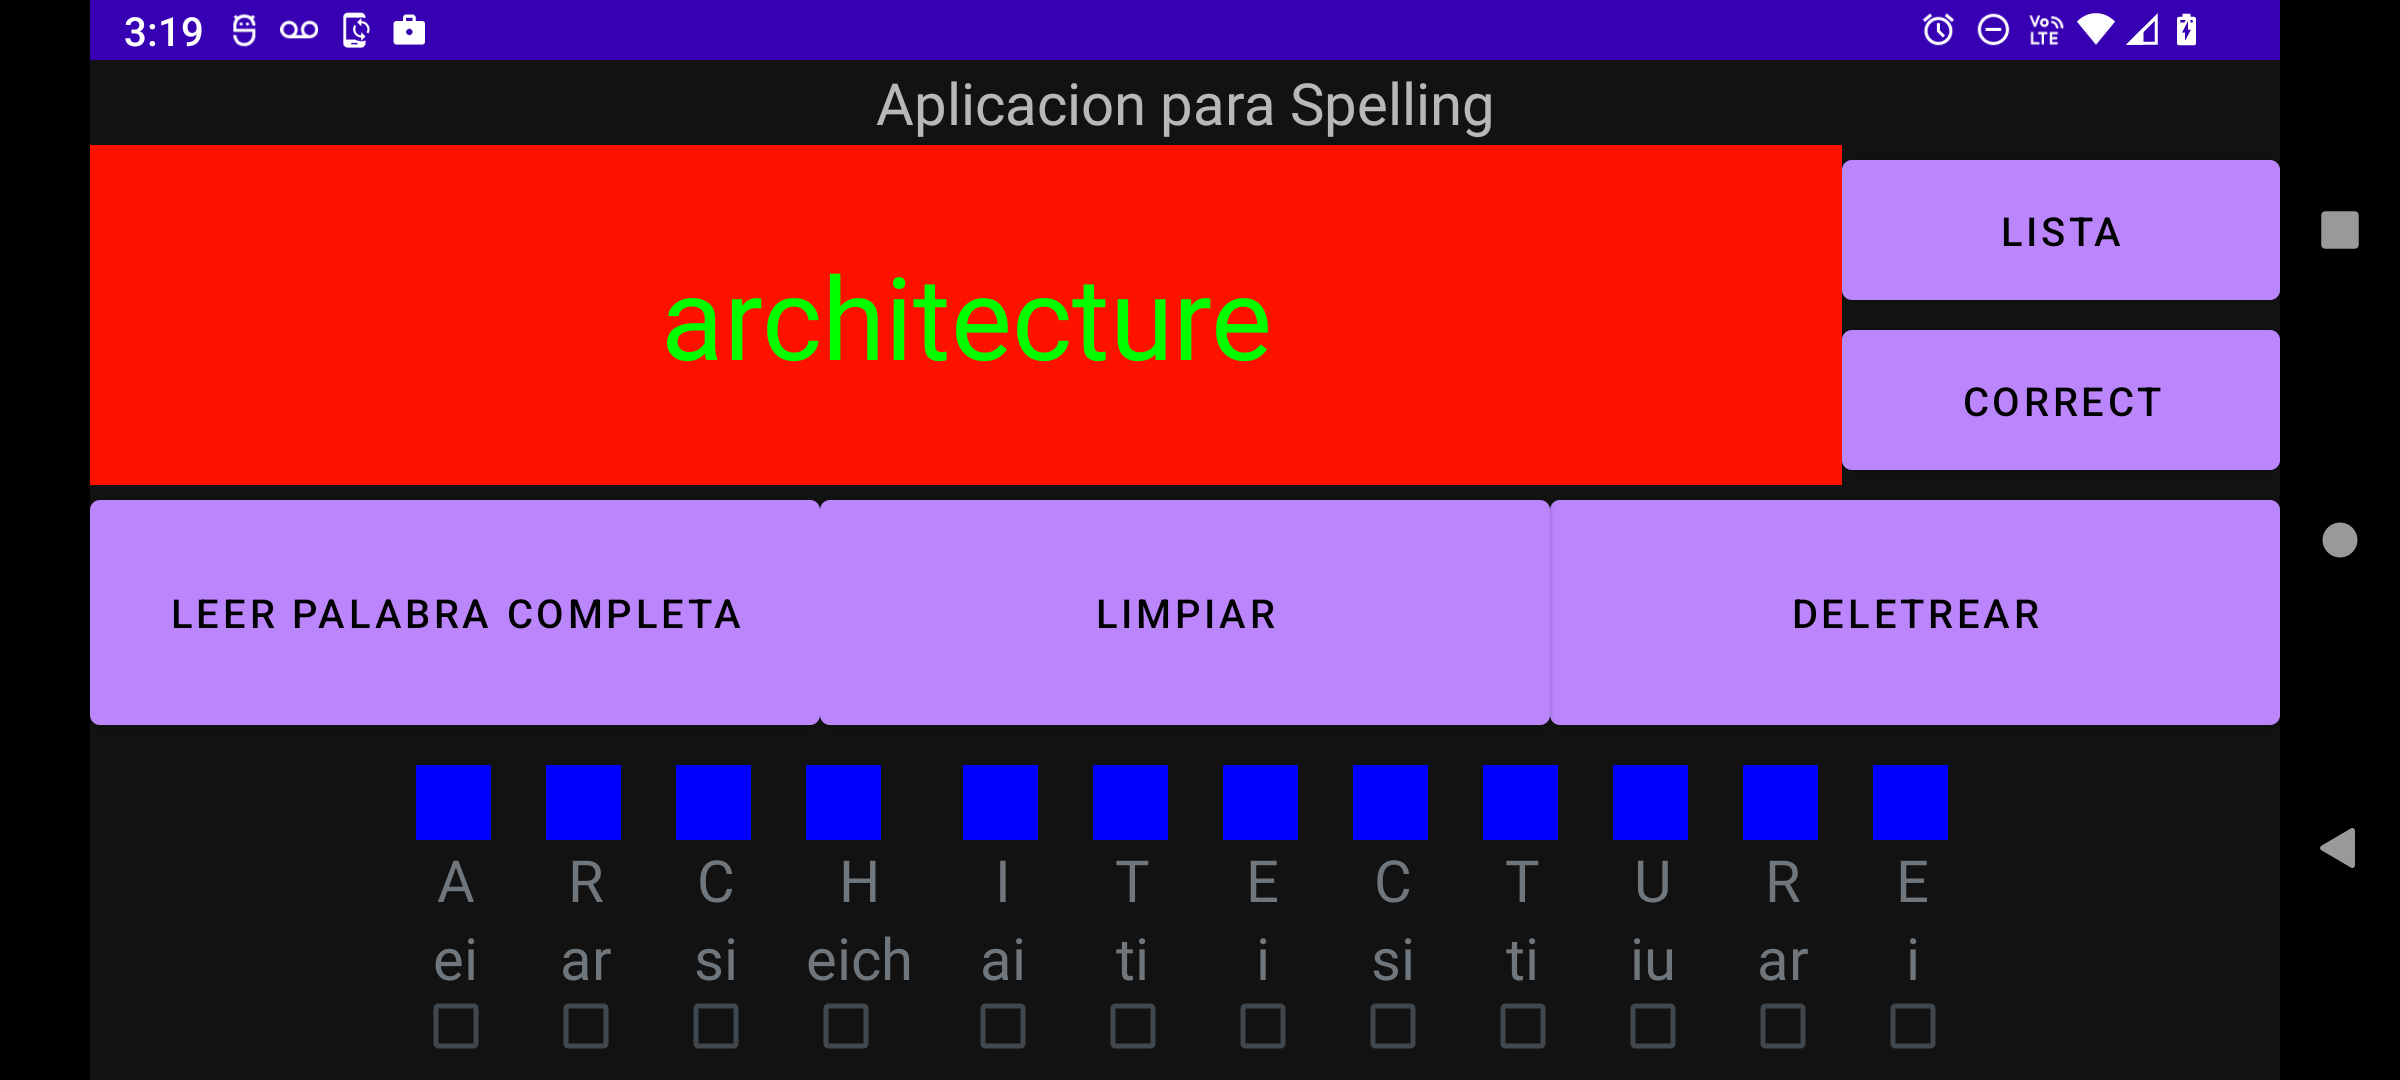
\includegraphics[width=0.46\linewidth]{2022_Spelling/figs/Spelling0.png} &
		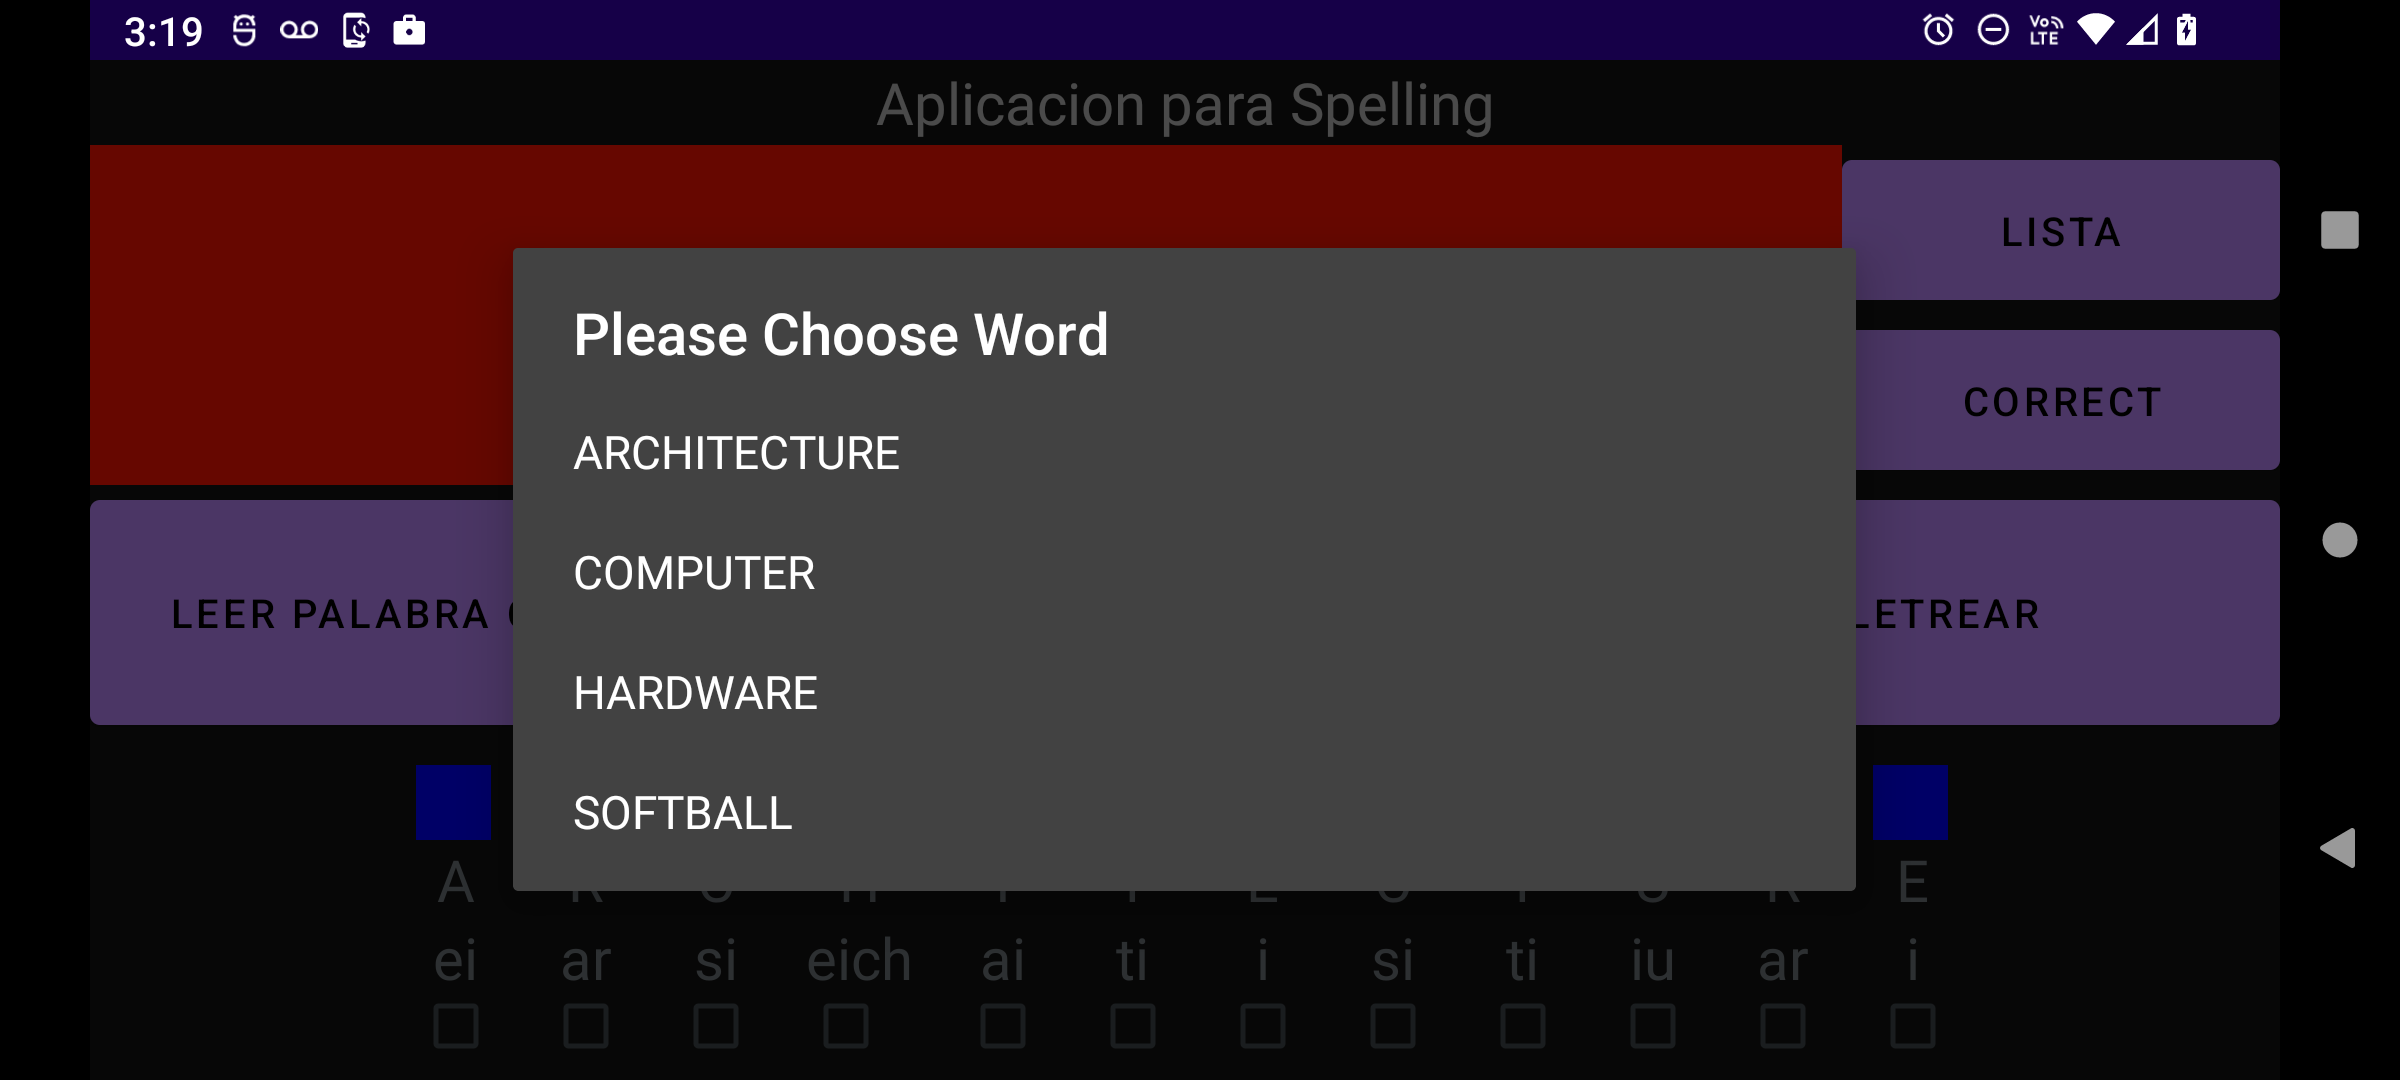
\includegraphics[width=0.46\linewidth]{2022_Spelling/figs/Spelling1.png} \\ 		 		
		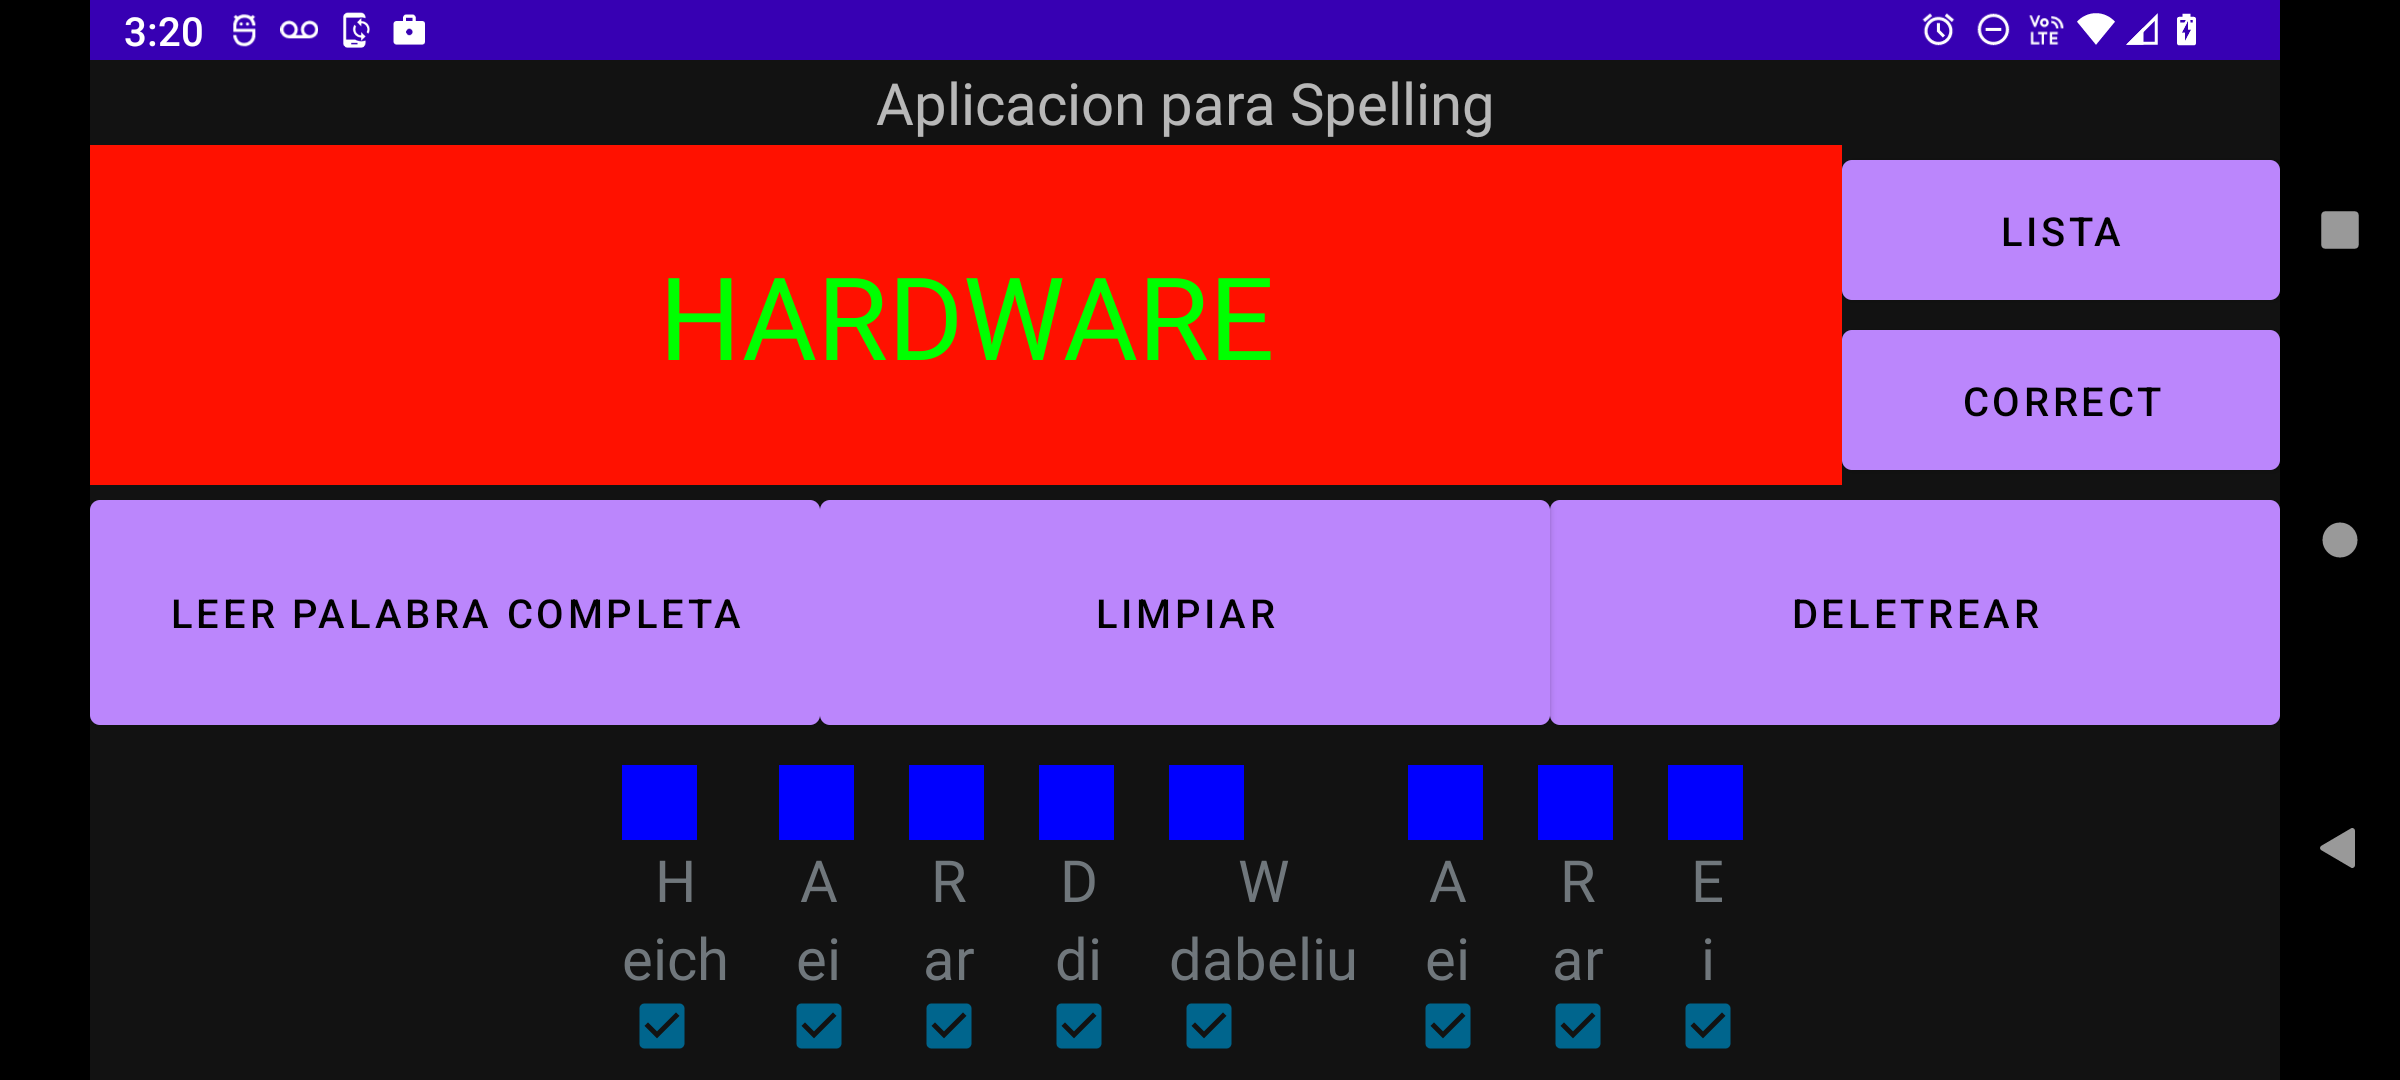
\includegraphics[width=0.46\linewidth]{2022_Spelling/figs/Spelling2.png} & 		
		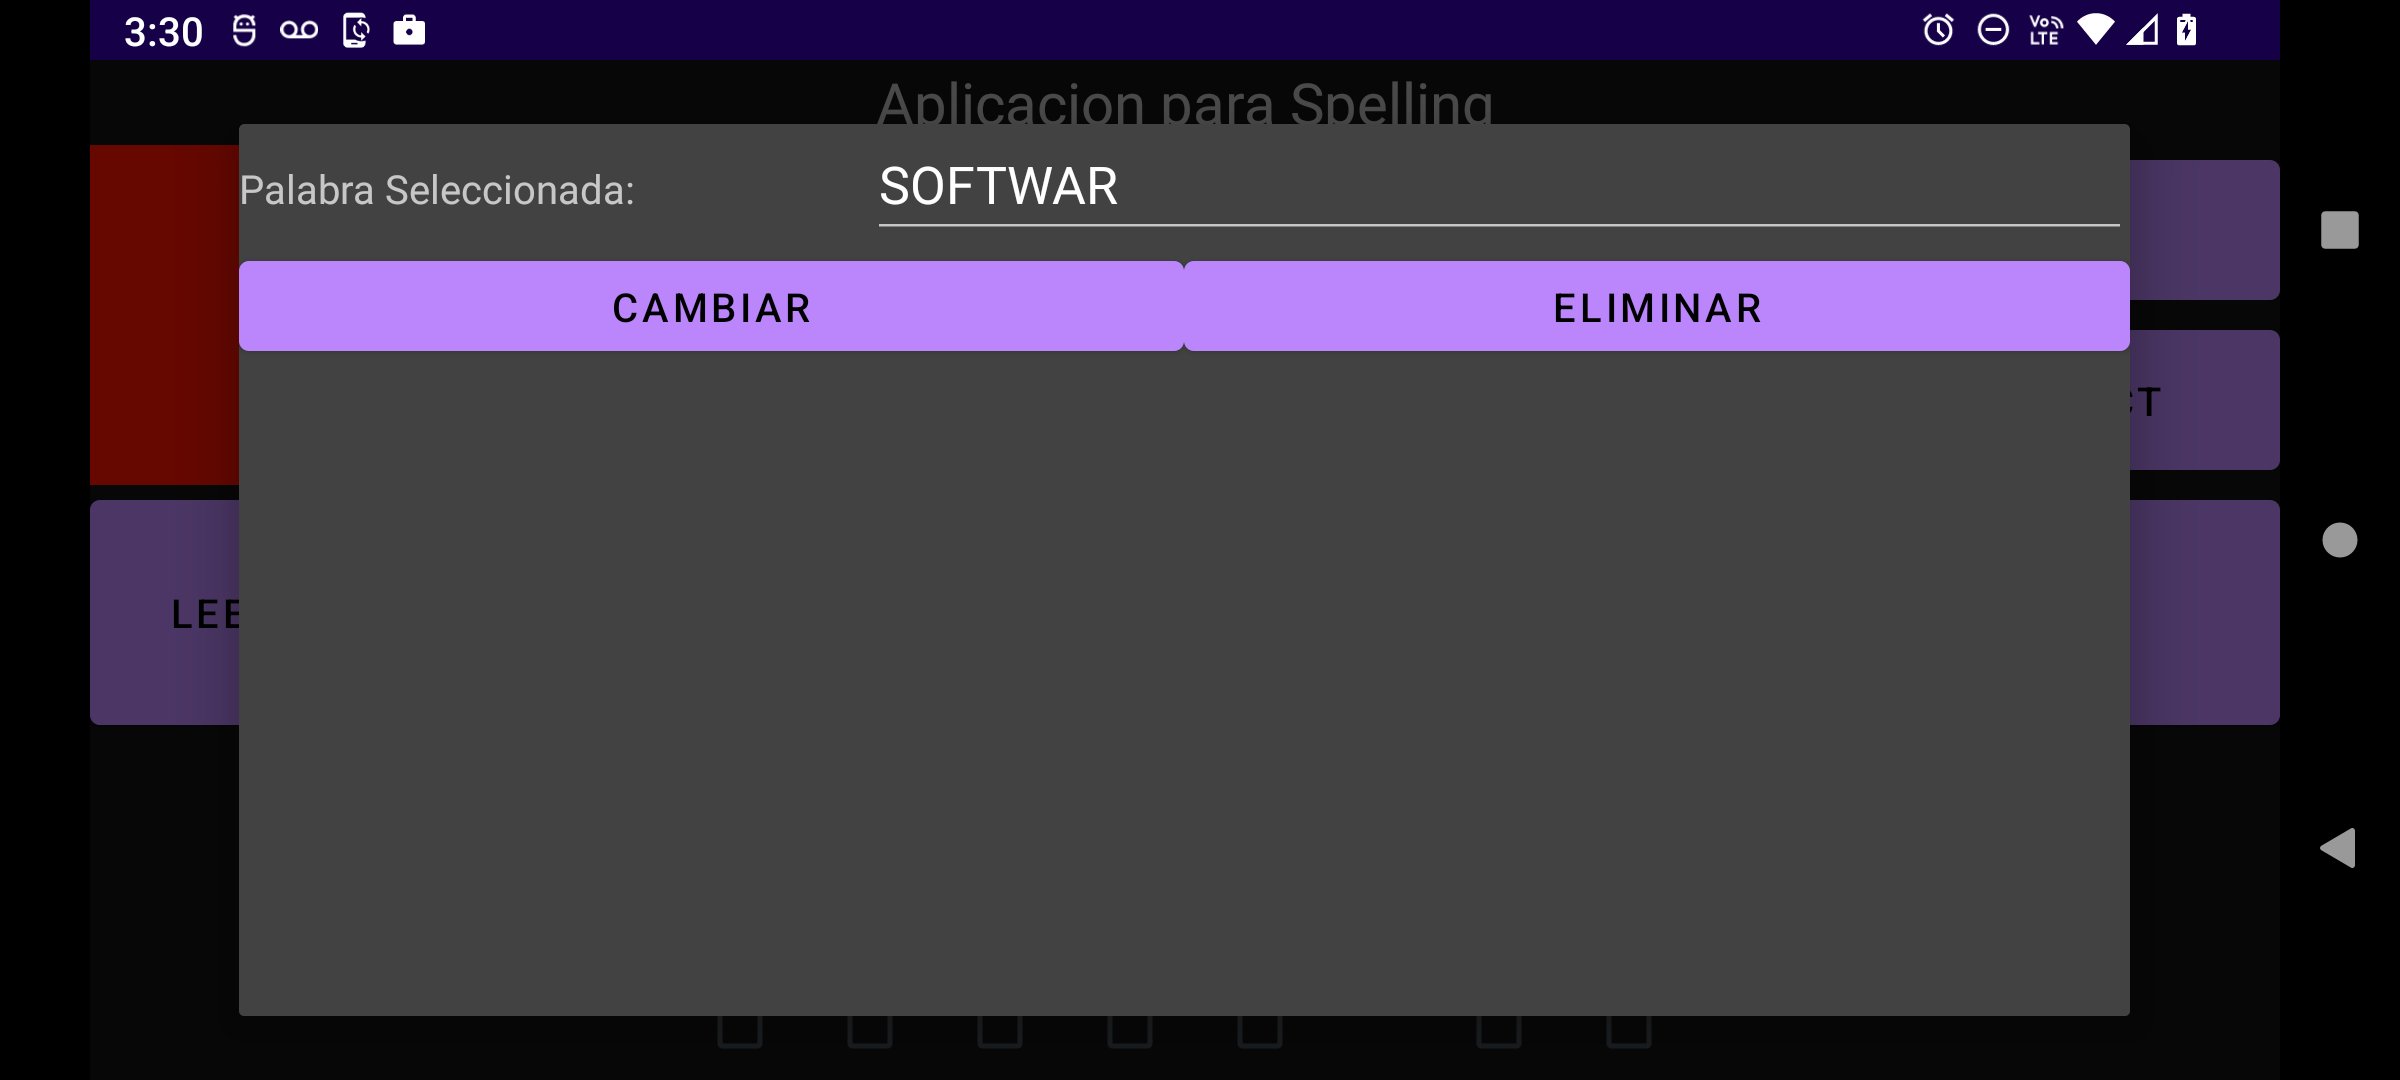
\includegraphics[width=0.46\linewidth]{2022_Spelling/figs/Spelling3.png} \\
	\end{tabular}
\end{center}
\end{frame}


%\renewcommand{\EntradaBibtex}{Escanner3D_Aleman2022}


\begin{frame}{\citetitle{\EntradaBibtex} \footnotemark[1] (1)}
\begin{columns}
\begin{column}{0.6\textwidth}
	\begin{itemize}
		\item Muchas de las tareas que tradicionalmente se hacían en una PC ahora han migrado hacia el teléfono inteligente
        \item La digitalización de objetos 3D ha tenido un auge en tiempos recientes
		\item El escaner se obtiene datos de un sensor ultrasónico montado en un motor (escaneo vertical)
		\item Una plataforma giratoria rota el objeto para obtener los datos desde todos los ángulos
	\end{itemize}
\end{column}
\begin{column}{0.4\textwidth}  
\begin{center}
     \begin{tabular}{c}
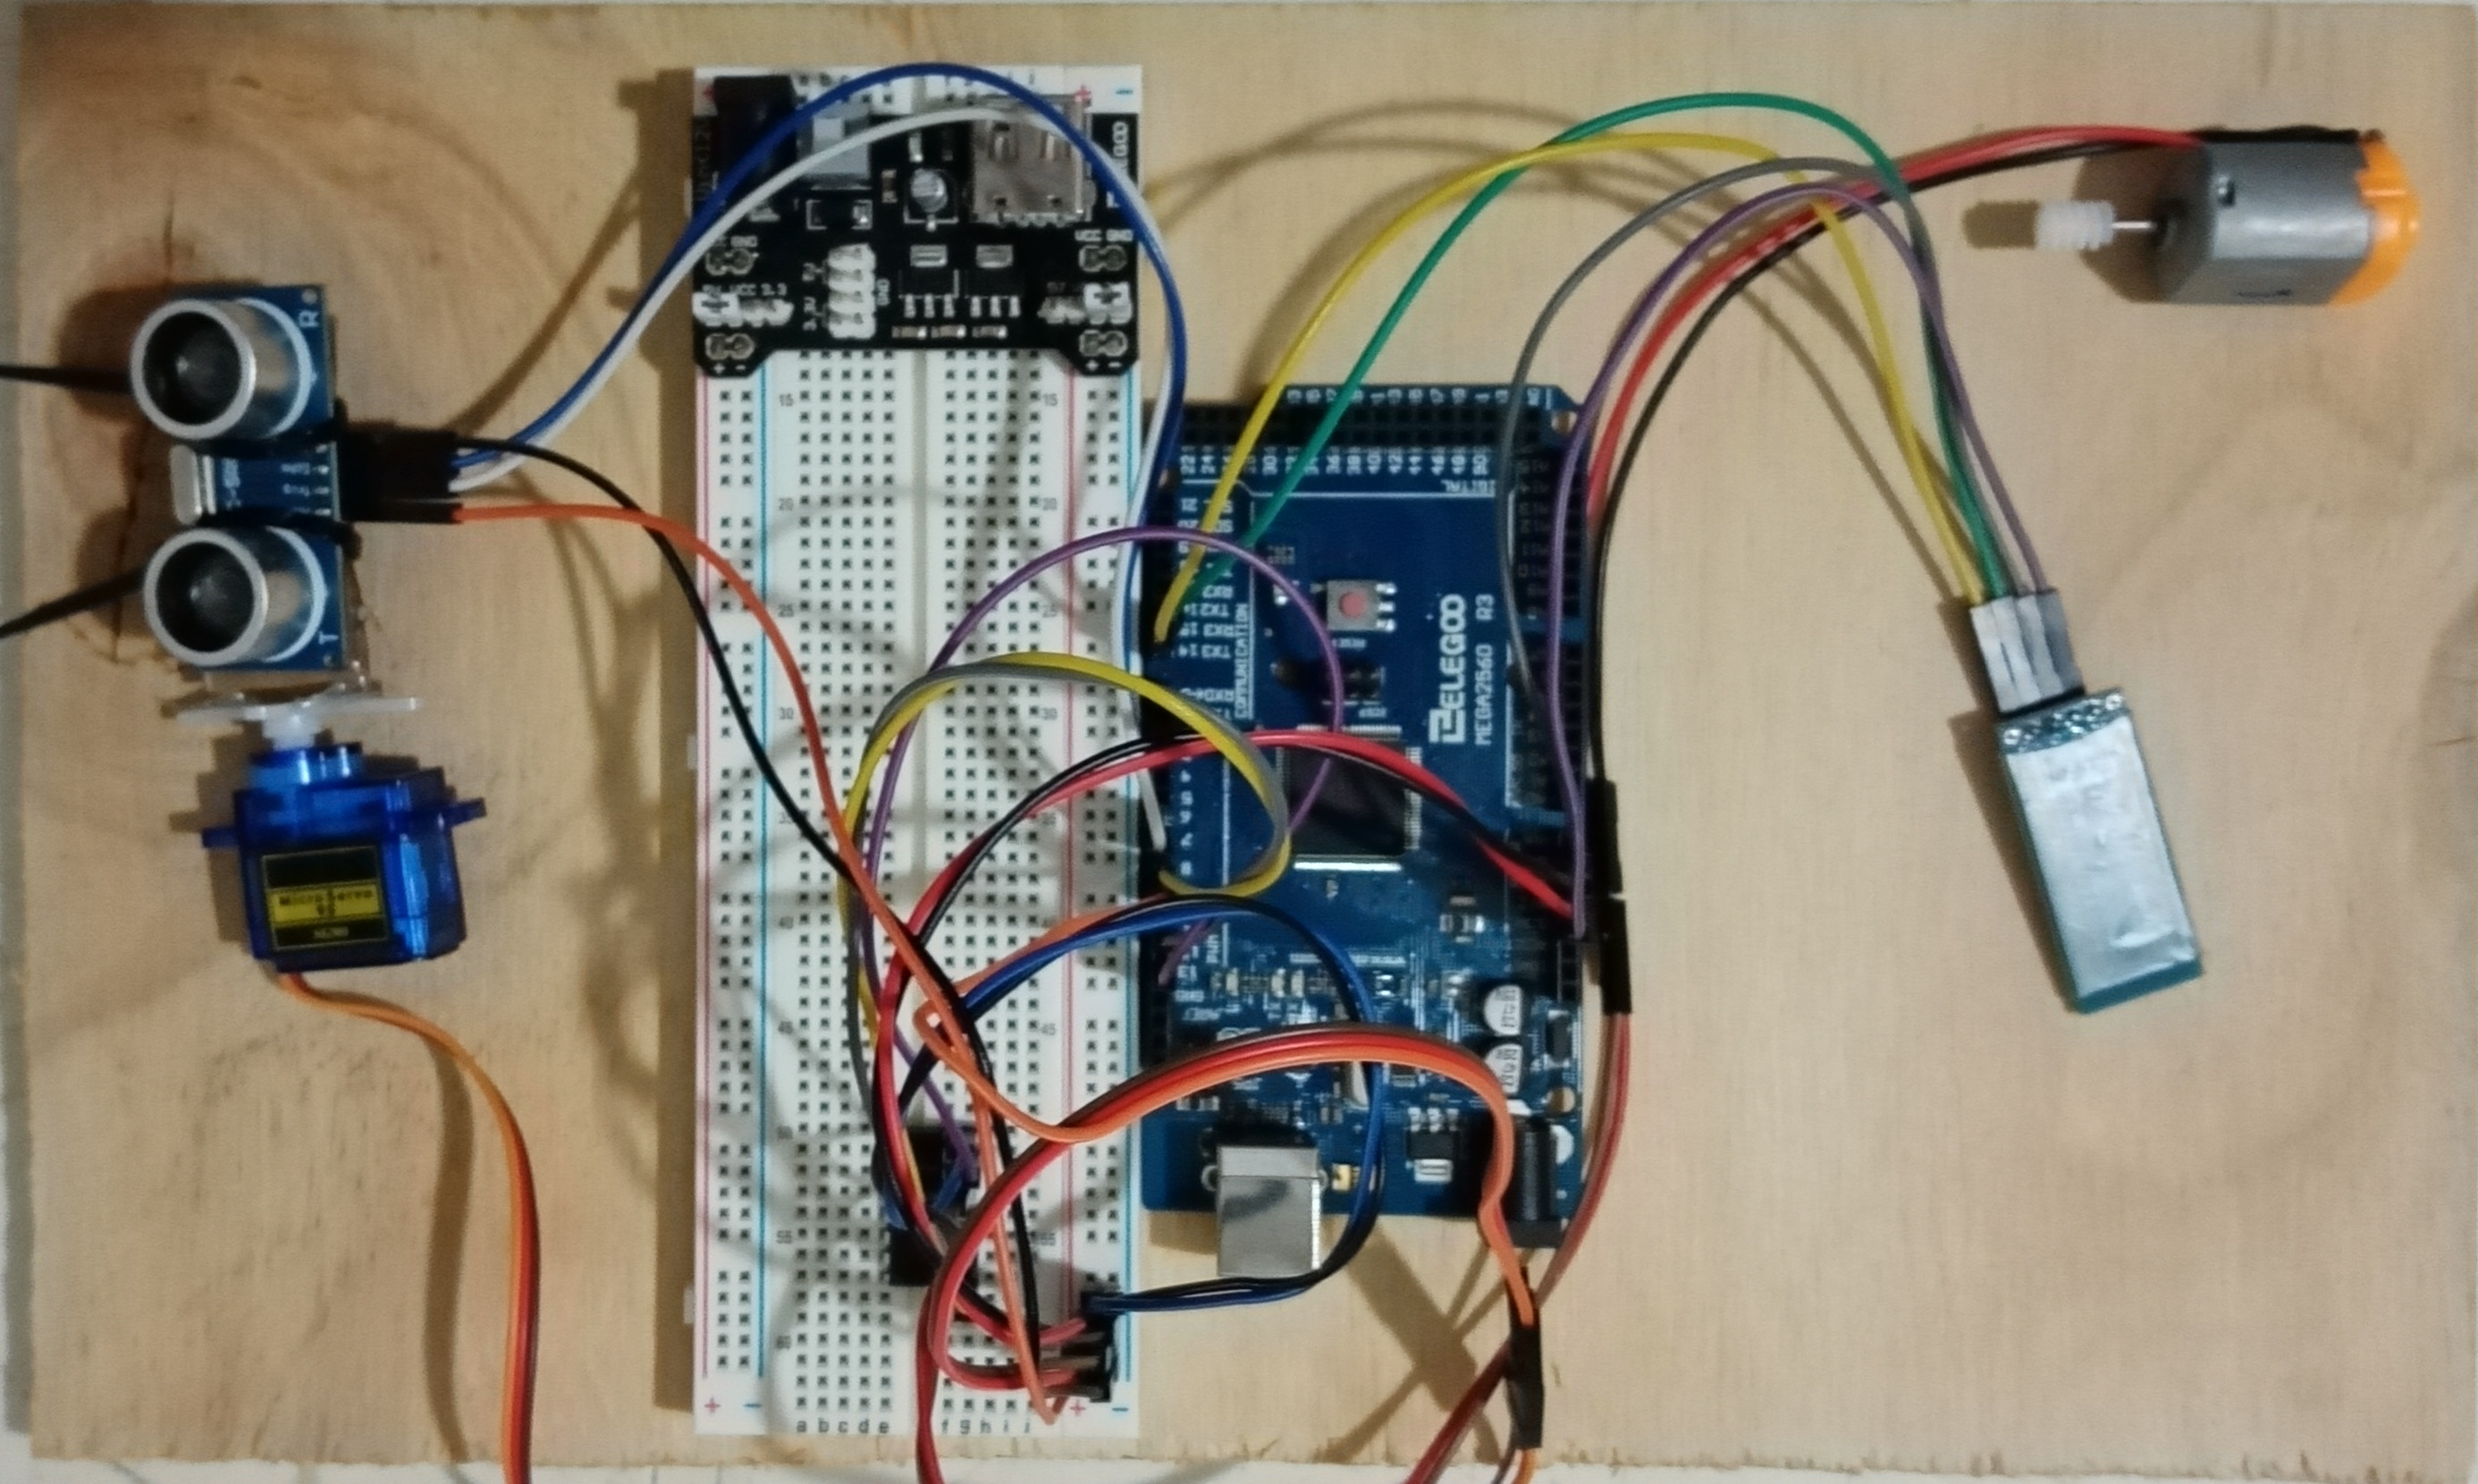
\includegraphics[width=0.68\textwidth]{2022_Scanner3D/figs/Esc1}\\
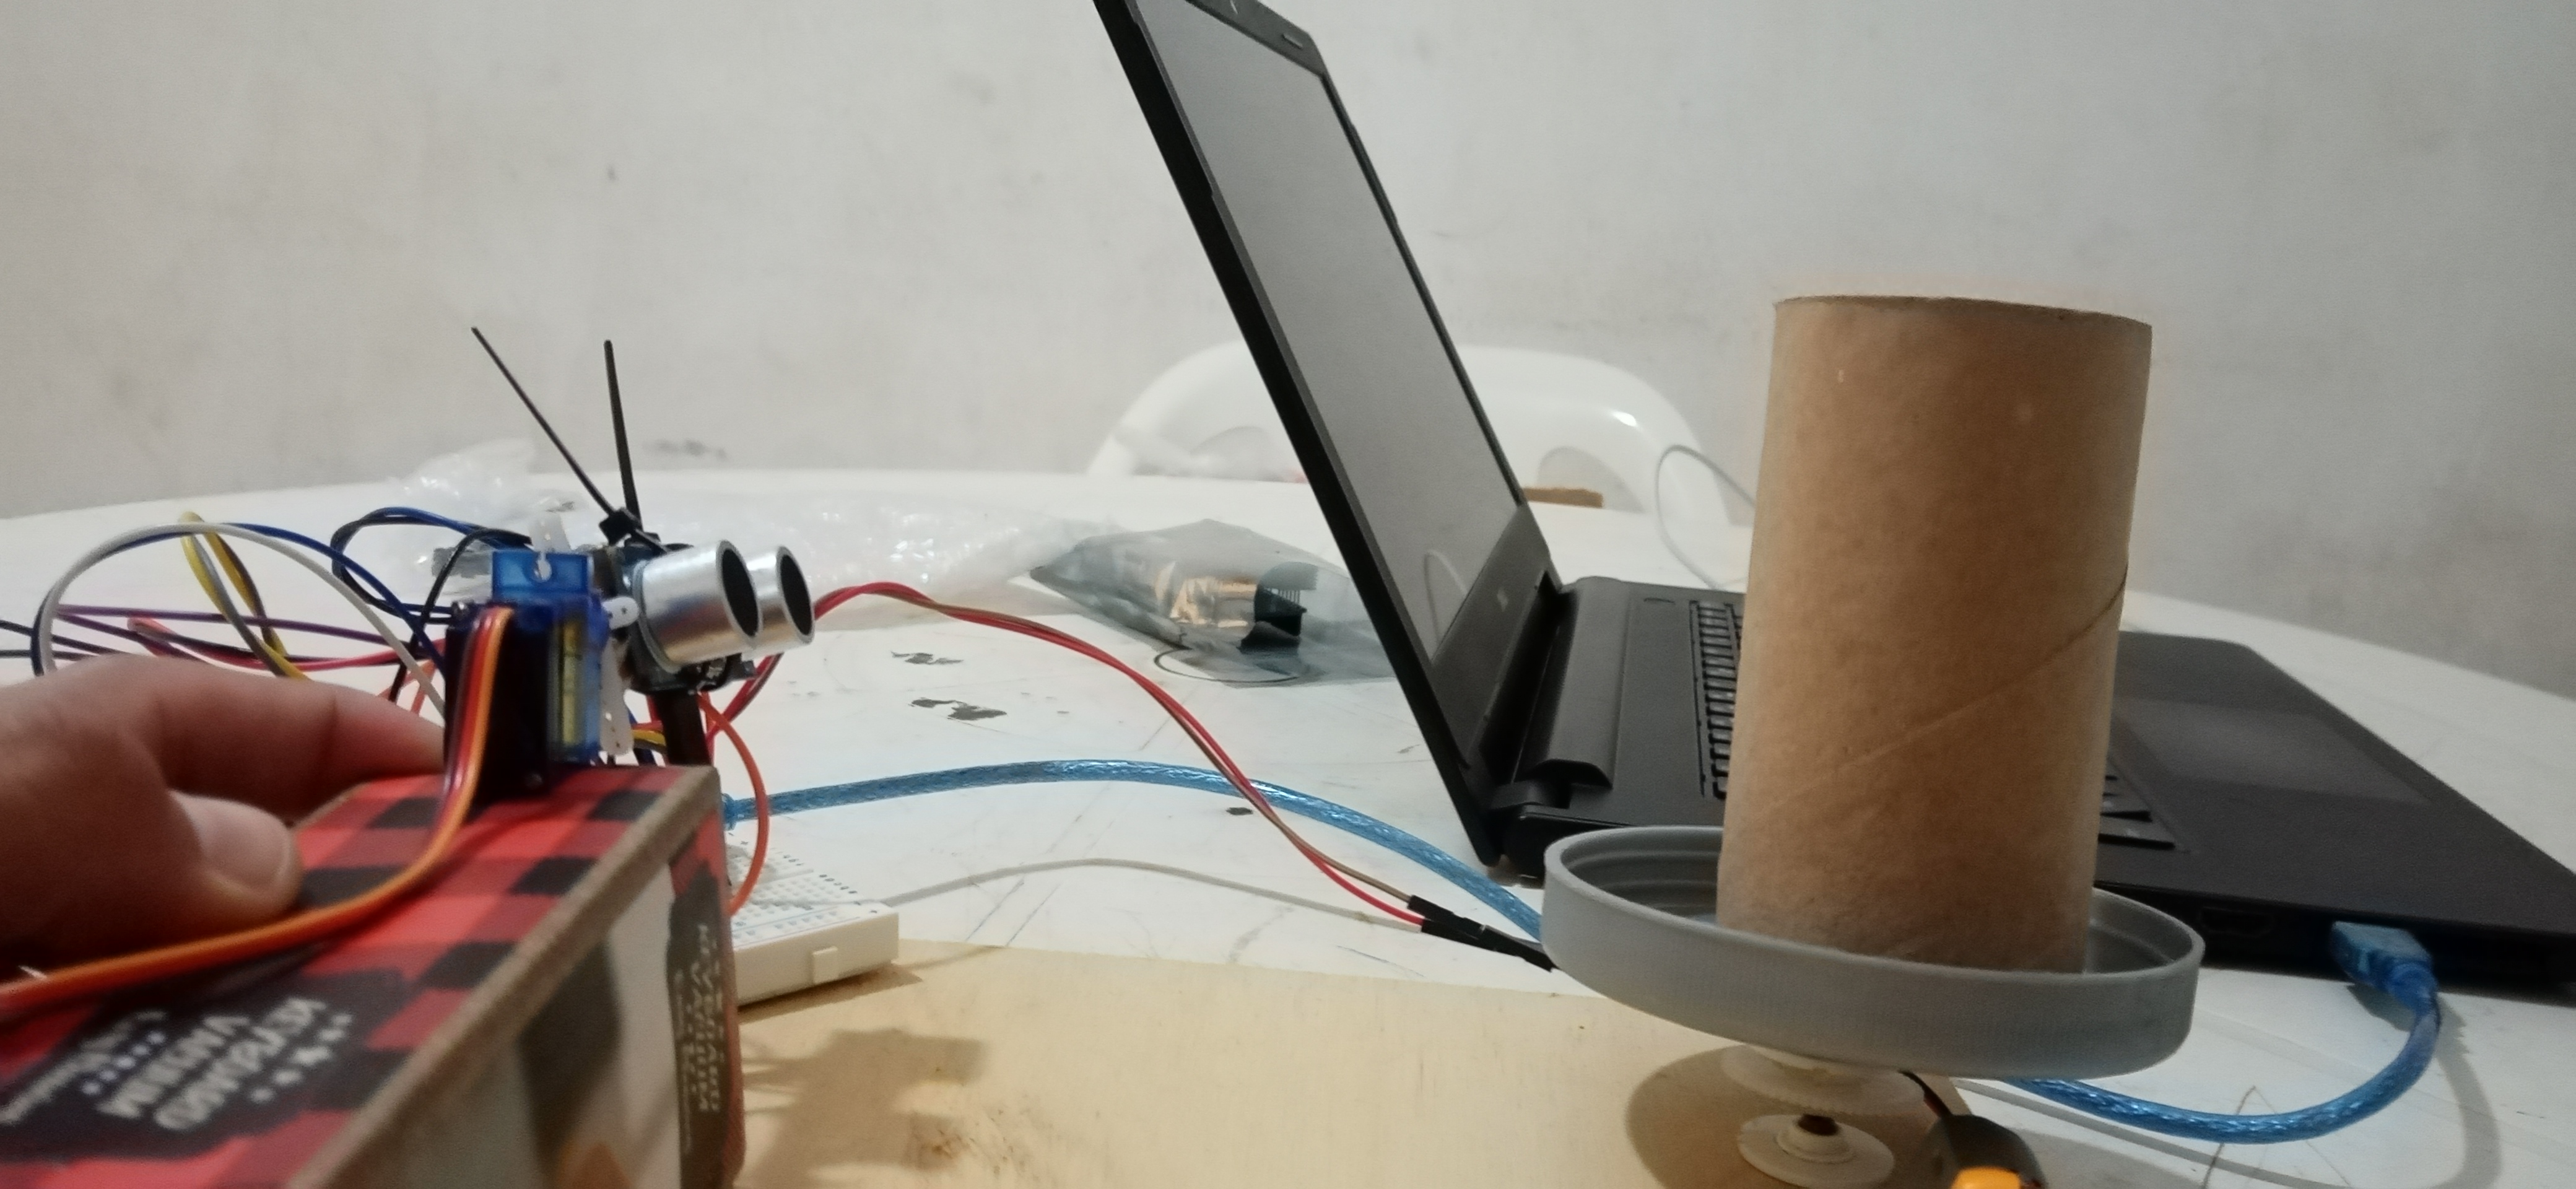
\includegraphics[width=0.68\textwidth]{2022_Scanner3D/figs/Esc2}\\         
      \end{tabular}
\end{center}
\end{column} 
\end{columns} 
\footnotetext[1]{\fullcite{\EntradaBibtex}}
\end{frame}


\begin{frame}{\citetitle{\EntradaBibtex} (2)}
	\begin{itemize}
        \item La aplicación visualiza el modelo adquirido y lo almacena en un formato estándar
        \item Se propone una App para un escaner 3D ``casero'' mediante comunicación Bluetooth
	\end{itemize}
\begin{center}
 \begin{tabular}{cccc}
    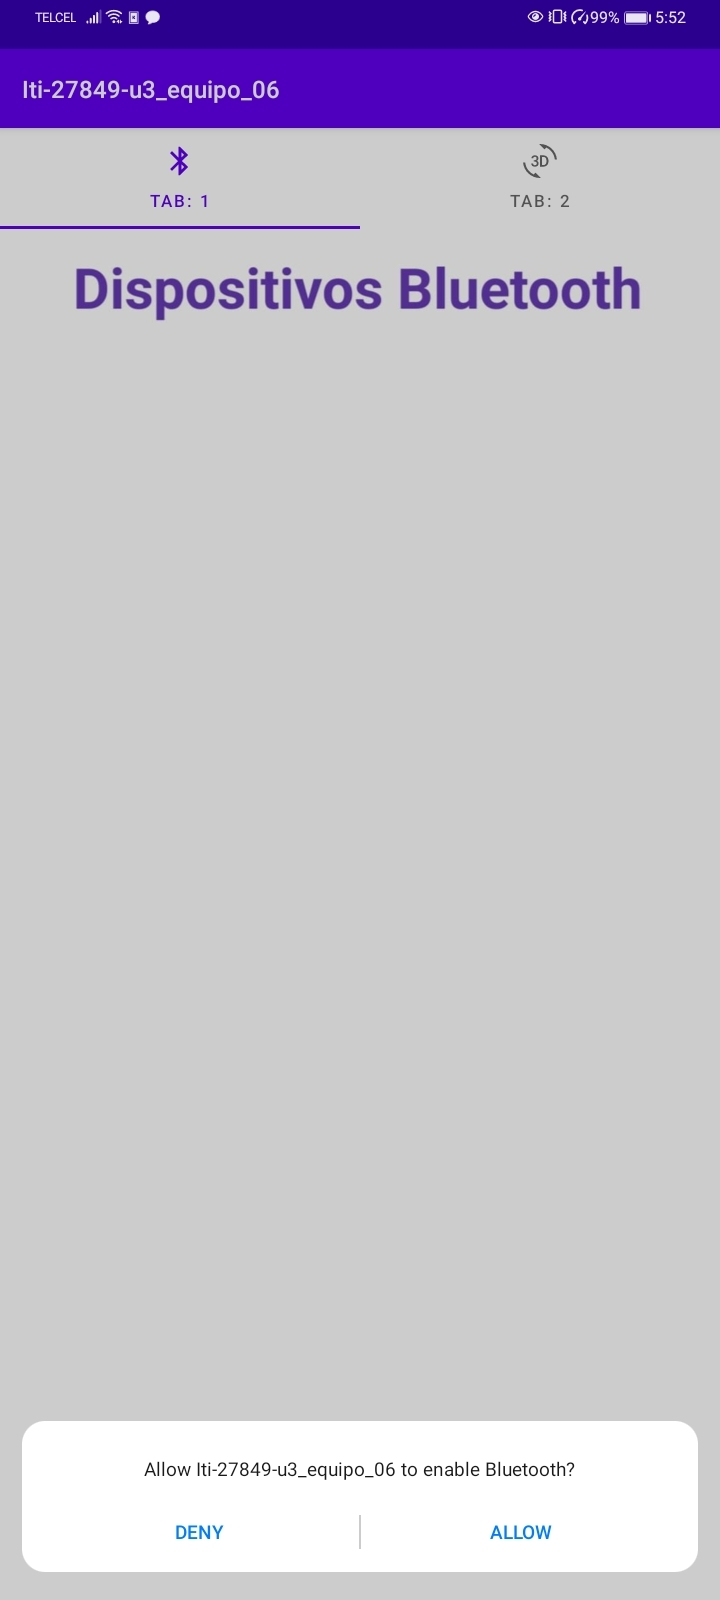
\includegraphics[width=0.14\textwidth]{2022_Scanner3D/figs/Ap1}
    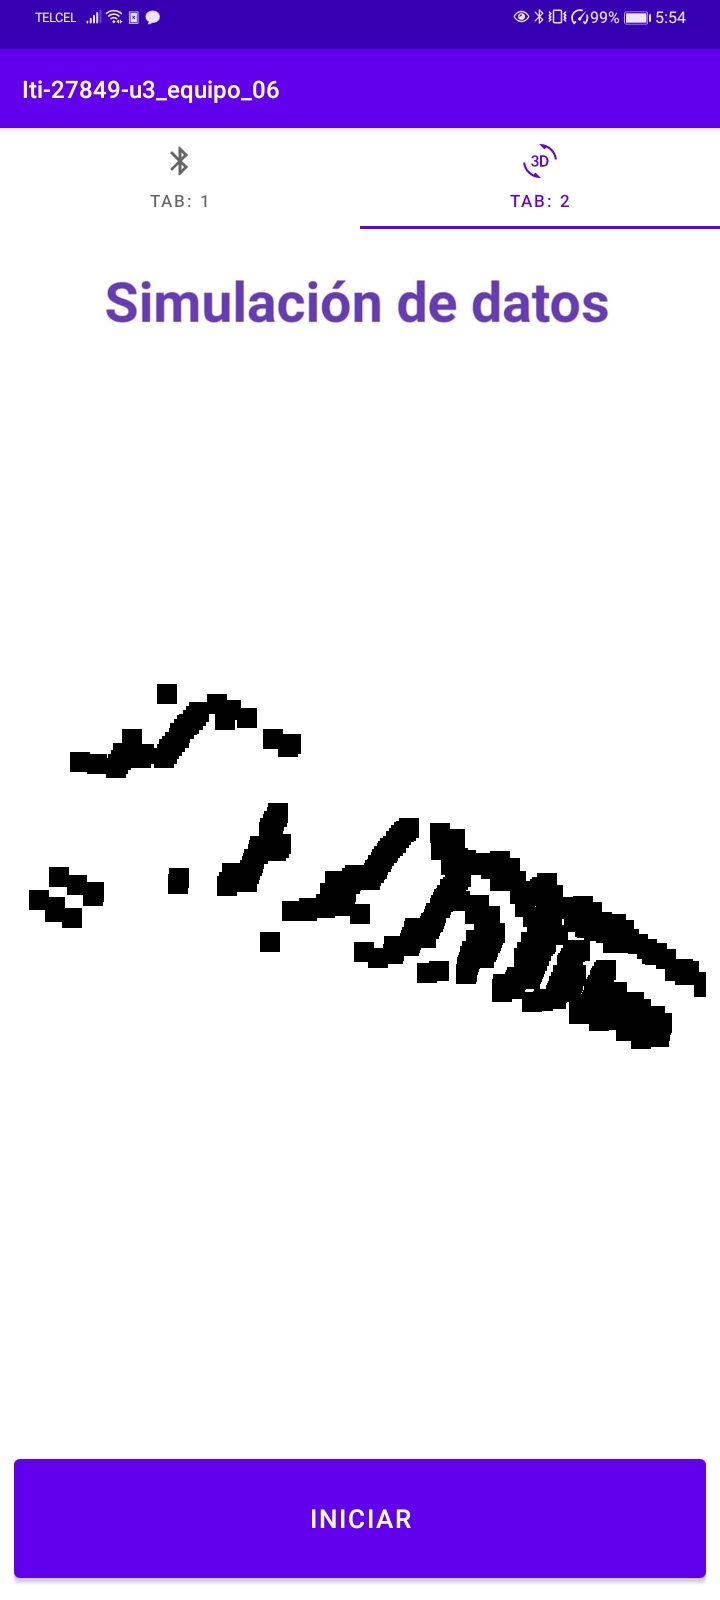
\includegraphics[width=0.14\textwidth]{2022_Scanner3D/figs/Ap2}
    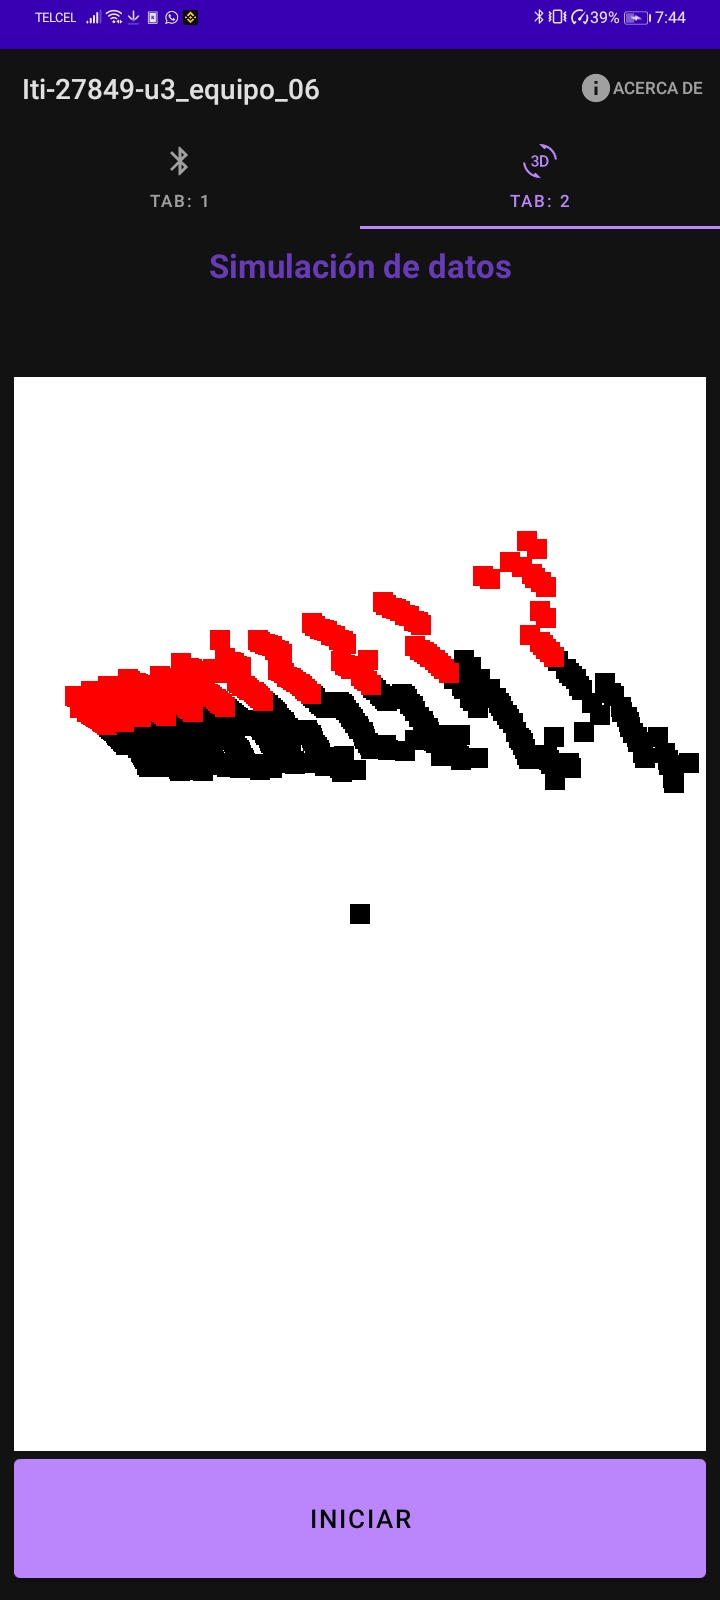
\includegraphics[width=0.14\textwidth]{2022_Scanner3D/figs/Ap3}
    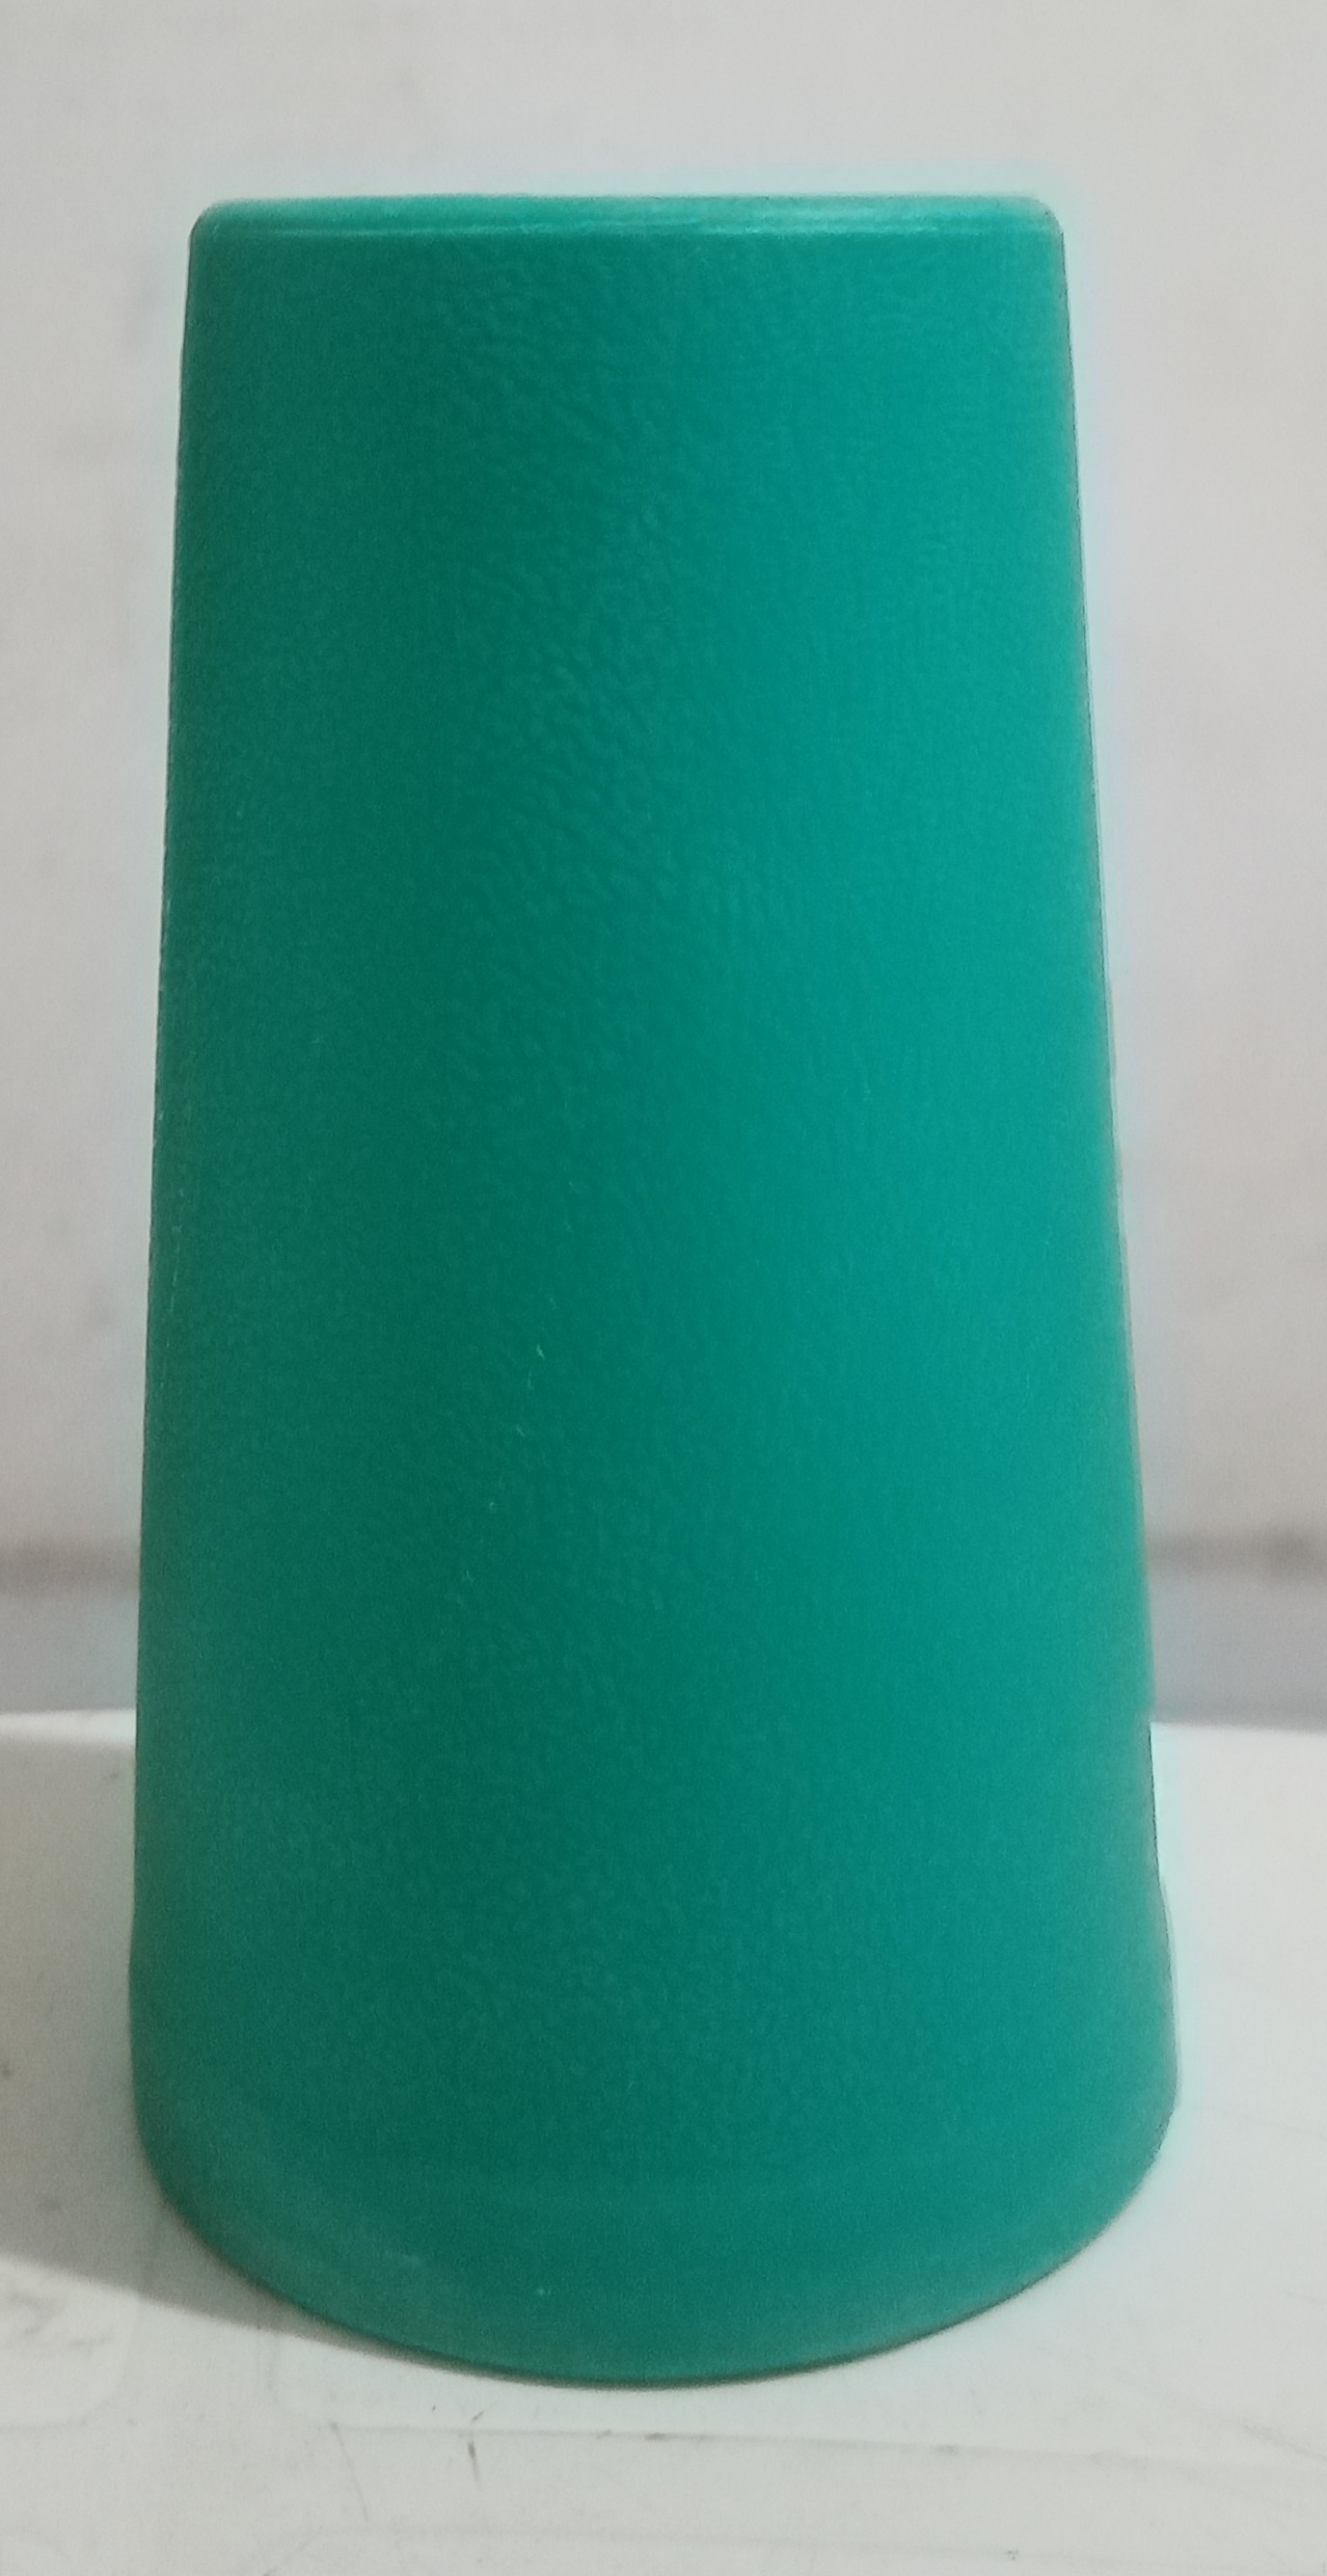
\includegraphics[width=0.16\textwidth]{2022_Scanner3D/figs/Ap4}
  \end{tabular}
\end{center}

\end{frame}







%
\renewcommand{\EntradaBibtex}{ProyectoRefrigeradoresFrios_2022}

\begin{frame}{\citetitle{\EntradaBibtex} \footnotemark[1] (1)}
\begin{columns}
\begin{column}{0.65\textwidth}
	\begin{itemize}  %del cuerpo académico Acuicultura Sustentable (UTMTB-CA-1)
        \item La Secretaría de Salud del de Tamaulipas almacena en refrigeradores y cámaras frías biológico (vacunas)
        \item Personal de las unidades de salud realiza registros y emite alarmas en situaciones anómalas
		\item Se propone un sistema capaz de vigilar remotamente (24/7) las variables de temperatura, humedad y conexión a la red eléctrica
	\end{itemize}
\end{column}
\begin{column}{0.35\textwidth}  
\begin{center}
     \begin{tabular}{cc}
         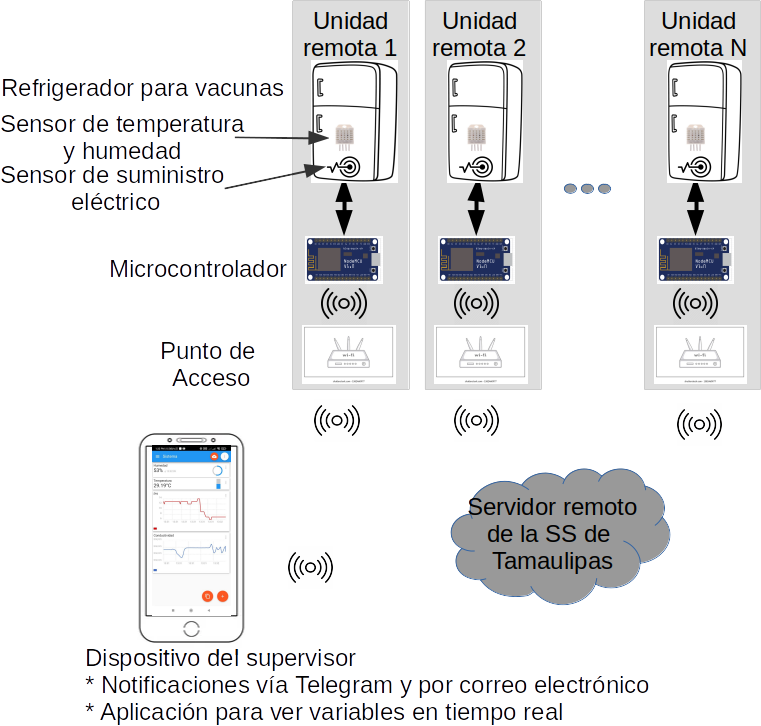
\includegraphics[width=0.98\textwidth]{2022_RefrigeradoresFrios/figs/SistemaRefrigeradoresFrios}\\         
      \end{tabular}
\end{center}
\end{column} 
\end{columns} 
\footnotetext[1]{\fullcite{\EntradaBibtex}}
\end{frame}


\begin{frame}{\citetitle{\EntradaBibtex} (2)}
\begin{columns}
\begin{column}{0.8\textwidth}
Resultados:
\begin{itemize}
    \item Se construyeron 325 dispositivos sensores, un sistema de información (para monitorear alarmas y valores de los sensores en rangos específicos de tiempo) y una aplicación movil
    \item Se han instalado dispositivos de monitoreo en 109 de 321 refrigeradores de la SST en 32 municipios de Tamaulipas
    \item Al cierre de esta presentación, se generaron más de 200 alarmas que han obligado a los responsables a verificar el estado de los refrigeradores
	\end{itemize}
\end{column}
\begin{column}{0.2\textwidth}  
\begin{center}
     \begin{tabular}{c}
         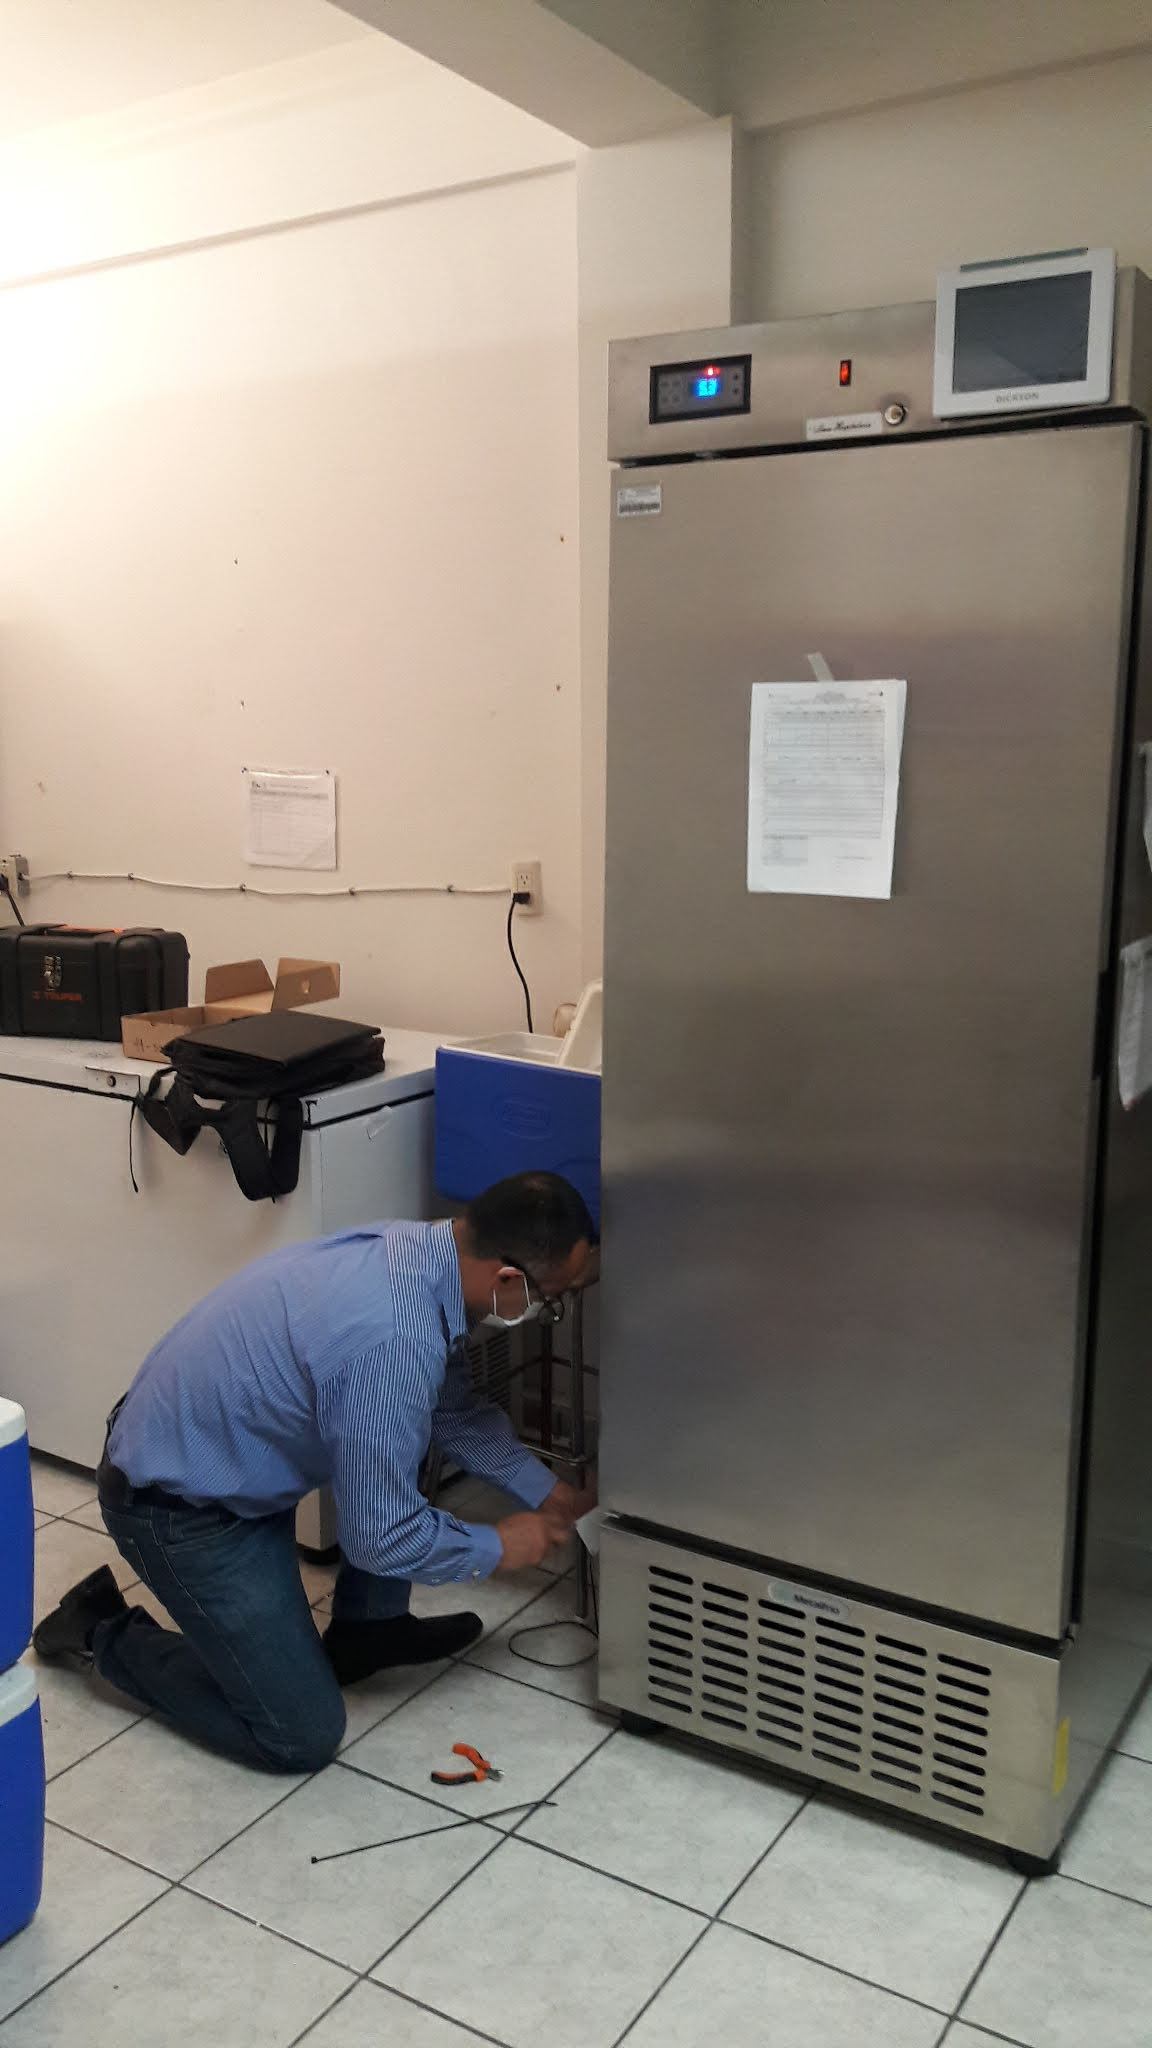
\includegraphics[width=0.98\textwidth]{2022_RefrigeradoresFrios/figs/RefrisSST}\\
          \end{tabular}
\end{center}
\end{column} 
\end{columns} 
\end{frame}





%
\renewcommand{\EntradaBibtex}{MarcoNuno_Revista_2022_10_00}

%\begin{frame}{\citetitle{MarcoNuno_Revista_2022_10_00}$^*$ (1)}
\begin{frame}{\citetitle{\EntradaBibtex} \footnotemark[1] (1)}
\begin{columns}
\begin{column}{0.99\textwidth}
	\begin{itemize}  %del cuerpo académico Acuicultura Sustentable (UTMTB-CA-1)
        \item Una aplicación eficaz para uso de transporte publico debe mostrar información acerca de las opciones de movilidad el usuario tiene en una localidad específica.
        \item En algunas localidades, esta información no esta disponible en las aplicaciones de mapas, lo que complica la movilidad del usuario.
		\item Se implementó una App específicamente para Ciudad Victoria, Tamps
	\end{itemize}
\end{column}
%\begin{column}{0.25\textwidth}  
%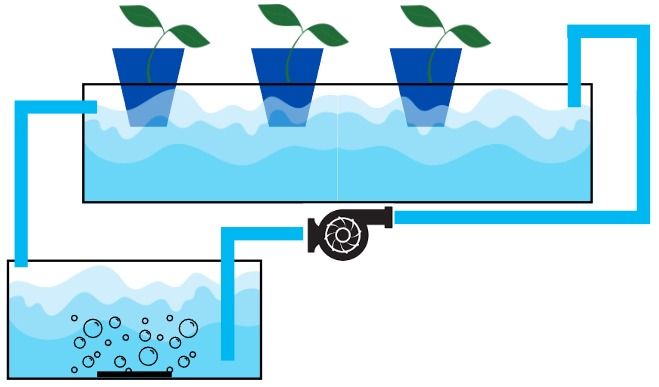
\includegraphics[width=0.98\textwidth]{2022_HidroponicosDavid/figs/dft}
%\end{column}
%\begin{column}{0.25\textwidth}
%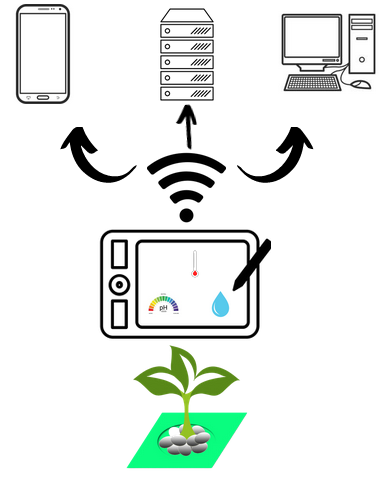
\includegraphics[width=0.98\textwidth]{2022_HidroponicosDavid/figs/iot}
%\end{column}
\end{columns} 
\footnotetext[1]{\fullcite{\EntradaBibtex}}
\end{frame}


\begin{frame}{\citetitle{\EntradaBibtex} (2)}
\begin{columns}
\begin{column}{0.25\textwidth}  
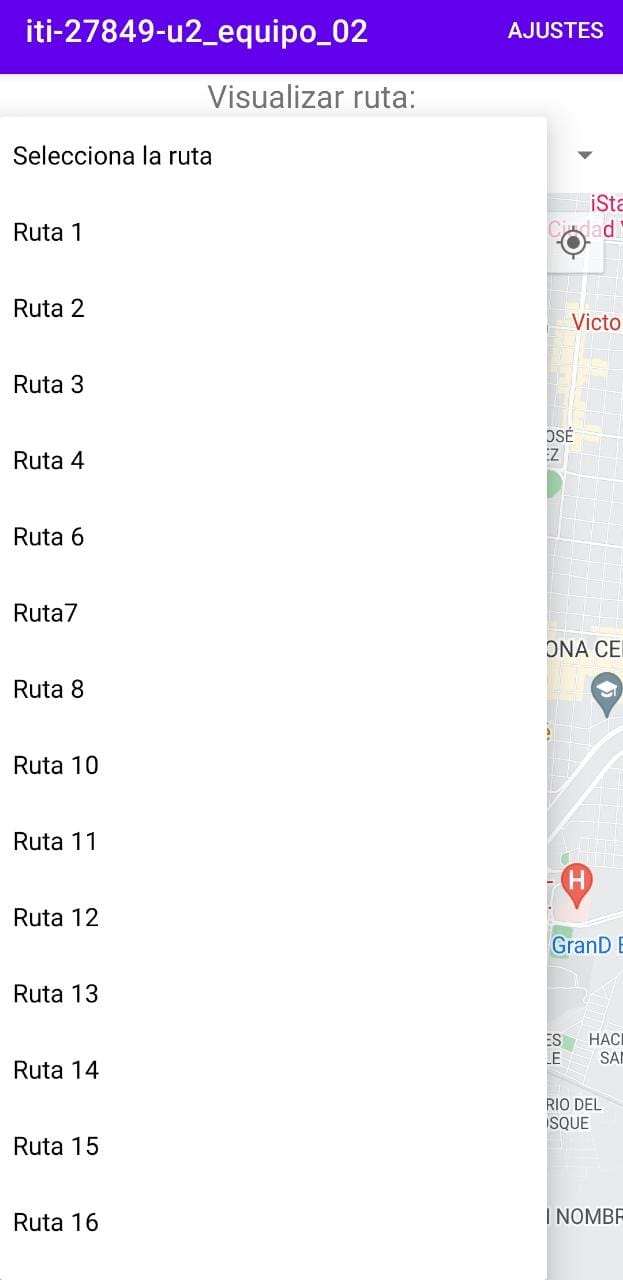
\includegraphics[width=0.82\textwidth]{2022_MapaVickyRanch/figs/F3}
\end{column}
\begin{column}{0.25\textwidth}  
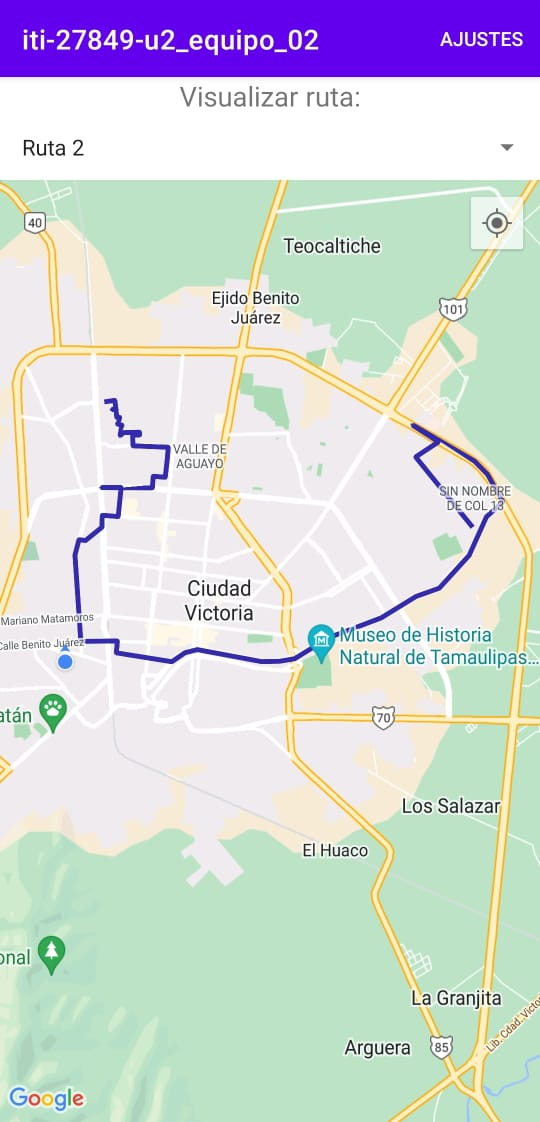
\includegraphics[width=0.82\textwidth]{2022_MapaVickyRanch/figs/F4}
\end{column}
\begin{column}{0.25\textwidth}  
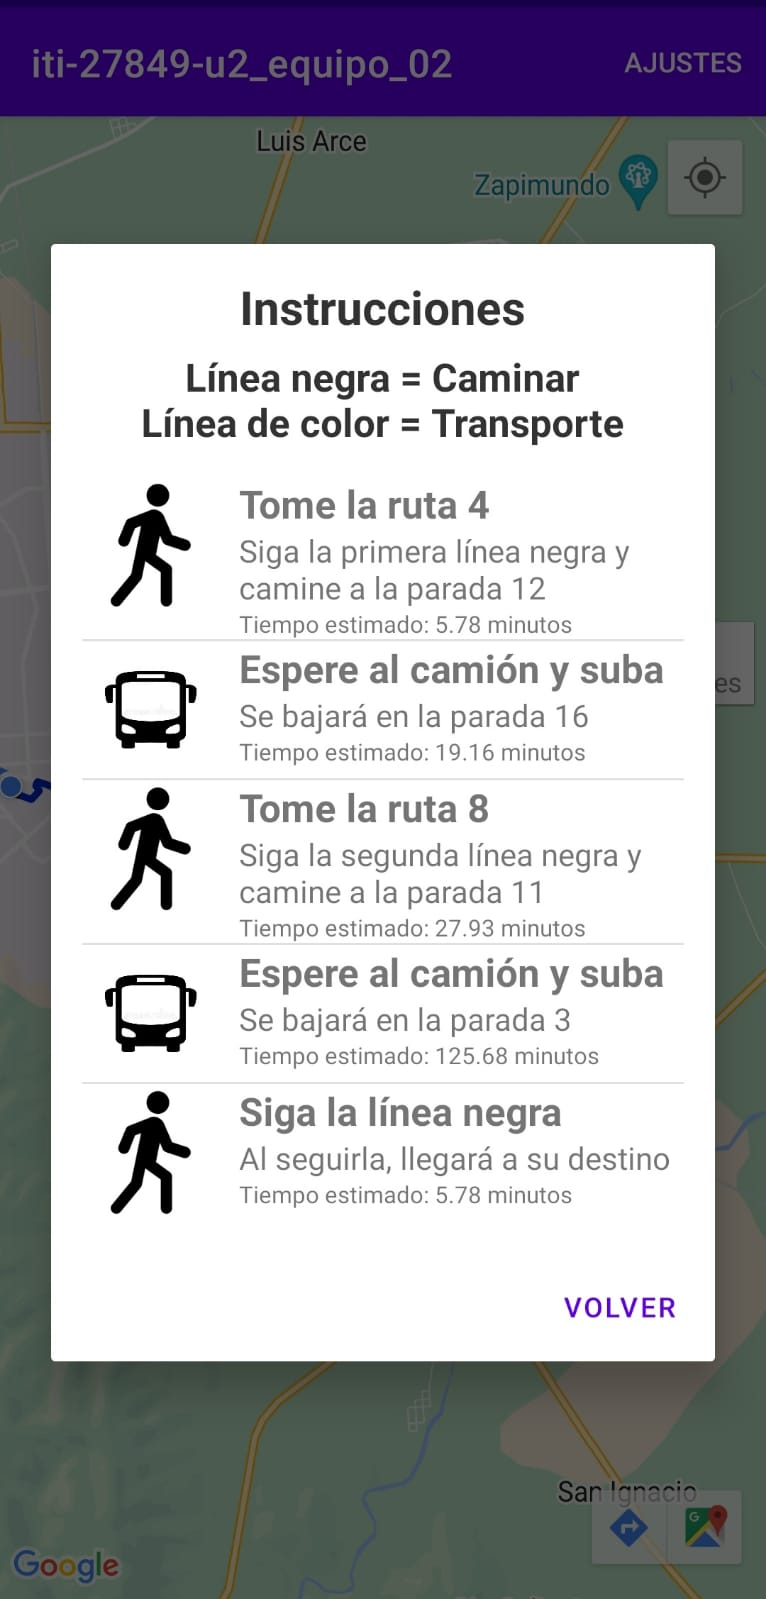
\includegraphics[width=0.82\textwidth]{2022_MapaVickyRanch/figs/F9}
\end{column}
\begin{column}{0.25\textwidth}  
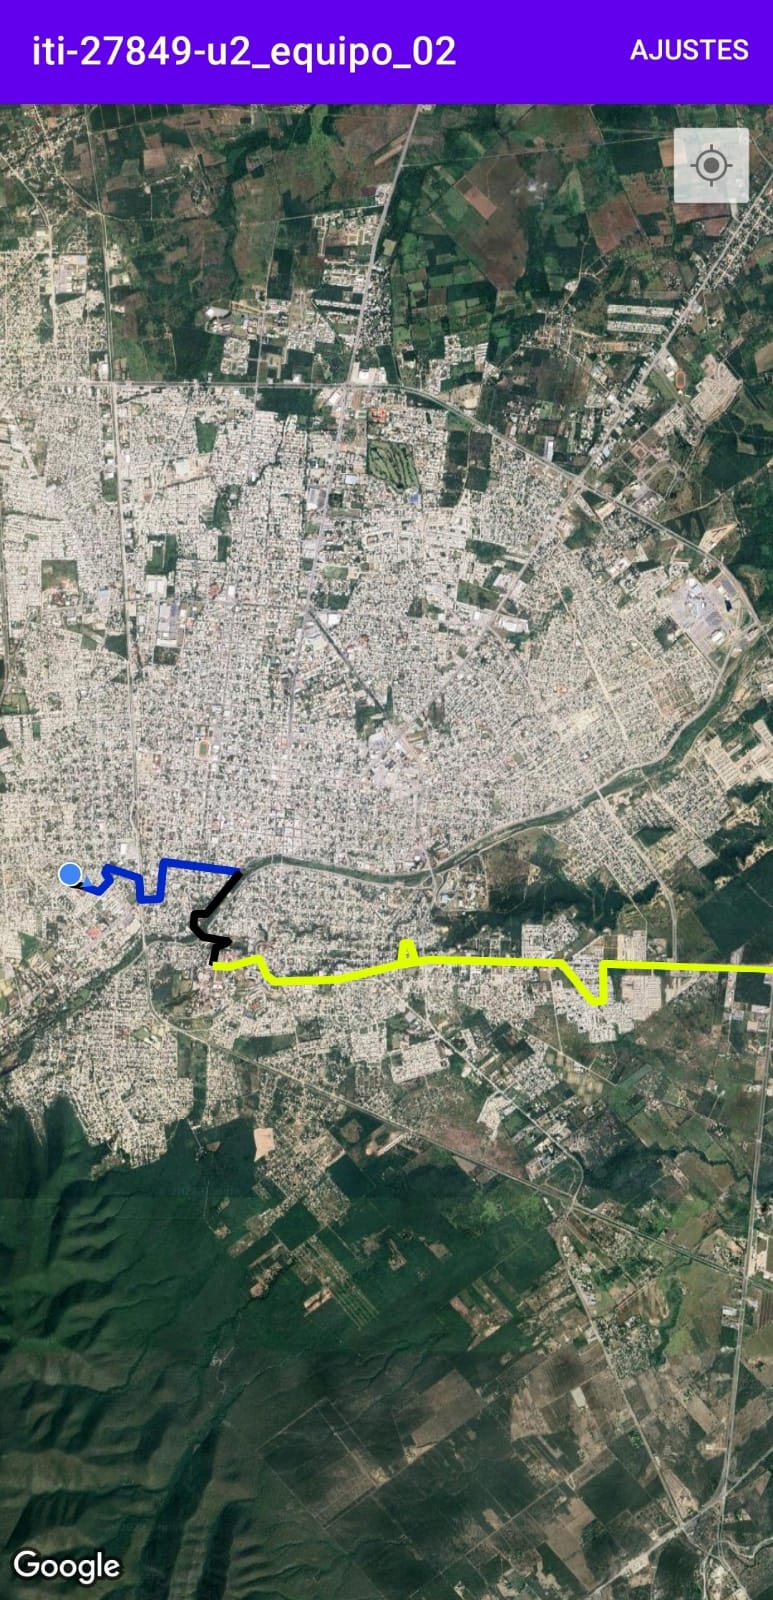
\includegraphics[width=0.82\textwidth]{2022_MapaVickyRanch/figs/F13}
\end{column}

\end{columns} 
\end{frame}


%
\renewcommand{\EntradaBibtex}{MarcoNuno_ReporteTecnico2022_B}

%\begin{frame}{\citetitle{MarcoNuno_ReporteTecnico2022_B}$^*$  (1)}
\begin{frame}{\citetitle{\EntradaBibtex} \footnotemark[1] (1)}
\begin{columns}
\begin{column}{0.70\textwidth}
	\begin{itemize}
		\item El chile piquín (\textit{Capsicum annuum L. var. aviculare}) es una producto endémico de la región noreste de la república mexicana
        \item Durante la cosecha, el fruto tiene que ser cortado junto con su pedúnculo
        \item Se desarrolló de una máquina que permita quitar el cabo en forma automática para agregar valor a su producción
	\end{itemize}
\end{column}
\begin{column}{0.30\textwidth}  
\begin{center}
     \begin{tabular}{cc}
         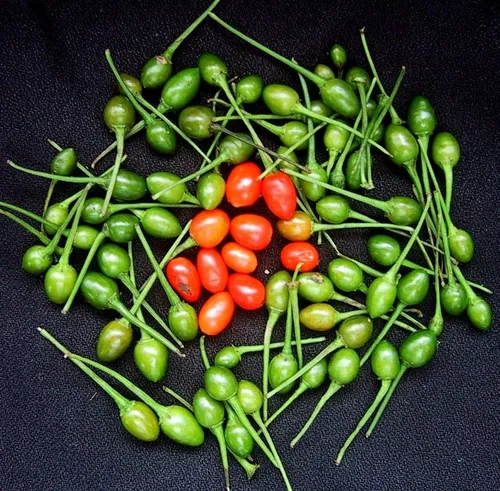
\includegraphics[width=0.68\textwidth]{2022_MaquinaChilePiquin/figs/TeSientas.png}\\         
      \end{tabular}
\end{center}
\end{column} 
\end{columns} 


%\footnotetext[1]{\fullcite{MarcoNuno_ReporteTecnico2022_C}}
%\setcounter{footnote}{0}
\footnotetext[1]{\fullcite{\EntradaBibtex}}
\end{frame}


\begin{frame}{\citetitle{\EntradaBibtex} (2)}
\begin{columns}
\begin{column}{0.50\textwidth}
Prototipo 1:
\begin{itemize}
        \item Un pistón neumático se accionaba para darle movimiento 
        \item El corte de los pedúnculo era efectuado por unas peinetas estratégicamente colocadas
        \item Llevaba a cabo el corte de manera eficaz, pero requeria del acomodo de los chiles
	\end{itemize}
\end{column}
\begin{column}{0.50\textwidth}  
\begin{center}
     \begin{tabular}{c}
         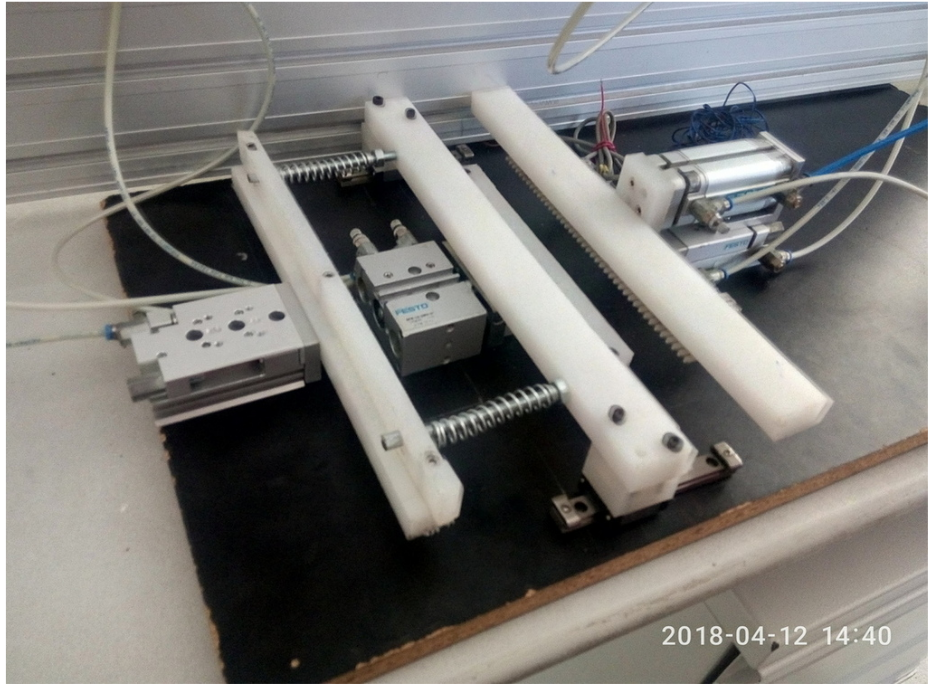
\includegraphics[width=0.98\textwidth]{2022_MaquinaChilePiquin/figs/Prototipo1.png}\\
          \end{tabular}
\end{center}
\end{column} 
\end{columns} 
\end{frame}



\begin{frame}{\citetitle{MarcoNuno_ReporteTecnico2022_B} (3)}
\begin{columns}
\begin{column}{0.55\textwidth}
Prototipo 2:
\begin{itemize}
        \item Se agregaron modificaciones para permitir el posicionamiento de
los chiles sin necesidad de intervención humana. 
        \item Usa sistemas neumáticos y eléctricos para accionar los diferentes mecanismos.
        \item Este prototipo realiza el desprendimiento de los pedúnculos, sin embargo todavía es necesaria la intervención humana para lograr una adecuada remoción de los mismos
	\end{itemize}
\end{column}
\begin{column}{0.45\textwidth}  
\begin{center}
     \begin{tabular}{c}
         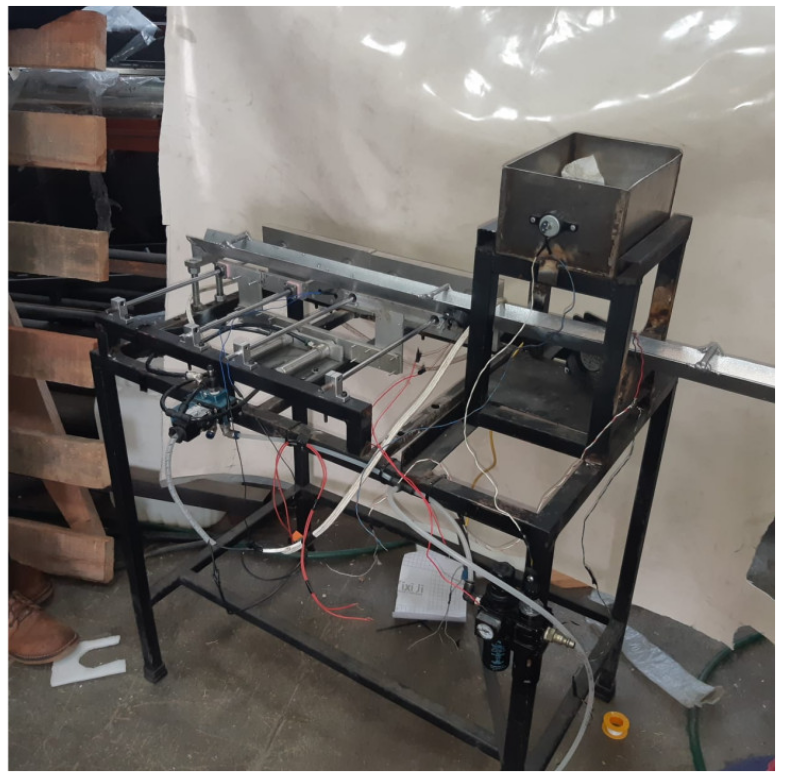
\includegraphics[width=0.98\textwidth]{2022_MaquinaChilePiquin/figs/Prototipo2.png}\\
          \end{tabular}
\end{center}
\end{column} 
\end{columns} 
\end{frame}


\begin{frame}{\citetitle{MarcoNuno_ReporteTecnico2022_B} (4)}
\begin{columns}
\begin{column}{0.60\textwidth}
Prototipo 3:
\begin{itemize}
    \item Un diseño nuevo consiste de una máquina con 3 sistemas: sistema de suministro, sistema de separación y sistema de corte    
    \item Se eliminaron los sistemas neumáticos, usando un solo motor de corriente alterna, además de usar mecanismos fáciles de replicar
    \item Utiliza solo materiales de grado alimenticio como lo son el acero inoxidable y el Nylamid, en la versión industrial
    \item Este prototipo puede desprender los pedúnculos sin importar la posición en la que se recibieran los frutos
	\end{itemize}
\end{column}
\begin{column}{0.40\textwidth}  
\begin{center}
     \begin{tabular}{c}
         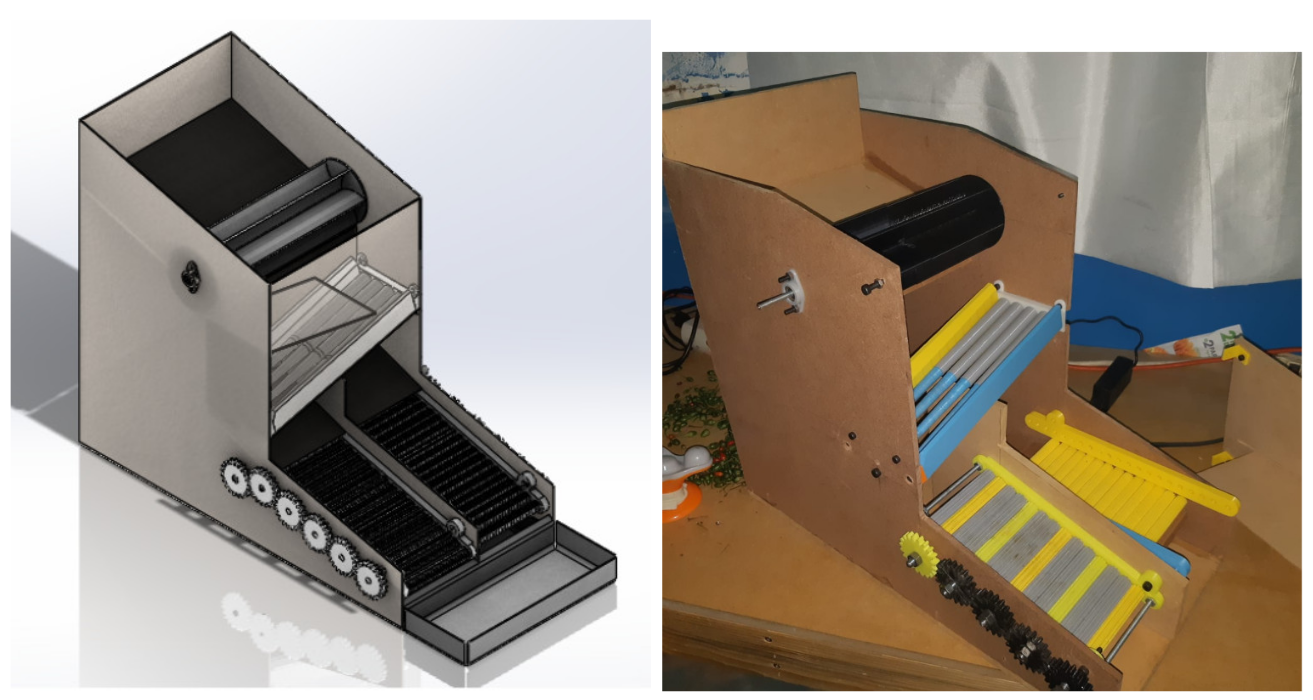
\includegraphics[width=0.98\textwidth]{2022_MaquinaChilePiquin/figs/Prototipo3.png}\\
          \end{tabular}
\end{center}
\end{column} 
\end{columns} 
\end{frame}


\begin{frame}{\citetitle{MarcoNuno_ReporteTecnico2022_B} (5)}
\begin{columns}
\begin{column}{0.70\textwidth}
Prototipo Final:
\begin{itemize}
    \item Actualmente esta en desarrollo, e incluirá los sistemas que funcionaron de los prototipos anteriores
    \item Se incluirá un sensor óptico para medir el rendimiento (cantidad de chiles procesadoss por minuto)
	\end{itemize}
\end{column}
\begin{column}{0.30\textwidth}  
\begin{center}
     \begin{tabular}{c}
         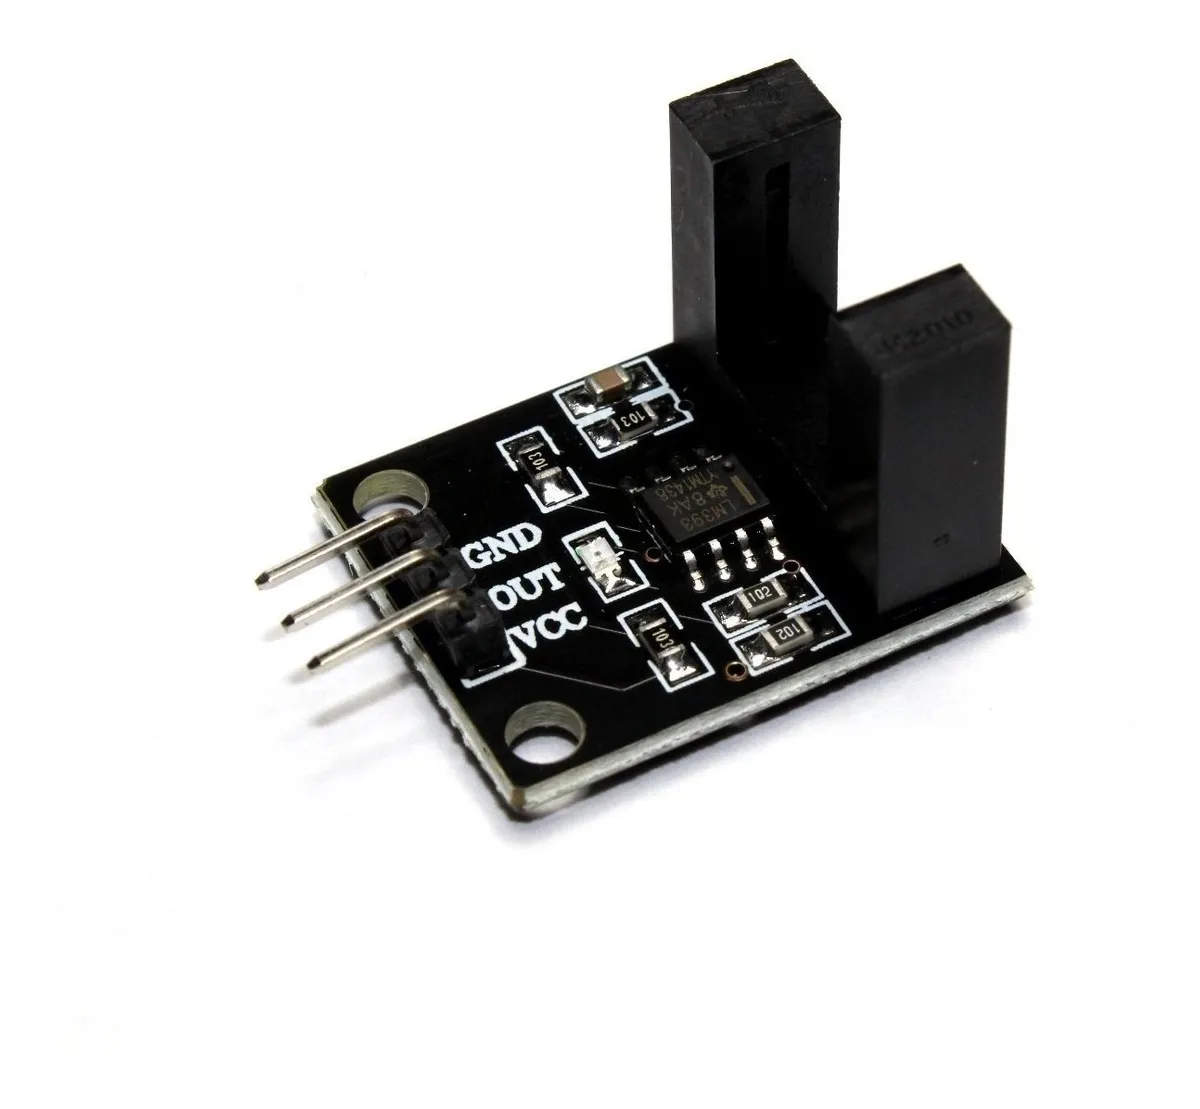
\includegraphics[width=0.98\textwidth]{2022_MaquinaChilePiquin/figs/SensorOptico.png}\\
          \end{tabular}
\end{center}
\end{column} 
\end{columns} 
\end{frame}



%
\renewcommand{\EntradaBibtex}{MarcoNuno_Revista_2022_10_00}

%\begin{frame}{\citetitle{MarcoNuno_Revista_2022_10_00}$^*$ (1)}
\begin{frame}{\citetitle{\EntradaBibtex} \footnotemark[1] (1)}
\begin{columns}
\begin{column}{0.99\textwidth}
	\begin{itemize}  %del cuerpo académico Acuicultura Sustentable (UTMTB-CA-1)
        \item Una aplicación eficaz para uso de transporte publico debe mostrar información acerca de las opciones de movilidad el usuario tiene en una localidad específica.
        \item En algunas localidades, esta información no esta disponible en las aplicaciones de mapas, lo que complica la movilidad del usuario.
		\item Se implementó una App específicamente para Ciudad Victoria, Tamps
	\end{itemize}
\end{column}
%\begin{column}{0.25\textwidth}  
%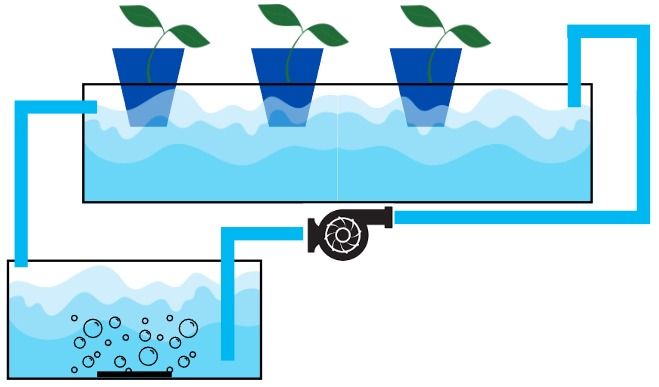
\includegraphics[width=0.98\textwidth]{2022_HidroponicosDavid/figs/dft}
%\end{column}
%\begin{column}{0.25\textwidth}
%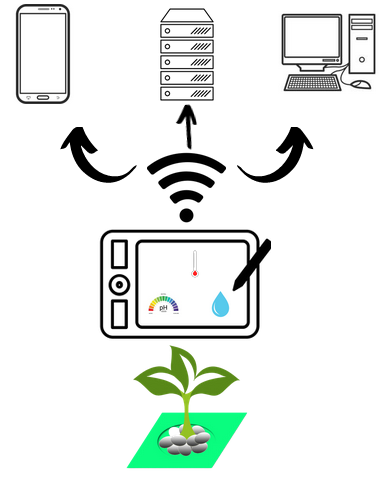
\includegraphics[width=0.98\textwidth]{2022_HidroponicosDavid/figs/iot}
%\end{column}
\end{columns} 
\footnotetext[1]{\fullcite{\EntradaBibtex}}
\end{frame}


\begin{frame}{\citetitle{\EntradaBibtex} (2)}
\begin{columns}
\begin{column}{0.25\textwidth}  
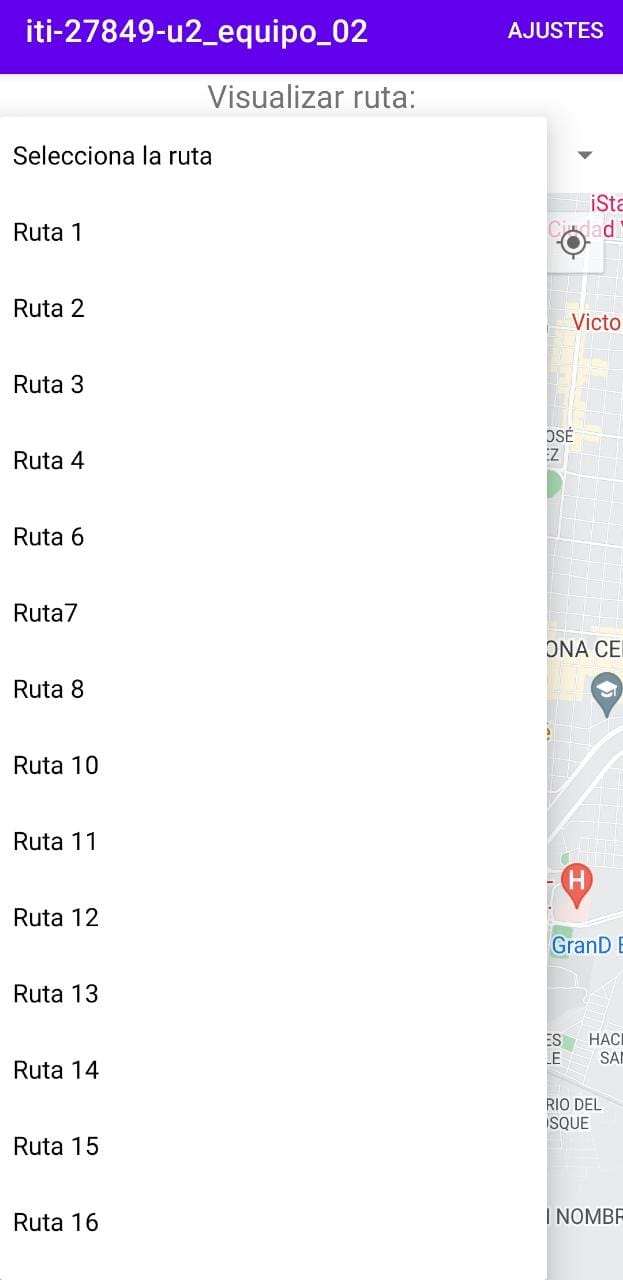
\includegraphics[width=0.82\textwidth]{2022_MapaVickyRanch/figs/F3}
\end{column}
\begin{column}{0.25\textwidth}  
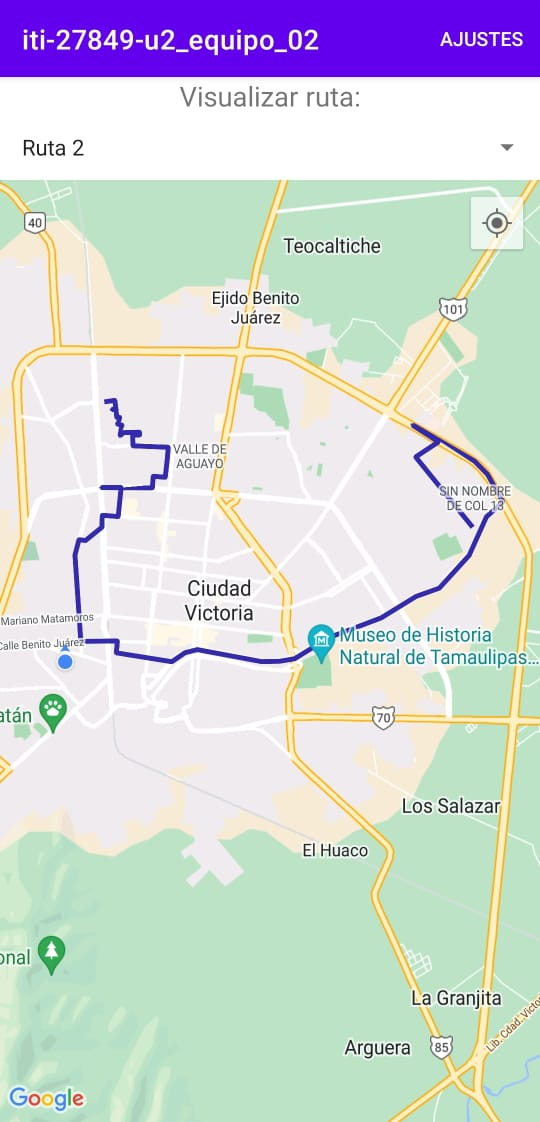
\includegraphics[width=0.82\textwidth]{2022_MapaVickyRanch/figs/F4}
\end{column}
\begin{column}{0.25\textwidth}  
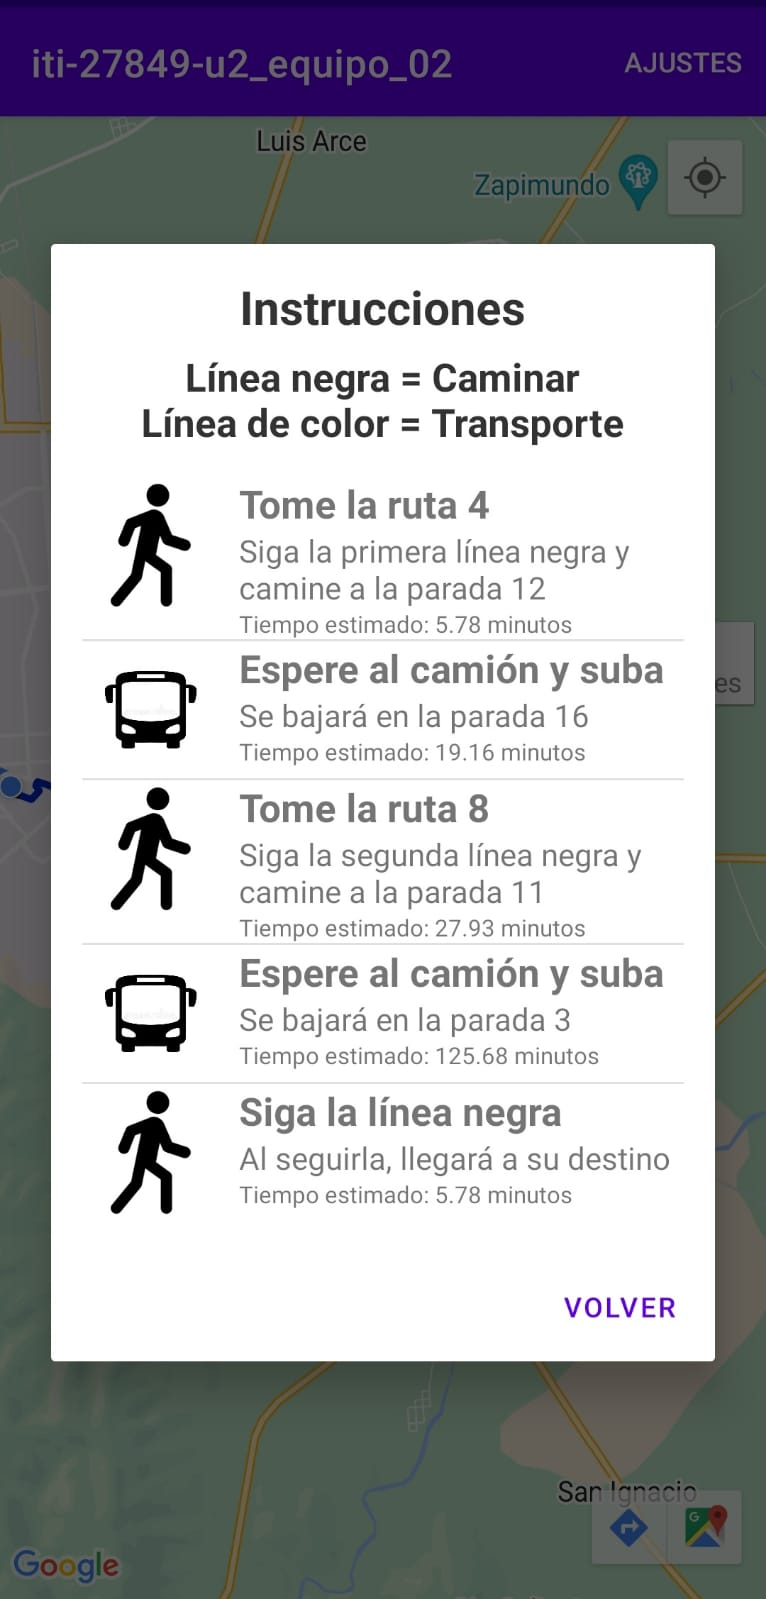
\includegraphics[width=0.82\textwidth]{2022_MapaVickyRanch/figs/F9}
\end{column}
\begin{column}{0.25\textwidth}  
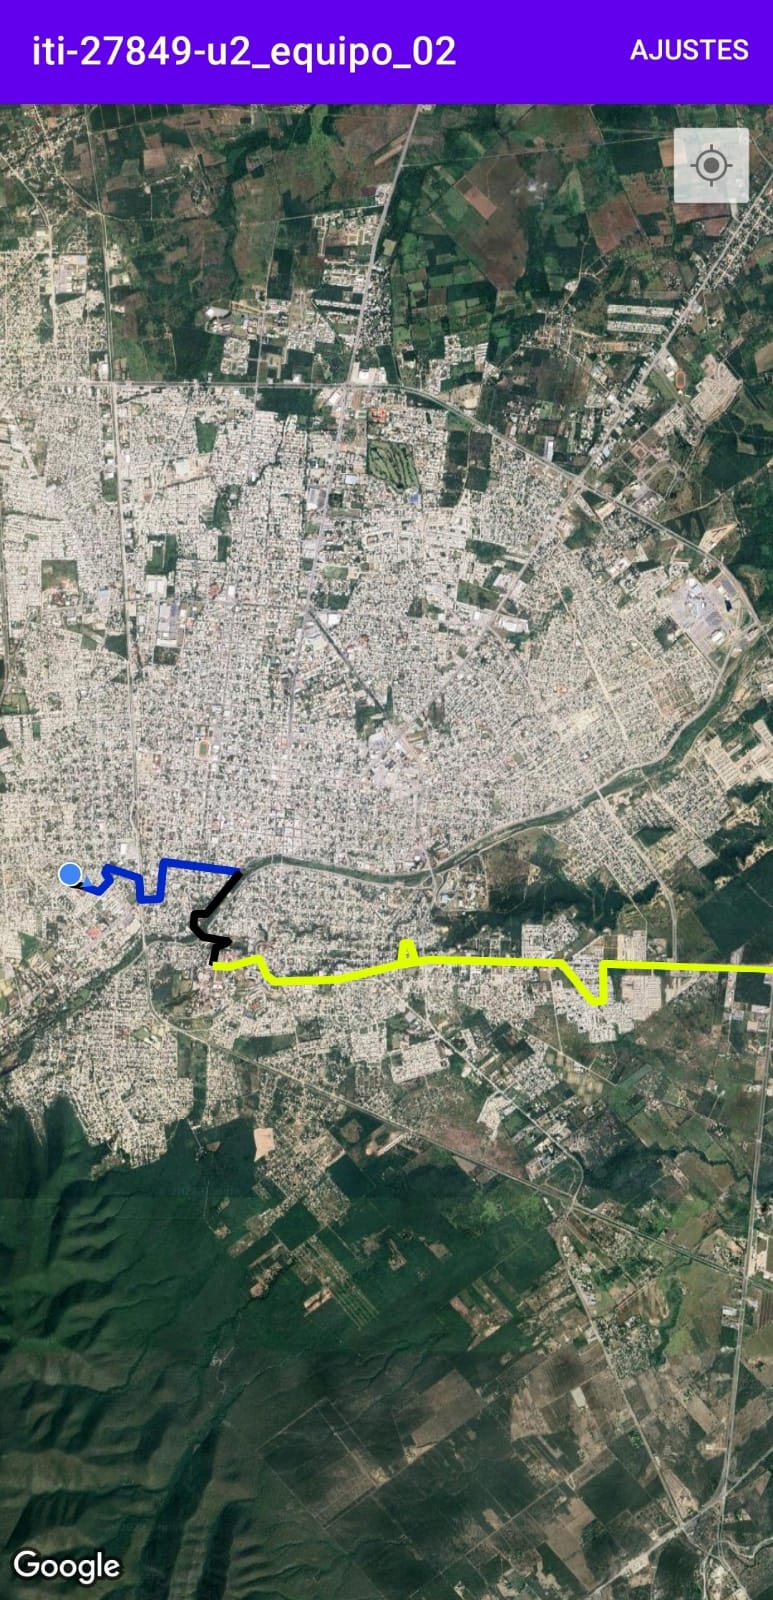
\includegraphics[width=0.82\textwidth]{2022_MapaVickyRanch/figs/F13}
\end{column}

\end{columns} 
\end{frame}


%
\renewcommand{\EntradaBibtex}{MapaRealidadVirtual_UPV_2022}
						 
\begin{frame}{\citetitle{\EntradaBibtex} \footnotemark[1] (1)}
\begin{columns}
\begin{column}{0.99\textwidth}
	\begin{itemize}
		\item Se propone una aplicación de RA que despliegue un MAPA de la UPV
		\item Se generó el modelo utilizando Blender y se exportó a un formato GLB
		\item La aplicación hace uso de la cámara para desplegar el modelo en una superficie con textura
	\end{itemize}
\end{column}
\begin{column}{0.01\textwidth}  
\begin{center}
     \begin{tabular}{c}
%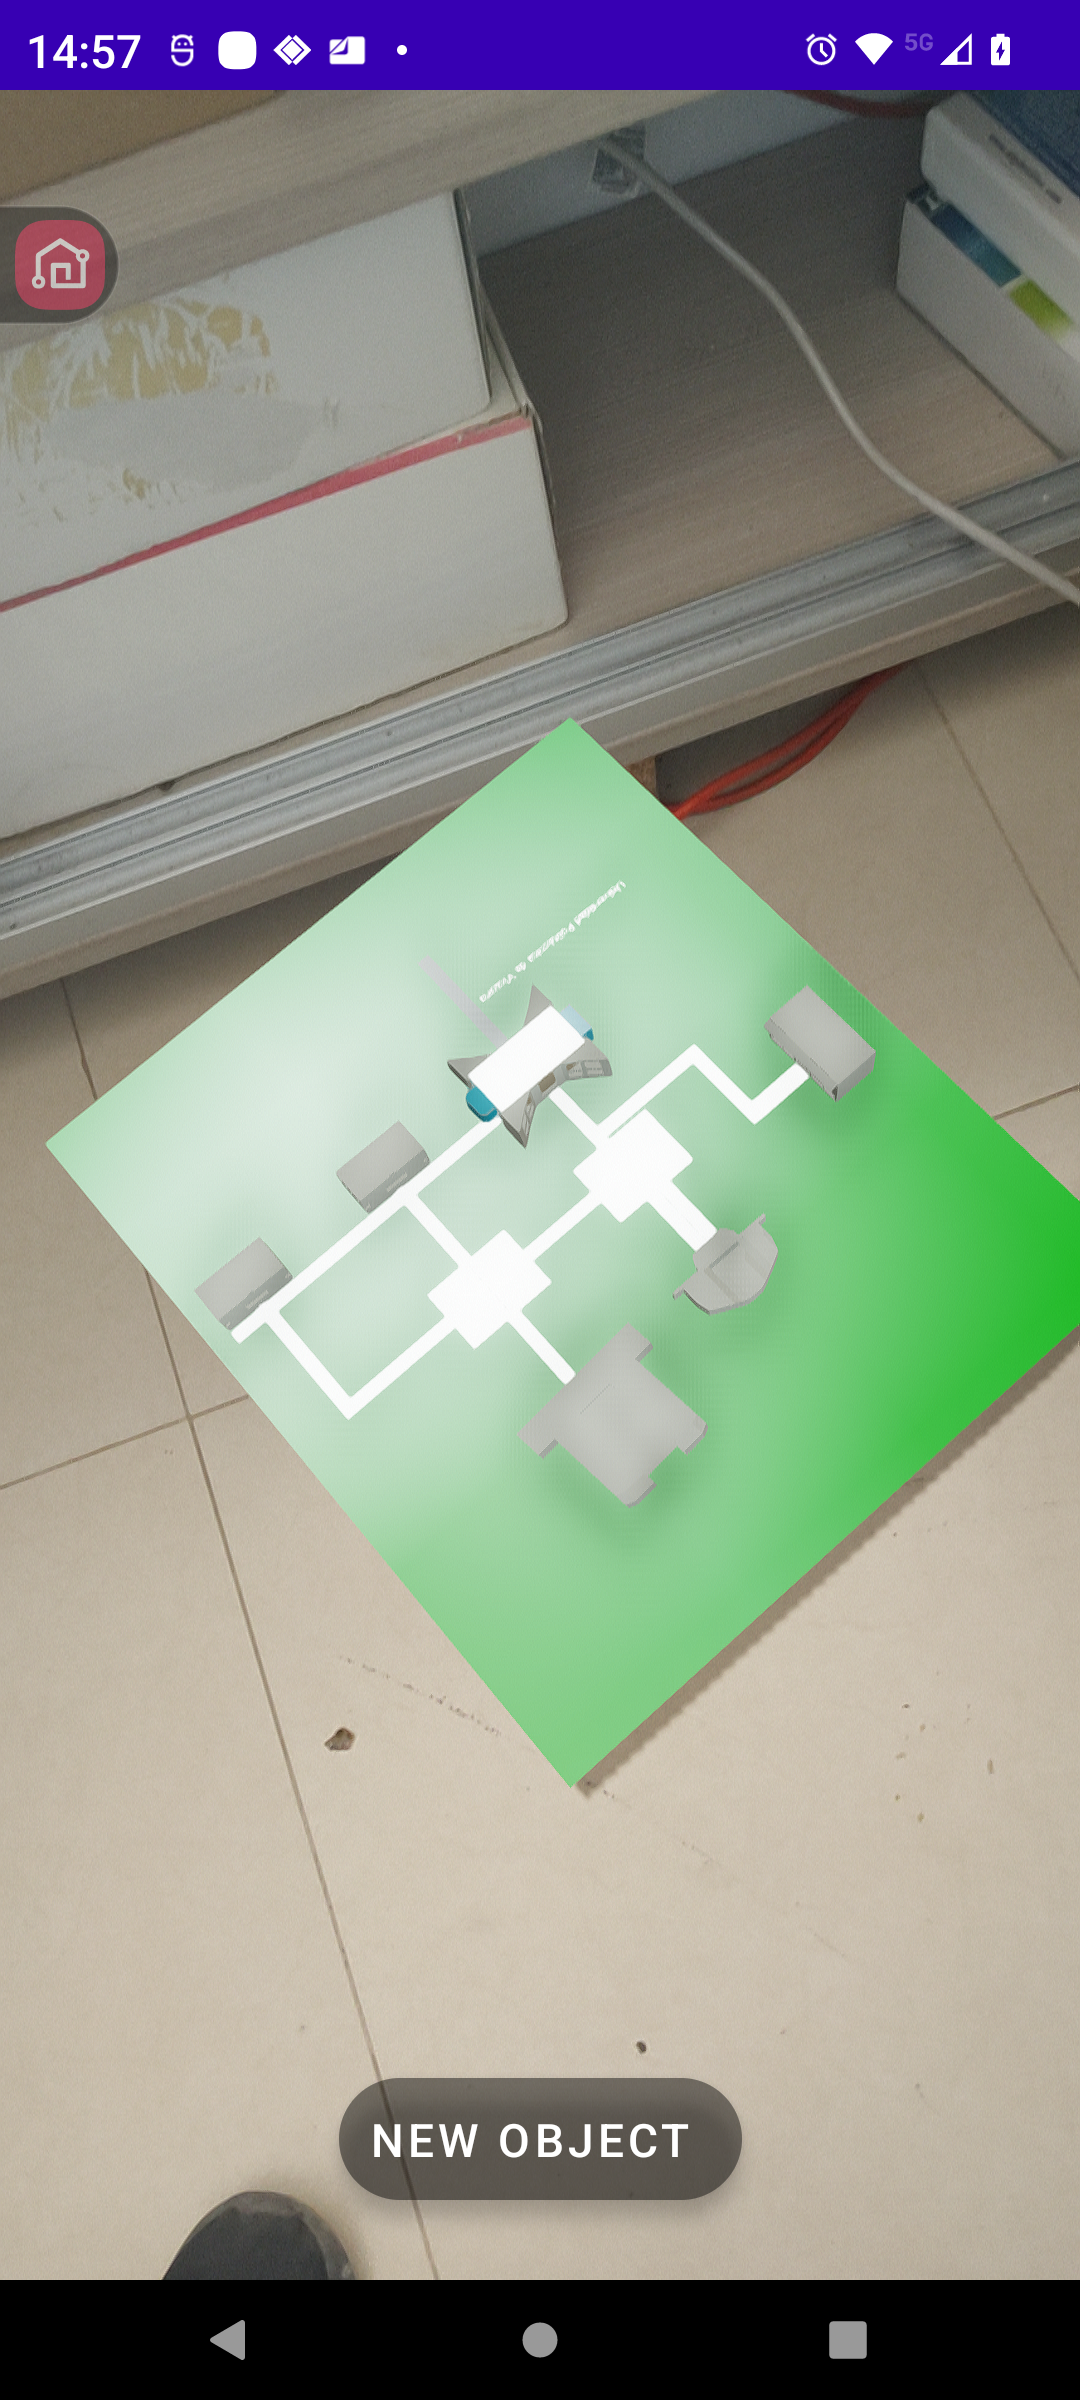
\includegraphics[width=0.48\textwidth]{2022_MapaUPV_RealidadAumentada/figs/MapaUPV_01}
%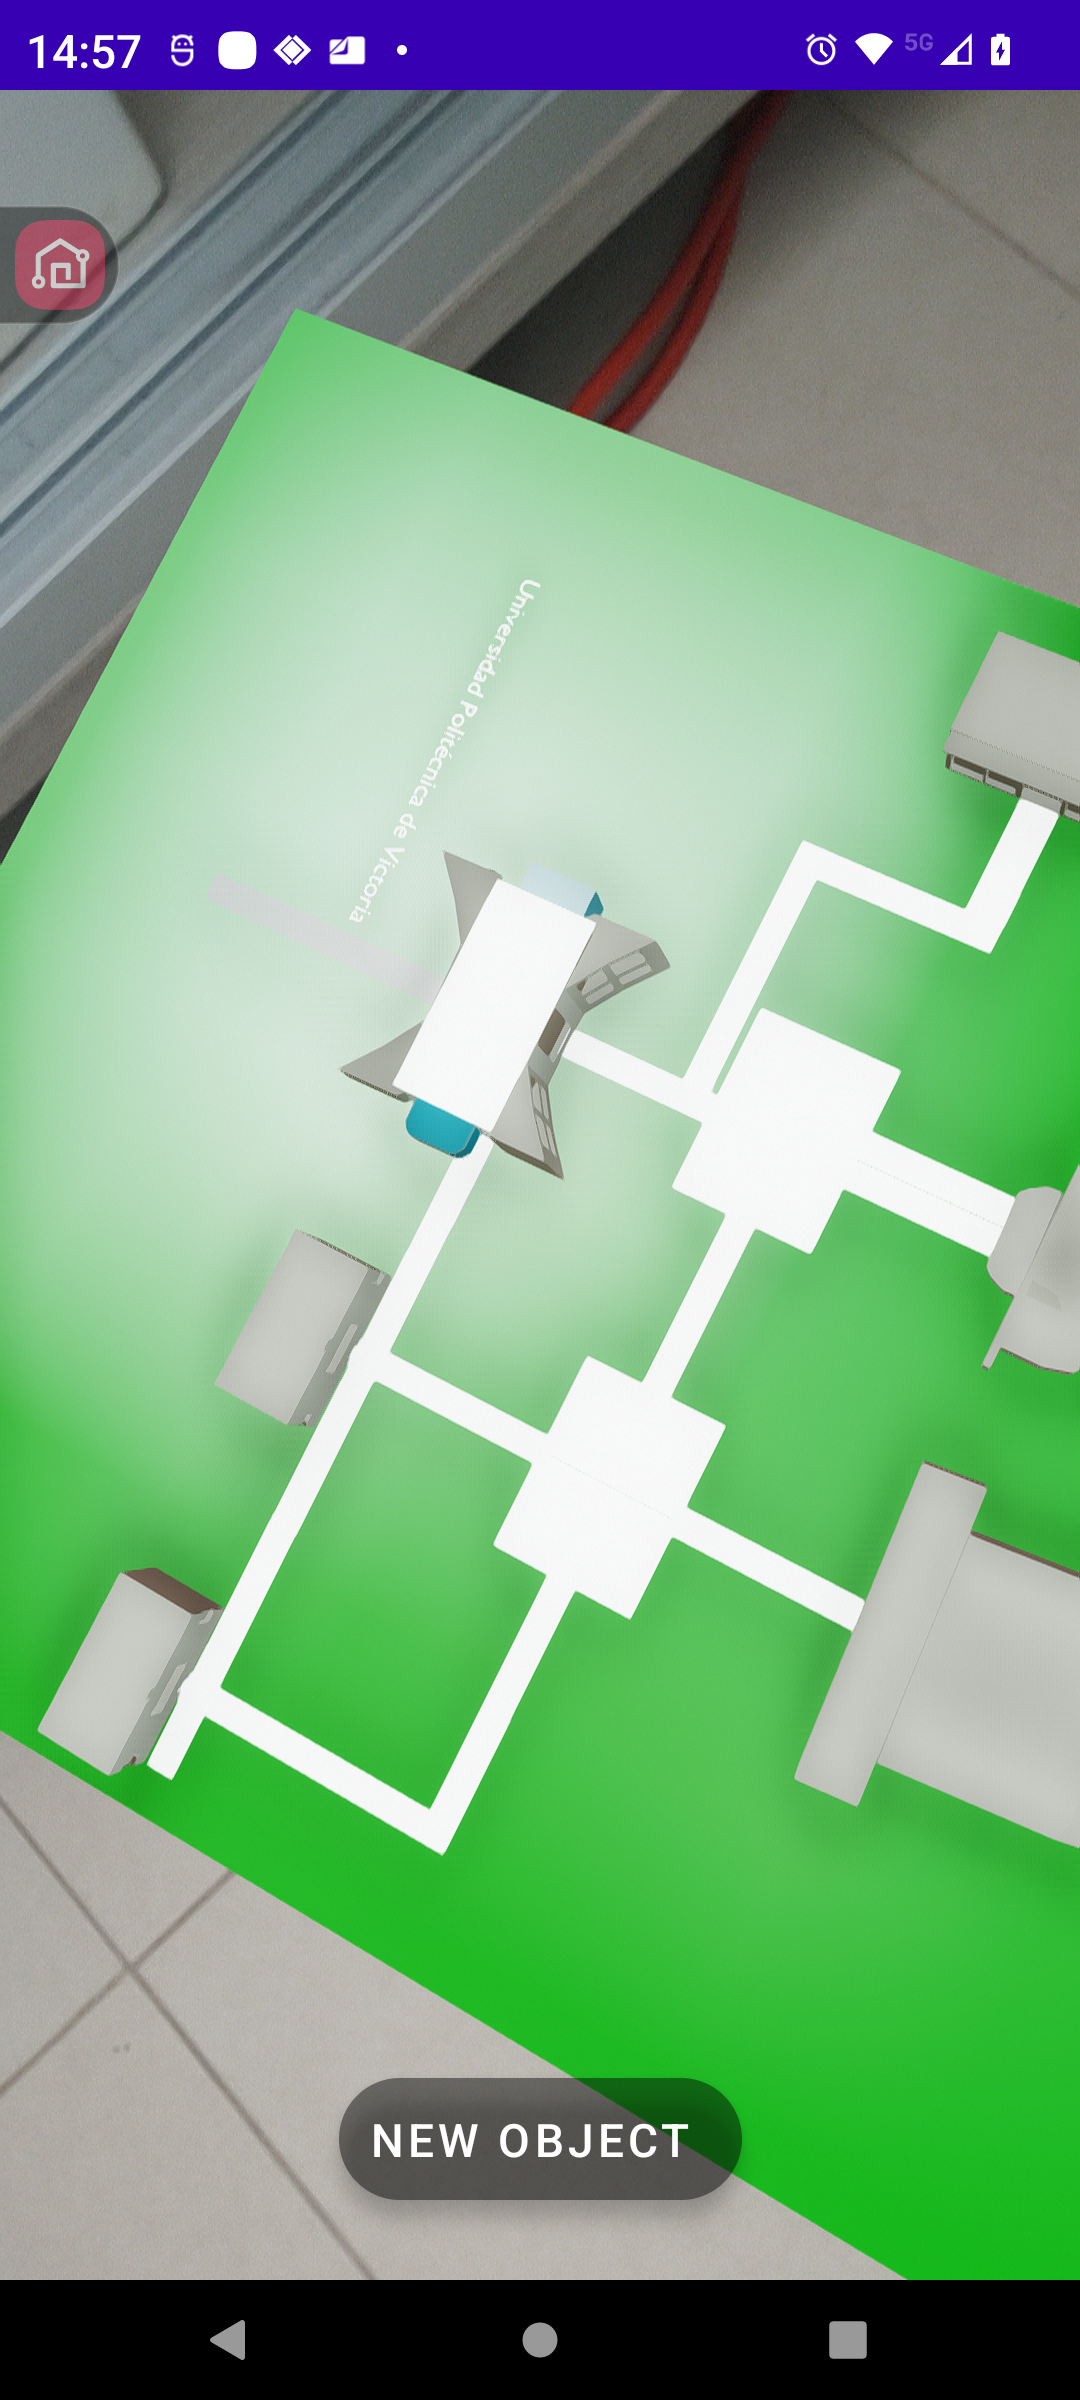
\includegraphics[width=0.48\textwidth]{2022_MapaUPV_RealidadAumentada/figs/MapaUPV_02}\\         
      \end{tabular}
\end{center}
\end{column} 
\end{columns} 
\footnotetext[1]{\fullcite{\EntradaBibtex}}
\end{frame}


\begin{frame}{\citetitle{\EntradaBibtex} (2)}
\begin{columns}
\begin{column}{0.4\textwidth}
	\begin{itemize}
		\item Se propone una aplicación de RA que despliegue un MAPA de la UPV
	\end{itemize}
\end{column}
\begin{column}{0.6\textwidth}  
\begin{center}
     \begin{tabular}{c}
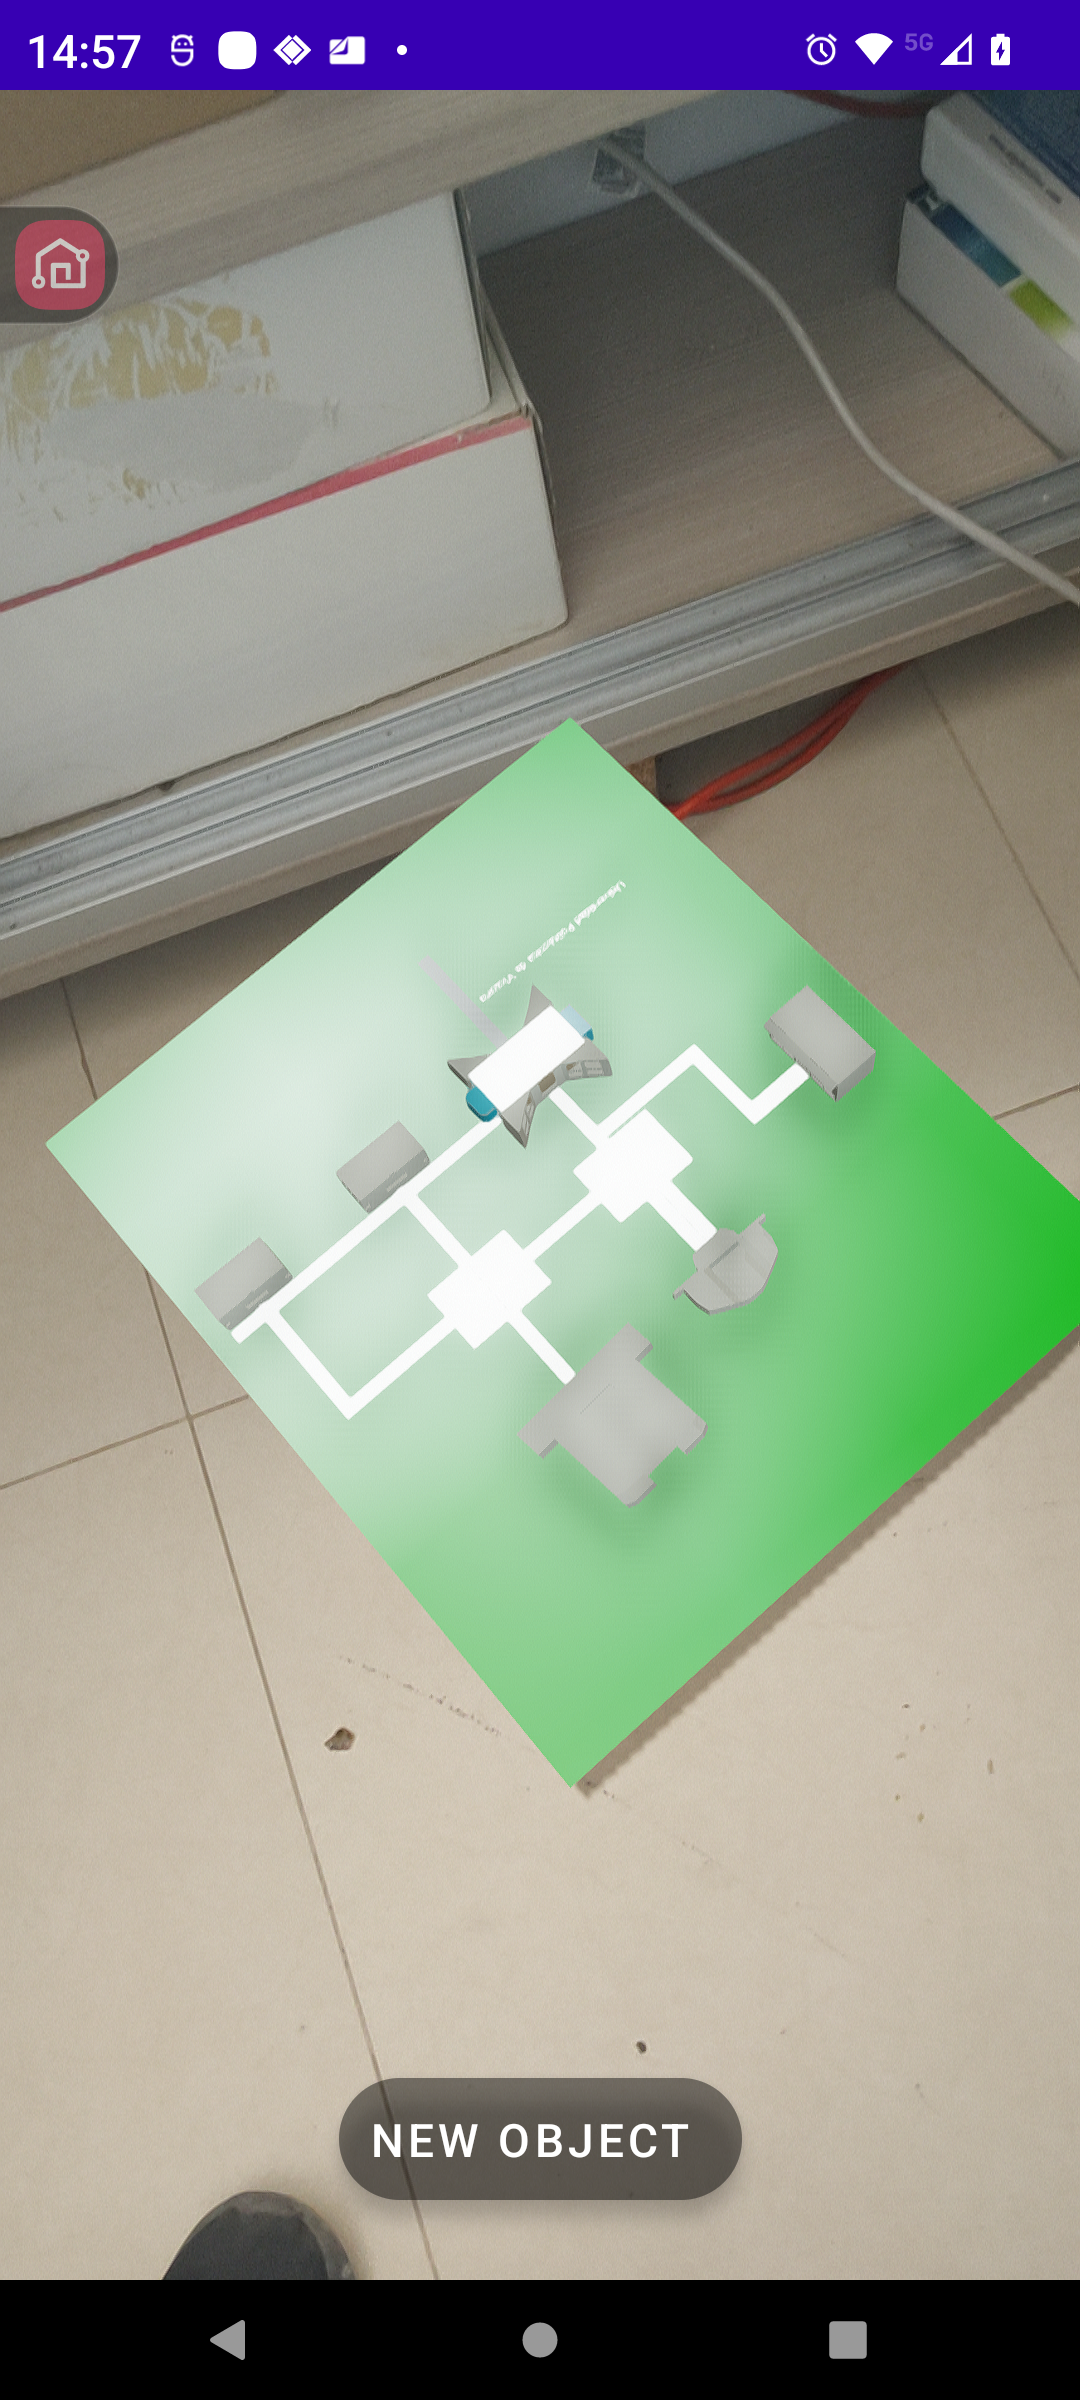
\includegraphics[width=0.24\textwidth]{2022_MapaUPV_RealidadAumentada/figs/MapaUPV_01}
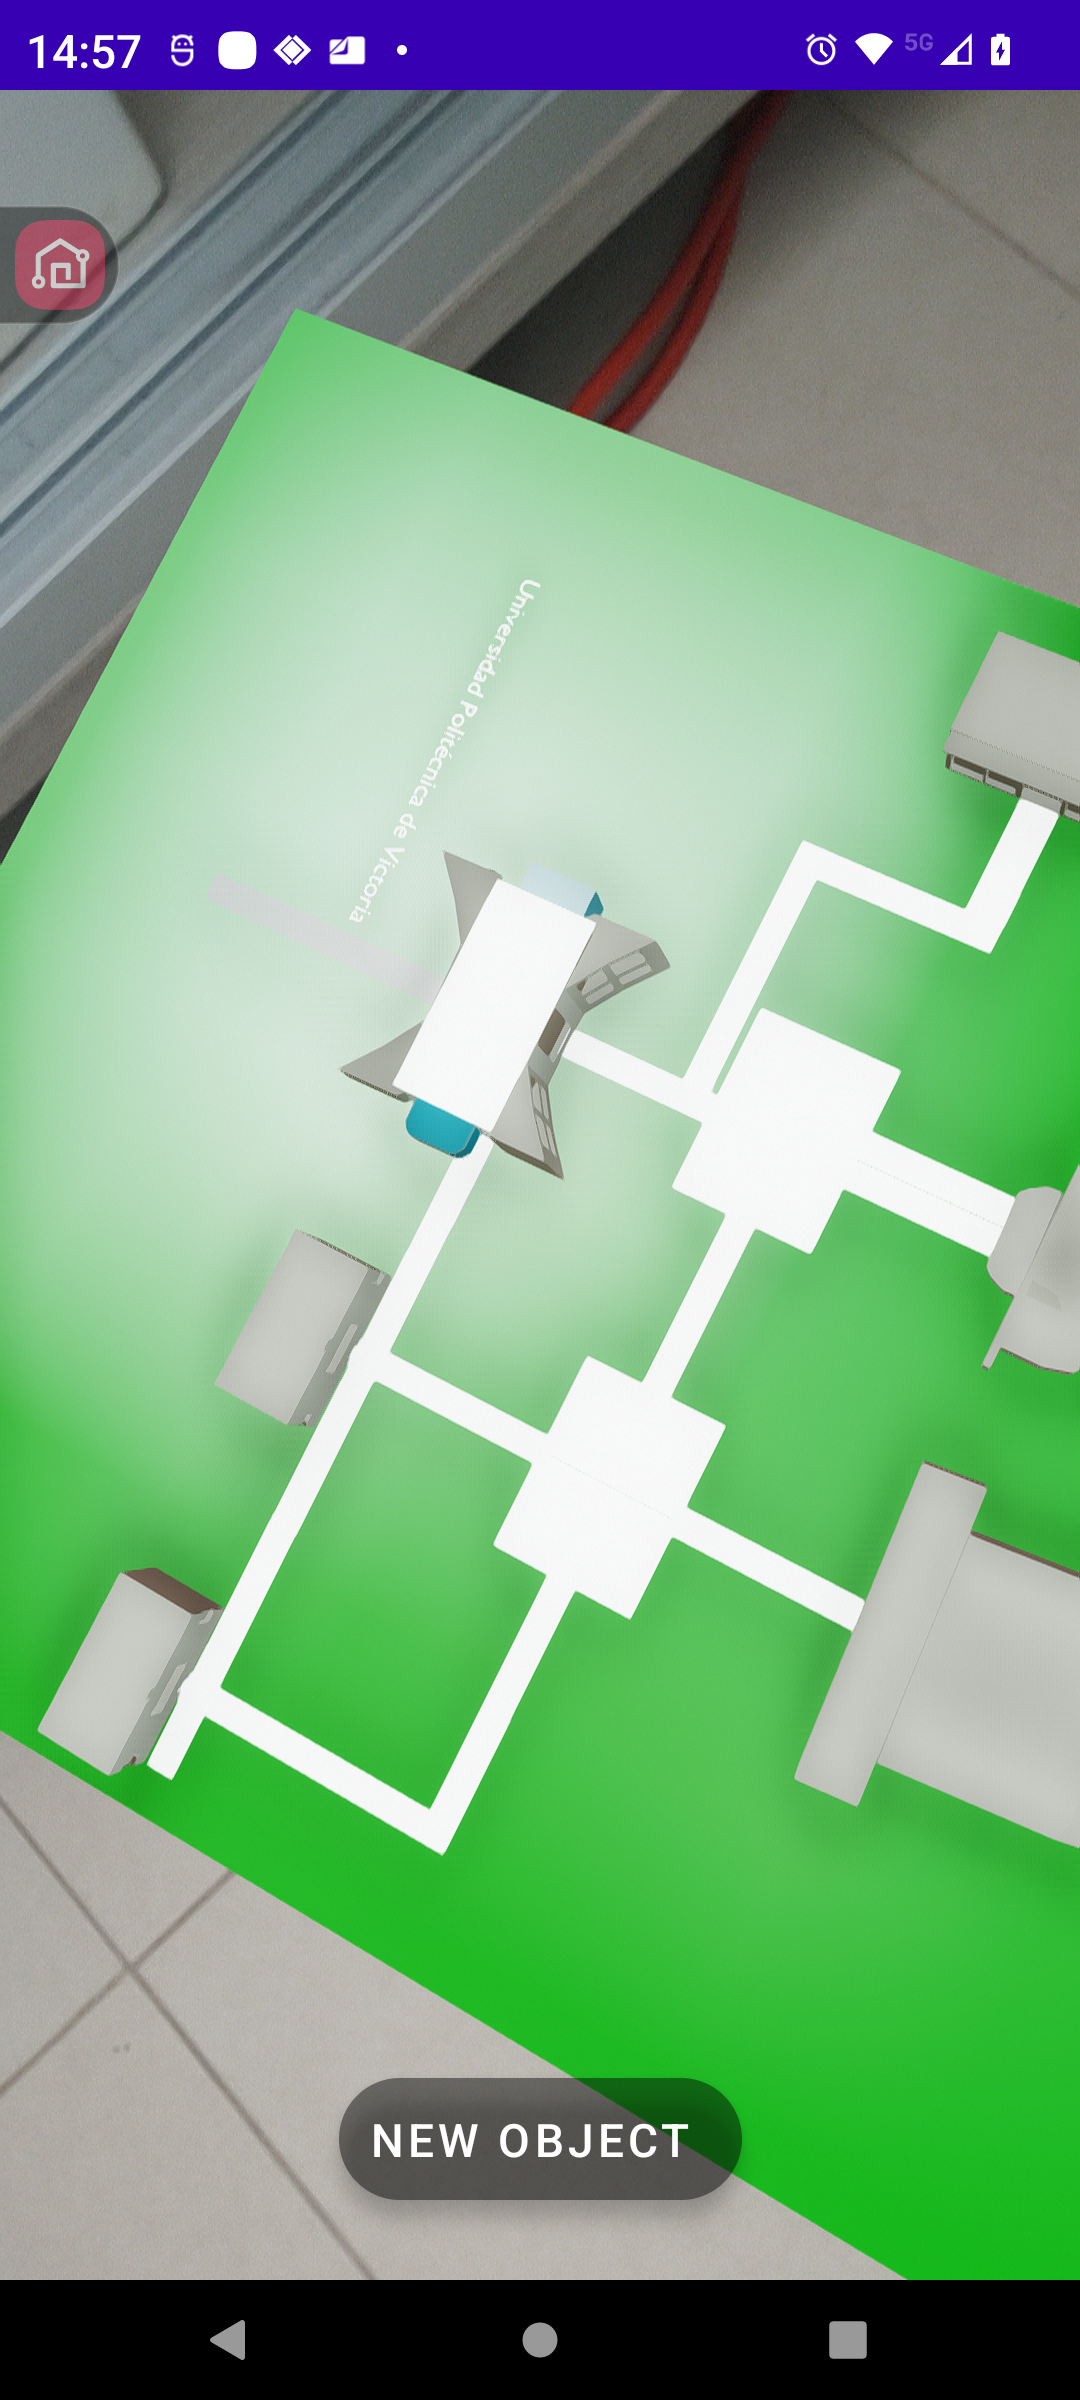
\includegraphics[width=0.24\textwidth]{2022_MapaUPV_RealidadAumentada/figs/MapaUPV_02}
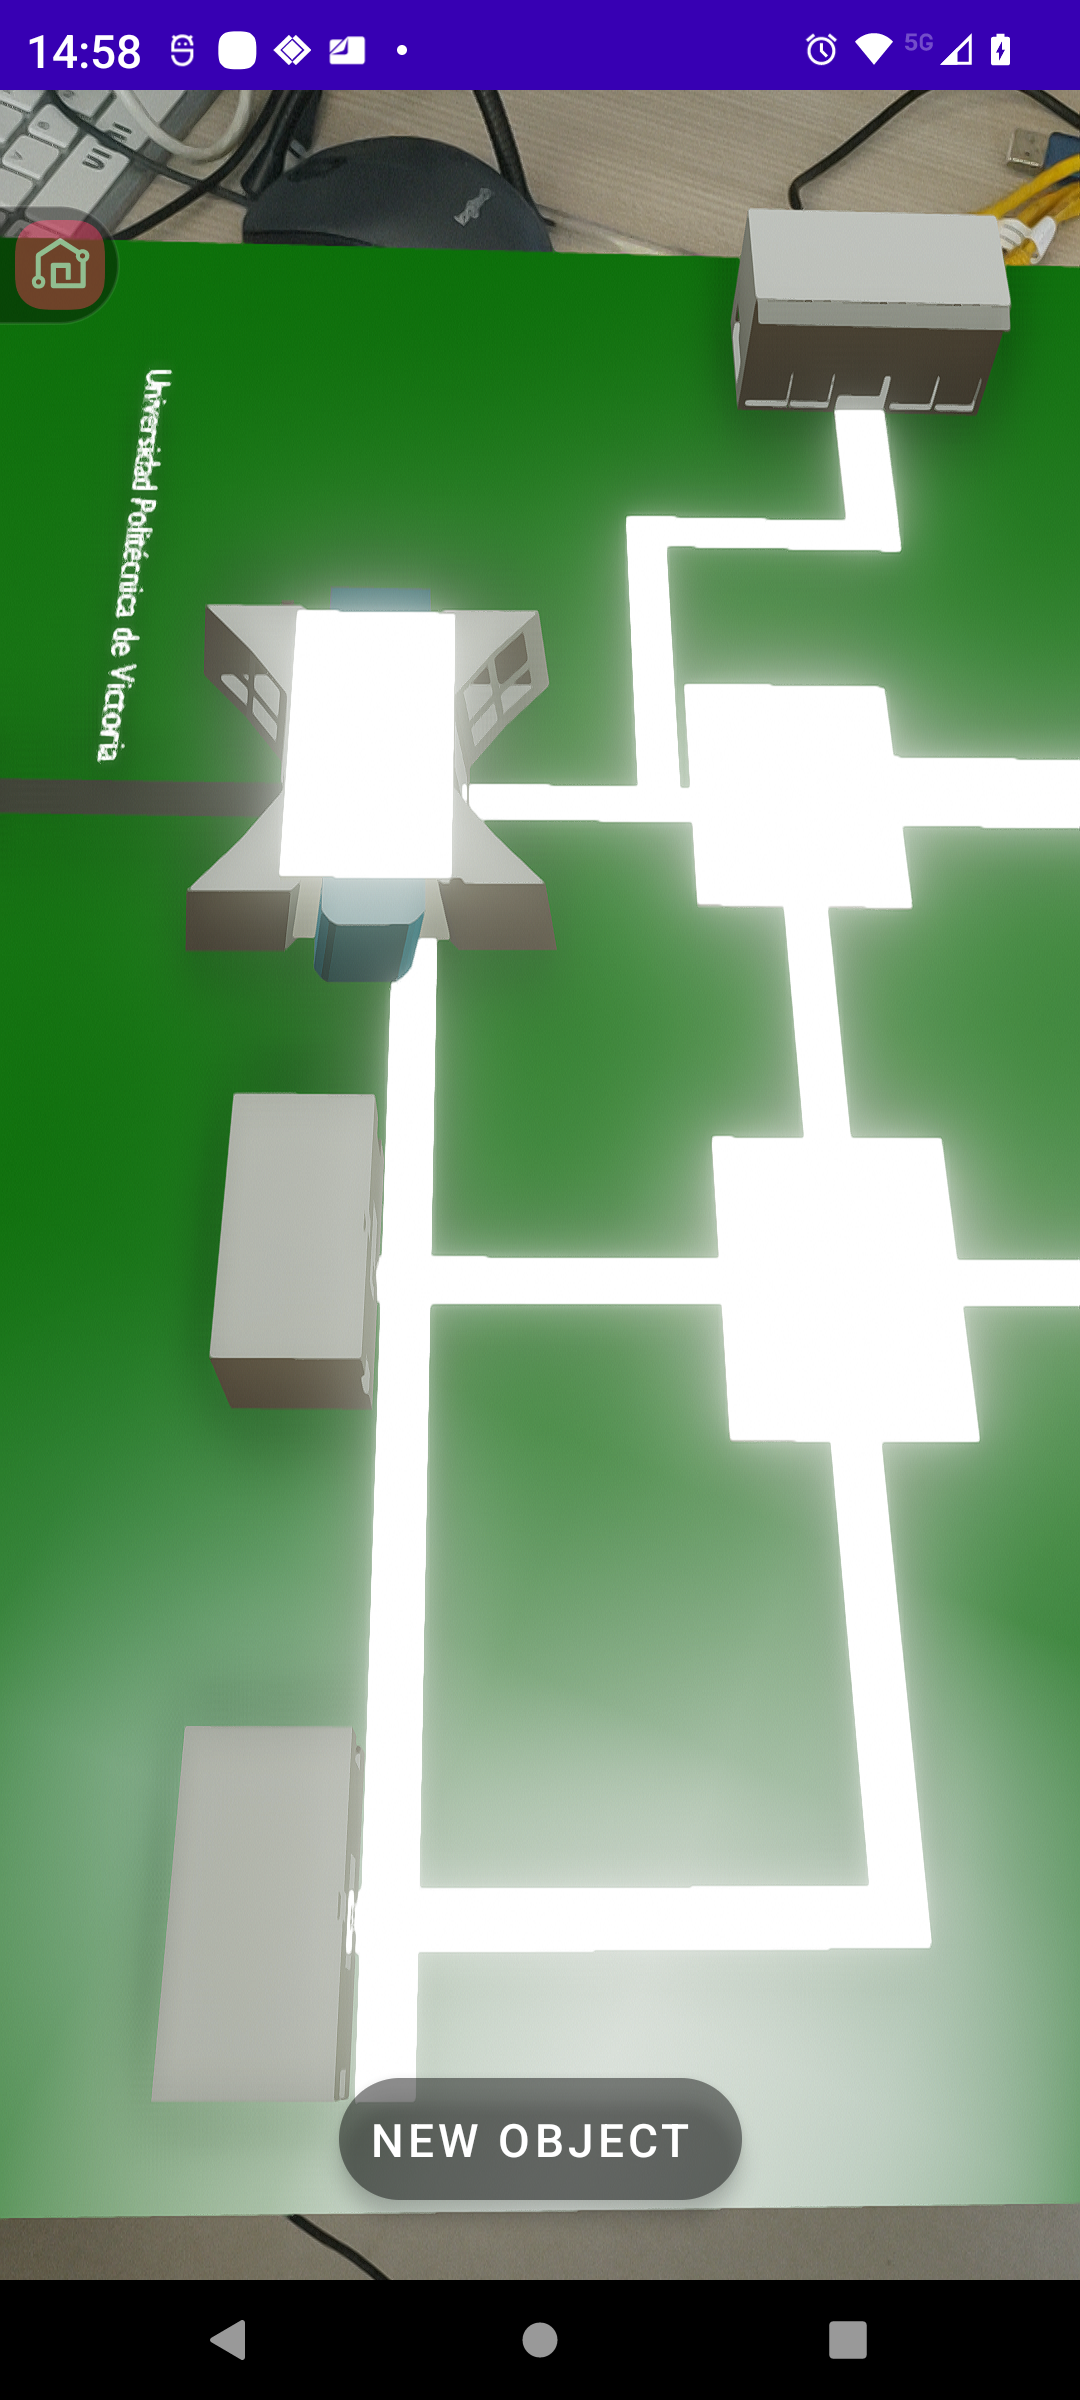
\includegraphics[width=0.24\textwidth]{2022_MapaUPV_RealidadAumentada/figs/MapaUPV_03}
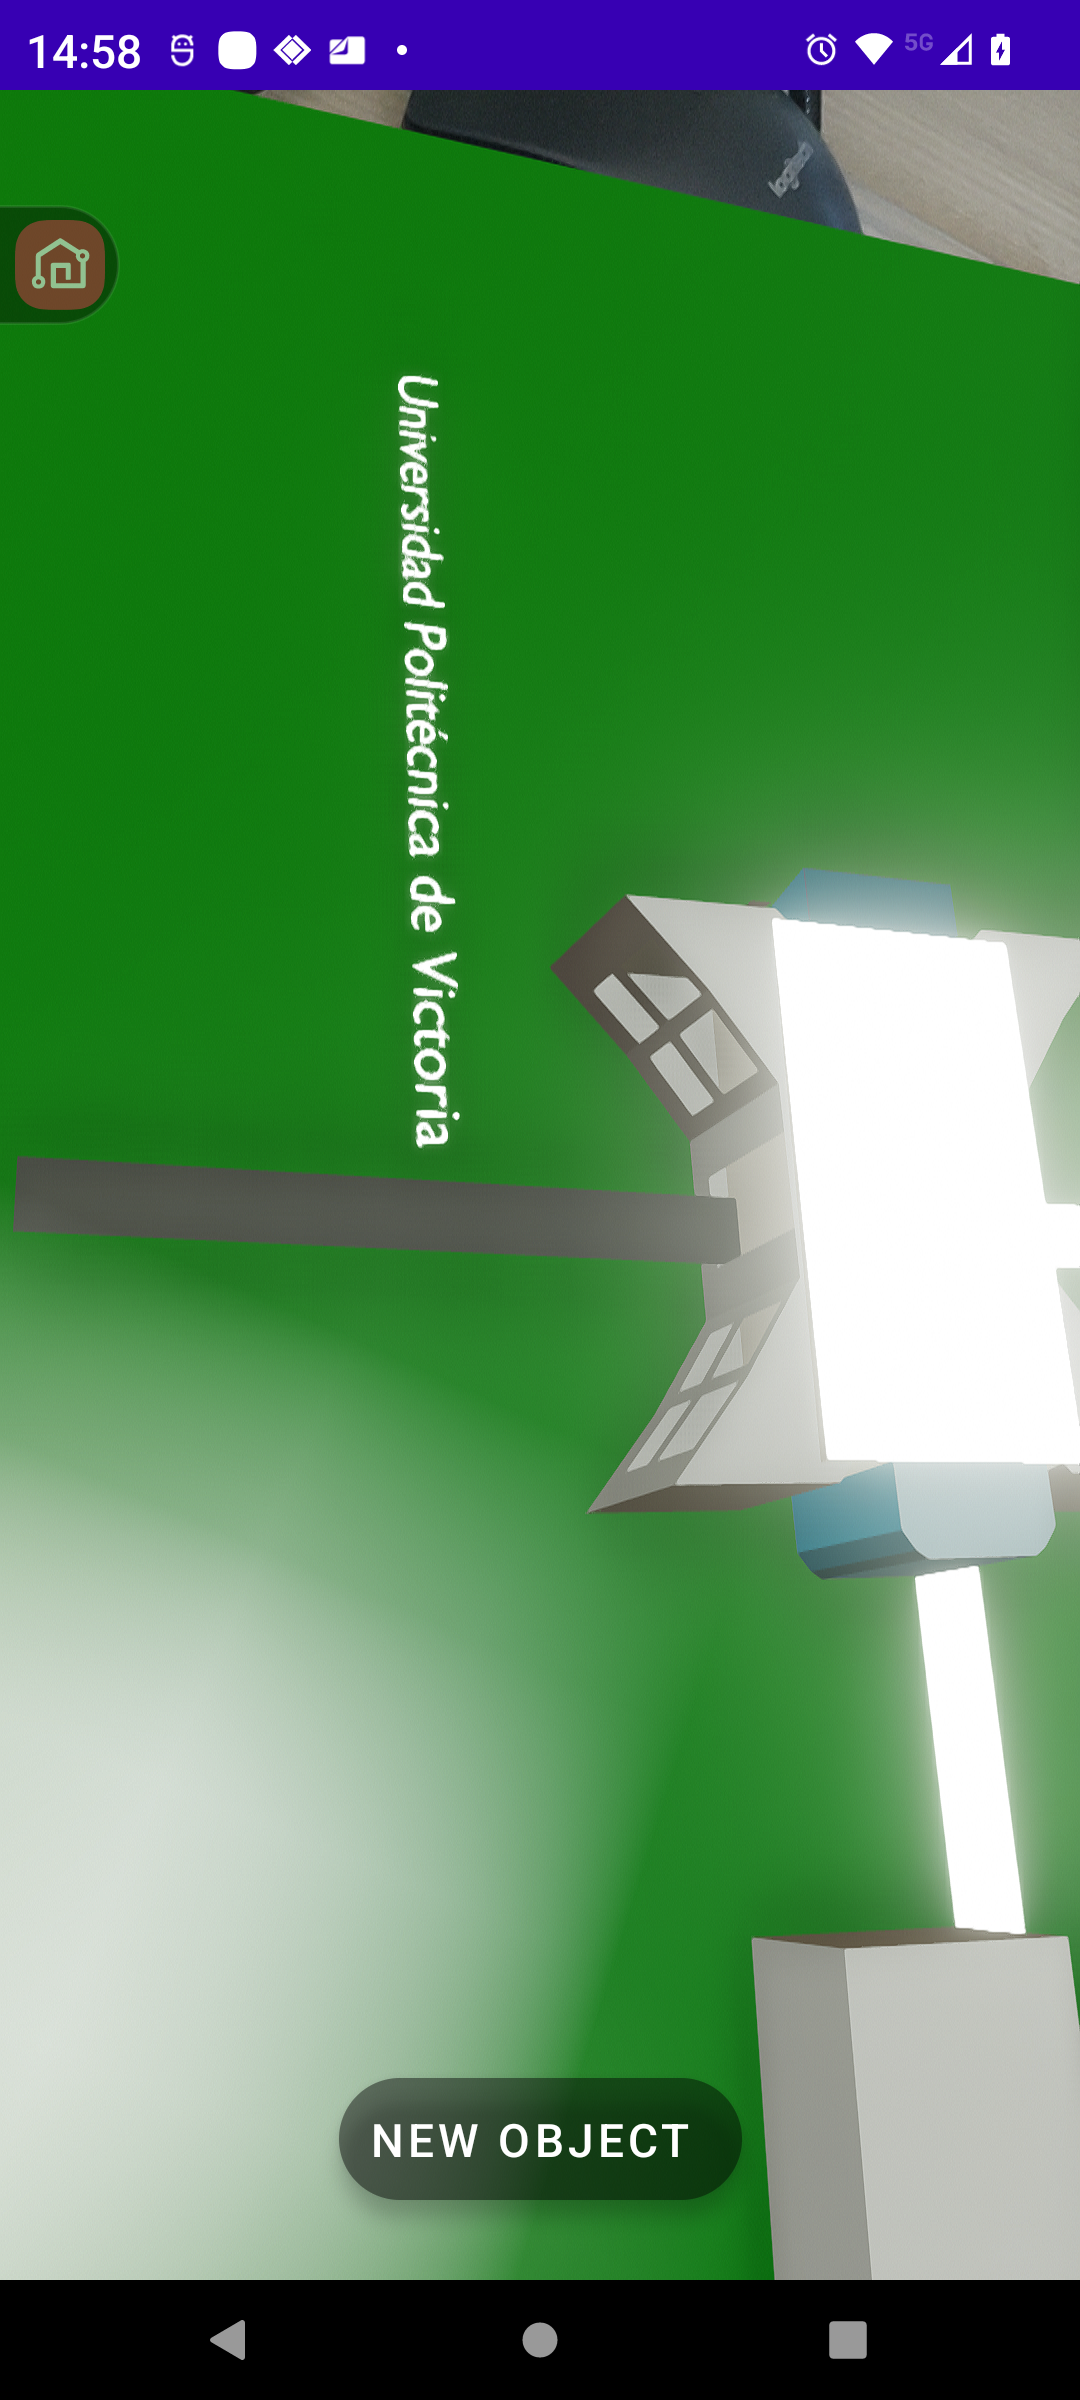
\includegraphics[width=0.24\textwidth]{2022_MapaUPV_RealidadAumentada/figs/MapaUPV_04}\\         
      \end{tabular}
\end{center}
\end{column} 
\end{columns} 

\end{frame}






%\renewcommand{\EntradaBibtex}{ArticuloDavidHidroponia_2022}


\begin{frame}{\citetitle{\EntradaBibtex} \footnotemark[1] (1)}
\begin{columns}
\begin{column}{0.75\textwidth}
	\begin{itemize}  %del cuerpo académico Acuicultura Sustentable (UTMTB-CA-1)
        \item Los sistemas hidropónicos se basan en el cultivo de plantas sin la necesidad del suelo
        \item Las necesidades nutricionales de las plantas a cultivar son suministrandas a sus raíces mediante una solución nutritiva
		\item Se implementó un sistema hidropónico tipo DFT (Deep Flow Technique)
		\item Se trabaja en la incorporación de un monitoreo remoto para dicho sistema, con alarmas y notificaciones
	\end{itemize}
\end{column}
\begin{column}{0.25\textwidth}  
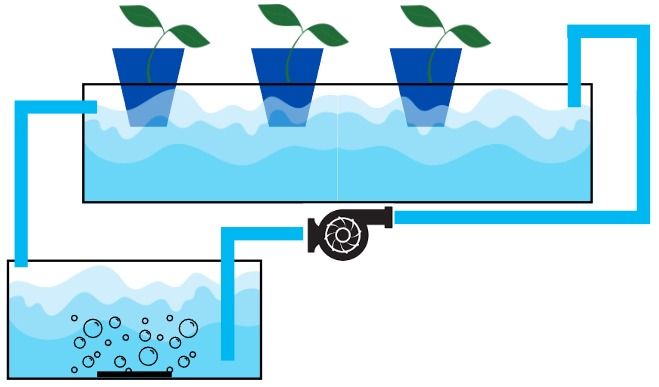
\includegraphics[width=0.98\textwidth]{2022_HidroponicosDavid/figs/dft}
\end{column}
%\begin{column}{0.25\textwidth}
%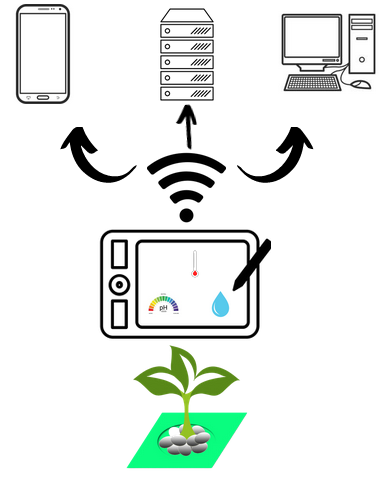
\includegraphics[width=0.98\textwidth]{2022_HidroponicosDavid/figs/iot}
%\end{column}
\end{columns} 
\footnotetext[1]{\fullcite{\EntradaBibtex}}
\end{frame}


\begin{frame}{\citetitle{\EntradaBibtex} (2)}
\begin{columns}
\begin{column}{0.35\textwidth}
Componentes:
\begin{itemize}
        \item Raspberry Pi 3 B+ y módulo ESP32
        \item Sensores de temperatura, humedad, pH, conductividad eléctrica
        \item Bomba periférica de 1/2 HP y bombas peristálticas        
        \item Tubos de PVC
	\end{itemize}
\end{column}
\begin{column}{0.35\textwidth}  
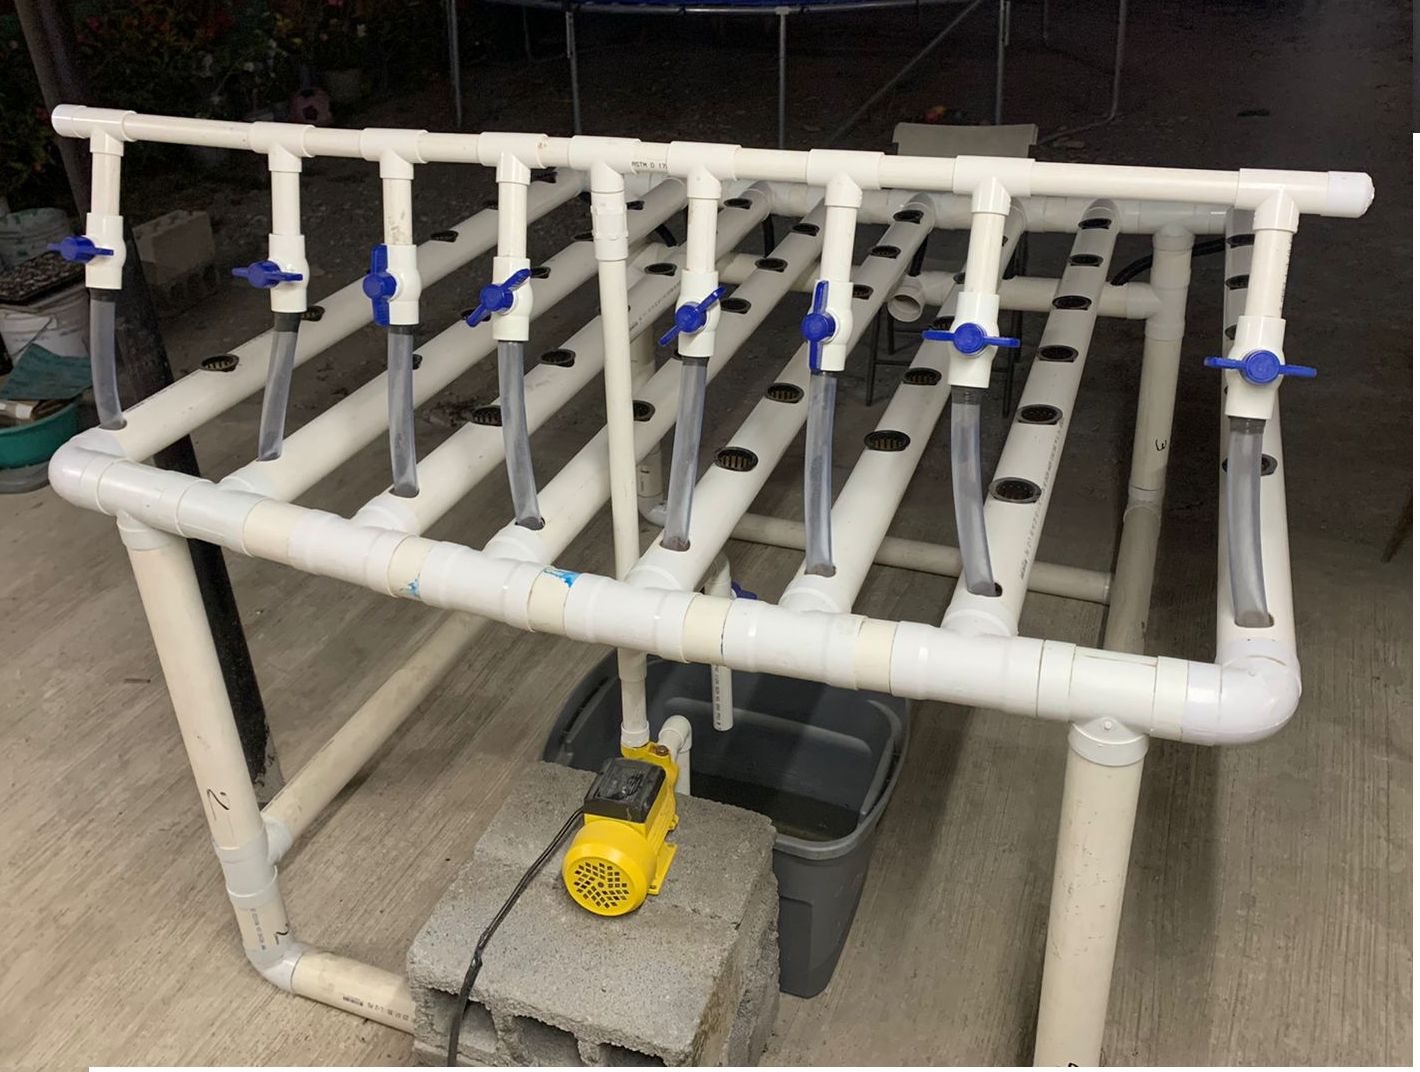
\includegraphics[width=0.98\textwidth]{2022_HidroponicosDavid/figs/1}
\end{column}
\begin{column}{0.30\textwidth}  
\includegraphics[width=0.98\textwidth]{2022_HidroponicosDavid/figs/Circuito_Articulo}
\end{column}
\end{columns} 
\end{frame}

\begin{frame}{\citetitle{\EntradaBibtex} (3)}
\begin{columns}
\begin{column}{0.30\textwidth}
\begin{itemize}
		\item Se utiliza la plataforma Node-Red para visualizar las lecturas de los sensores
	\end{itemize}
\end{column}
\begin{column}{0.20\textwidth}  
         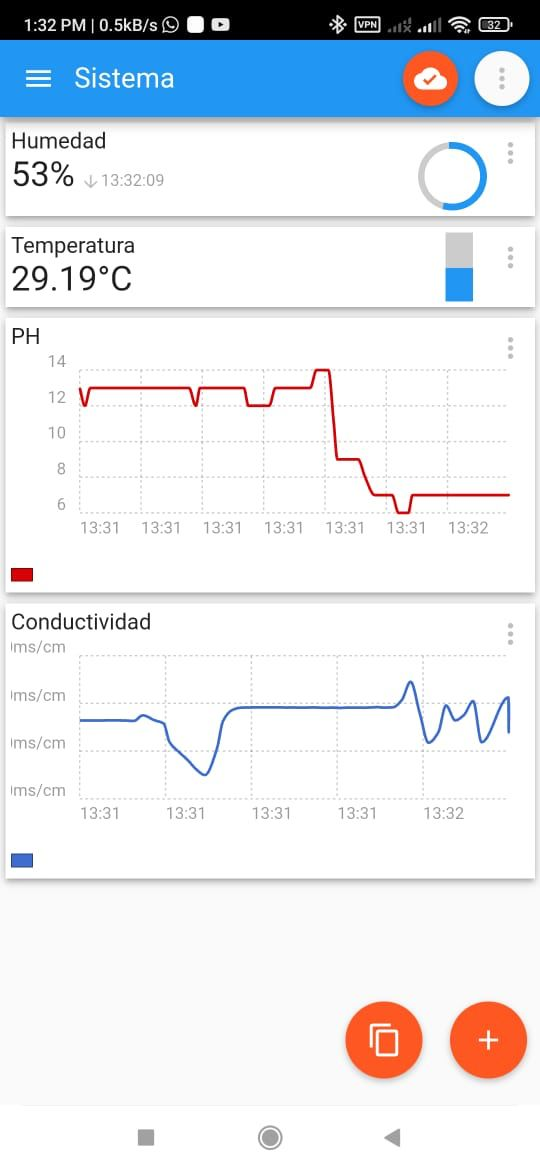
\includegraphics[width=0.98\textwidth]{2022_HidroponicosDavid/figs/app}

\end{column} 
\begin{column}{0.50\textwidth}  
         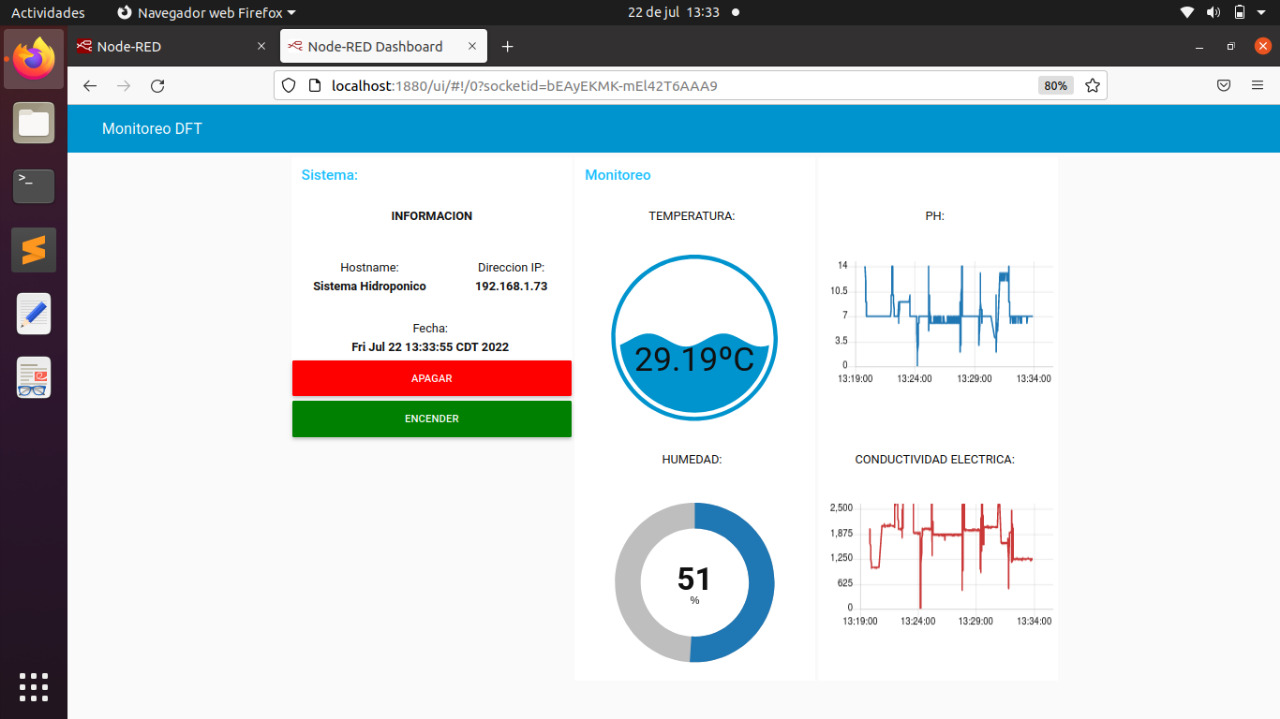
\includegraphics[width=0.98\textwidth]{2022_HidroponicosDavid/figs/servidor}
\end{column} 
\end{columns} 
\end{frame}







%\renewcommand{\EntradaBibtex}{Avatar3d_Echartea_2021}



\begin{frame}{\citetitle{\EntradaBibtex} \footnotemark[1] (1)}
%\begin{block}{Aplicación Movil para Concientizar a Niños Acerca del Cuidado del Peso (1)} 
	\begin{itemize}
\item Se requieren herramientas que apoyen en la concientización de problemas médicos graves (Obesidad)
\item Se integra una aplicación móvil que muestre un avatar tridimensional cuyo peso, estatura y edad sea configurable con por usuario
\item Es posible configurar el numero de comidas y el tipo de ejercicio de la simulación
\item Al finalizar la simulación, la aplicación mostrará el antes o despues basado en en los IMCs y los parametros del avatar. 
\item Herramientas utilizadas
	\begin{itemize}
		\item Unity
		\item MakeHuman 
	\end{itemize}
	\end{itemize}
%\end{block} 
\footnotetext[1]{\fullcite{\EntradaBibtex}}
\end{frame}

\begin{frame}{\citetitle{\EntradaBibtex} (2)}
%\begin{block}{Simulación de modelo de diabetes en un dispositivo móvil (2)} 
\begin{center}
     \begin{tabular}{ccc}
         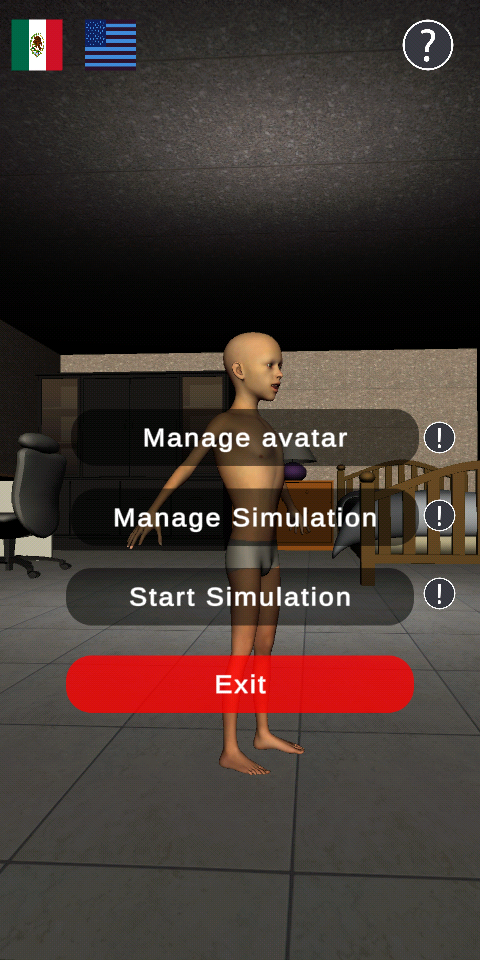
\includegraphics[width=0.25\textwidth]{Figs/Echartea1}&
         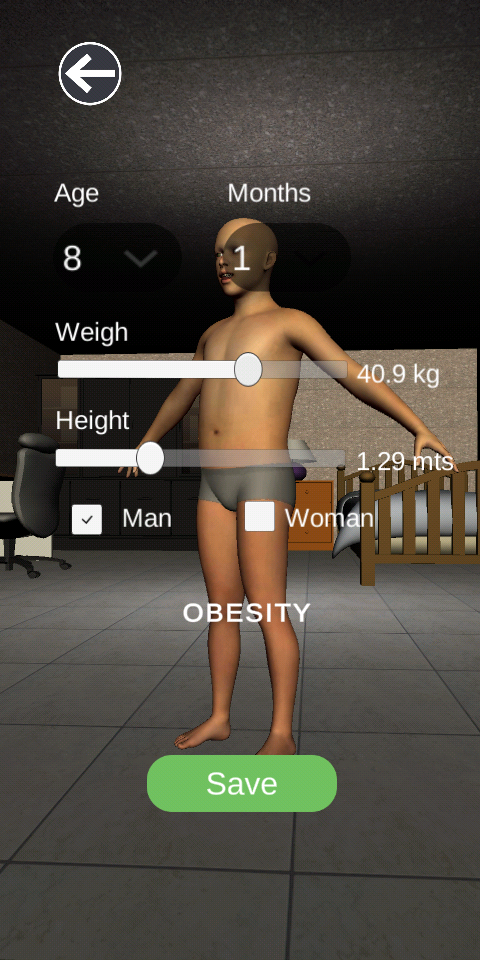
\includegraphics[width=0.25\textwidth]{Figs/Echartea2}&
         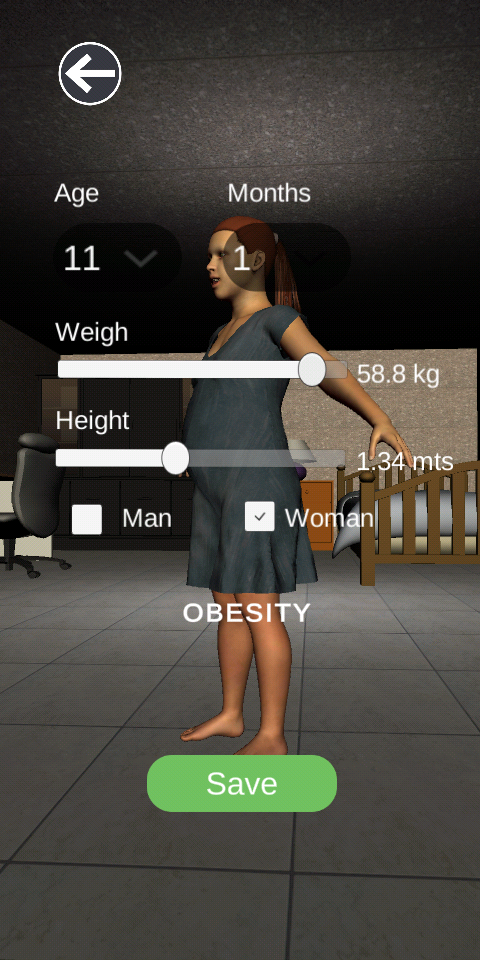
\includegraphics[width=0.25\textwidth]{Figs/Echartea3}\\
          \end{tabular}
\end{center}
%\end{block} 
\end{frame}

%\begin{frame}{Proyectos de Investigación}
\begin{frame}{\citetitle{\EntradaBibtex} (3)}
%\begin{block}{Simulación de modelo de diabetes en un dispositivo móvil (2)} 
\begin{center}
     \begin{tabular}{cc}
         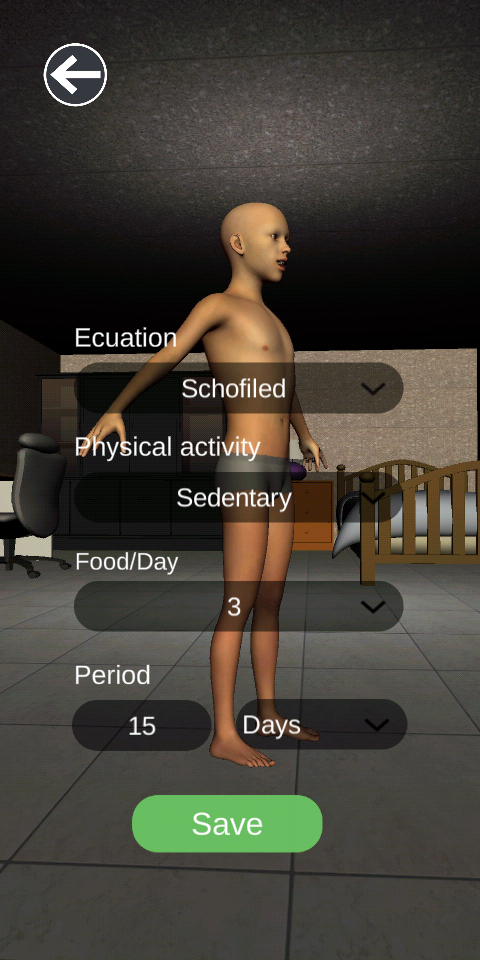
\includegraphics[width=0.25\textwidth]{Figs/Echartea4}&
         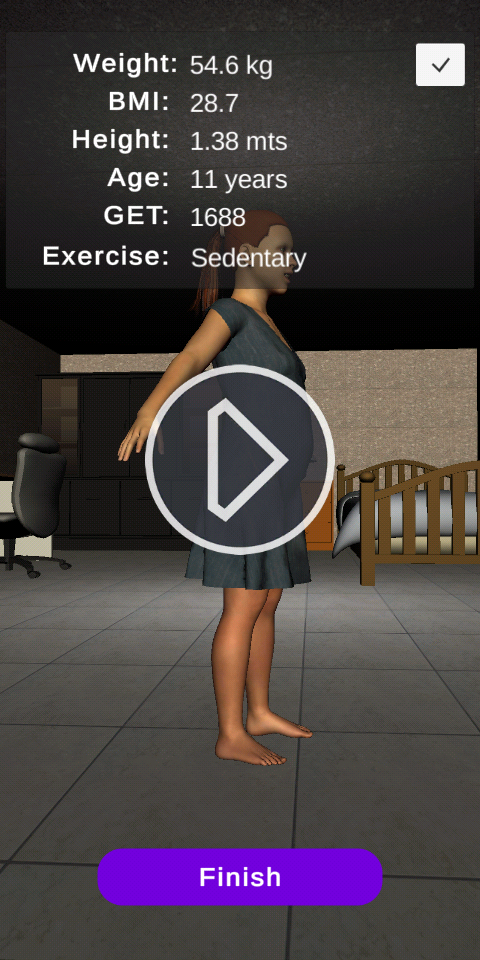
\includegraphics[width=0.25\textwidth]{Figs/Echartea5}
          \end{tabular}
\end{center}
%\end{block} 
\end{frame}


%\renewcommand{\EntradaBibtex}{MarcoNuno_ReporteTecnicoMosaicoOstiones2022_C}


%\begin{frame}{\citetitle{MarcoNuno_ReporteTecnico2022_C} \footnotemark[2] (1)}
%\begin{frame}{\citetitle{MarcoNuno_ReporteTecnico2022_C}$^*$  (1)}
\begin{frame}{\citetitle{\EntradaBibtex} \footnotemark[1] (1)}
%\begin{frame}{---}
%\footfullcite*{MarcoNuno_ReporteTecnico2022_C}

\begin{columns}
\begin{column}{0.70\textwidth}
	\begin{itemize}
		\item Una vez que los ostiones han sido reproducidos, se requiere llevar un registro de su crecimiento mediante conteo. 
        \item Herramientas Software a utilizar: Python (PC), OpenCV, y Android Studio
        \item Herramientas Hardwware a utilizar: Teléfono inteligente (para captura imágenes), adaptador teléfono-microscopio
	\end{itemize}
\end{column}
\begin{column}{0.30\textwidth}  
\begin{center}
     \begin{tabular}{cc}
         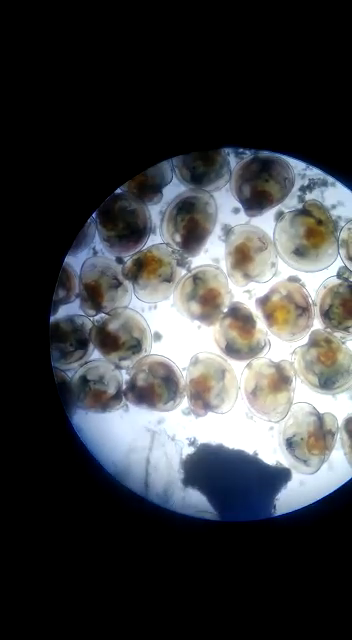
\includegraphics[width=0.68\textwidth]{2022_ConteoOstioncitos/figs/R0063.png}\\         
      \end{tabular}
\end{center}
\end{column} 
\end{columns} 


%\footnotetext[1]{\fullcite{MarcoNuno_ReporteTecnico2022_C}}
%\setcounter{footnote}{0}
%\footnotetext{\fullcite{MarcoNuno_ReporteTecnico2022_C}}
%\footfullcite{MarcoNuno_ReporteTecnico2022_C}
\footnotetext[1]{\fullcite{\EntradaBibtex}}
\end{frame}


%\begin{frame}{\citetitle{MarcoNuno_ReporteTecnico2022_C} (2)}
\begin{frame}{\citetitle{\EntradaBibtex} (2)}
\begin{columns}
\begin{column}{0.38\textwidth}
Problemas Encontrados:
\begin{itemize}
        \item Iluminación variable
        \item Ruido
	\end{itemize}
\textbf{Entrada}: Una secuencia de imágenes continua (video) en donde el técnico manipula la platina para abarcar un número de muestras mayor
\end{column}
\begin{column}{0.64\textwidth}  
\begin{center}
     \begin{tabular}{c}
         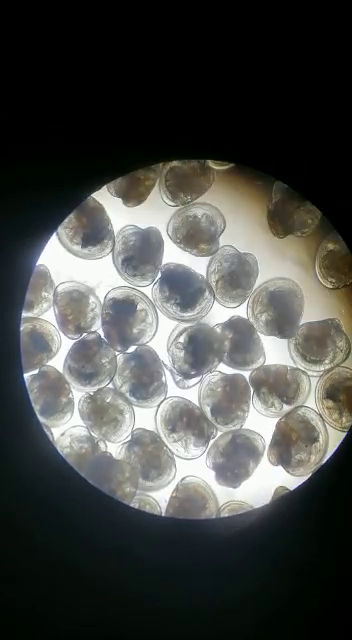
\includegraphics[width=0.24\textwidth]{2022_ConteoOstioncitos/figs/R0078.png}
         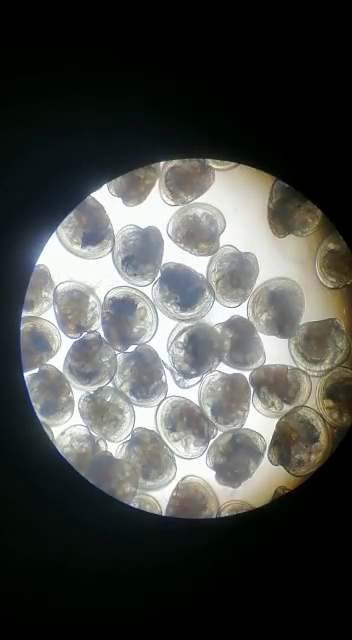
\includegraphics[width=0.24\textwidth]{2022_ConteoOstioncitos/figs/R0090.png}
         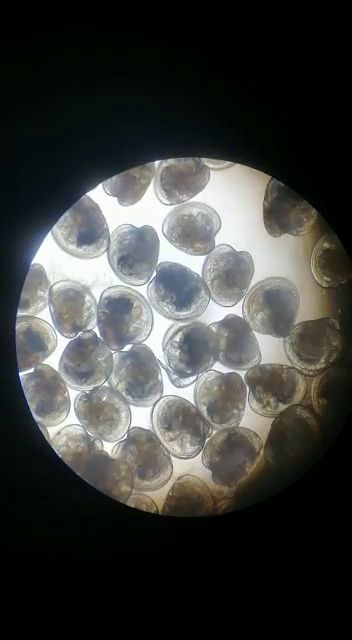
\includegraphics[width=0.24\textwidth]{2022_ConteoOstioncitos/figs/R0102.png}
         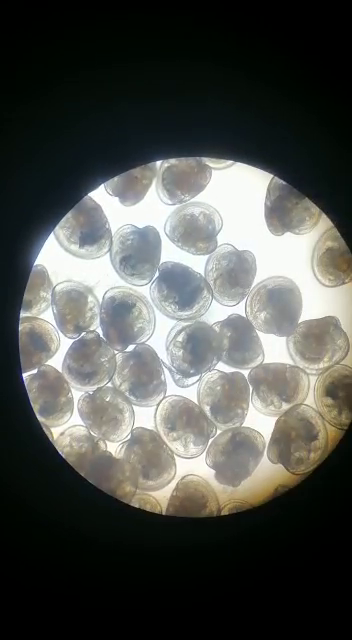
\includegraphics[width=0.24\textwidth]{2022_ConteoOstioncitos/figs/R0126.png}\\
          \end{tabular}
\end{center}
\end{column} 
\end{columns} 
\end{frame}

%\begin{frame}{\citetitle{MarcoNuno_ReporteTecnico2022_C} (3)}
\begin{frame}{\citetitle{\EntradaBibtex} (3)}



Etapas del algoritmo en desarrollo:
\begin{itemize}
        \item Encontrar los puntos característicos y los descriptores de caracteristícas, y estimar una correspondencia
        \item A partir de la correspondencia, estimar la matriz de Homografía y llevar a cabo transformación de tipo Warp para estimar el empalme de imágenes
	\end{itemize}

\begin{center}
 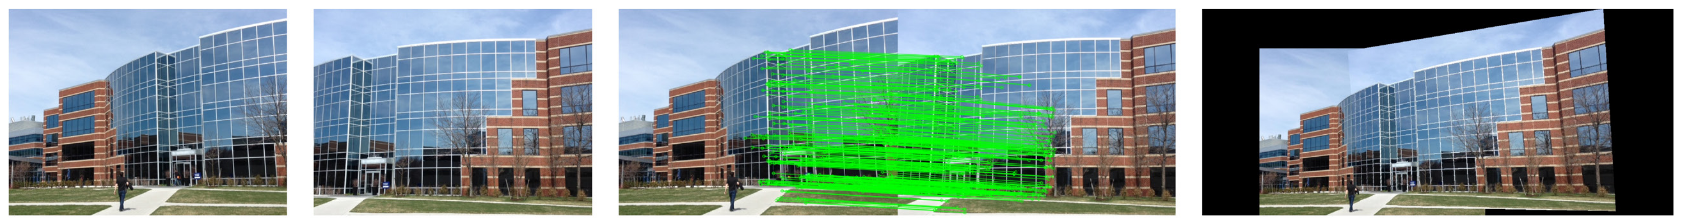
\includegraphics[width=0.95\textwidth]{2022_ConteoOstioncitos/figs/ImageMatchingAndRegistration.png}
\end{center}

\end{frame}


%\begin{frame}{\citetitle{MarcoNuno_ReporteTecnico2022_C} (4)}
\begin{frame}{\citetitle{\EntradaBibtex} (4)}
\begin{center}
 \begin{tabular}{c}
         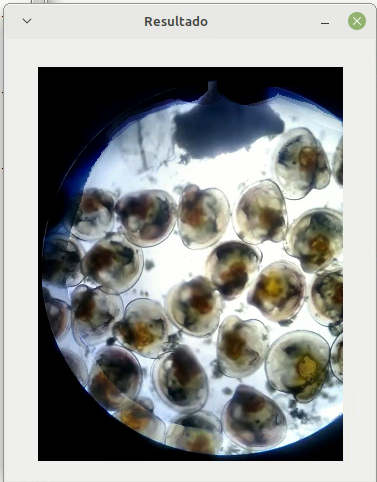
\includegraphics[width=0.24\textwidth]{2022_ConteoOstioncitos/figs/0049.png}
         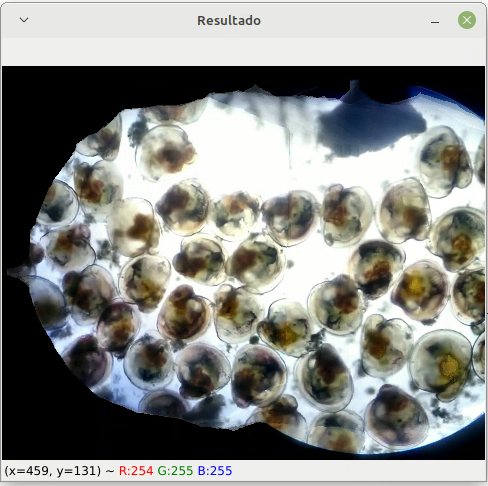
\includegraphics[width=0.24\textwidth]{2022_ConteoOstioncitos/figs/0085.png}
         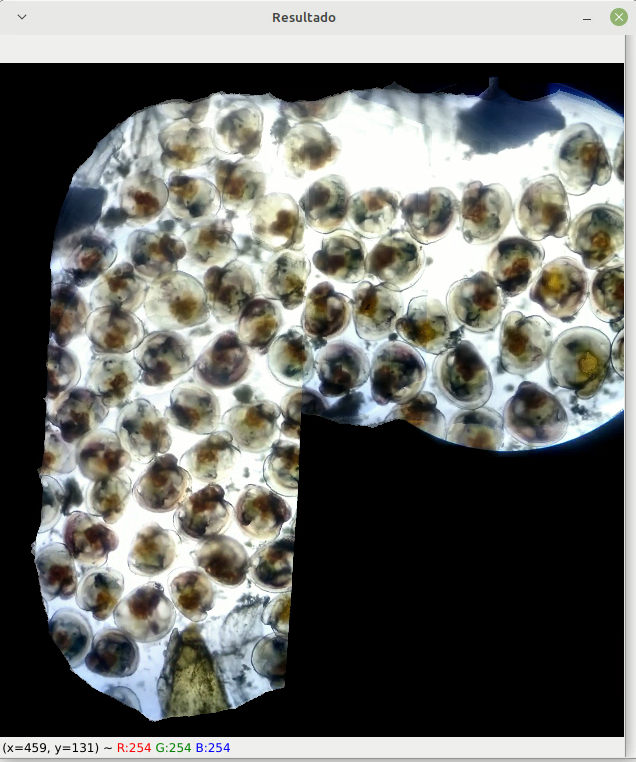
\includegraphics[width=0.24\textwidth]{2022_ConteoOstioncitos/figs/0193.png}
         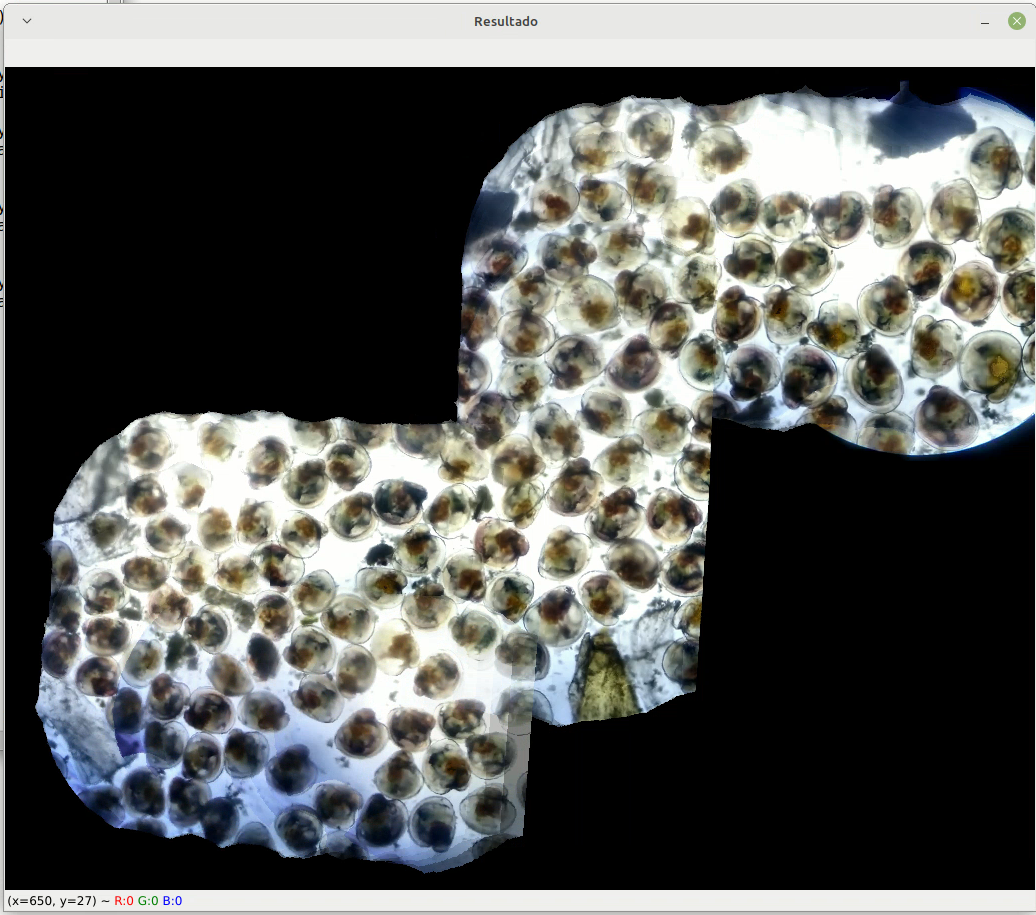
\includegraphics[width=0.24\textwidth]{2022_ConteoOstioncitos/figs/0373.png}\\
          \end{tabular}
\end{center}
\end{frame}



%\begin{frame}{\citetitle{MarcoNuno_ReporteTecnico2022_C} (5)}
\begin{frame}{\citetitle{\EntradaBibtex} (5)}
Resultado final de la generación del mosaico y del conteo de ostiones
\begin{center}
 \begin{tabular}{c}
         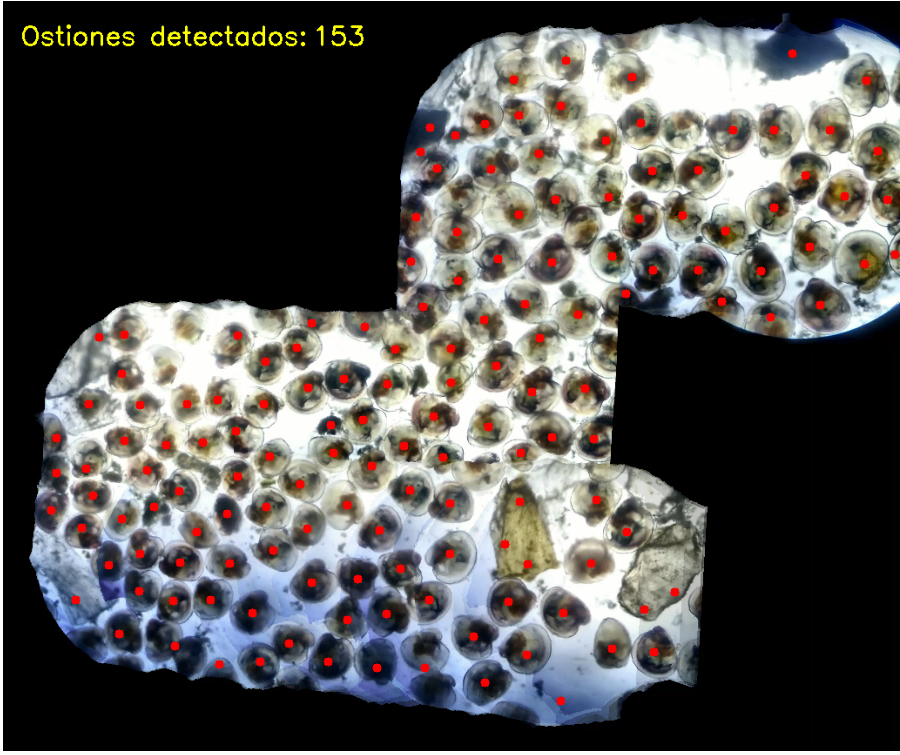
\includegraphics[width=0.50\textwidth]{2022_ConteoOstioncitos/figs/ConteoOstionesFinal.png}\\
          \end{tabular}
\end{center}

\end{frame}



\begin{frame}{\citetitle{MarcoNuno_ReporteTecnico2022_C} (6)}

\begin{itemize}
\item Hay un avance significativo con respecto al prototipo versión PC (cerca de completarse)
\begin{itemize} 
\item Se requieren más imágenes, que incluyan el conteo realizado de manera manual para contrastarlo con nuestros algoritmos
\item Posiblemente se deban afinar los algoritmos que se tienen desarrollados
\end{itemize}
\item Con respecto a la fase en el teléfono inteligente, se lleva un avance del 10\%, a reserva de la incorporación de un estudiante de estancia o estadía
\item Los resultados apuntan que es posible publicar los resultados en una Revista Indexada por el JCR
\end{itemize}




\end{frame}




%\renewcommand{\EntradaBibtex}{MarcoNuno_ReporteTecnicoMicroAlgas2022}

%\begin{frame}{\citetitle{MarcoNuno_ReporteTecnico2022}  \footnotemark{} (1)}
%\begin{frame}{\citetitle{MarcoNuno_ReporteTecnico2022}  \footnote{\fullcite{MarcoNuno_ReporteTecnico2022}} (1)}
\begin{frame}{\citetitle{\EntradaBibtex} \footnotemark[1] (1)}
%\begin{frame}{}
%\footfullcite*{MarcoNuno_ReporteTecnico2022}
\begin{columns}
\begin{column}{0.6\textwidth}
	\begin{itemize}  %del cuerpo académico Acuicultura Sustentable (UTMTB-CA-1)
        \item Proyecto desarrollado  en colaboración con investigadores de la Universidad Tecnológica del Mar de Tamaulipas Bicentenario (UTMarT)
		\item Desarrollar una herramienta para automatizar el conteo de microalgas, específicamente de las especies \textit{Isochrysis galbana} e \textit{Chaetoceros muelleri}
        \item Herramientas Software a utilizar: Python (PC), OpenCV, y Android Studio
        \item Herramientas Hardwware a utilizar: Teléfono inteligente (para captura imágenes), adaptador teléfono-microscopio
	\end{itemize}
\end{column}
\begin{column}{0.4\textwidth}  
\begin{center}
     \begin{tabular}{cc}
         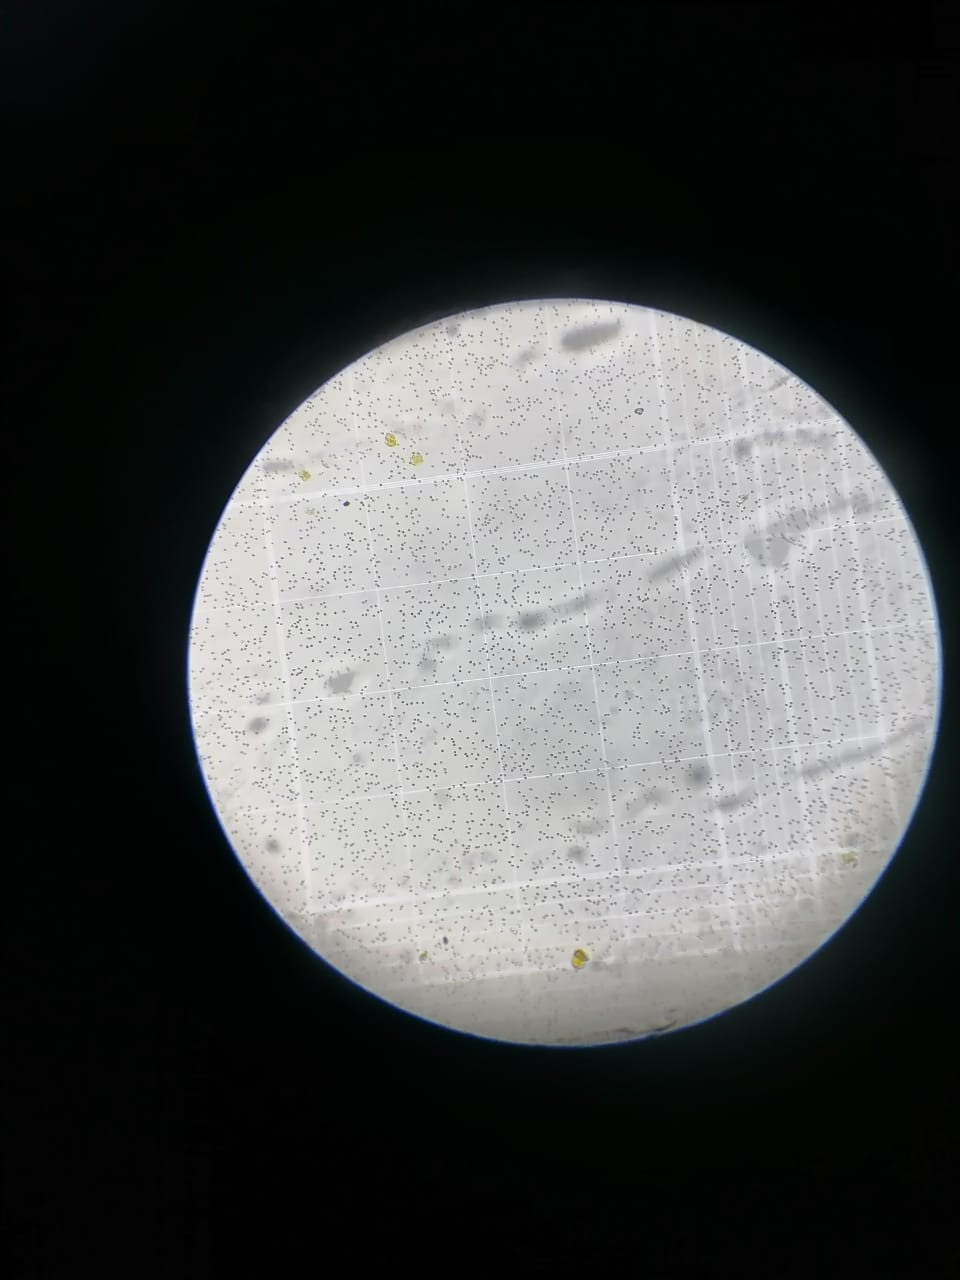
\includegraphics[width=0.68\textwidth]{2022_ConteoMicroAlgas/figs/MicroAlgas01}\\         
      \end{tabular}
\end{center}
\end{column} 
\end{columns} 


%\footnotetext[1]{\fullcite{MarcoNuno_ReporteTecnico2022}}
%\setcounter{footnote}{0}
%\footnotetext{\fullcite{MarcoNuno_ReporteTecnico2022}}
%\footfullcite{MarcoNuno_ReporteTecnico2022}
\footnotetext[1]{\fullcite{\EntradaBibtex}}
\end{frame}


\begin{frame}{\citetitle{\EntradaBibtex} (2)}
\begin{columns}
\begin{column}{0.6\textwidth}
Problemas Encontrados:
\begin{itemize}
        \item Rotación de la rejilla de referencia
        \item Nivel de acercamiento es variable
		\item Imágenes con ruido, distancia de captura variable, regionres con desenfoque 
        \item Problemas de contraste (complica encontrar las lineas)
        \item Cuando hay muchas algas, hay grupos de algas que suelen formar lineas falsas
	\end{itemize}
\end{column}
\begin{column}{0.4\textwidth}  
\begin{center}
     \begin{tabular}{cc}
         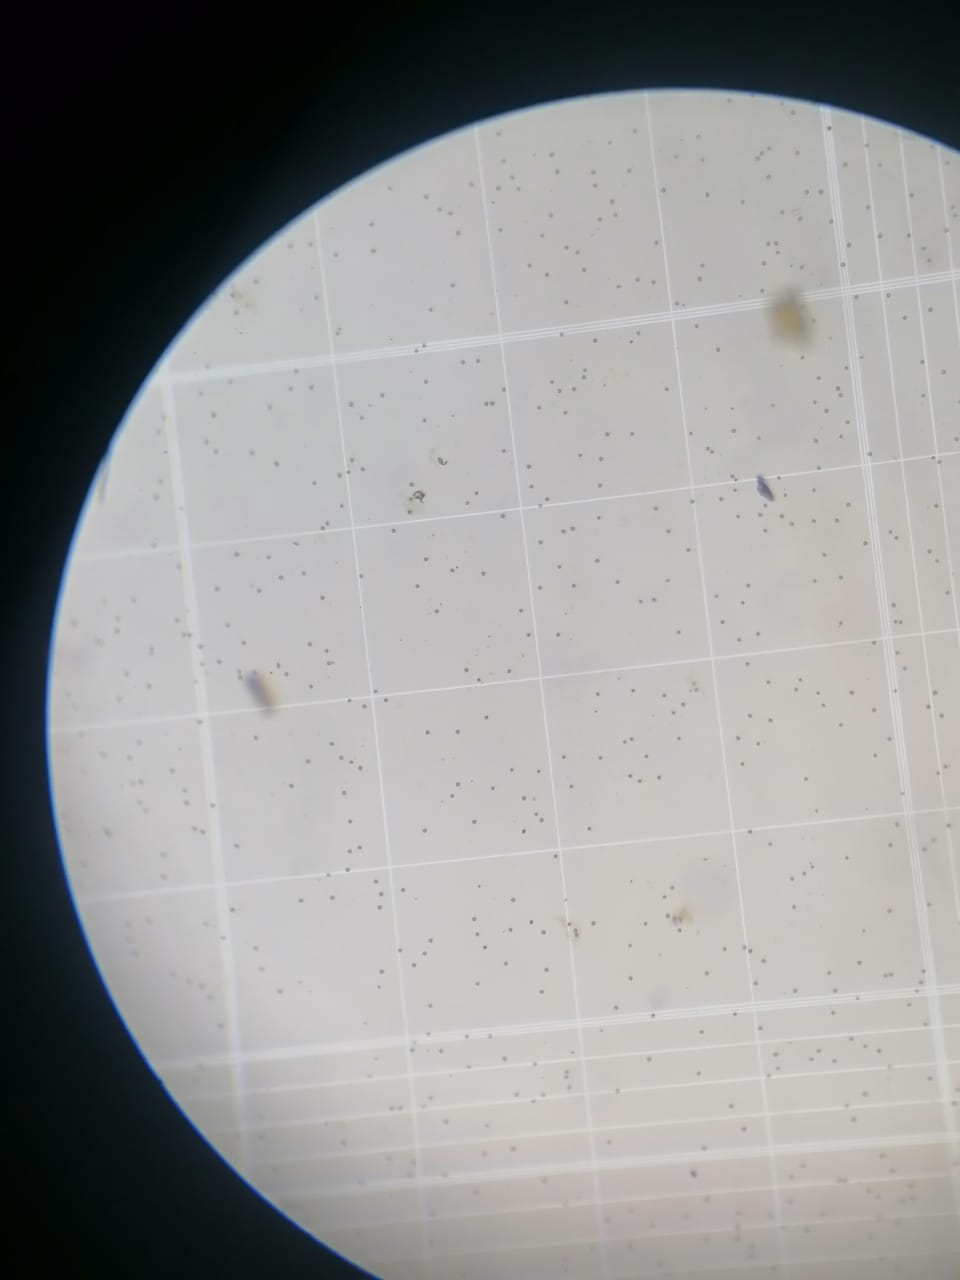
\includegraphics[width=0.38\textwidth]{2022_ConteoMicroAlgas/figs/CuadranteA}&
         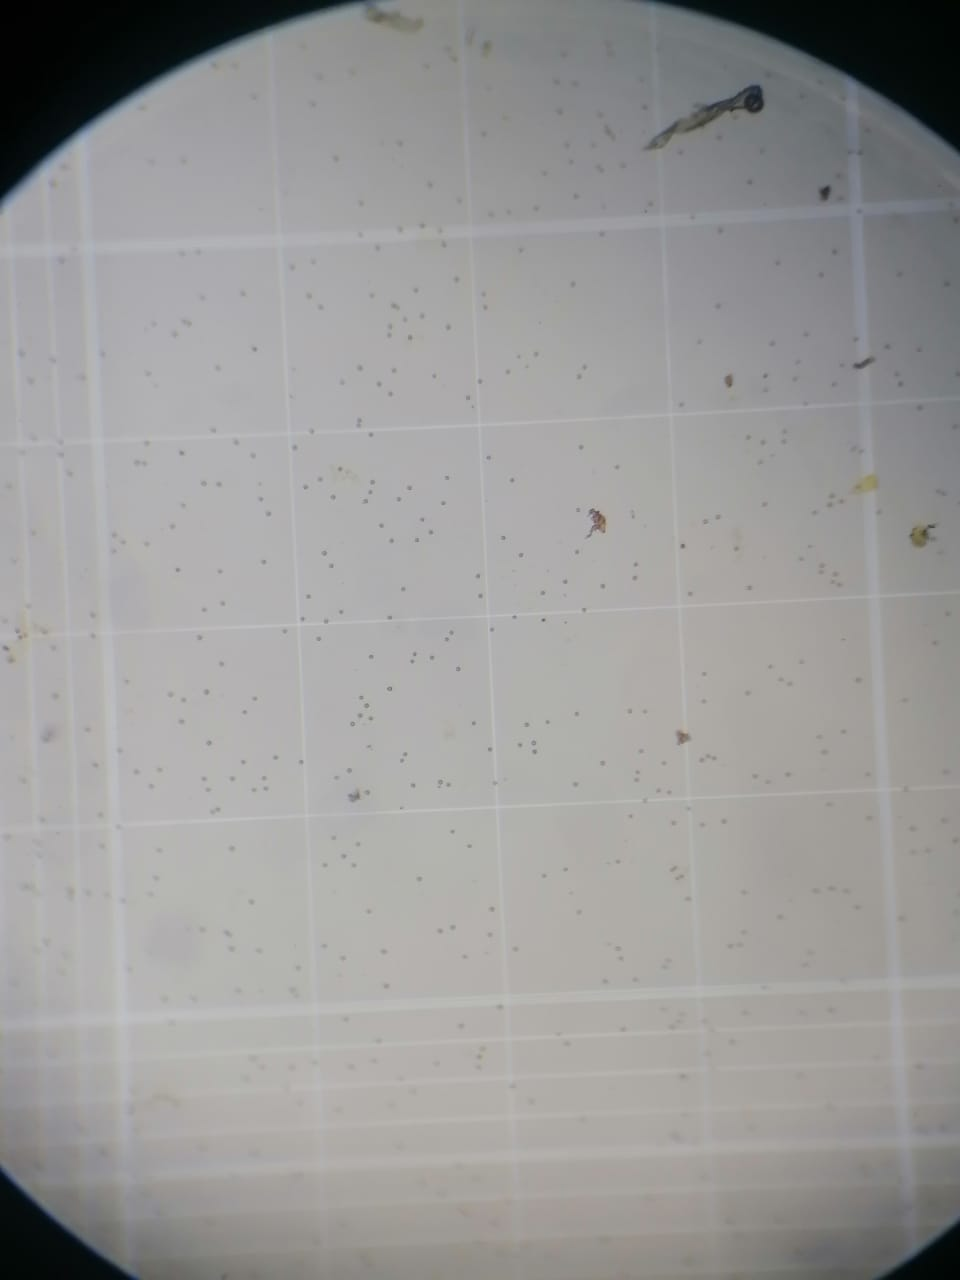
\includegraphics[width=0.38\textwidth]{2022_ConteoMicroAlgas/figs/CuadranteB}\\
         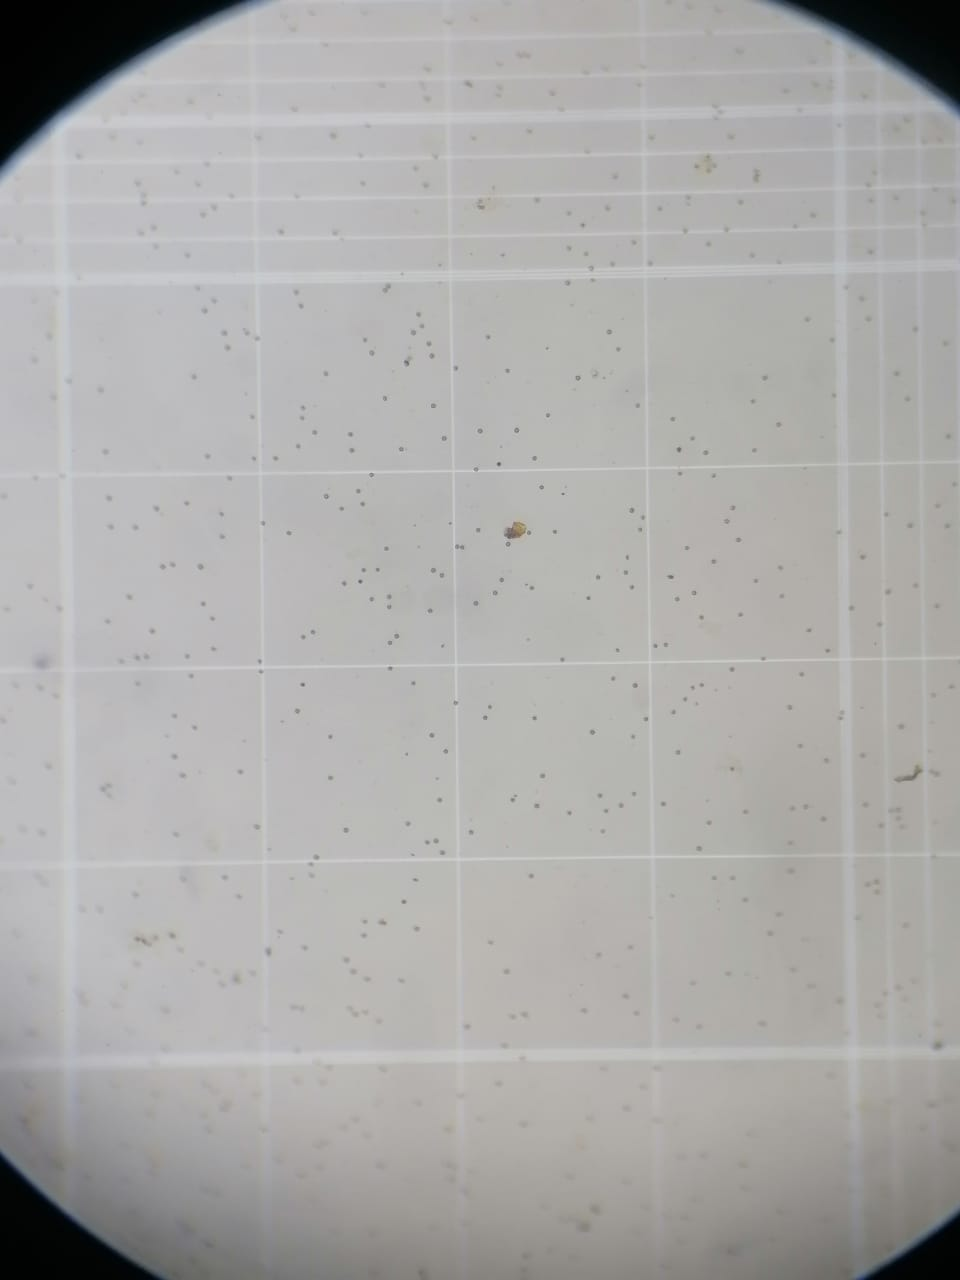
\includegraphics[width=0.38\textwidth]{2022_ConteoMicroAlgas/figs/CuadranteC}&
         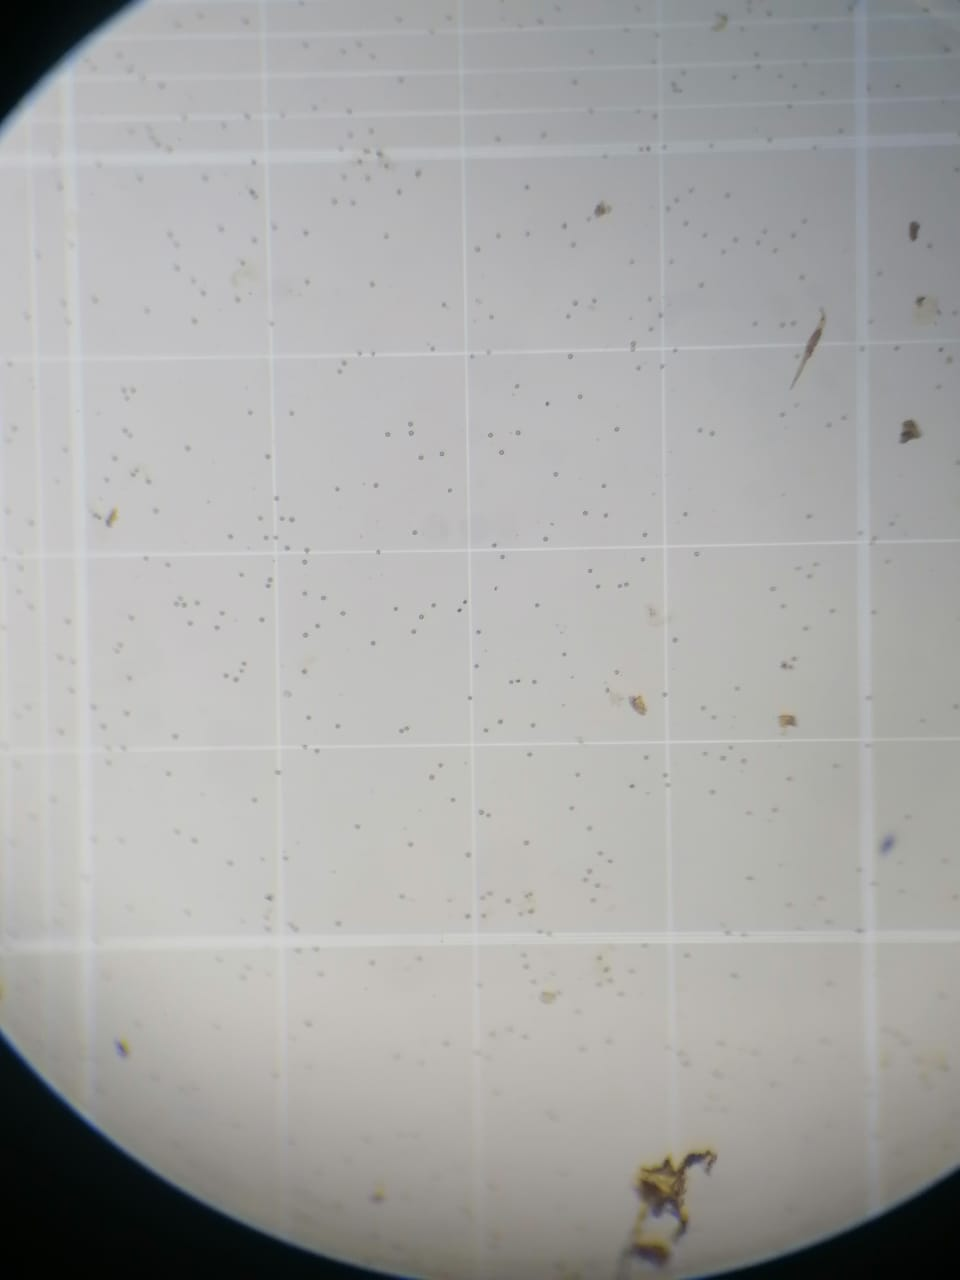
\includegraphics[width=0.38\textwidth]{2022_ConteoMicroAlgas/figs/CuadranteD}\\
          \end{tabular}
\end{center}
\end{column} 
\end{columns} 
\end{frame}


\begin{frame}{\citetitle{\EntradaBibtex} (3)}
\begin{columns}
\begin{column}{0.50\textwidth}
Fases del algoritmo en desarrollo:
\begin{itemize}
		\item Binalizar las imágenes y aplicar un algoritmo de detección de bordes
        \item Encontrar las líneas mediante los algoritmos de Hough Standard y Probabilístico
        \item Analizar las líneas encontradas para determinar aquellas que deben descartarse 
        \item Efectuar un enmascarado de regiones para aislar solo la rejilla delimitadora
        \item Llevar a cabo el conteo de las algas a partir de los contornos de la imágen de bordes
	\end{itemize}
\end{column}
\begin{column}{0.50\textwidth}  
\begin{center}
     \begin{tabular}{ccc}
         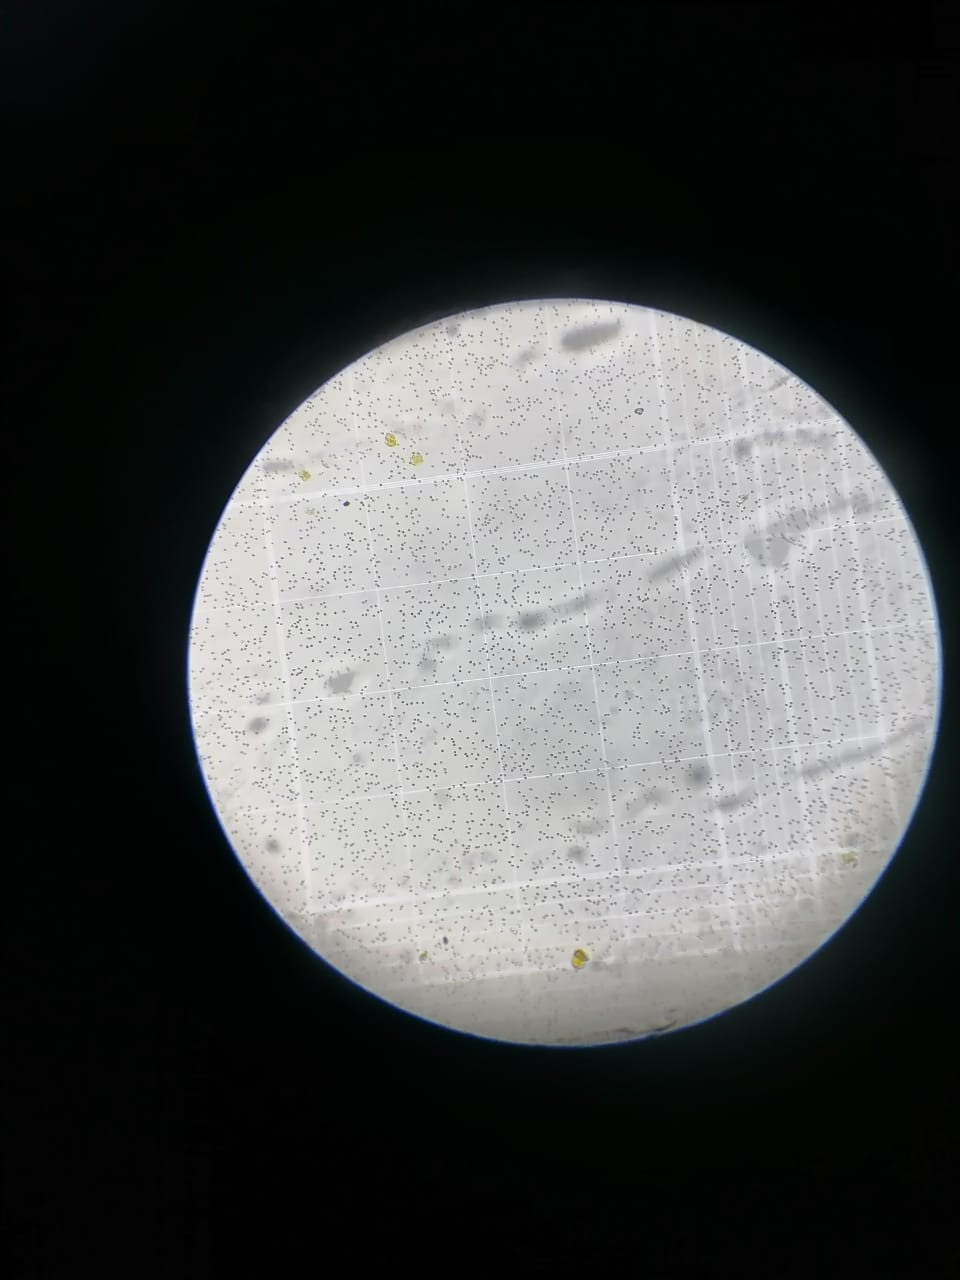
\includegraphics[width=0.31\textwidth]{2022_ConteoMicroAlgas/figs/MicroAlgas01}&
         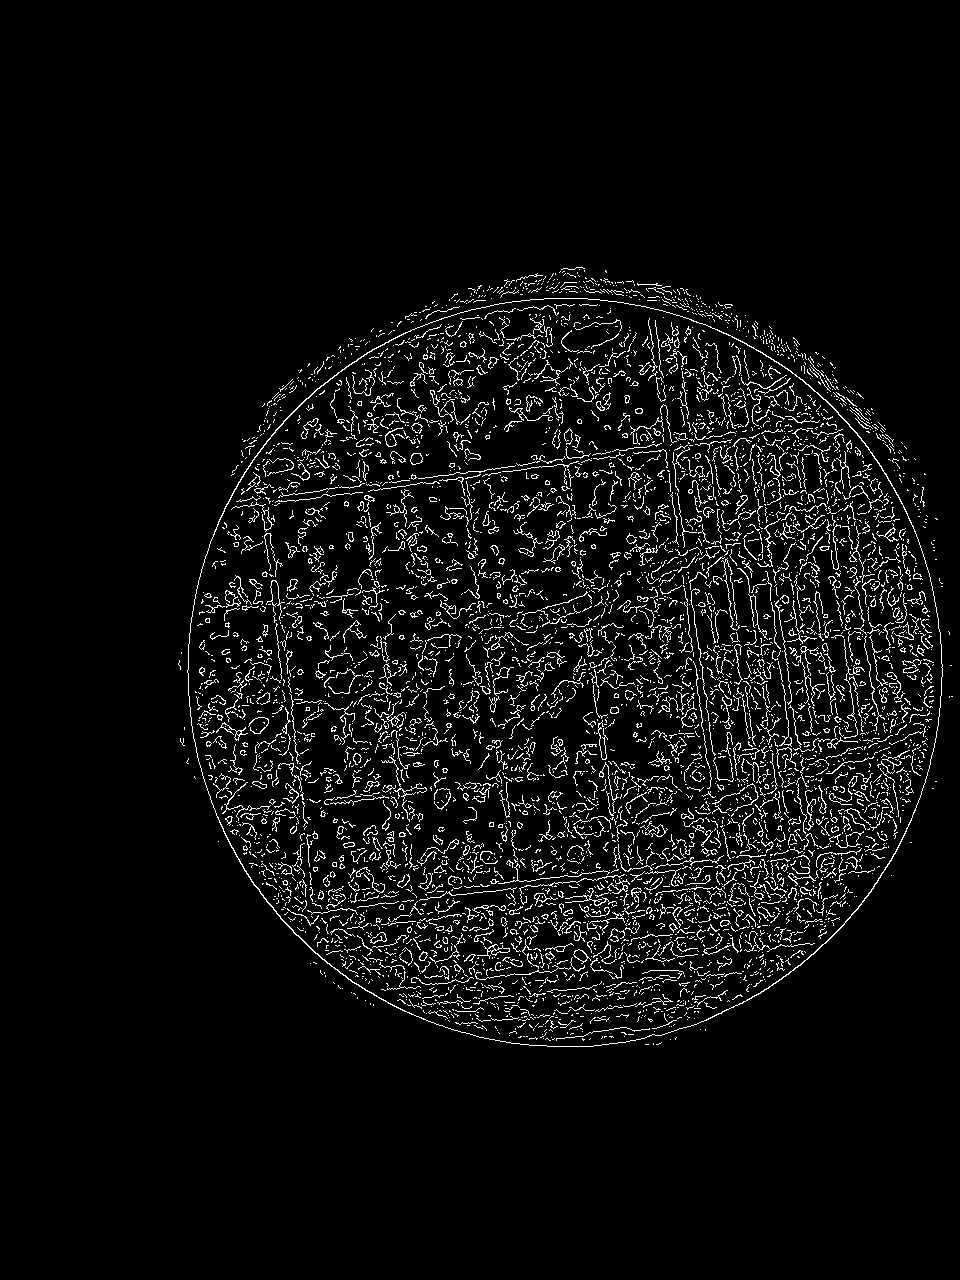
\includegraphics[width=0.31\textwidth]{2022_ConteoMicroAlgas/figs/02_Canny}&
         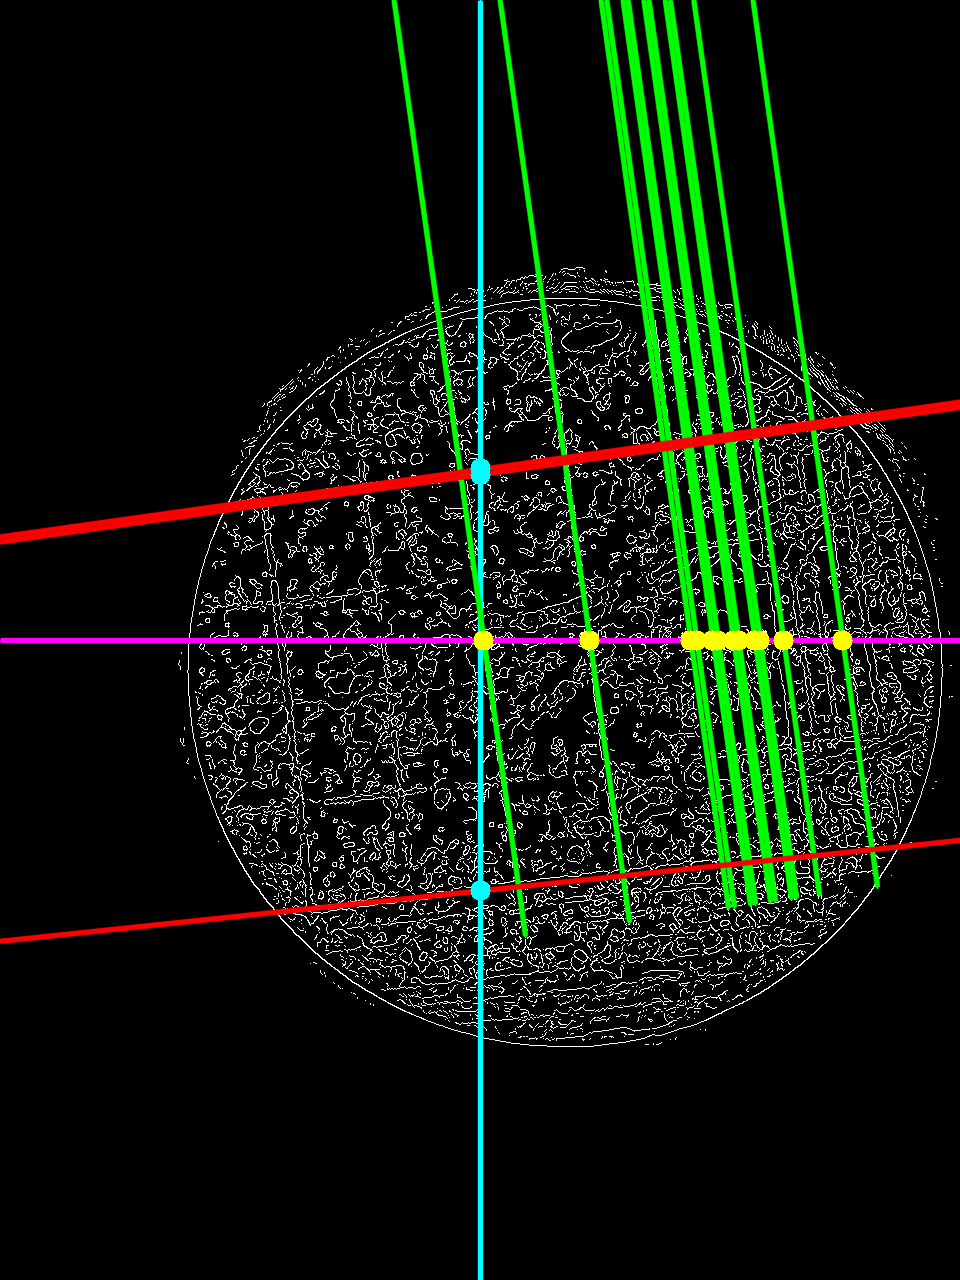
\includegraphics[width=0.31\textwidth]{2022_ConteoMicroAlgas/figs/03_LineasEstandar}\\
         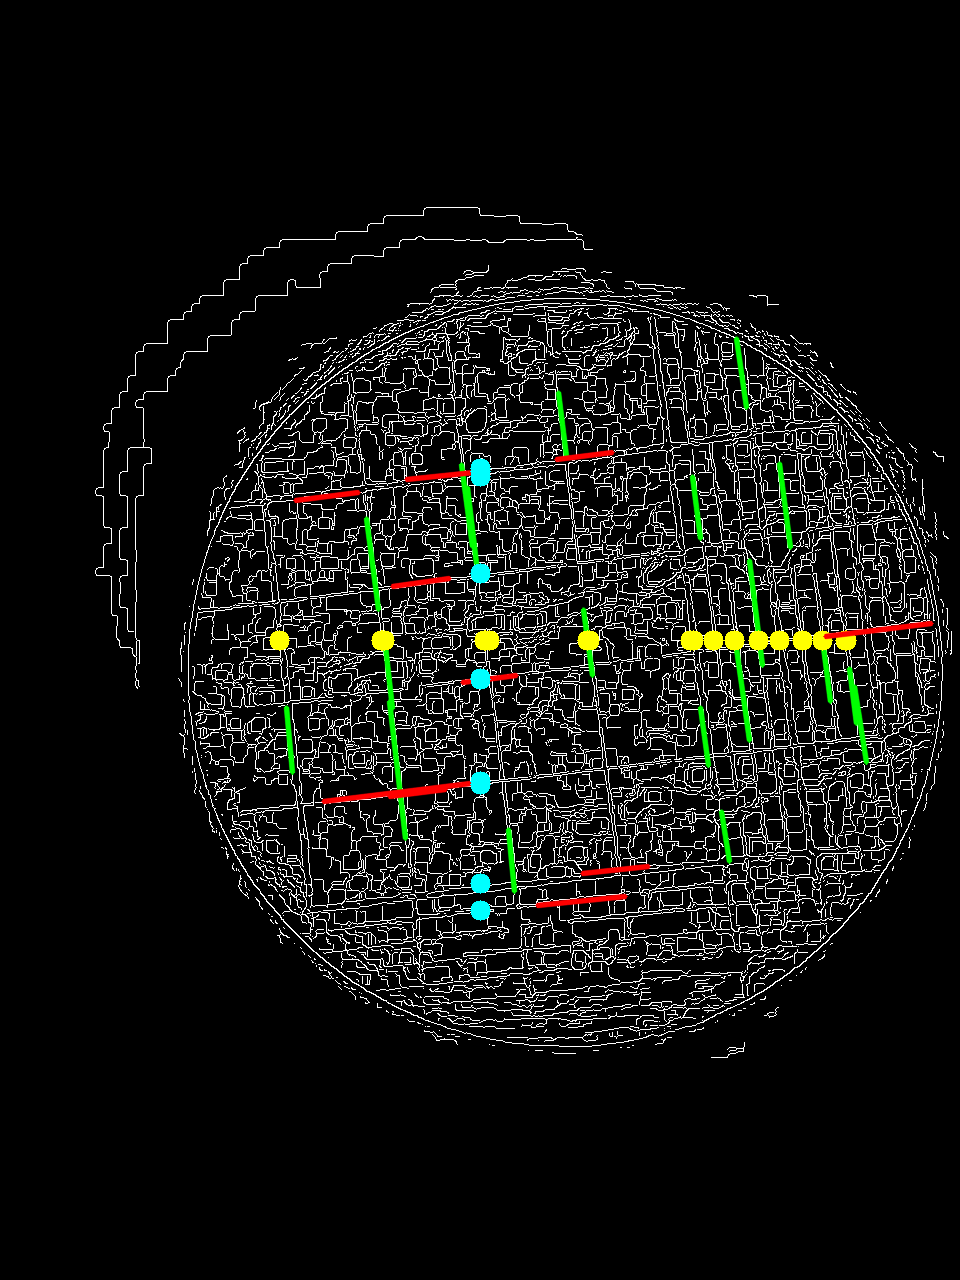
\includegraphics[width=0.31\textwidth]{2022_ConteoMicroAlgas/figs/04_LineasProbabilistico}&
         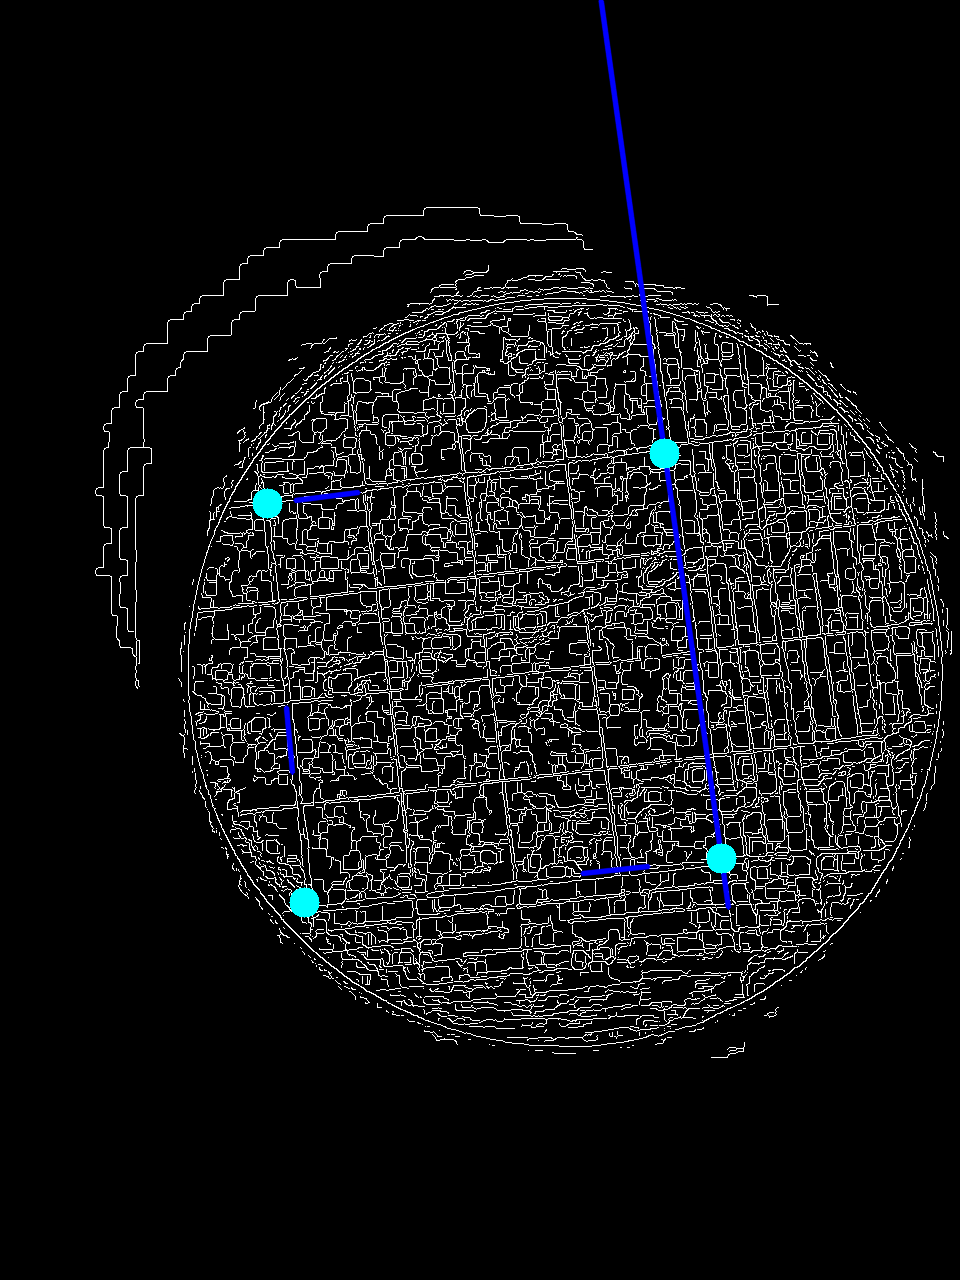
\includegraphics[width=0.31\textwidth]{2022_ConteoMicroAlgas/figs/05_Delimitacion}&
         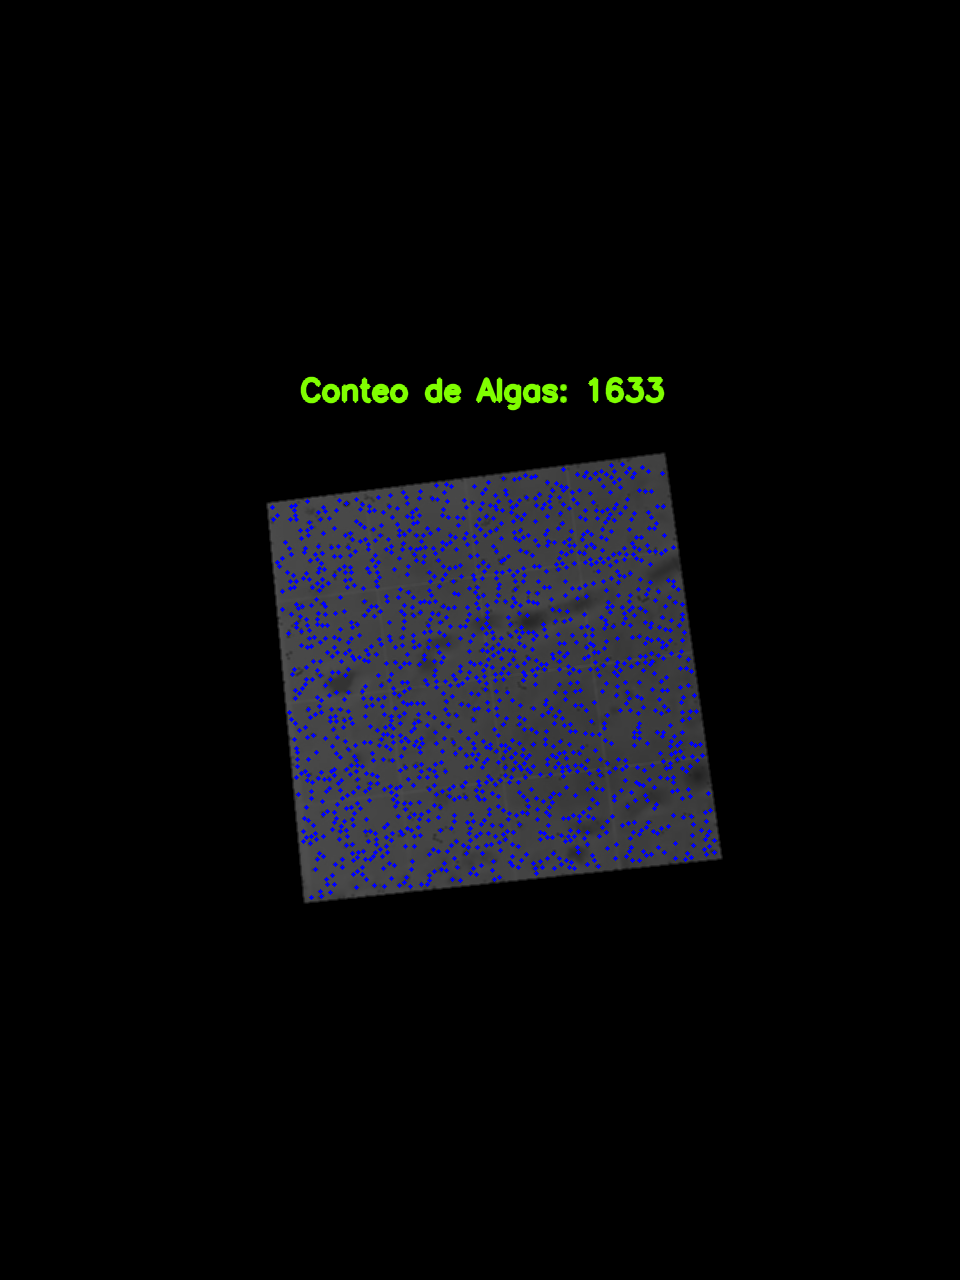
\includegraphics[width=0.31\textwidth]{2022_ConteoMicroAlgas/figs/07_ResultadoConteo}\\

          \end{tabular}
\end{center}
\end{column} 
\end{columns} 
\end{frame}



\begin{frame}{\citetitle{\EntradaBibtex} (4)}

\begin{itemize}
\item Hay un avance significativo con respecto al prototipo versión PC (cerca de completarse)
\begin{itemize} 
\item Se requieren más imágenes, que incluyan el conteo realizado de manera manual para contrastarlo con nuestros algoritmos
\item Posiblemente se deban afinar los algoritmos que se tienen desarrollados
\end{itemize}
\item Con respecto a la fase en el teléfono inteligente, se lleva un avance del 20\%, a reserva de la incorporación de un estudiante de estancia o estadía
\item Los resultados apuntan que es posible publicar los resultados en una Revista Indexada por el JCR
\end{itemize}
\end{frame}





%\renewcommand{\EntradaBibtex}{MarcoNuno_Revista_2022_03_00}

\begin{frame}{\citetitle{\EntradaBibtex} \footnotemark[1] (1)}
\begin{columns}
\begin{column}{0.6\textwidth}
	\begin{itemize}
		\item Una solución al problema de manejo de desechos es el reciclado
        \item Específicamente, la separación por color de una botella es de utilidad para su correcto manejo
        \item Se propone un sistema para clasificar botellas en una banda transportadora
        \item El nucleo del sistema es una arquictectura hardware que realiza tareas de visión para clasificación tiempo real 
	\end{itemize}
\end{column}
\begin{column}{0.4\textwidth}  
\begin{center}
     \begin{tabular}{cc}
         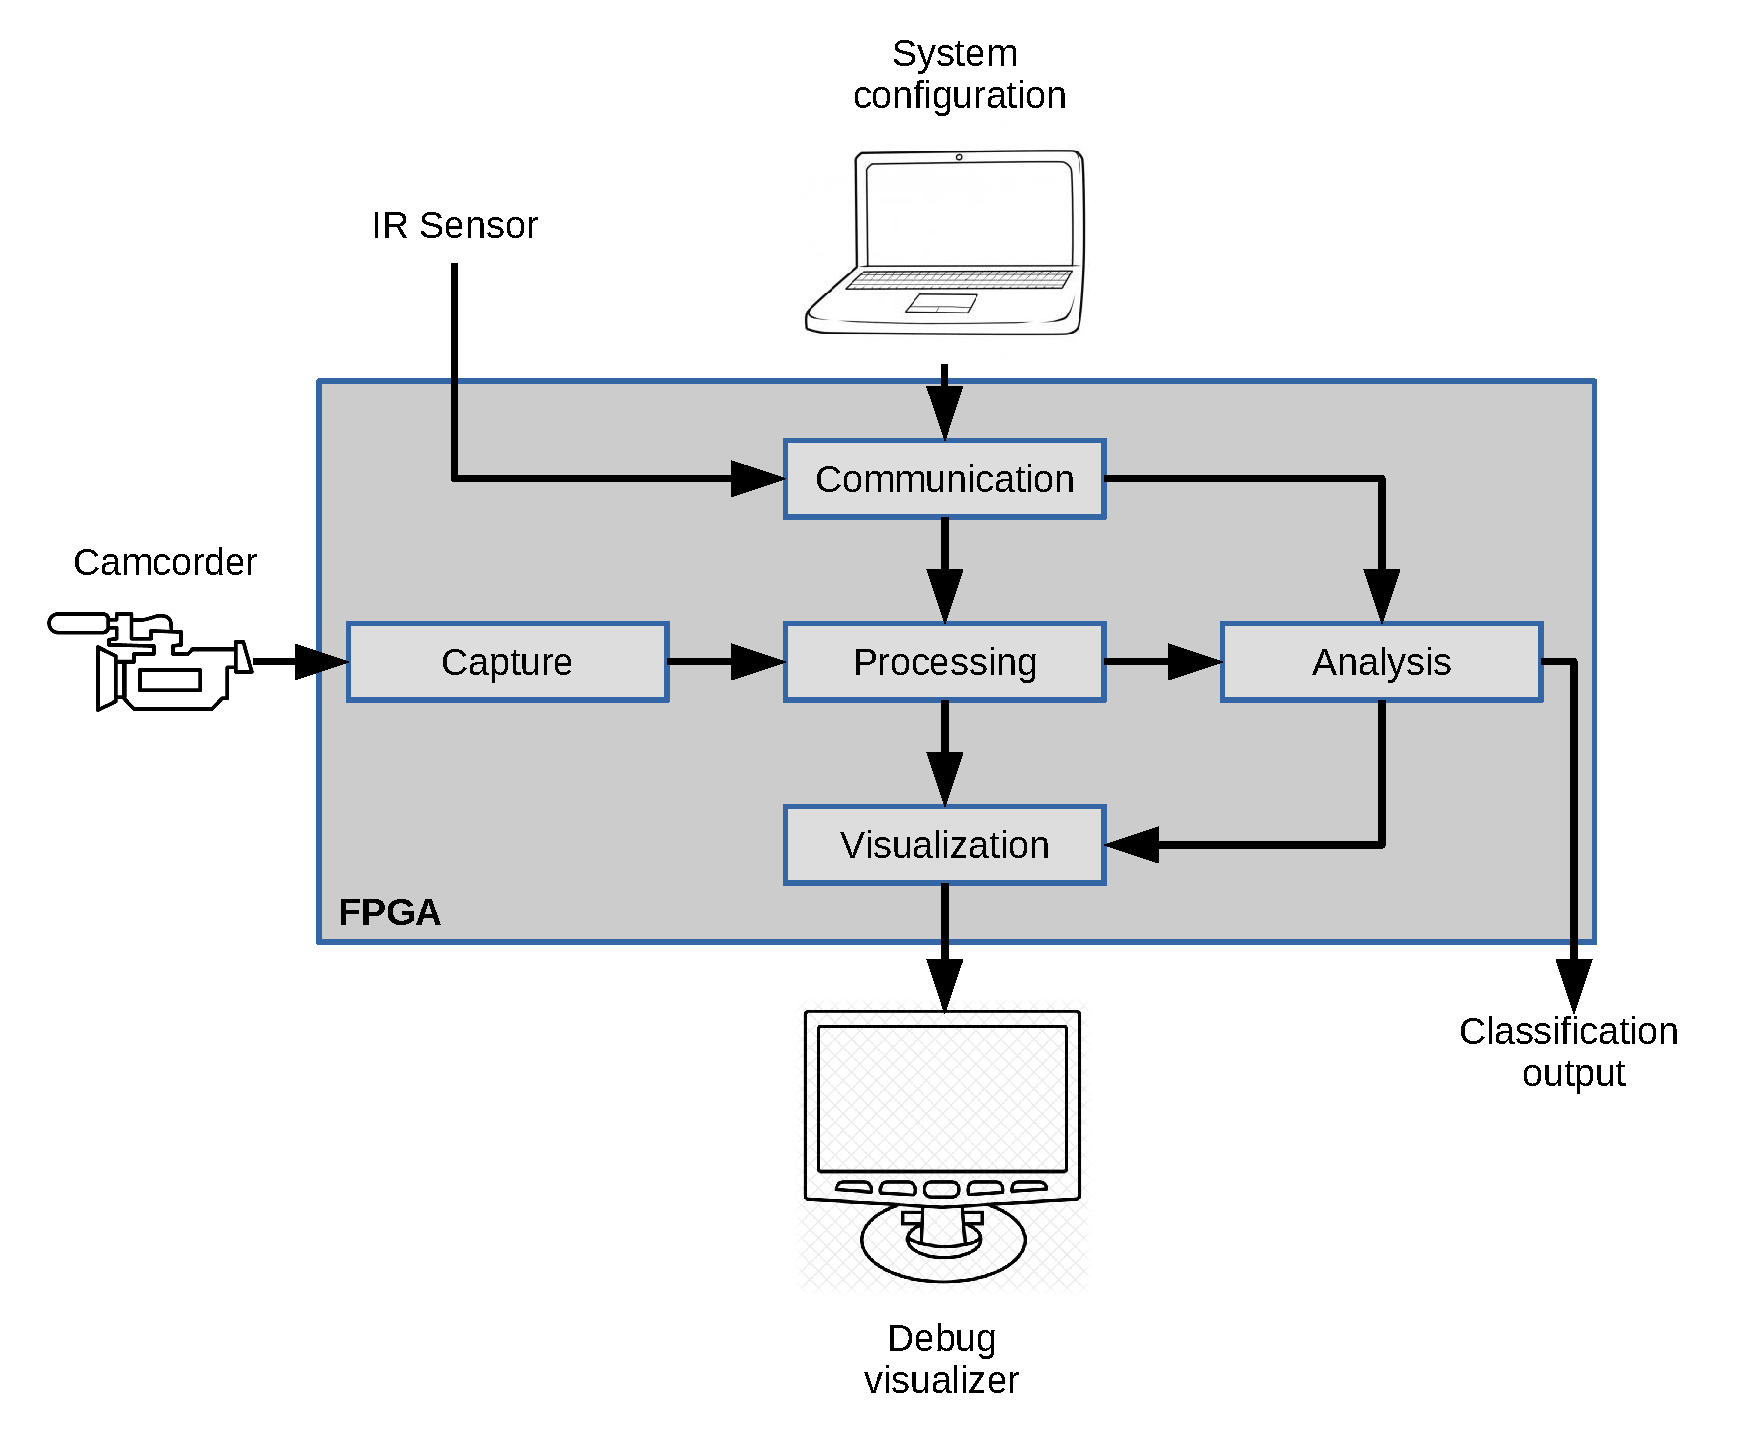
\includegraphics[width=0.98\textwidth]{2022_BottleClassifier/figs/MainModules.pdf}\\         
      \end{tabular}
\end{center}
\end{column} 
\end{columns} 
\footnotetext[1]{\fullcite{\EntradaBibtex}}
\end{frame}


\begin{frame}{\citetitle{\EntradaBibtex} (2)}
\begin{columns}
\begin{column}{0.5\textwidth}

Materiales:
\begin{itemize}
        \item Sensor óptico de presencia
        \item Tarjeta FPGA - Spartan 6 Industrial Video Processing Kit
        \item Cámara con salida HDMI
        \item Monitor para depuración
        \item Circuitos para activar actuadores de separación de botellas
	\end{itemize}
\end{column}
\begin{column}{0.5\textwidth}  
\begin{center}
     \begin{tabular}{c}
         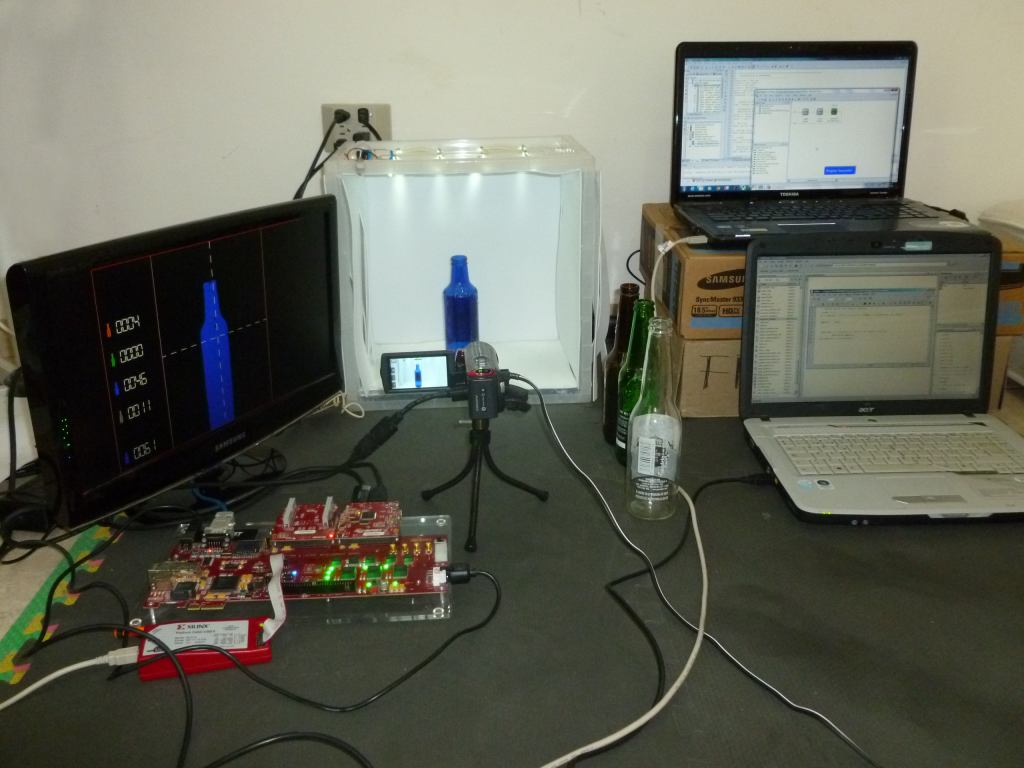
\includegraphics[width=0.98\textwidth]{2022_BottleClassifier/figs/cap4_setup.png}\\
          \end{tabular}
\end{center}
\end{column} 
\end{columns} 
\end{frame}

\begin{frame}{\citetitle{\EntradaBibtex} (3)}
El nucleo del sistema propuesto es el módulo del sistema de visión, que ejecuta las siguientes tareas:
\begin{itemize}
        \item Aplicar filtros (promediado y de mediana)
        \item Convertir de Color a HSV
        \item Efectuar operaciones morfológica
        \item Calcular histograma
        \item En base a reglas previamente definidas, clasifica la botella por color
	\end{itemize}

%\begin{center}
% 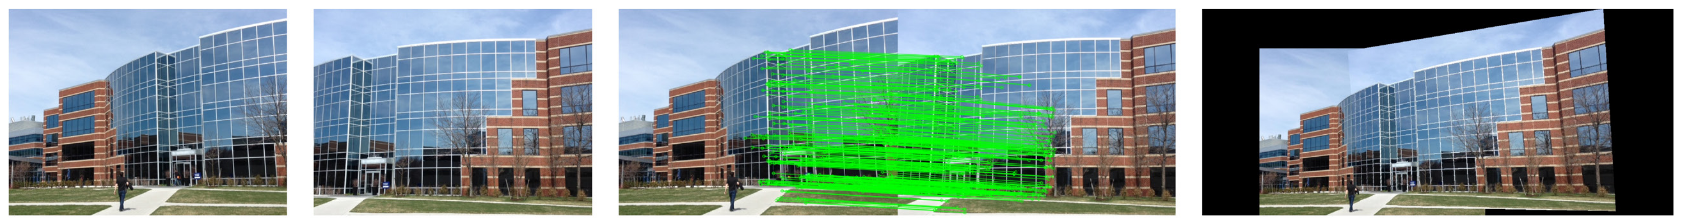
\includegraphics[width=0.95\textwidth]{2022_ConteoOstioncitos/figs/ImageMatchingAndRegistration.png}
%\end{center}

\end{frame}


\begin{frame}{\citetitle{\EntradaBibtex} (4)}
\begin{columns}
\begin{column}{0.6\textwidth}
\begin{itemize}
\item Una vez que el sensor óptico detecta la botella, inicia el procesamiento de imágen
\item Cuando el procesamiento de imágen termina, arroja como resultado la clasificación de la botella
\item Se incrementa un contador de cada botella y se muestra en la pantalla de depuración
\item Es posible configurar los umbrales, para separar botellas de diferente color diferentes
\end{itemize}
\end{column} 
\begin{column}{0.3\textwidth}
 \begin{tabular}{c}
    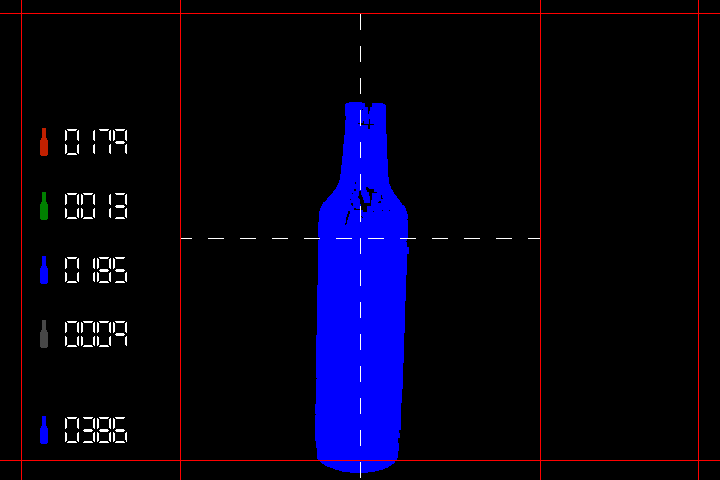
\includegraphics[width=0.98\textwidth]{2022_BottleClassifier/figs/cap4_dispfinal.png}\\
    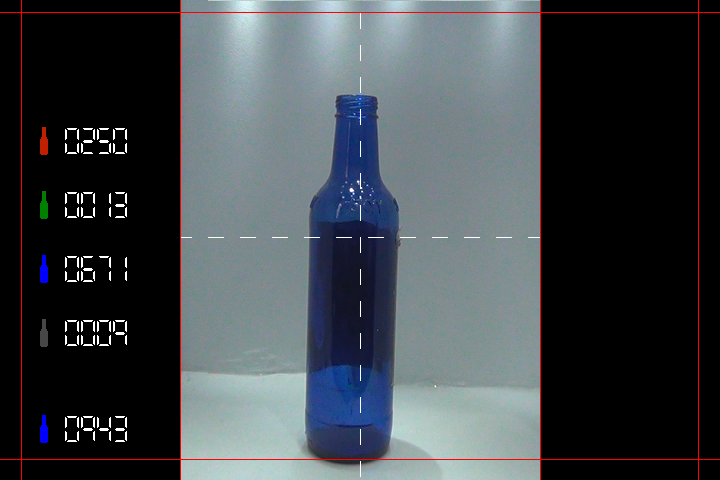
\includegraphics[width=0.98\textwidth]{2022_BottleClassifier/figs/cap4_disporiginal.png}
  \end{tabular}
\end{column} 
\end{columns} 

\end{frame}





%

\renewcommand{\EntradaBibtex}{ProyectoLSM_2022}

\begin{frame}{\citetitle{\EntradaBibtex} \footnotemark[1] (1)}
\begin{columns}
\begin{column}{0.6\textwidth}
	\begin{itemize}
		\item Se propone una aplicación móvil que reconozca el lenguaje de señas mexicano (LSM)
        \item El equipo capturó videos de los diferentes gestos a clasificar (palabras comunes y letras del alfabeto)
        \item Se utilizó la libreria MediaPipe para la obtención de los marcadores de manos, torso y cabeza
        \item Se entrenó una Red Neuronal Convolucional
	\end{itemize}
\end{column}
\begin{column}{0.4\textwidth}  
\begin{center}
     \begin{tabular}{cc}

         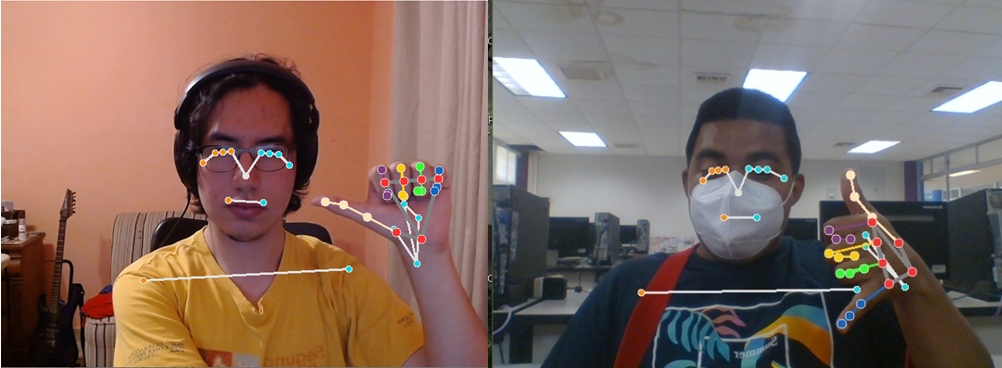
\includegraphics[width=0.98\textwidth]{2022_AplicacionLSM/figs/Diapositiva1.PNG}\\         
      \end{tabular}
\end{center}
\end{column} 
\end{columns} 
\footnotetext[1]{\fullcite{\EntradaBibtex}}
\end{frame}


\begin{frame}{\citetitle{\EntradaBibtex} (2)}
\begin{columns}
\begin{column}{0.6\textwidth}
Librerías utilizadas:
\begin{itemize}
        \item Tensorflow (PC) y Tensorflow-lite (Smartphone)
		\item MediPipe
	\end{itemize}
Para cada video:
\begin{itemize}
        \item Se normaliza la duración del video a una duración estándard
		\item Se entraen ubicaciones de los marcadores y se estiman angulos
		\item Se anexa al dataset para su posterior entrenamiento
	\end{itemize}
\end{column}
\begin{column}{0.4\textwidth}  
\begin{center}
     \begin{tabular}{c}
         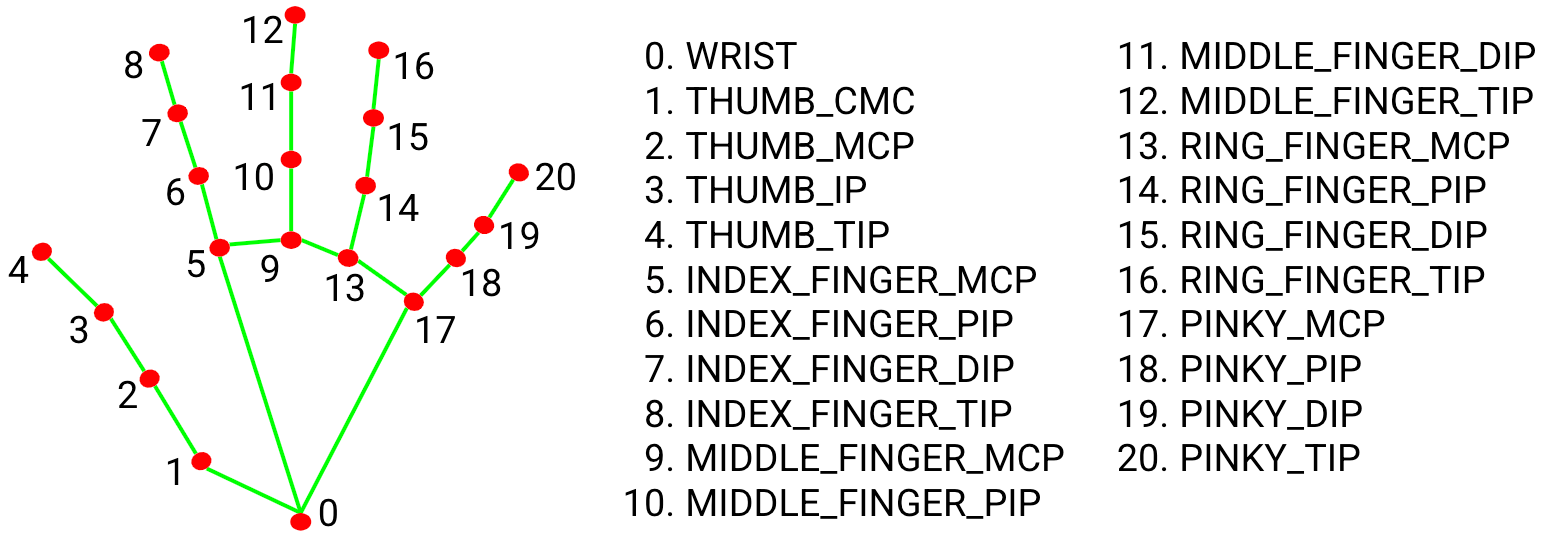
\includegraphics[width=0.98\textwidth]{2022_AplicacionLSM/figs/hand_landmarks.png}\\
          \end{tabular}
\end{center}
\end{column} 
\end{columns} 
\end{frame}

\begin{frame}{\citetitle{\EntradaBibtex} (3)}
Una vez entrenada la red, el modelo se incorpora a la aplicación
\begin{center}
 \begin{tabular}{cccc}
    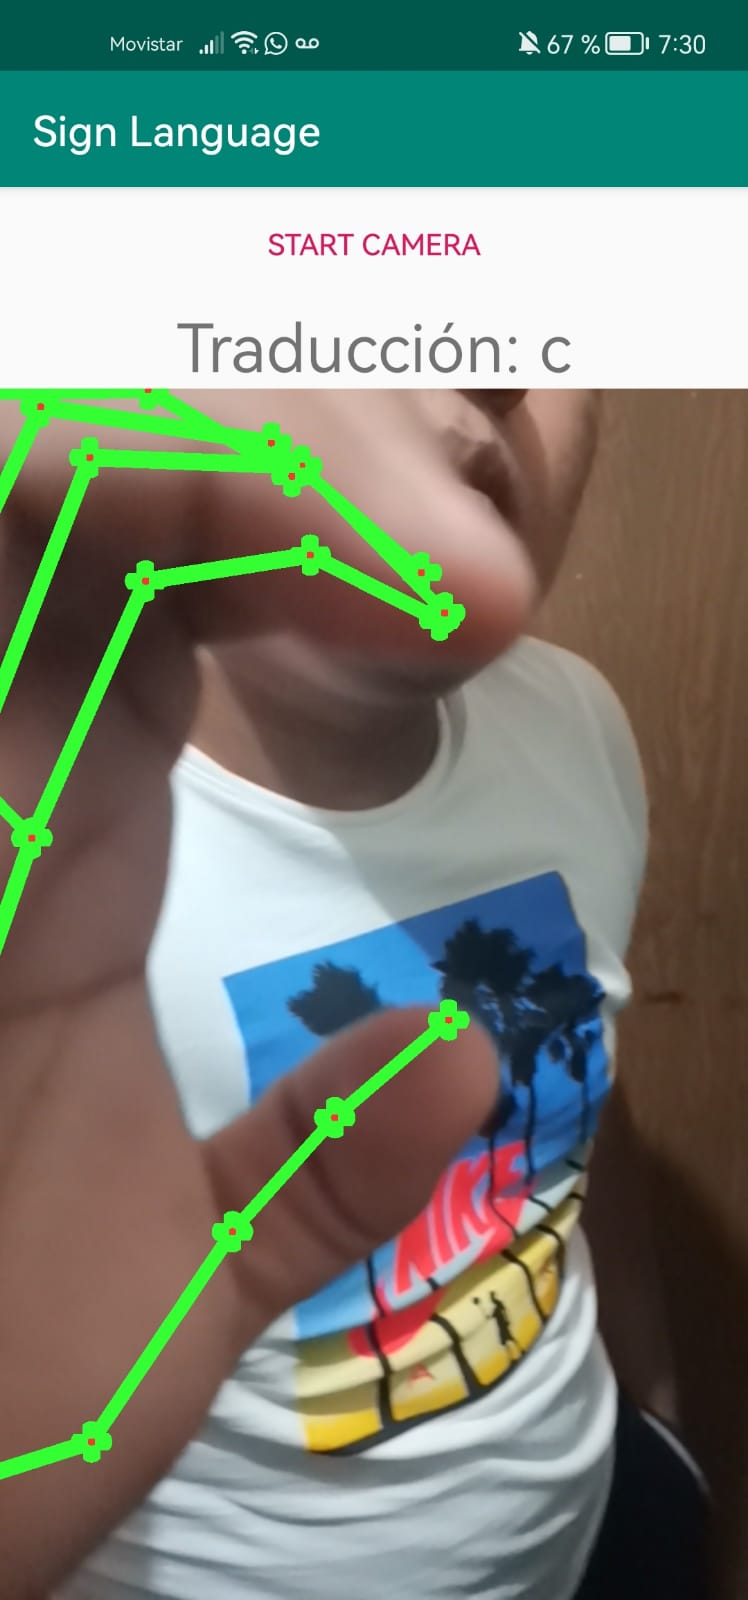
\includegraphics[width=0.16\textwidth]{2022_AplicacionLSM/figs/App1.jpeg}
    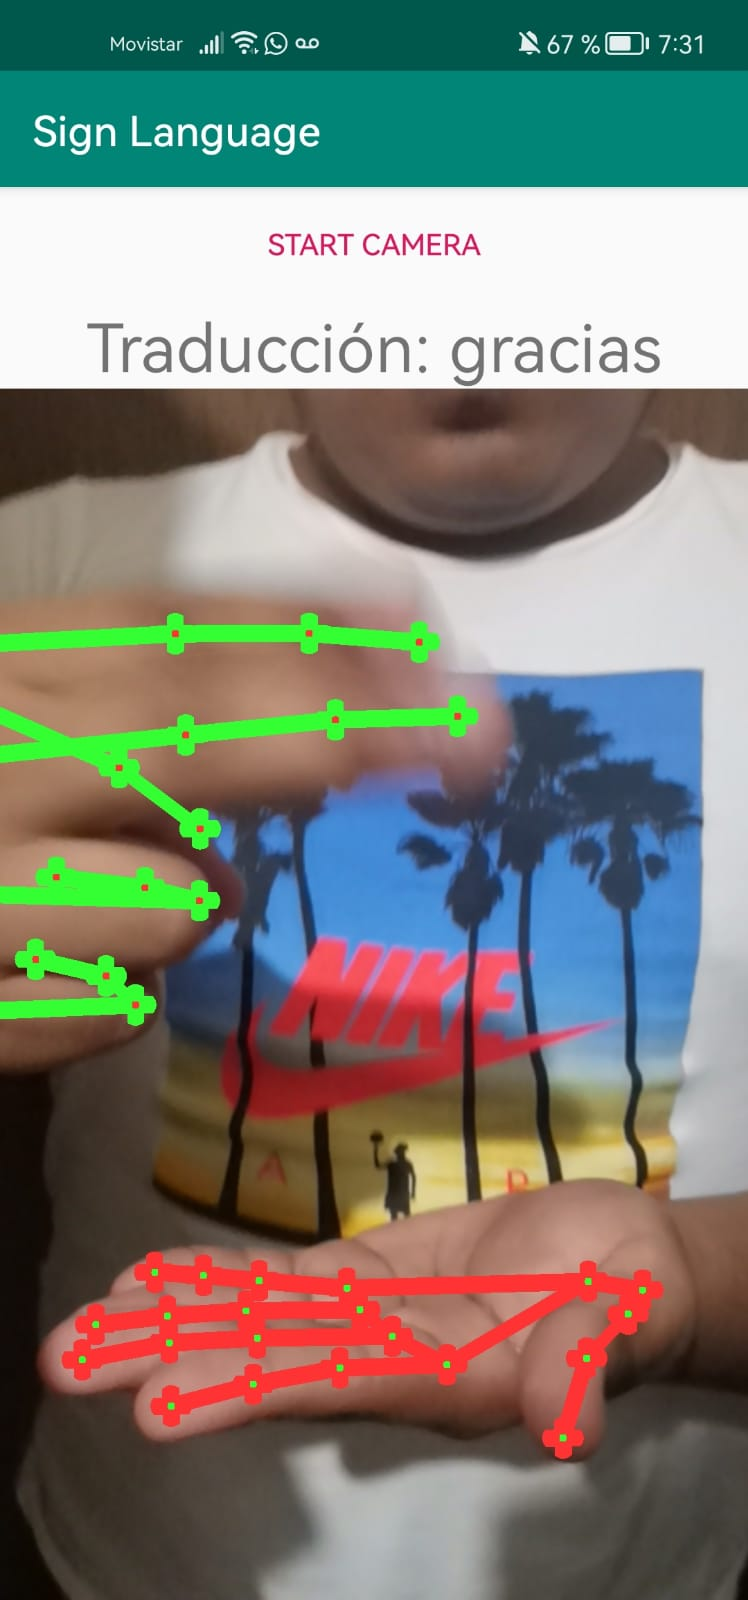
\includegraphics[width=0.16\textwidth]{2022_AplicacionLSM/figs/App2.jpeg}
    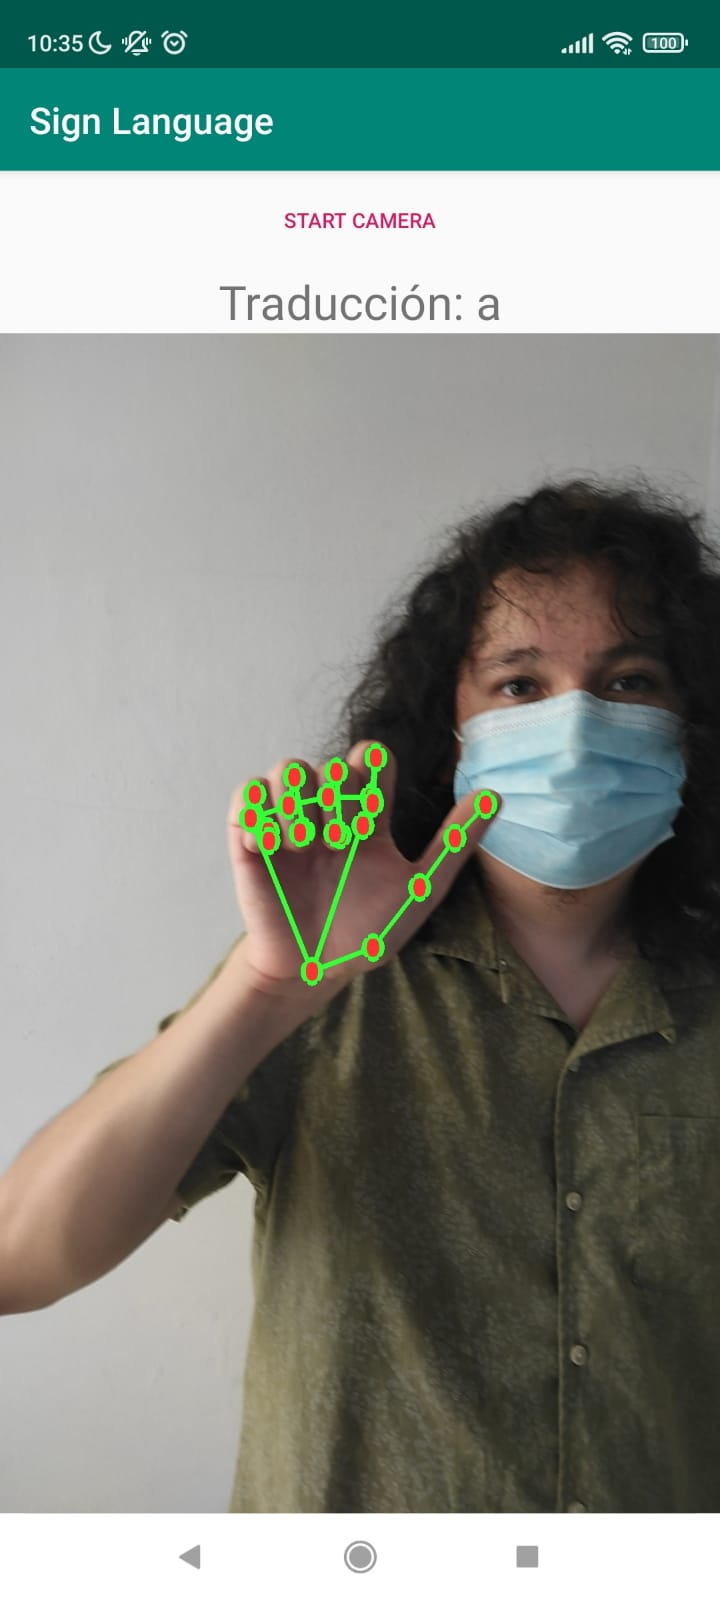
\includegraphics[width=0.16\textwidth]{2022_AplicacionLSM/figs/Muestra_compañeros1.jpeg}
    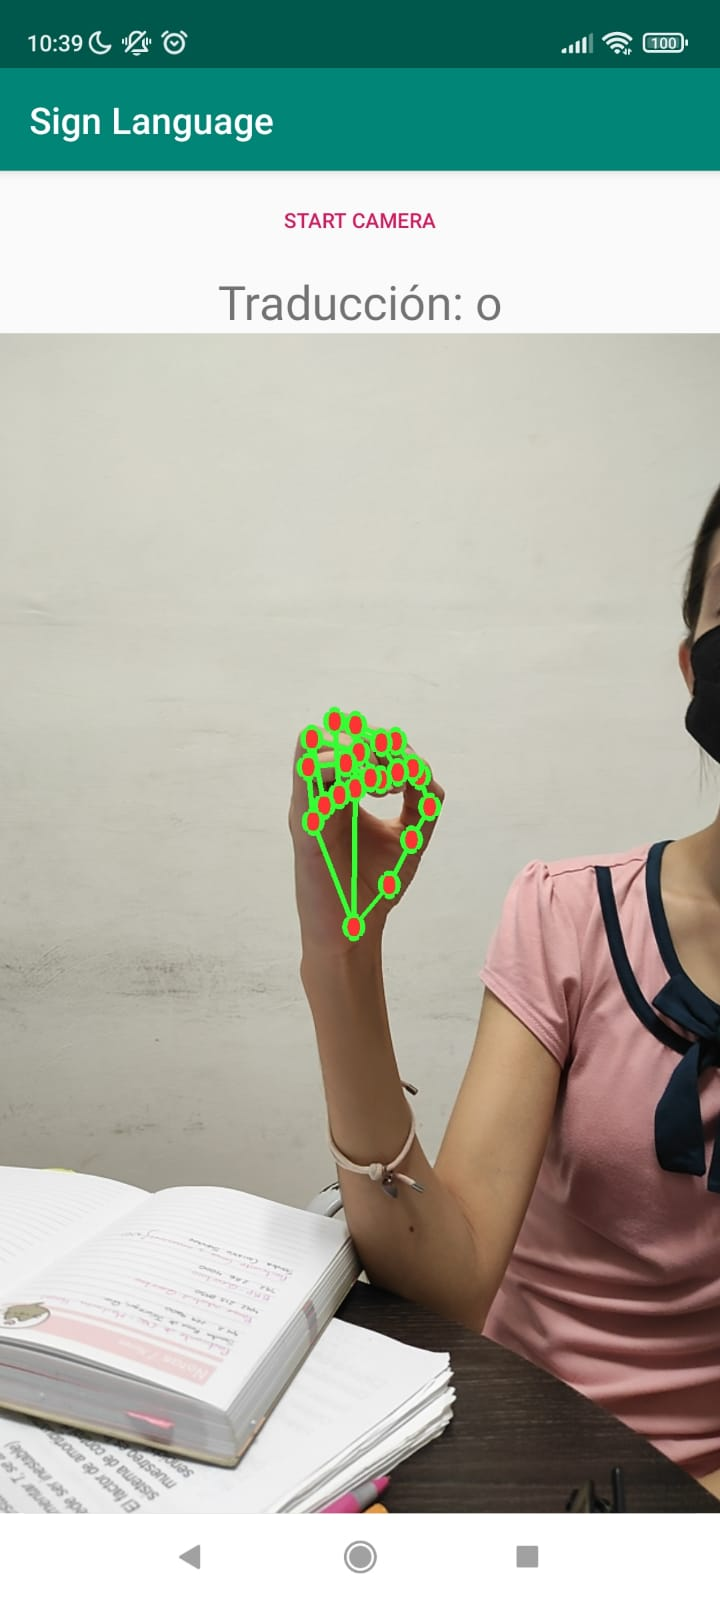
\includegraphics[width=0.16\textwidth]{2022_AplicacionLSM/figs/Muestra_compañeros2.jpeg}
  \end{tabular}
\end{center}

\end{frame}







%
\renewcommand{\EntradaBibtex}{MarcoNuno_ReportePaseLista_2022}

\begin{frame}{\citetitle{\EntradaBibtex} \footnotemark[1] (1)}
\begin{block}{Motivación} 
Es necesario una herramienta que permita al profesor pasar asistencia de manera ágil y rápida. 
\begin{itemize}
\item El profesor debe ingresar los grupos a partir de archivos de texto
\item El profesor ingresa a pase de lista y selecciona uno de sus grupos
\item Puede seleccionar asistencia a todos o falta a todos para agilizar el proceso
\item La aplicacion genera un informe con las estadisticas de asistencias, faltas y retartdos
\item Originalmente la lista se manejaba por archivos de texto, despues se migró a una base de datos SQLite
\end{itemize}
\end{block} 
\footnotetext[1]{\fullcite{\EntradaBibtex}}
\end{frame}


\begin{frame}{\citetitle{\EntradaBibtex} (2)}
%\begin{block}{Pantallas Principales} 
\begin{center}
	\begin{tabular}{cccc}
		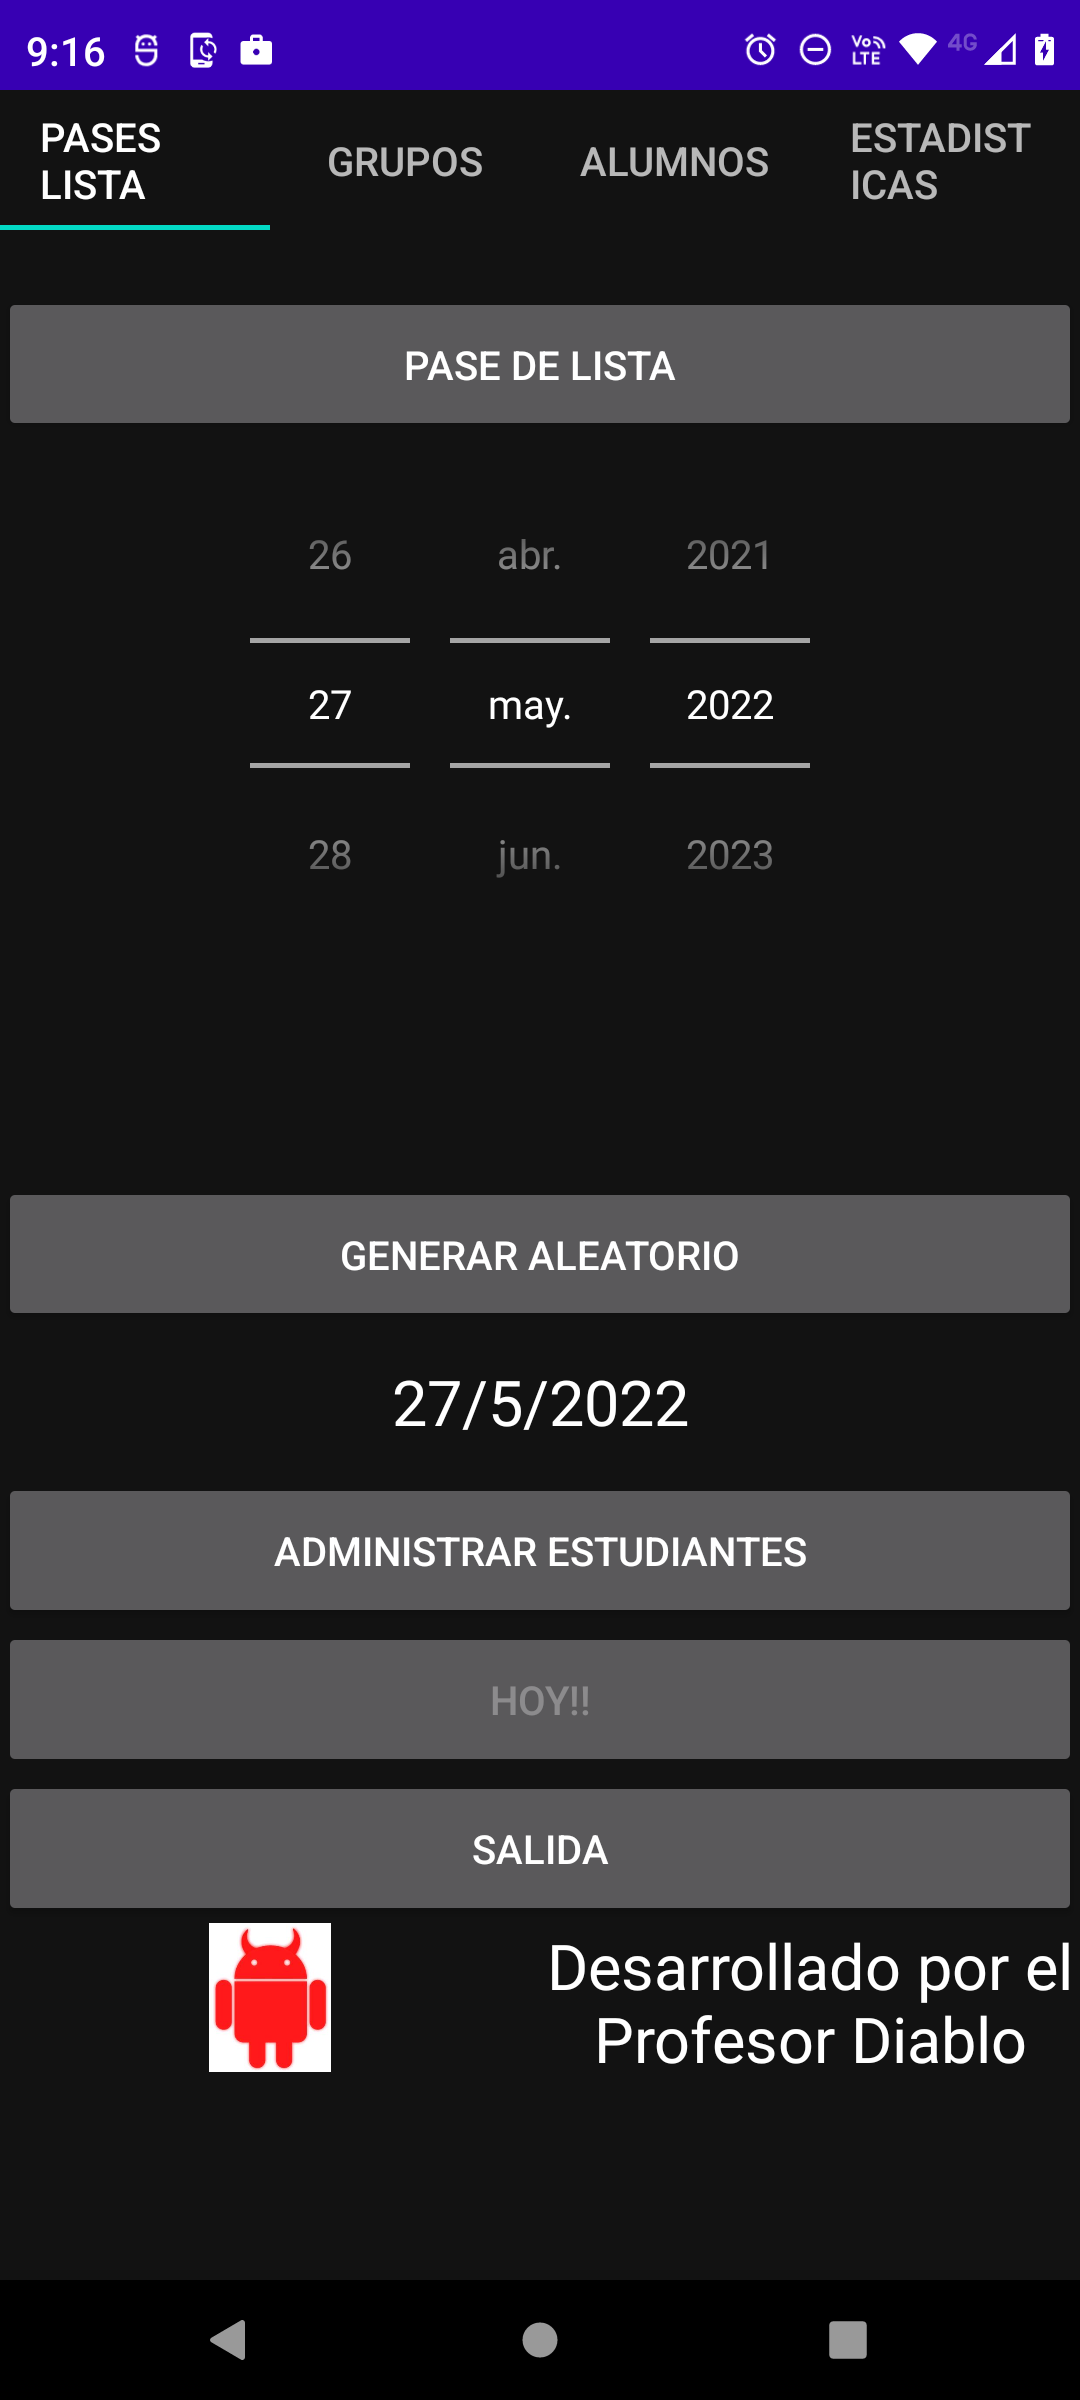
\includegraphics[width=0.20\linewidth]{2022_AppPaseLista/figs/PaseLista0.png} &
		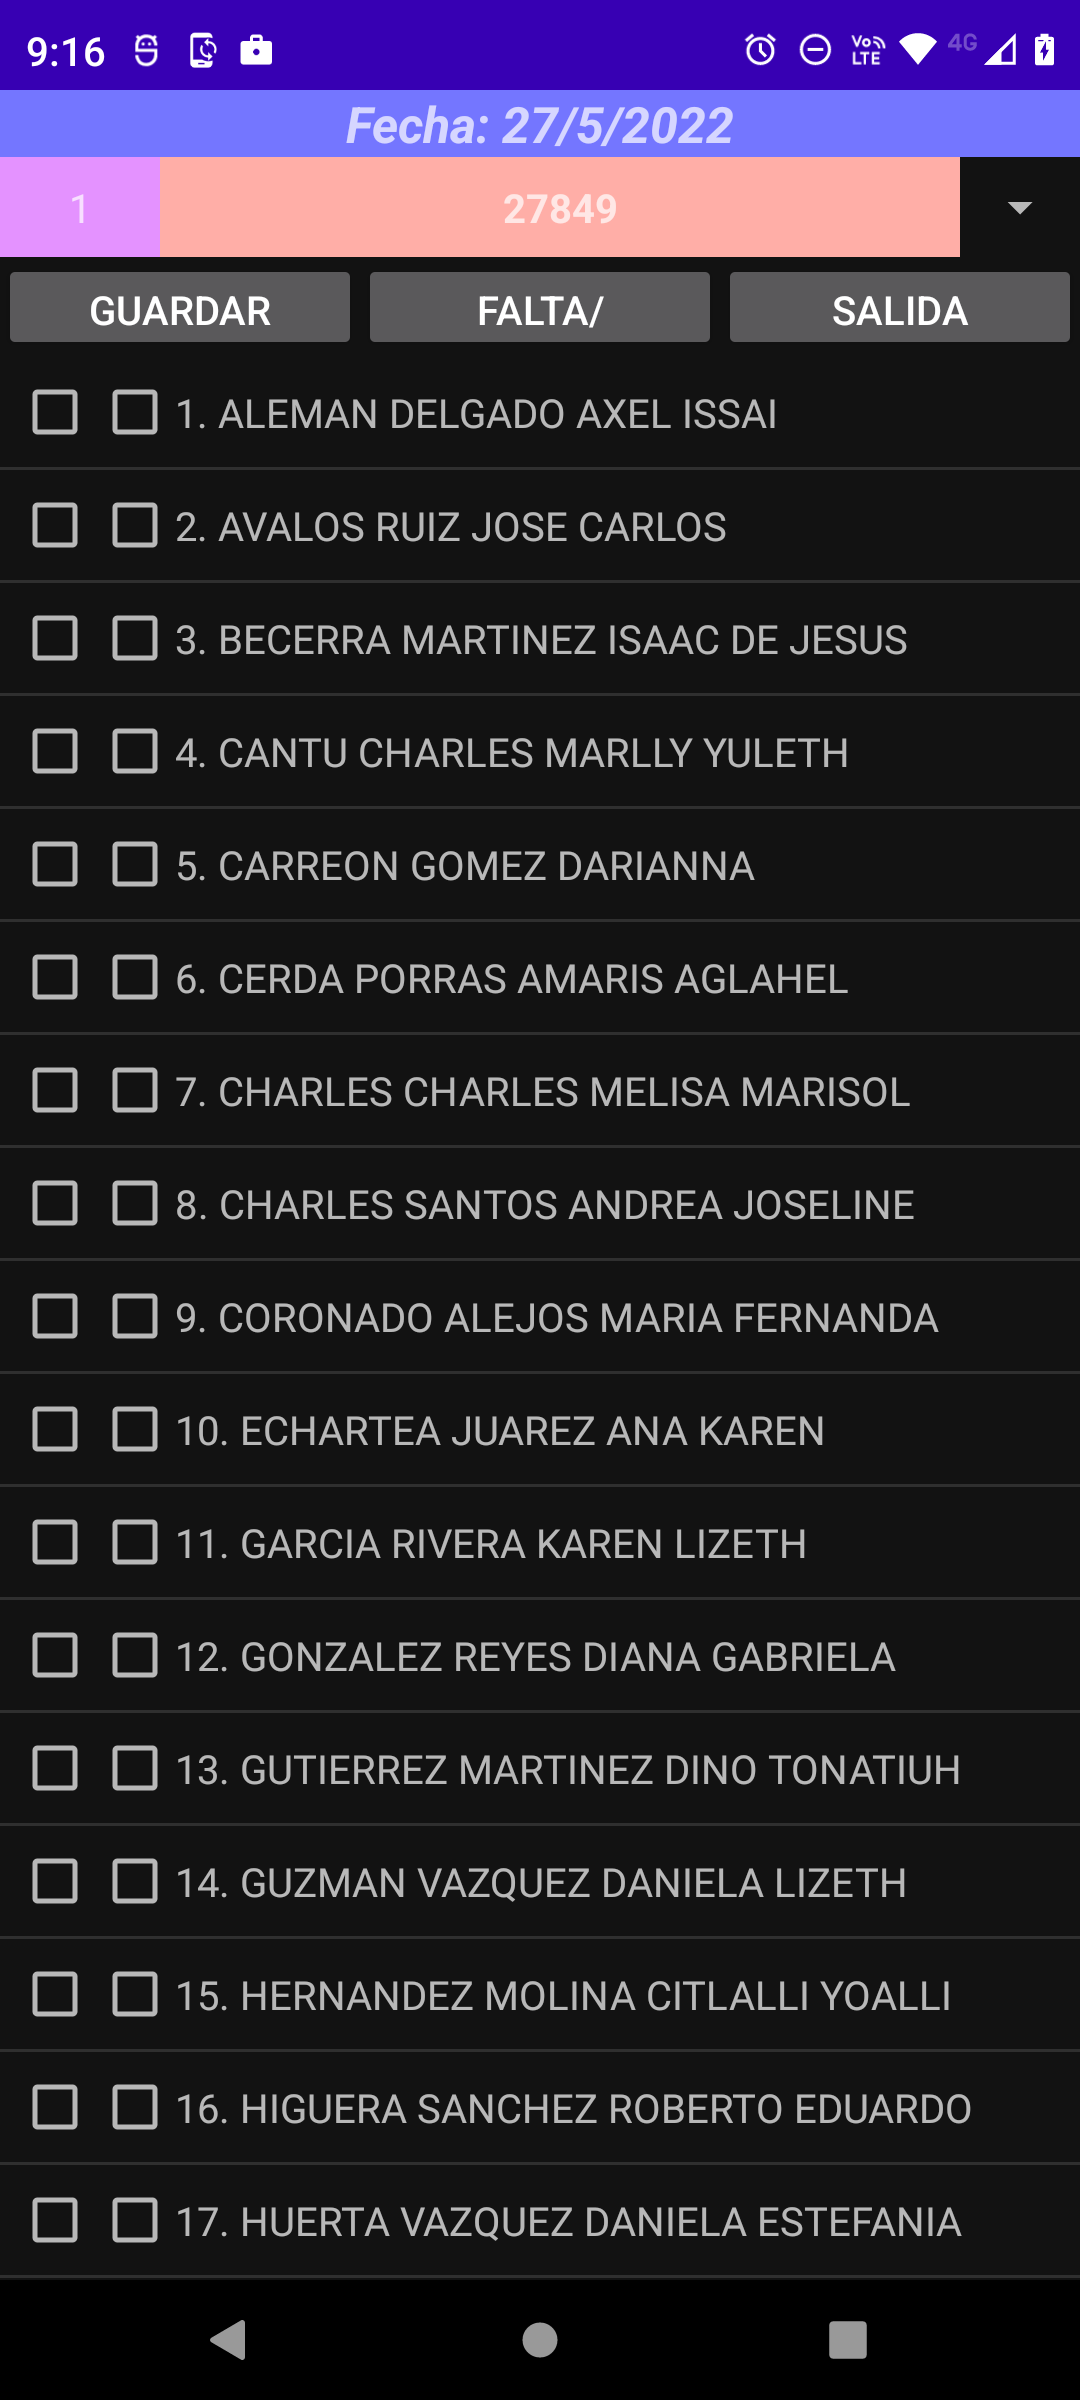
\includegraphics[width=0.20\linewidth]{2022_AppPaseLista/figs/PaseLista1.png} & 		 		
		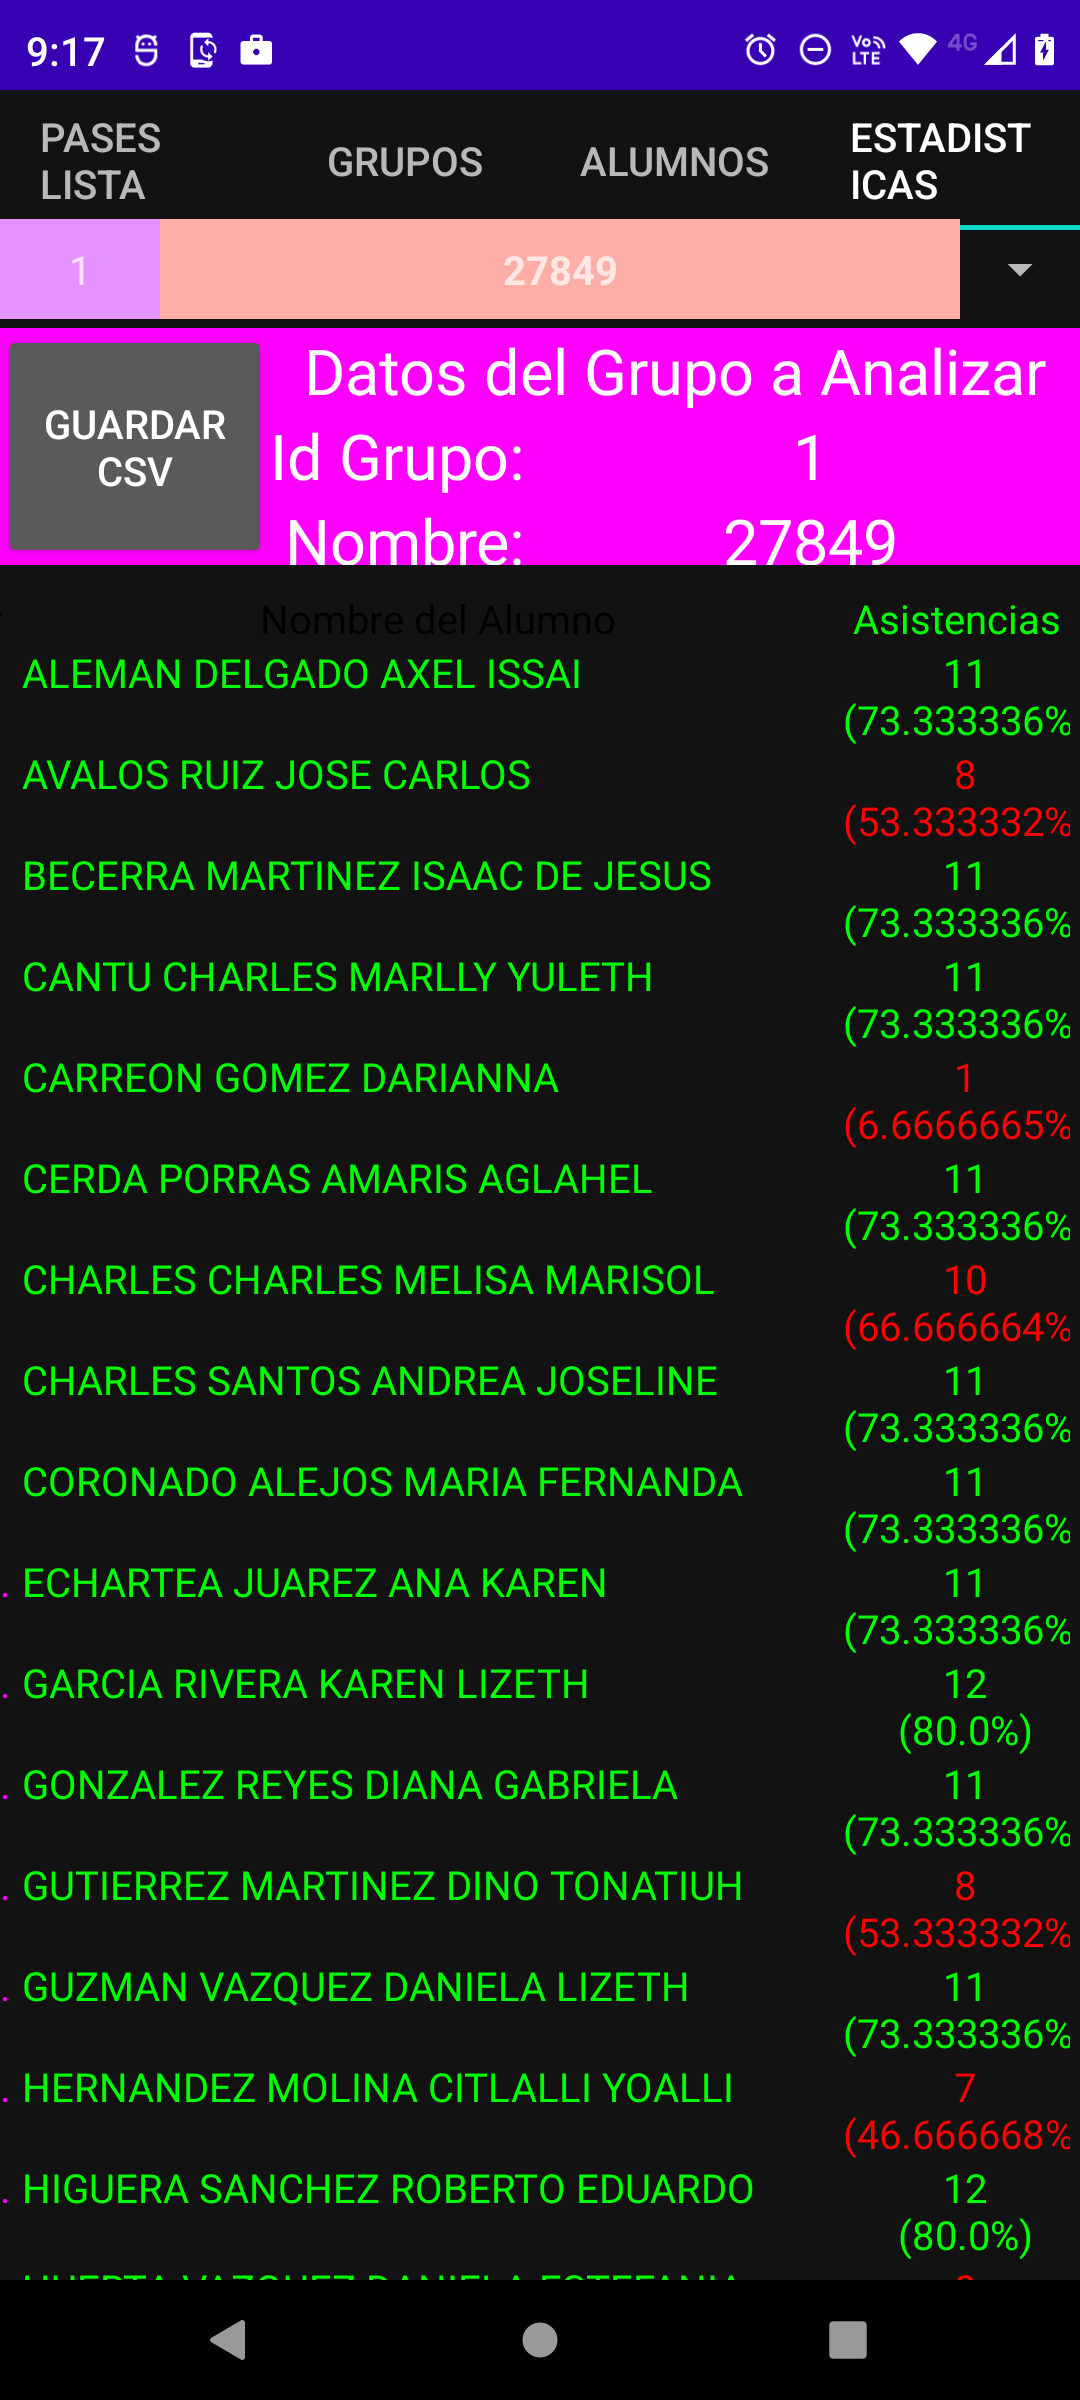
\includegraphics[width=0.20\linewidth]{2022_AppPaseLista/figs/PaseLista2.png} & 		
		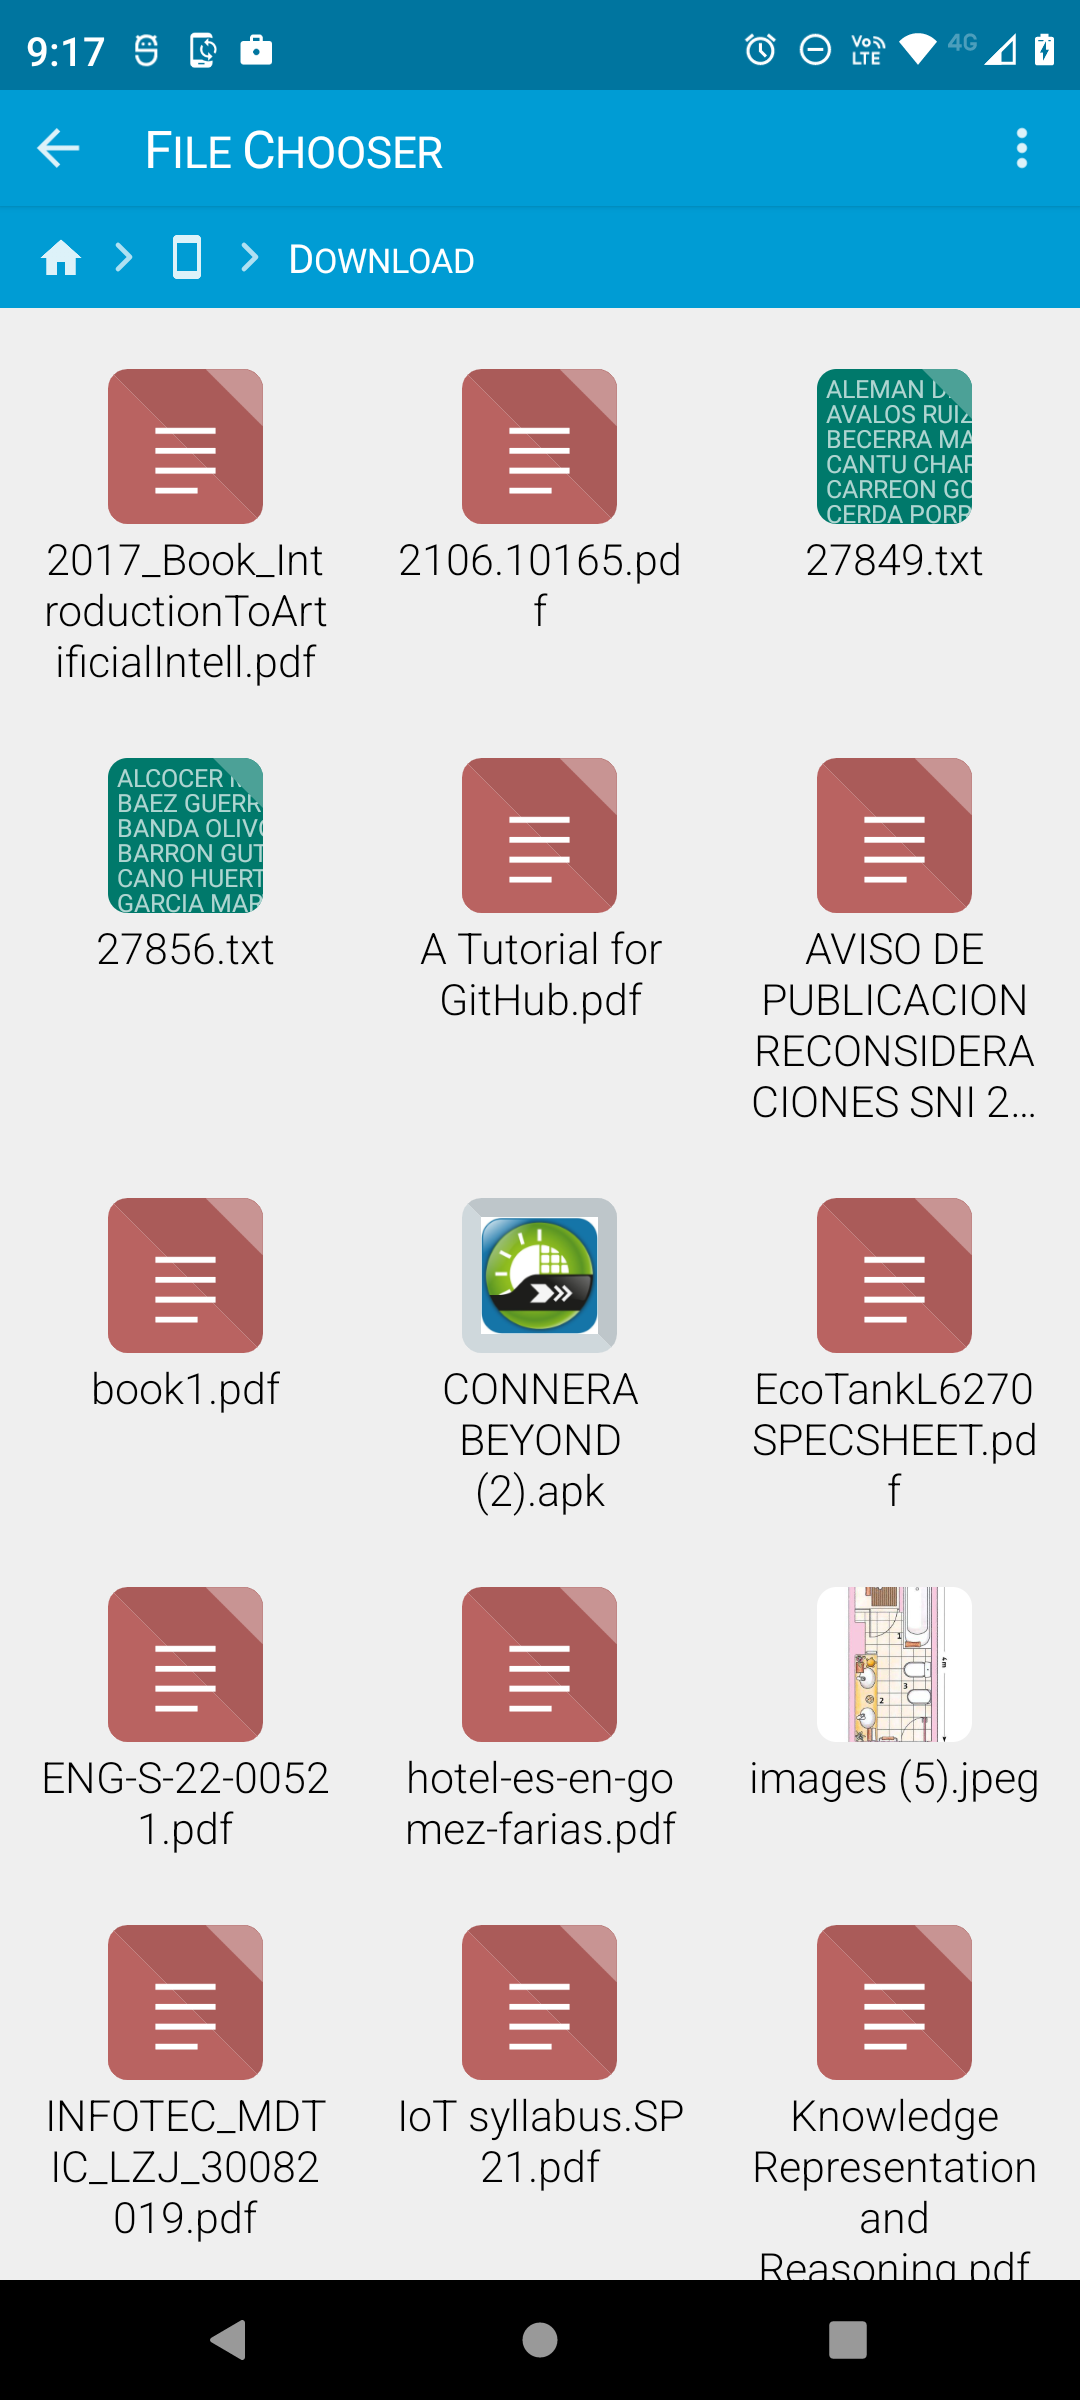
\includegraphics[width=0.20\linewidth]{2022_AppPaseLista/figs/PaseLista3.png} \\
	\end{tabular}
\end{center}
\end{frame}




%\renewcommand{\EntradaBibtex}{Froylan_VC_2021}

\begin{frame}{\citetitle{\EntradaBibtex} \footnotemark[1] (1)}


%\begin{frame}{Detección de movimientos en un tablero de ajedrez \footnotemark}
%\begin{block}{Detección de movimientos en un tablero de ajedrez \footnotemark} 
\begin{columns}
\begin{column}{0.38\textwidth}
Aplicación de escritorio:
	\begin{itemize}
\item Entorno semicontrolado con una cámara y una Laptop con OpenCV
\item Detecta las esquinas del tablero de ajedrez
\item Transformada de Hough
\item Detectar si hay casilla o no dentro de la región de interés
	\end{itemize}
\end{column}
\begin{column}{0.28\textwidth}
\begin{center}
     %%%%% this is a minipage, so \textwidth is already adjusted to the size of the column
     \includegraphics[width=0.75\textwidth]{Figs/AjedrezFroylan1}\\
%     \includegraphics[width=0.35\textwidth]{Figs/AjedrezFroylan2}
     \end{center}
\end{column}
\begin{column}{0.28\textwidth}
\begin{center}
     %%%%% this is a minipage, so \textwidth is already adjusted to the size of the column
 %    \includegraphics[width=0.35\textwidth]{Figs/AjedrezFroylan1}\\
     \includegraphics[width=0.75\textwidth]{Figs/AjedrezFroylan2}
     \end{center}
\end{column}

\end{columns}
%\end{block} 
\footnotetext[1]{\fullcite{\EntradaBibtex}}
%\footnotetext{Froylan Melquiades Wbario Martinez, \textbf{Seguidor de movimientos de Ajedrez}. Universidad Politécnica de Victoria, Informe técnico proyecto de asignatura “Visión por Computadora”, 2021.  En evaluación.}
%\\setcounter{footnote}{0}
\end{frame}

%\begin{frame}{Detección de movimientos en un tablero de ajedrez (2)}
\begin{frame}{\citetitle{\EntradaBibtex} (2)}
%\begin{block}{Detección de movimientos en un tablero de ajedrez (2)} 
\begin{columns}
\begin{column}{0.38\textwidth}
Aplicación de escritorio:
	\begin{itemize}
\item Una vez detectadas las regiones, se emplea un cronometro para determinar la diferencia entre dos instantaneas consecutivas
\item Problemas actuales: Iluminación, sombras, oclusiones
	\end{itemize}
\end{column}
\begin{column}{0.28\textwidth}
\begin{center}
     %%%%% this is a minipage, so \textwidth is already adjusted to the size of the column
     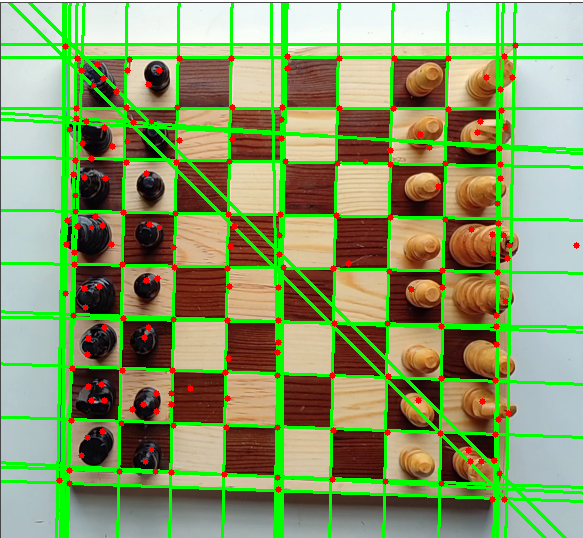
\includegraphics[width=0.79\textwidth]{Figs/AjedrezFroylan3}\\
%     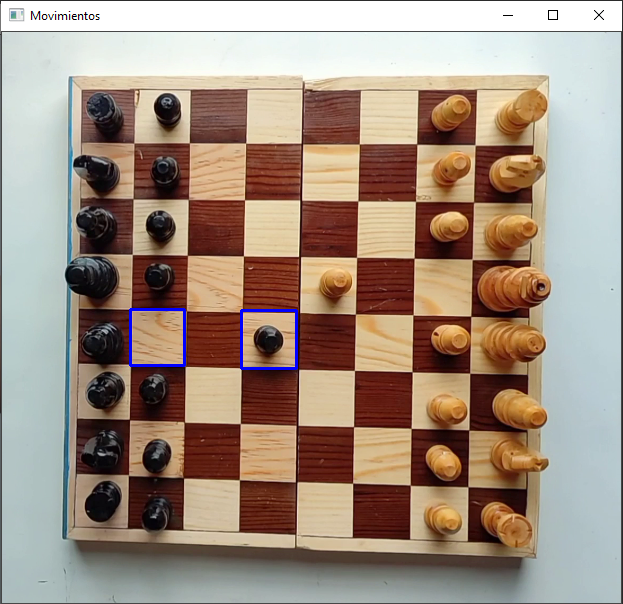
\includegraphics[width=0.49\textwidth]{Figs/AjedrezFroylan4}
     \end{center}
\end{column}
\begin{column}{0.28\textwidth}
\begin{center}
     %%%%% this is a minipage, so \textwidth is already adjusted to the size of the column
%     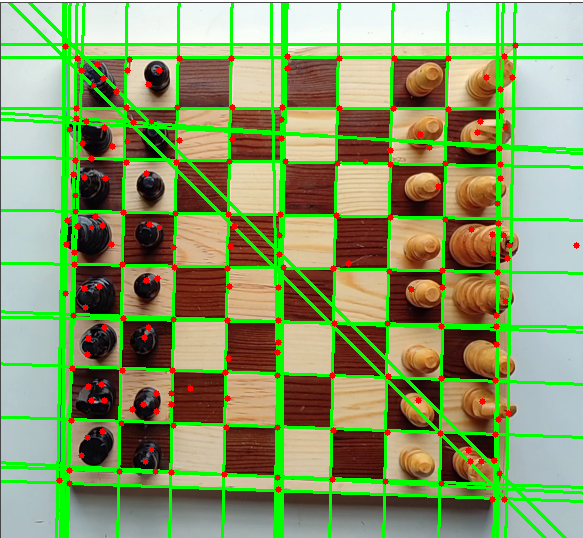
\includegraphics[width=0.49\textwidth]{Figs/AjedrezFroylan3}\\
     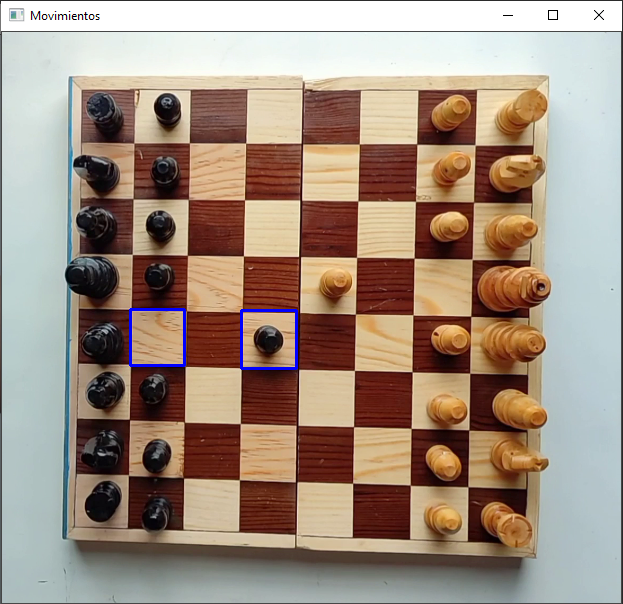
\includegraphics[width=0.79\textwidth]{Figs/AjedrezFroylan4}
     \end{center}
\end{column}

\end{columns}
%\end{block} 
\end{frame}


%
%\begin{frame}{\citetitle{MarcoNuno_Revista_2021_10_00}$^*$  (1)}
\renewcommand{\EntradaBibtex}{MarcoNuno_Revista_2021_10_00}

\begin{frame}{\citetitle{\EntradaBibtex} \footnotemark[1] (1)}

\begin{columns}
\begin{column}{0.70\textwidth}
	\begin{itemize}
		\item Se propone un protitipo para monitorear de manera remota temperatura y humedad
        \item Aplicaciones particulares: cultivos (tradicionales, invernaderos, sistemas hidropónicos o acuapónicos, etc)
		\item El sensor estan enviando información utilizando el protocolo MQTT y un servidor especializado (Broker)
        \item Se implementó una aplicación móvil que muestra notificaciones y estadísticas del comportamiento de dichas variables
	\end{itemize}
\end{column}
\begin{column}{0.30\textwidth}  
\begin{center}
     \begin{tabular}{cc}
         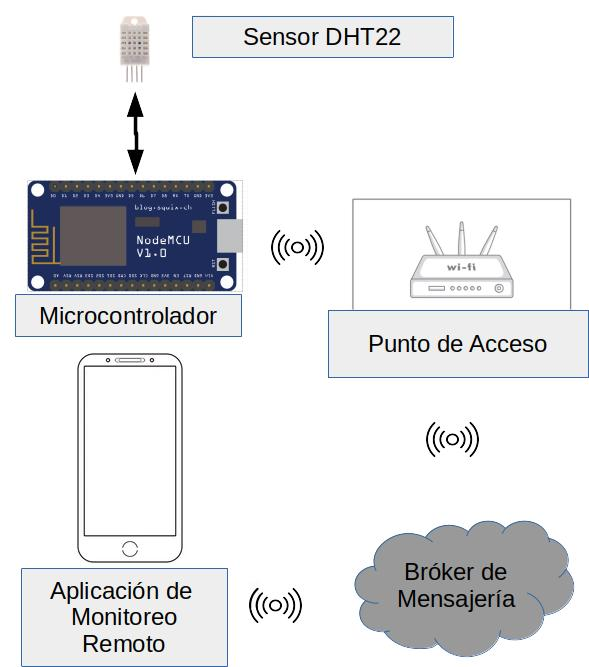
\includegraphics[width=0.98\textwidth]{2021_IoT_JoseRamon/figs/Figura_Refrigeradores.jpg}\\         
      \end{tabular}
\end{center}
\end{column} 
\end{columns} 


%\footnotetext[1]{\fullcite{MarcoNuno_ReporteTecnico2022_C}}
%\setcounter{footnote}{0}
\footnotetext[1]{\fullcite{\EntradaBibtex}}
\end{frame}



\begin{frame}{\citetitle{\EntradaBibtex} (2)}
\begin{columns}
\begin{column}{0.40\textwidth}
Componentes hardware:
\begin{itemize}
    \item Tarjeta Nodemcu Esp8266 WiFi. 
    \item Sensor de Humedad/Temperatura DHT22, alimentado por el NodeMCU, con una mayor precisón en comparación con su predesor el DTH22
    \item Router para conectividad remota a internet
	\end{itemize}
\end{column}
\begin{column}{0.60\textwidth}  
\begin{center}
     \begin{tabular}{c}
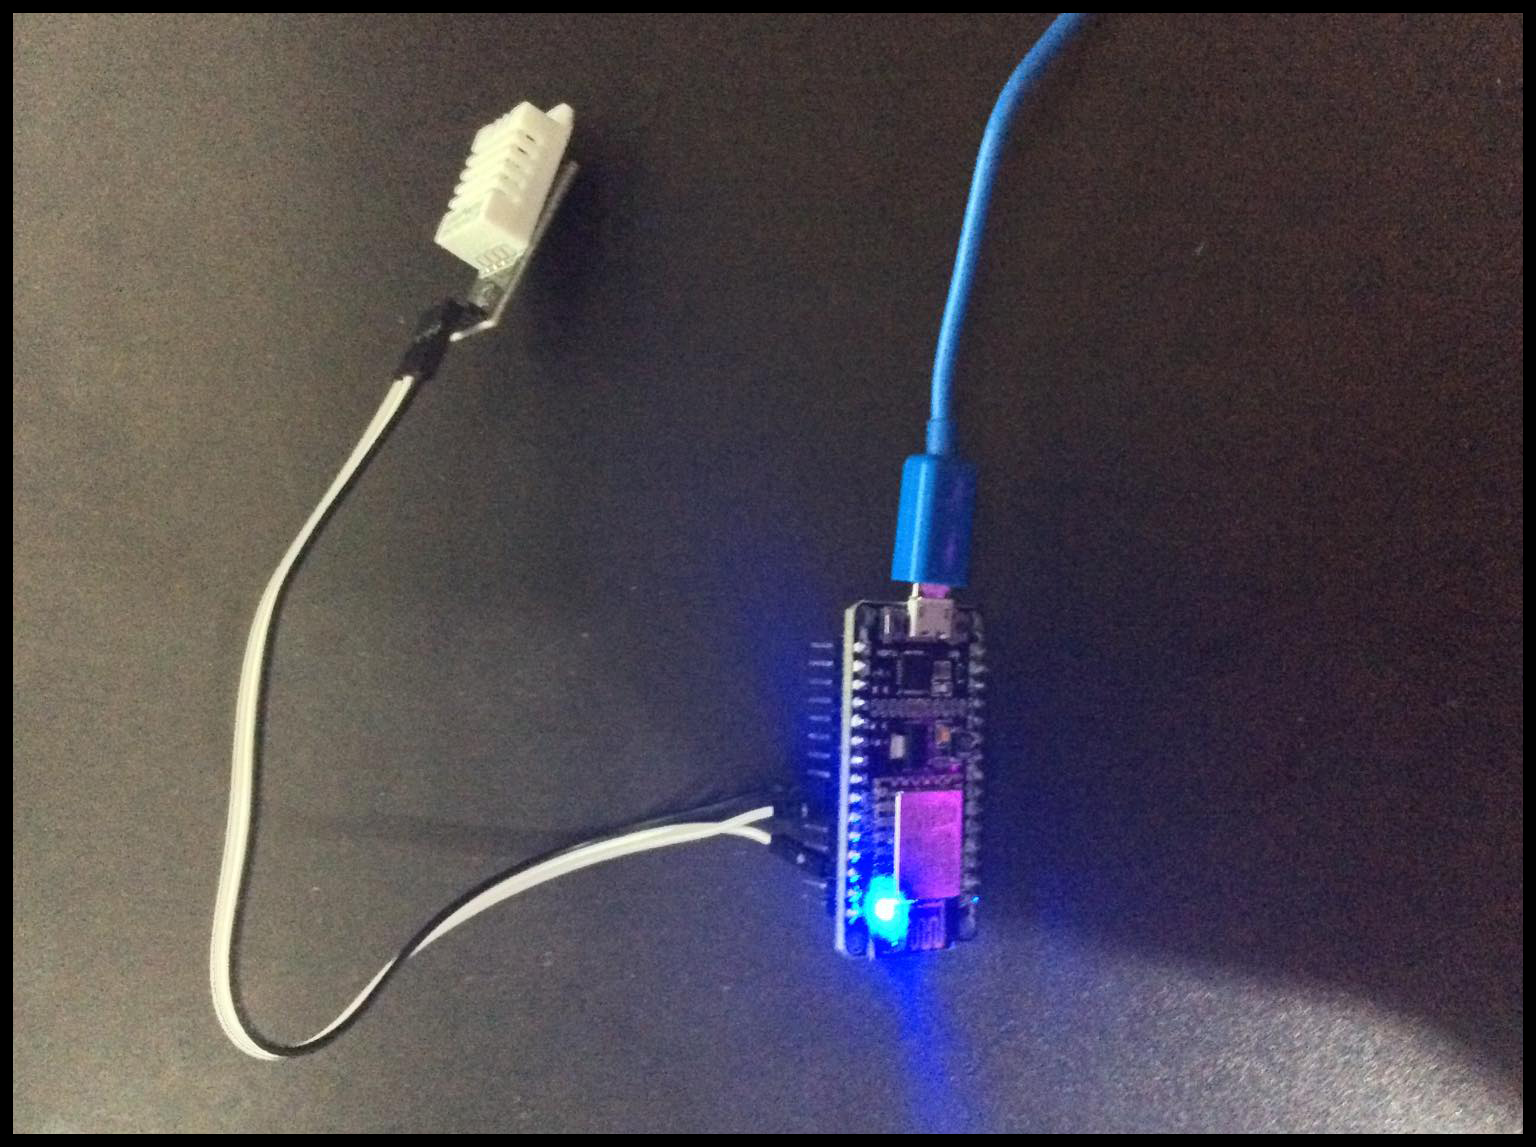
\includegraphics[width=0.48\textwidth]{2021_IoT_JoseRamon/figs/resultadodelsensor.jpg}
\includegraphics[width=0.48\textwidth]{2021_IoT_JoseRamon/figs/image.png}\\
          \end{tabular}
\end{center}
\end{column} 
\end{columns} 
\end{frame}



\begin{frame}{\citetitle{\EntradaBibtex} (3)}
\begin{columns}
\begin{column}{0.40\textwidth}
La aplicación movil desarrollada tiene las siguientes funcionalidades:
\begin{itemize}
        \item Permite configurar los datos de conectividad con el Broker
        \item Establece parámetros de las alarmas y notificaciones
        \item Permite visualizar datos de manera gráfica
	\end{itemize}
\end{column}
\begin{column}{0.60\textwidth}  
\begin{center}
     \begin{tabular}{c}
         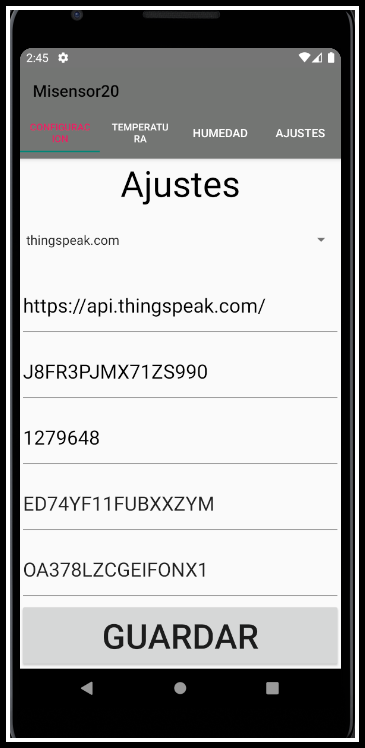
\includegraphics[width=0.32\textwidth]{2021_IoT_JoseRamon/figs/pantalla de configuracion.png}
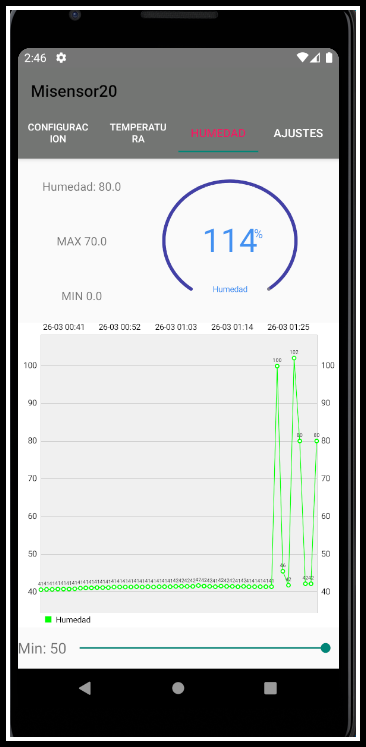
\includegraphics[width=0.32\textwidth]{2021_IoT_JoseRamon/figs/pantalla de humedad.png}
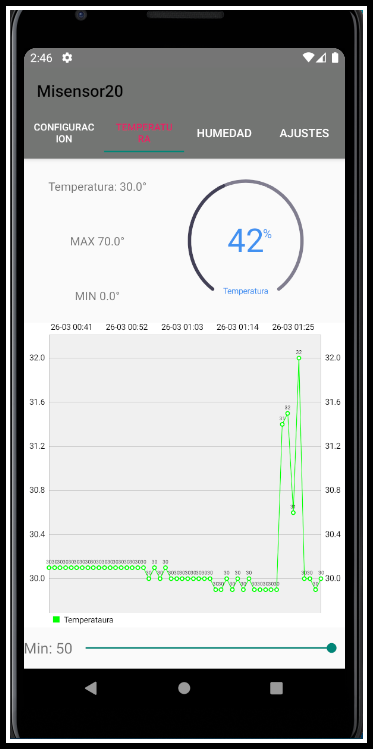
\includegraphics[width=0.32\textwidth]{2021_IoT_JoseRamon/figs/pantalla de temperatura.png}\\

          \end{tabular}
\end{center}
\end{column} 
\end{columns} 
\end{frame}



\begin{frame}{\citetitle{\EntradaBibtex} (4)}
\begin{columns}
\begin{column}{0.40\textwidth}
\begin{itemize}
        \item Una vez que la aplicación ha sido configurada, dependiendo de los umbrales establecidos, se emite una notificación al usuario cuando se rebazan dichos umbrales
        \item Esto permite detectar problemas y/o tomar acciones correctivas
	\end{itemize}
\end{column}
\begin{column}{0.60\textwidth}  
\begin{center}
     \begin{tabular}{c}
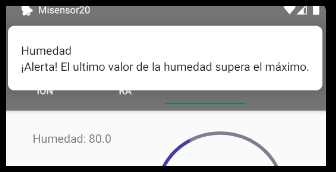
\includegraphics[width=0.48\textwidth]{2021_IoT_JoseRamon/figs/Alerta humedad.png}
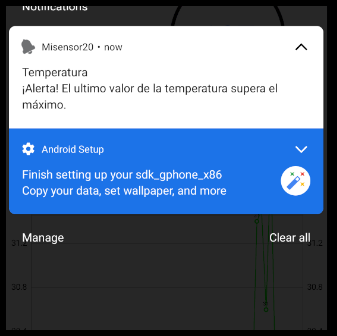
\includegraphics[width=0.48\textwidth]{2021_IoT_JoseRamon/figs/Alerta Temperatura.png}\\
          \end{tabular}
\end{center}
\end{column} 
\end{columns} 
\end{frame}







%\renewcommand{\EntradaBibtex}{TutorialBlender_Lazo_2020}

\begin{frame}{\citetitle{\EntradaBibtex} \footnotemark[1] (1)}

%\begin{frame}{Tutorial del uso de Blender \footnotemark}
%\begin{block}{Tutorial del uso de Blender \footnotemark} 
\begin{columns}
\begin{column}{0.23\textwidth}
    \begin{center}
	    \begin{tabular}{c}
		        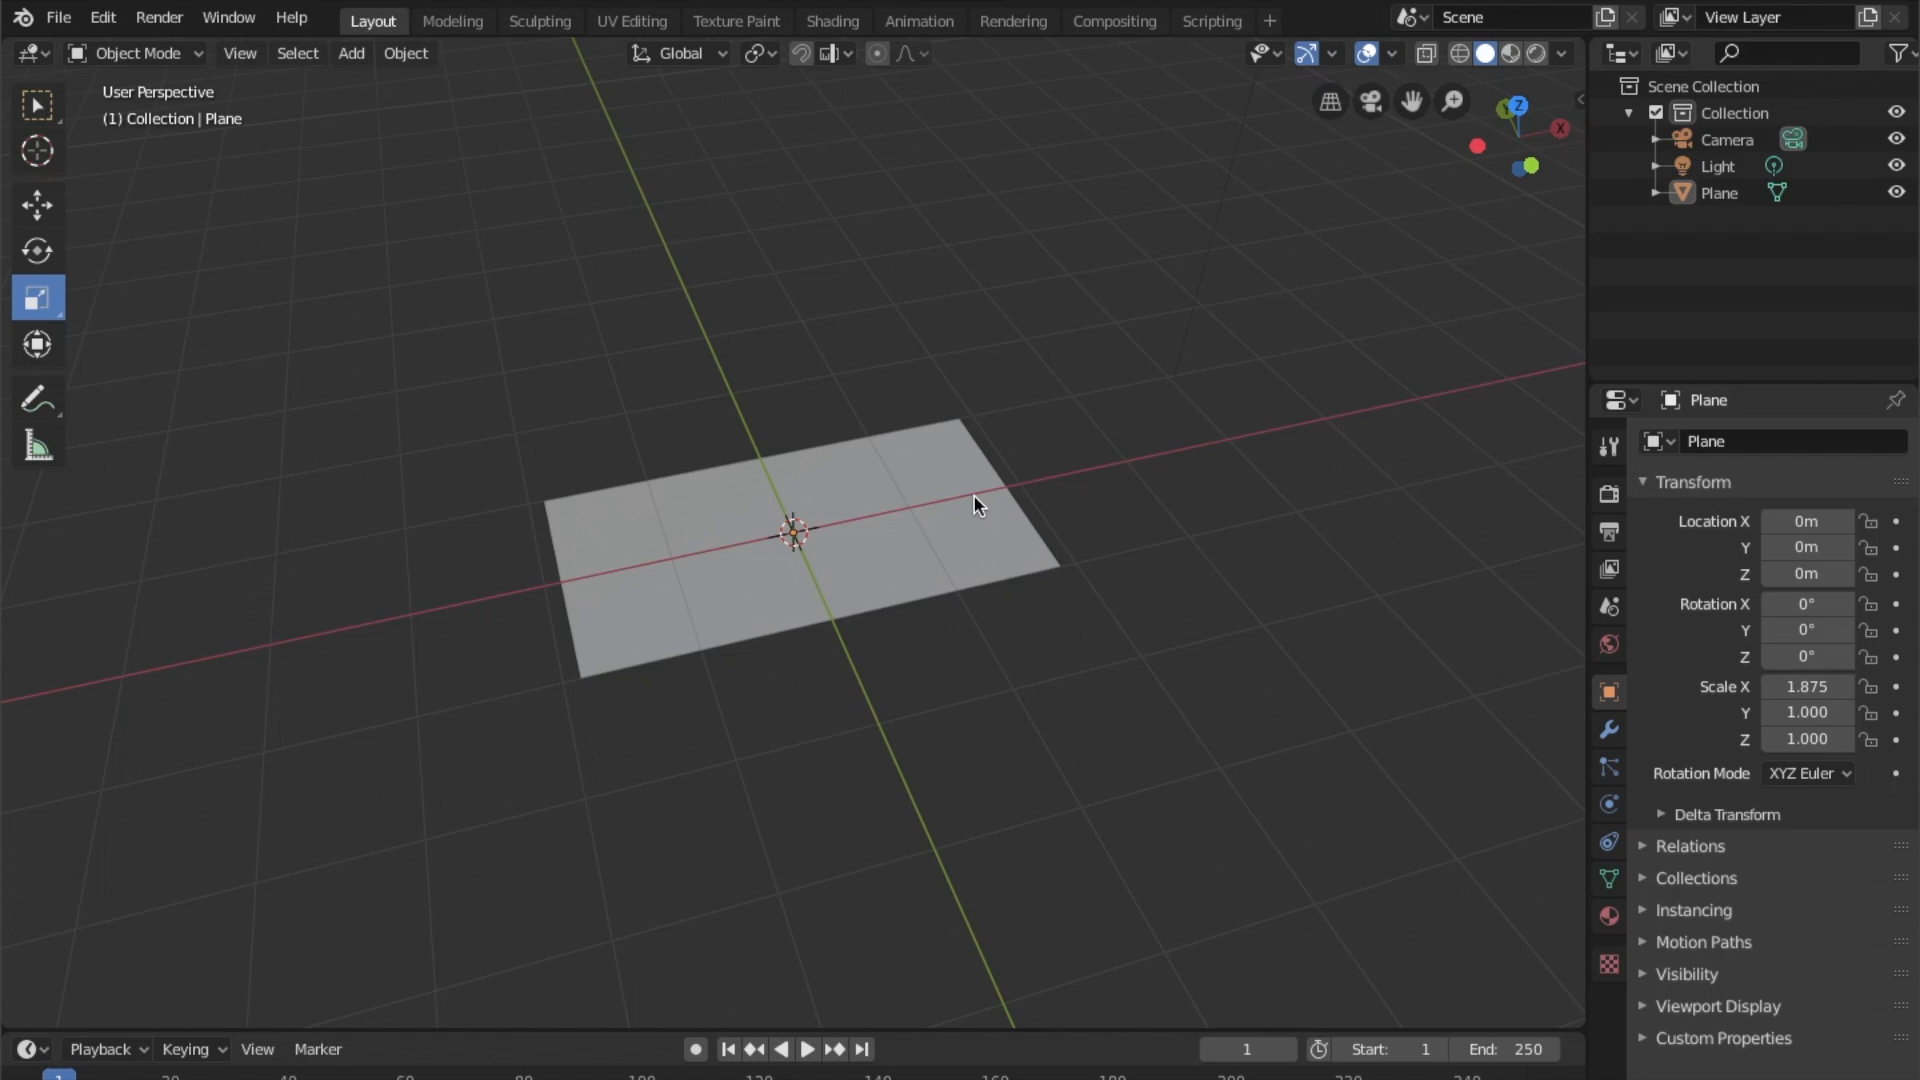
\includegraphics[width=0.75\linewidth]{Figs/VideoBlender01}\\
		        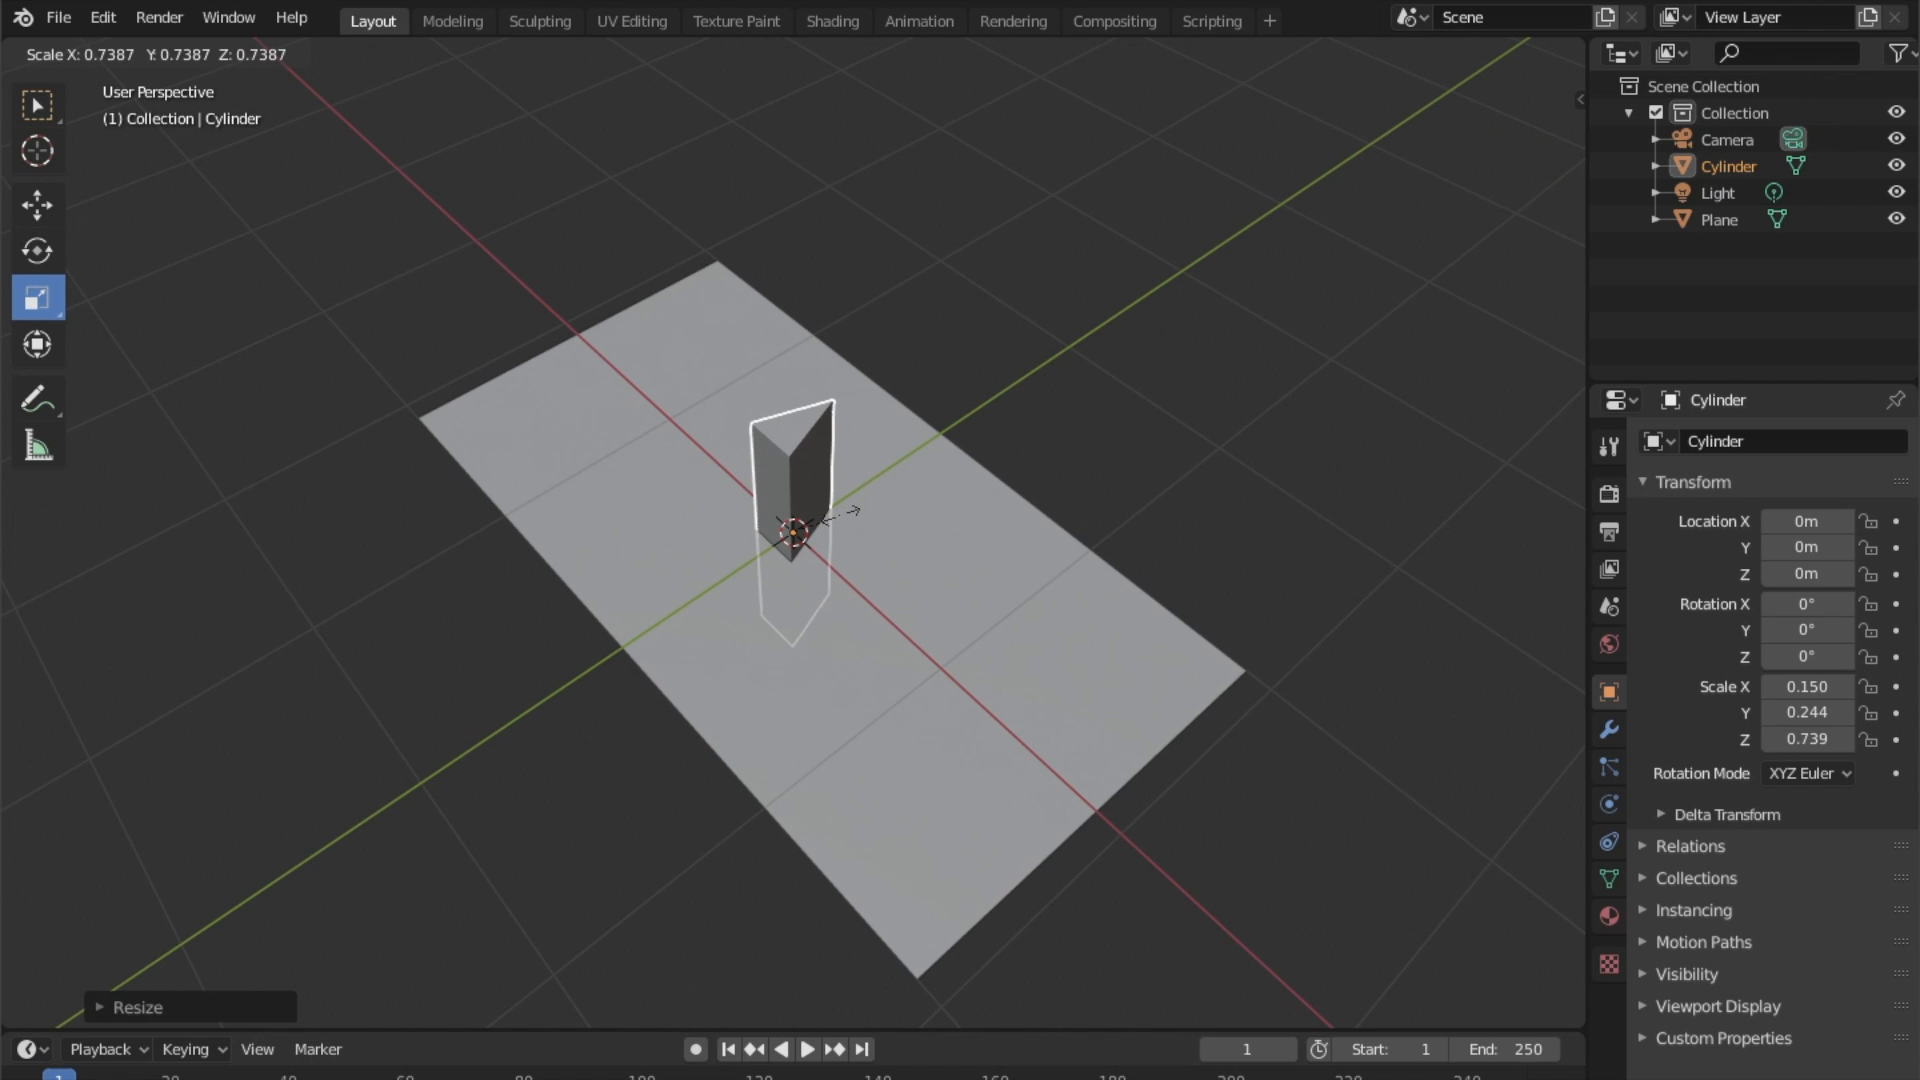
\includegraphics[width=0.75\linewidth]{Figs/VideoBlender02}\\
                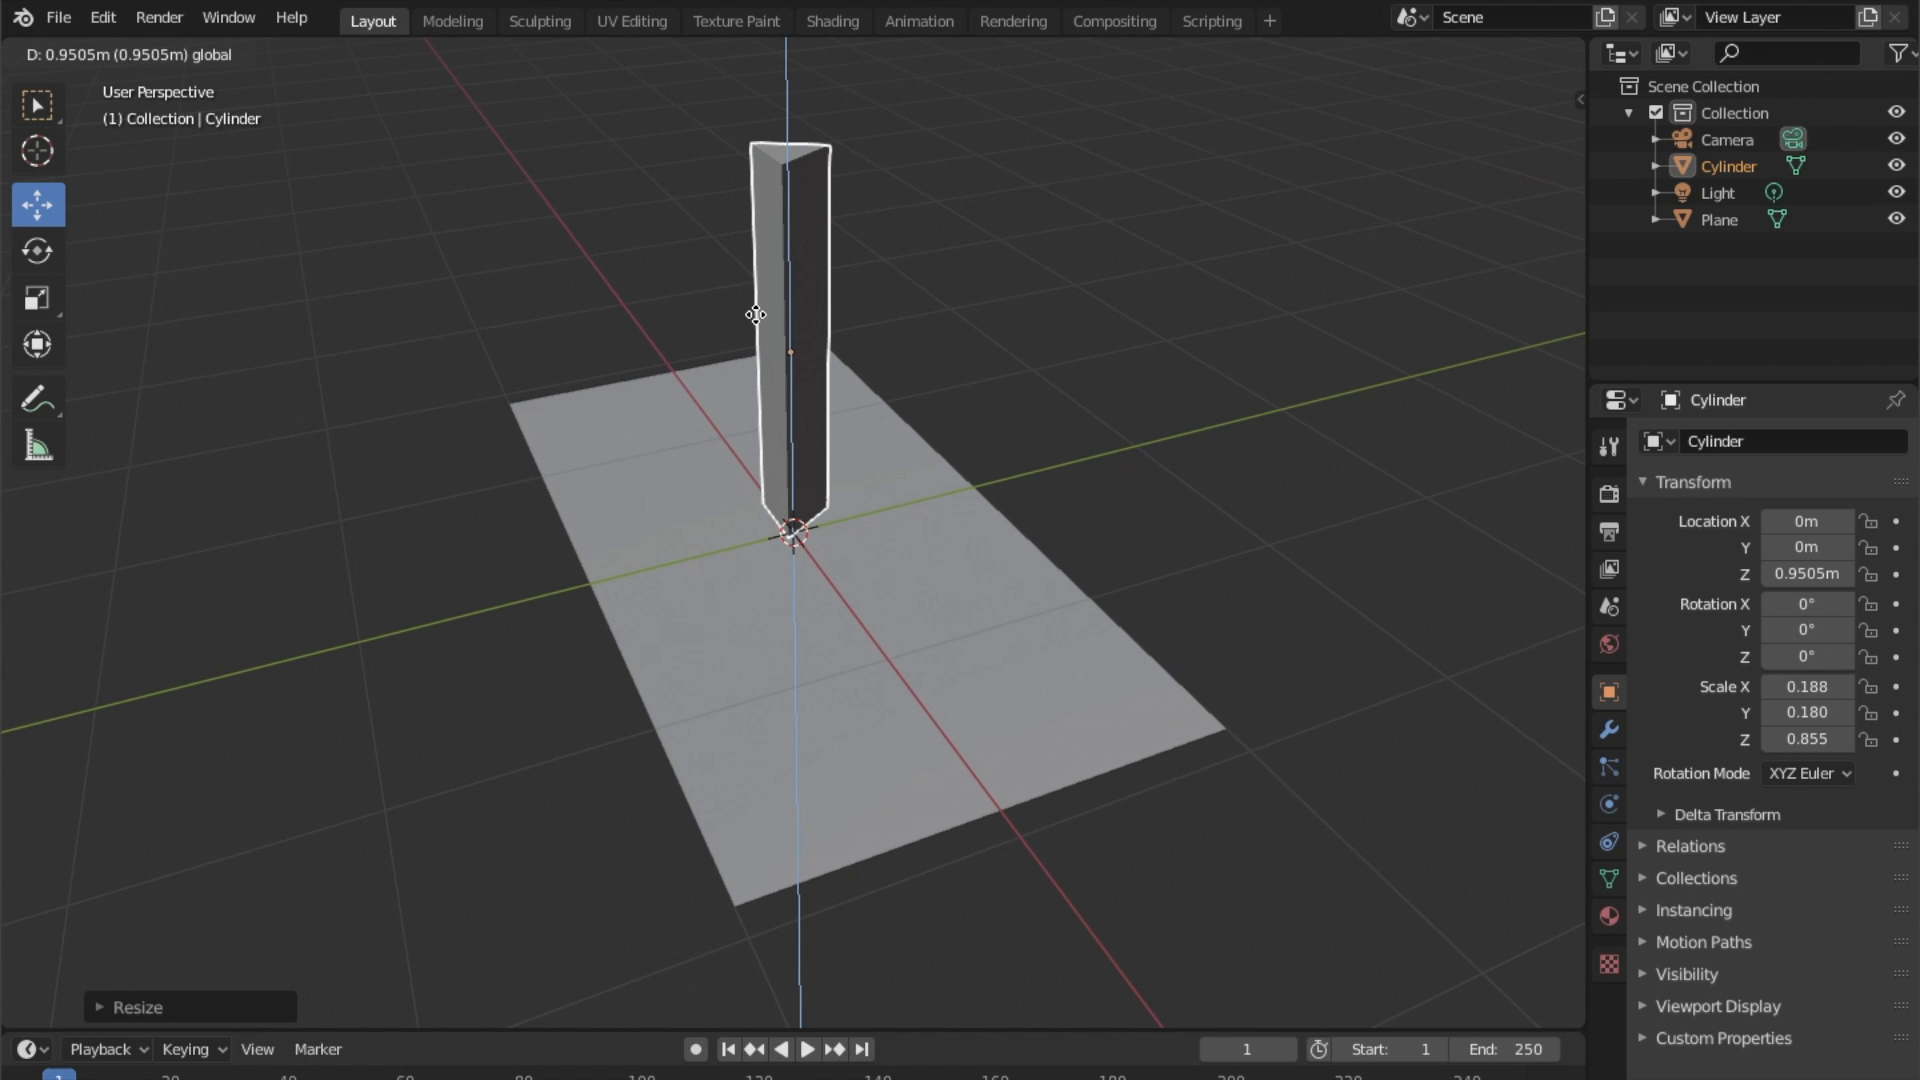
\includegraphics[width=0.75\linewidth]{Figs/VideoBlender03}\\
	    \end{tabular}
    \end{center}
\end{column}
\begin{column}{0.23\textwidth}
    \begin{center}
	    \begin{tabular}{c}
		        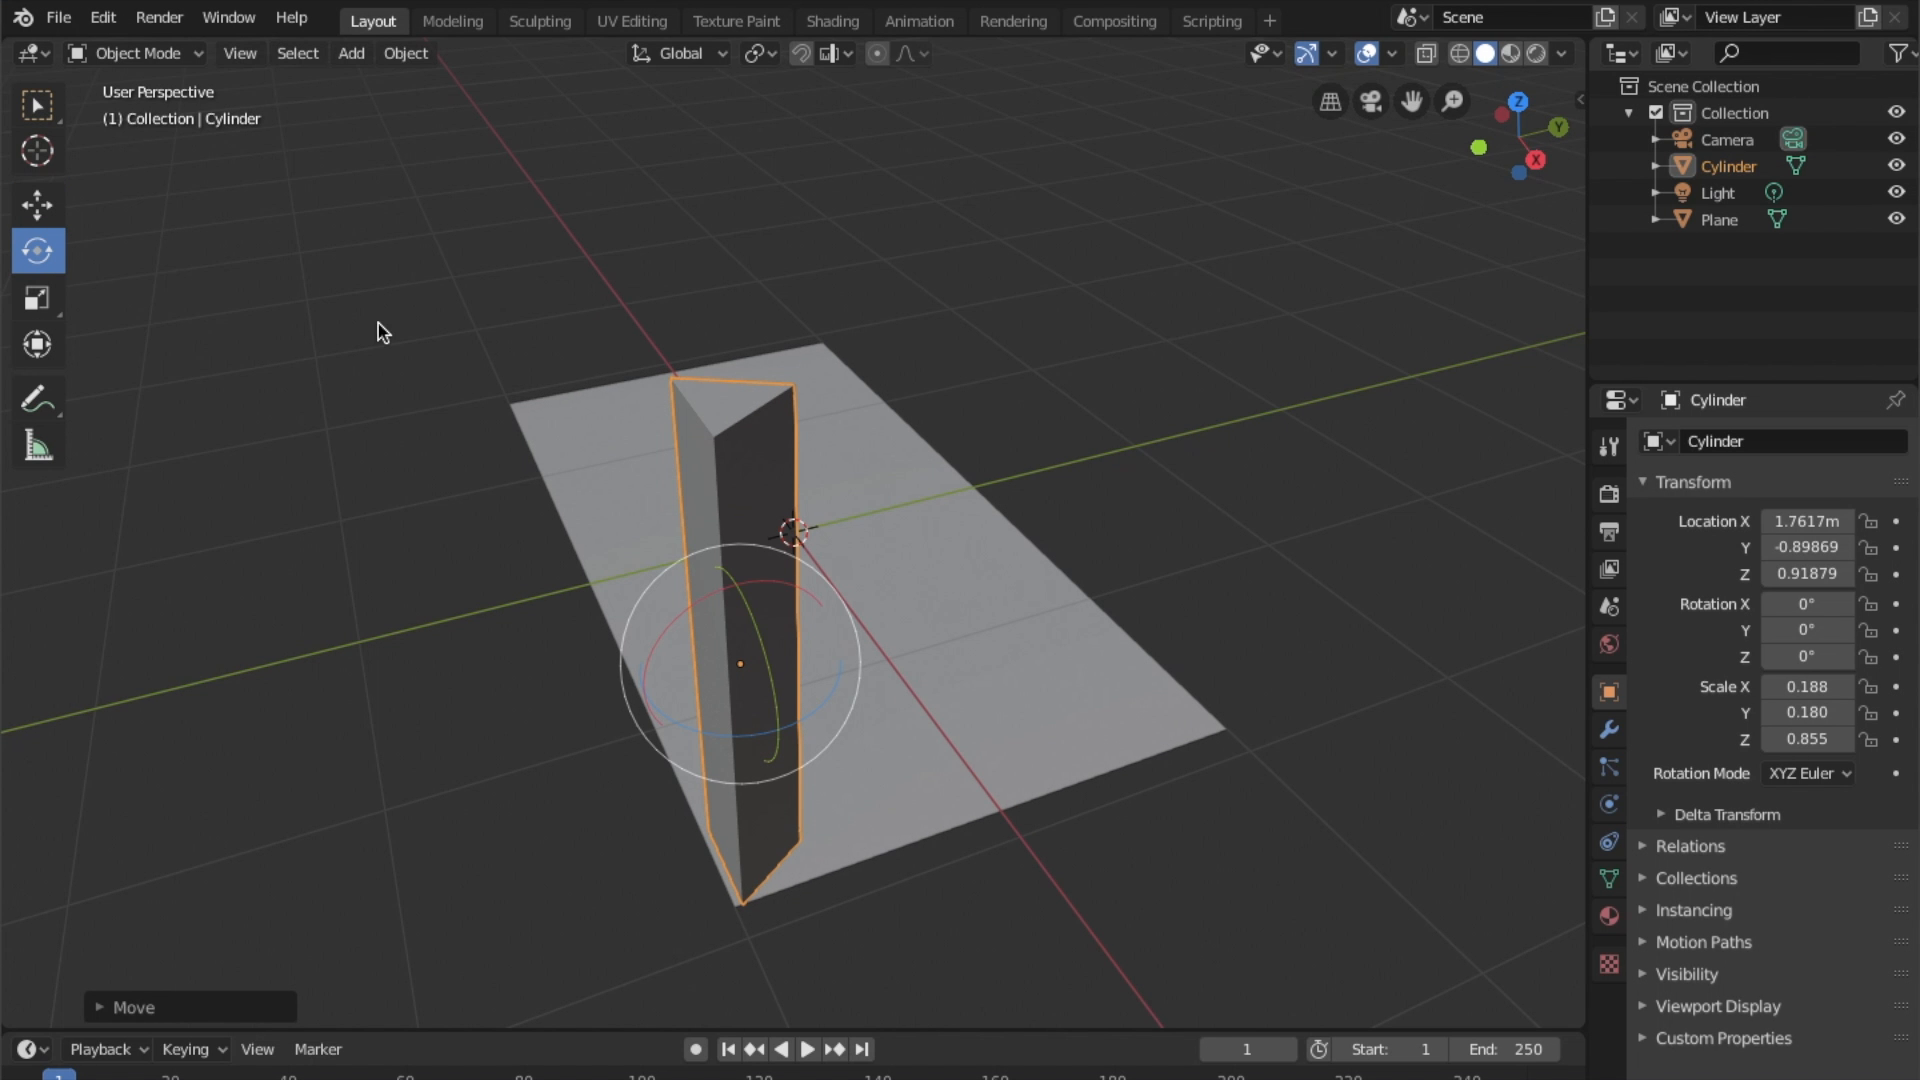
\includegraphics[width=0.75\linewidth]{Figs/VideoBlender04}\\
		        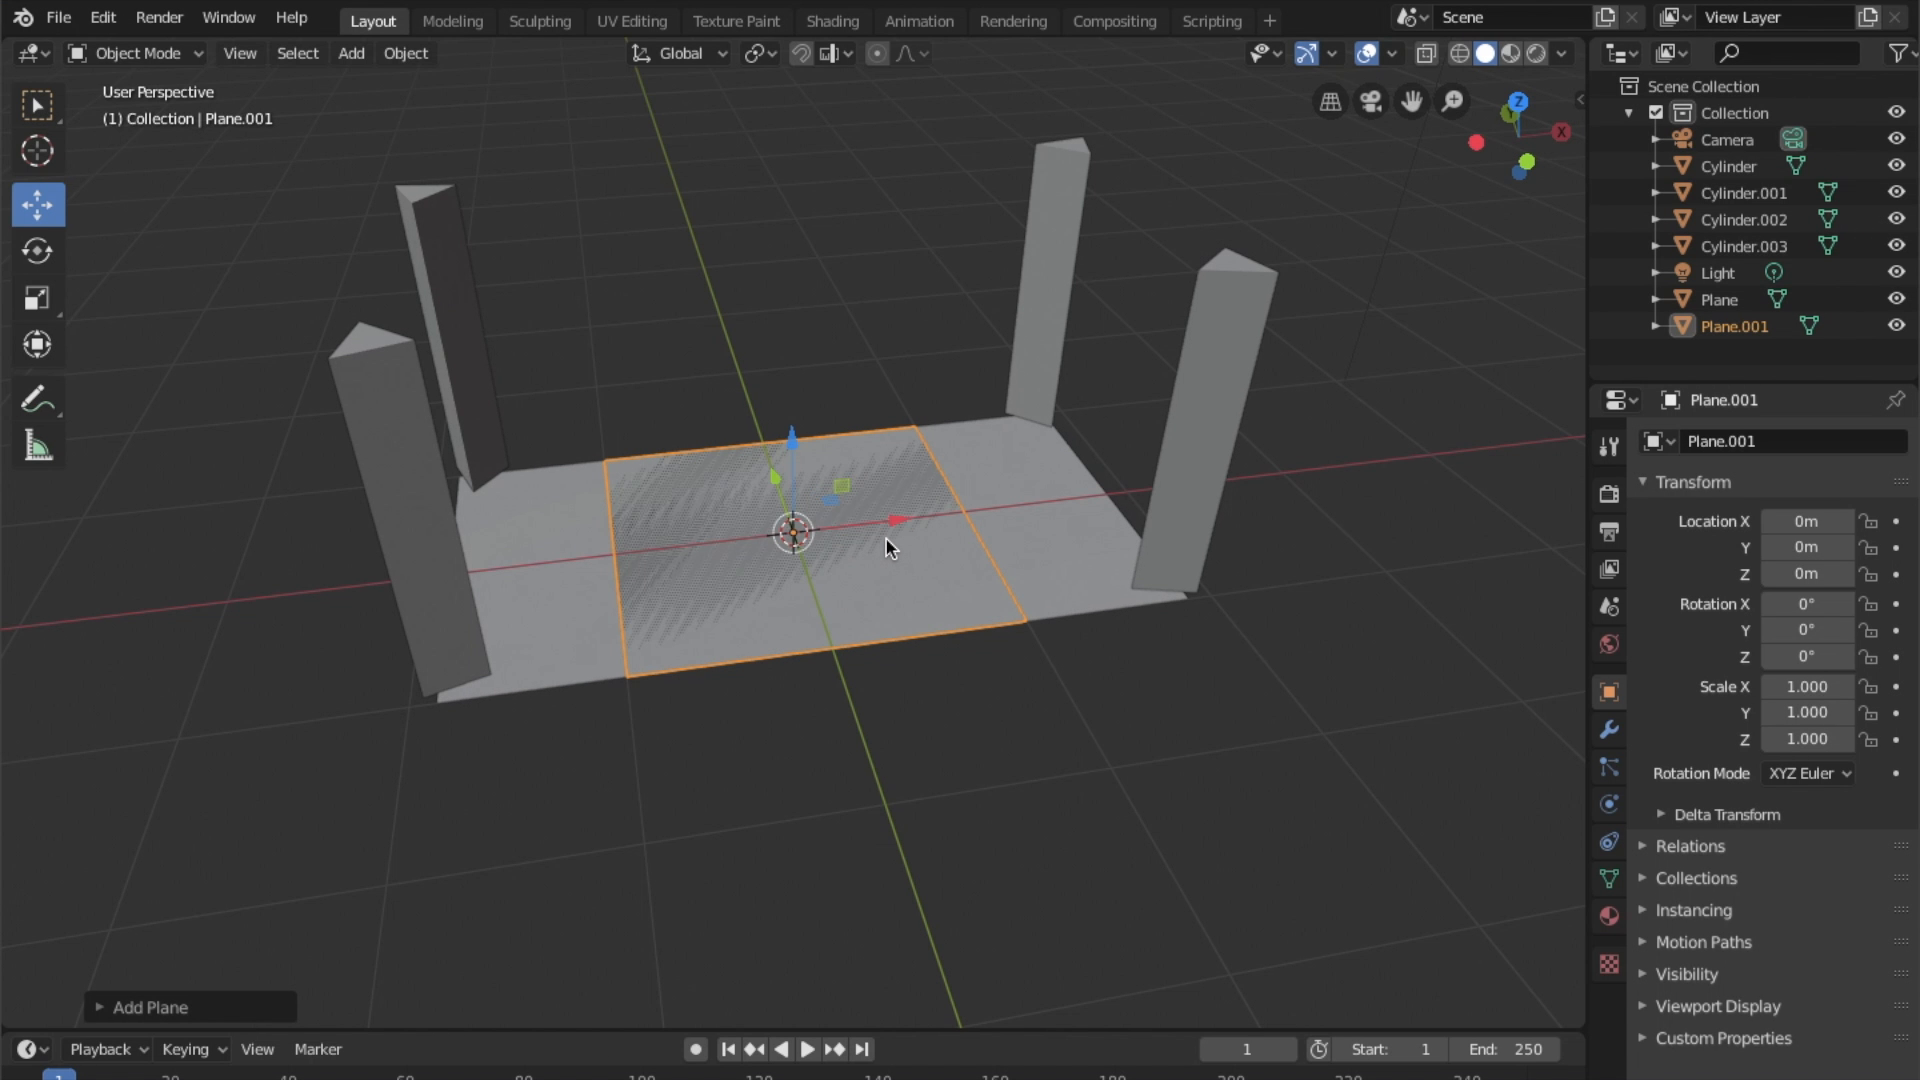
\includegraphics[width=0.75\linewidth]{Figs/VideoBlender05}\\
		        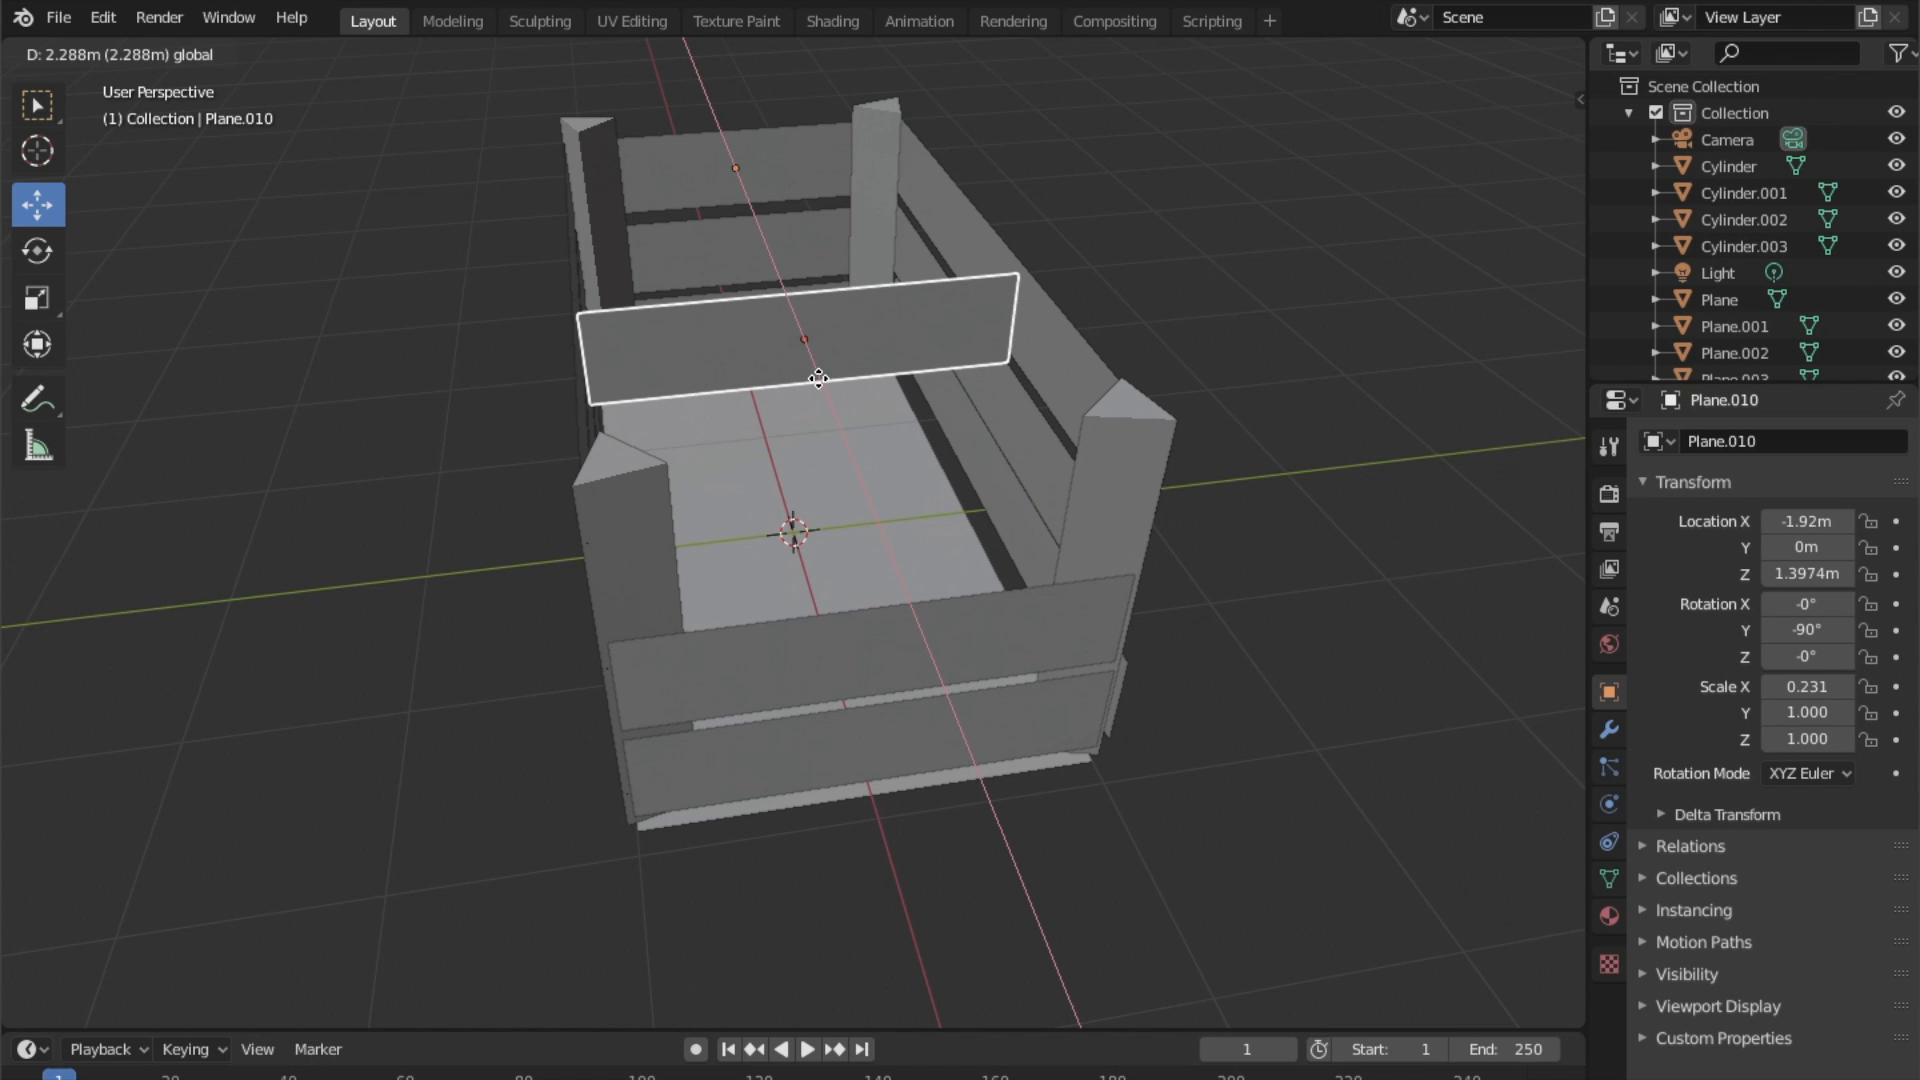
\includegraphics[width=0.75\linewidth]{Figs/VideoBlender06}\\
	    \end{tabular}
    \end{center}	
\end{column}
\begin{column}{0.23\textwidth}
    \begin{center}
	    \begin{tabular}{c}
		        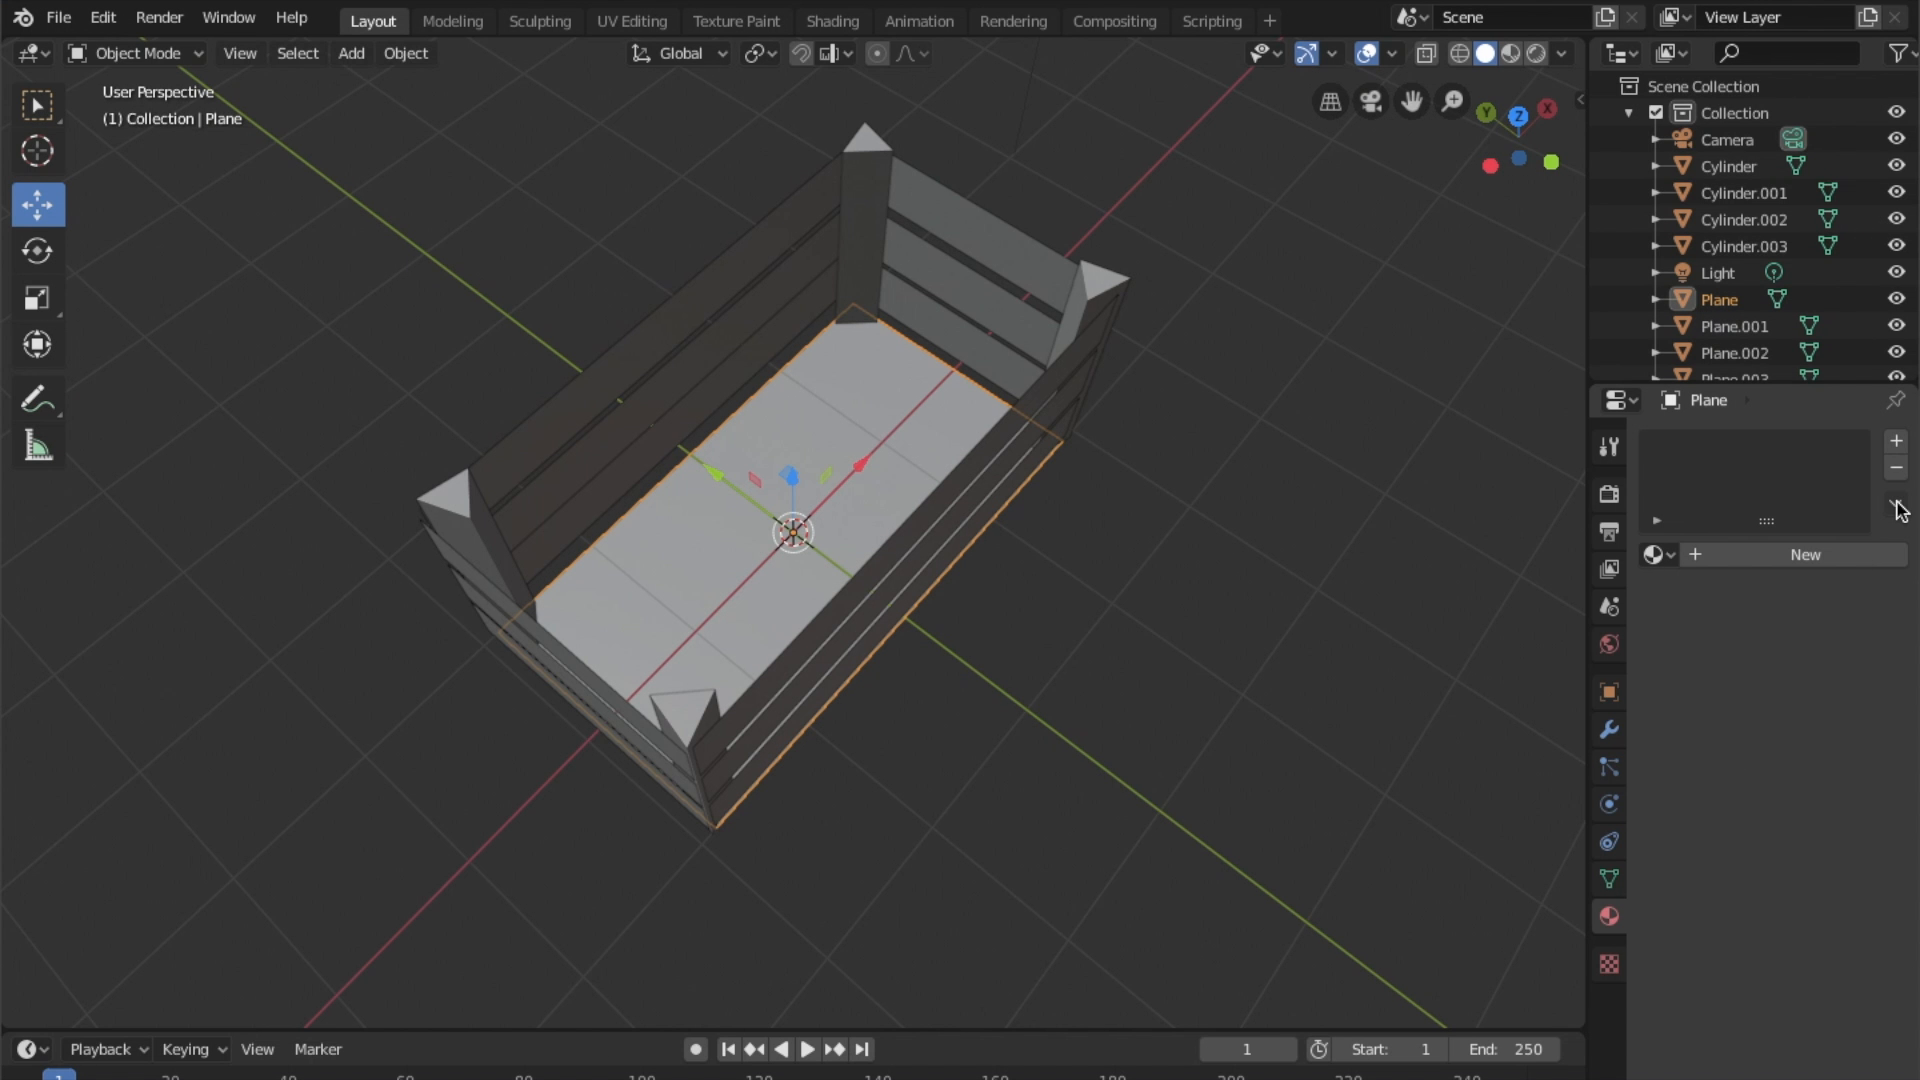
\includegraphics[width=0.75\linewidth]{Figs/VideoBlender07}\\
		        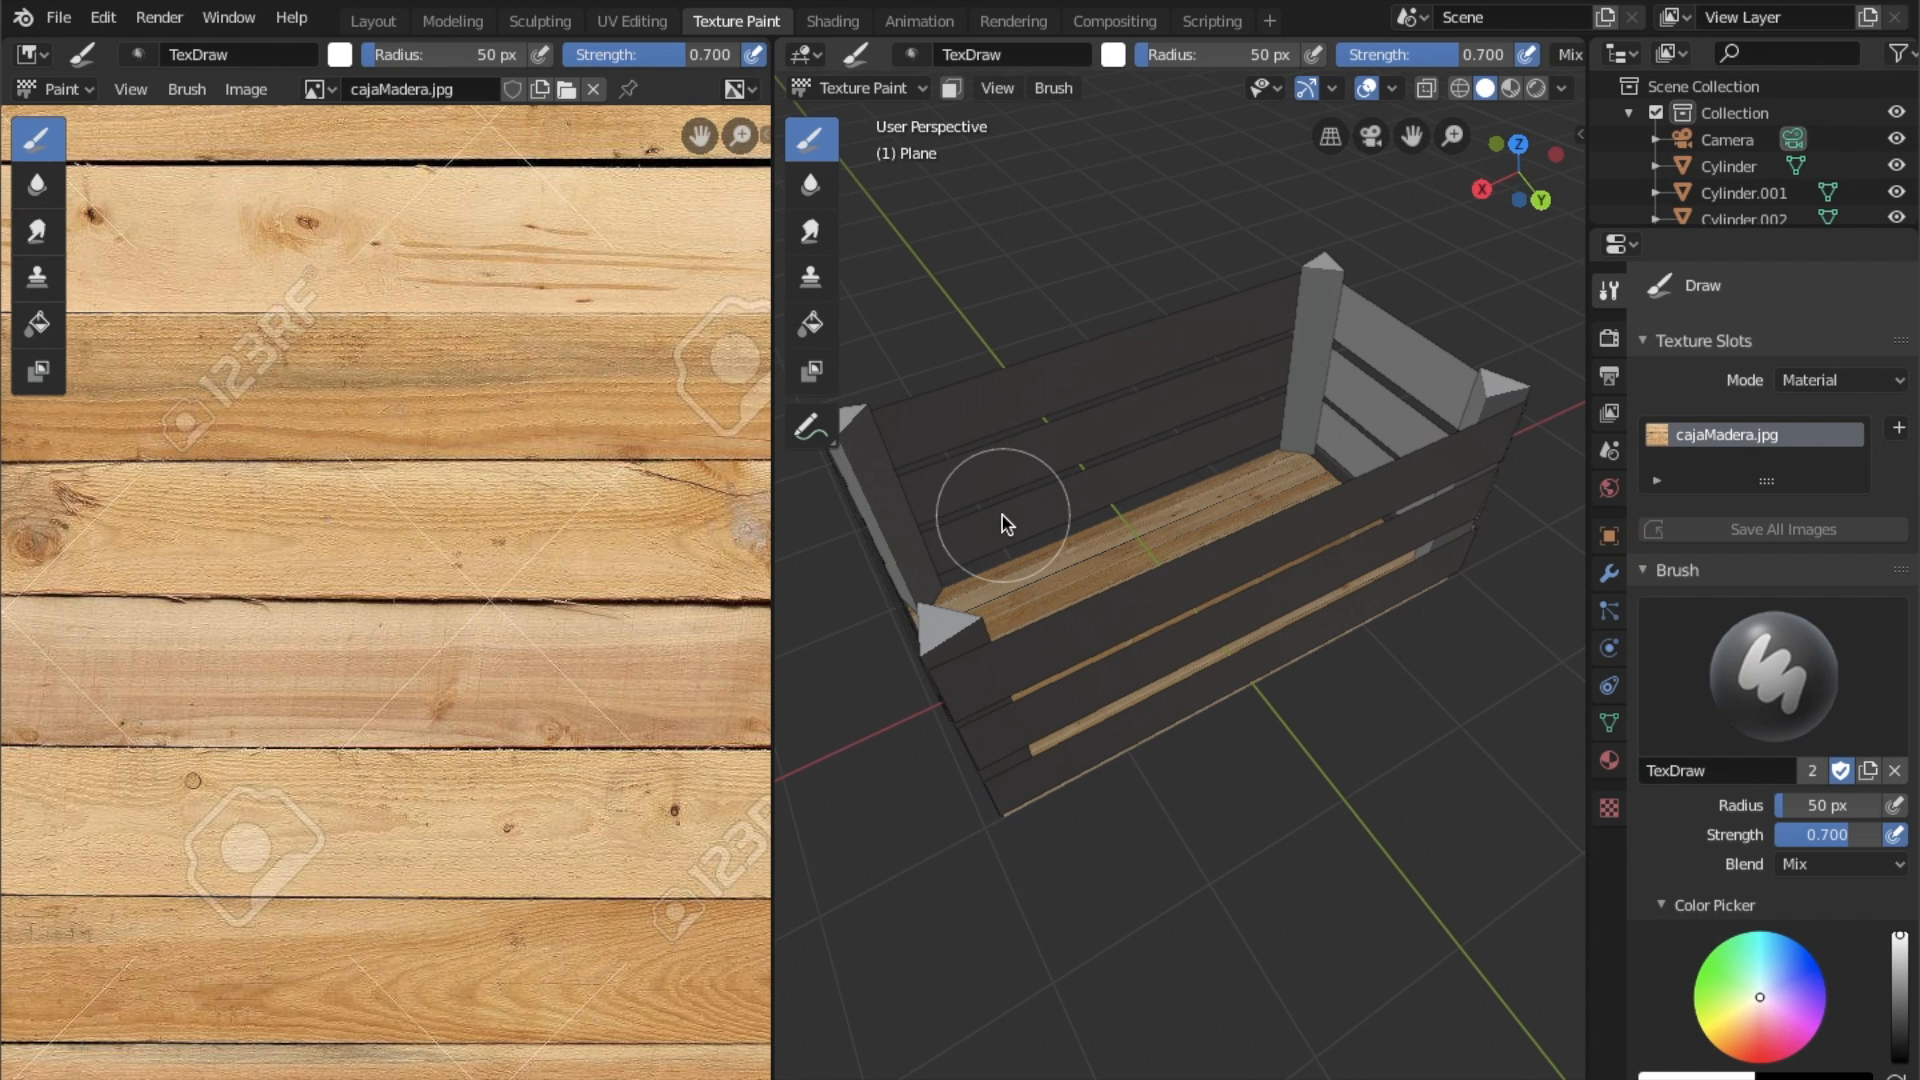
\includegraphics[width=0.75\linewidth]{Figs/VideoBlender08}\\
		        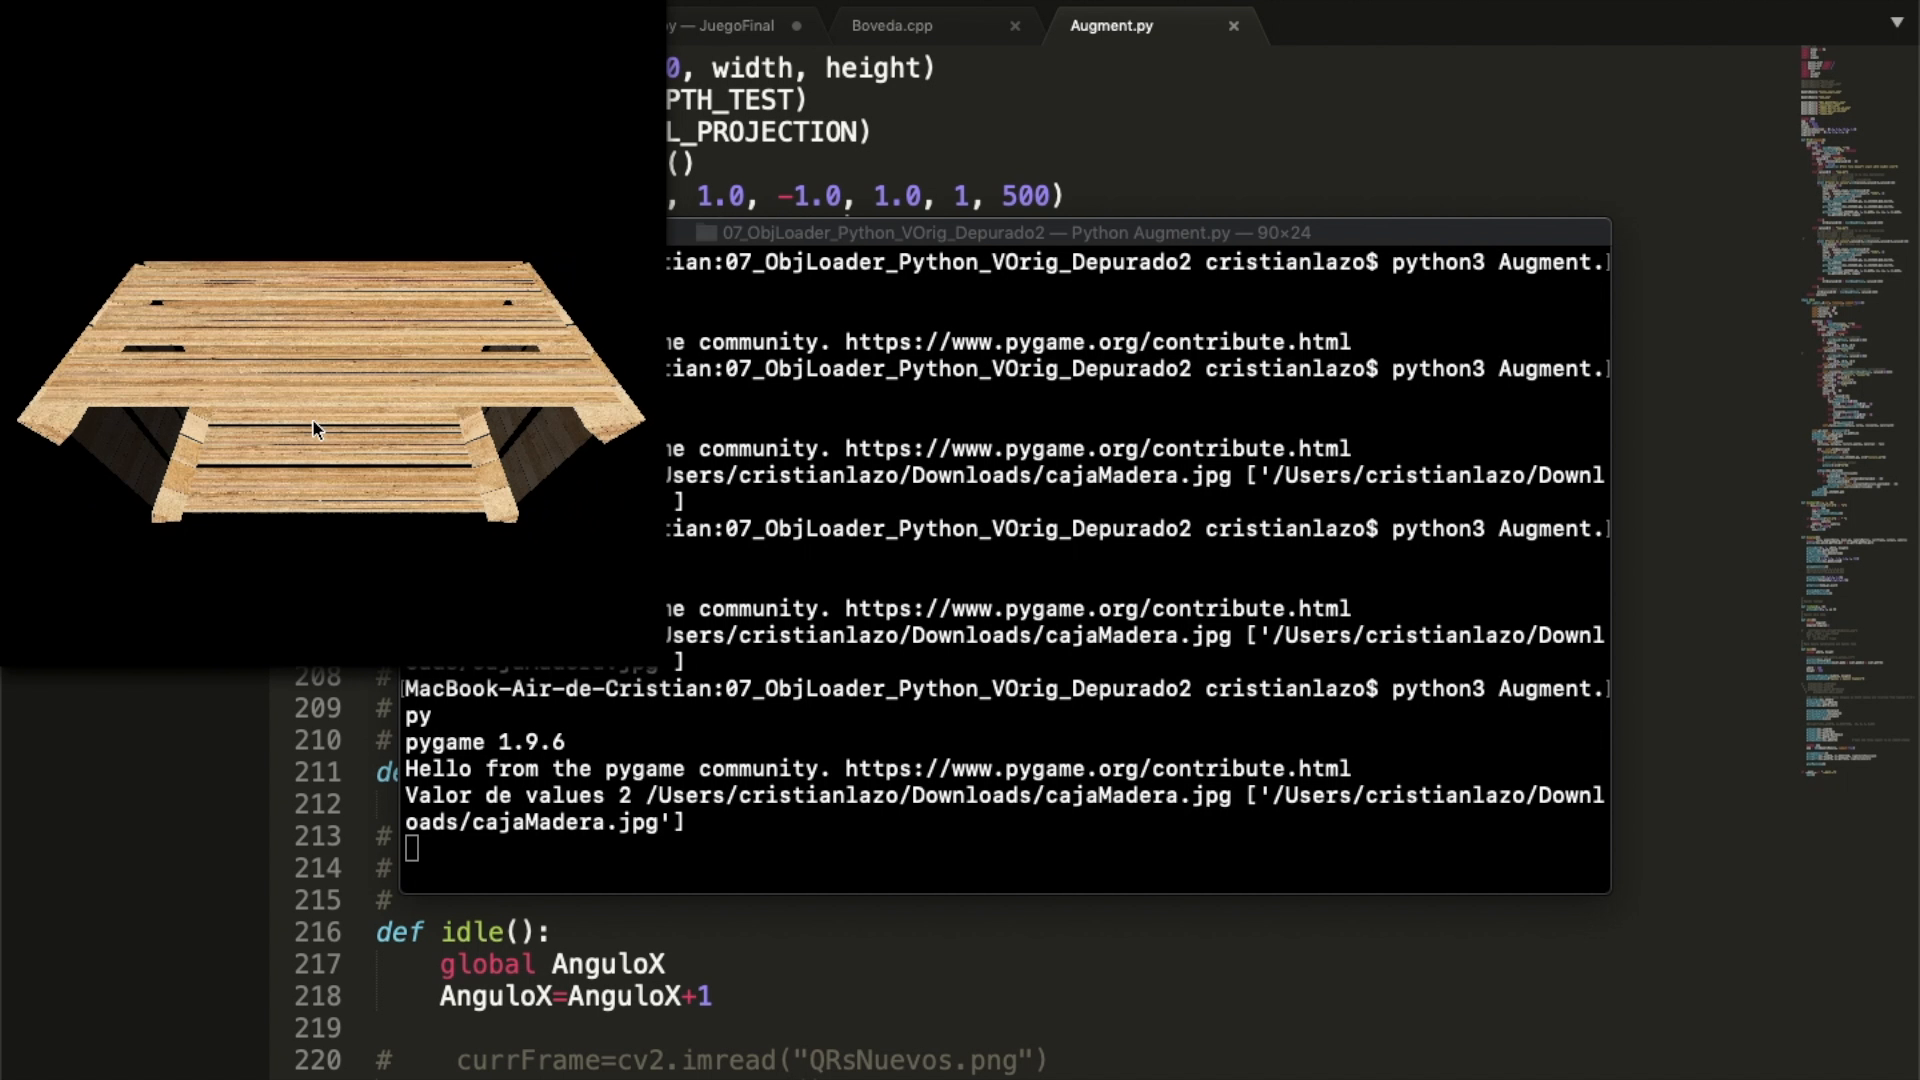
\includegraphics[width=0.75\linewidth]{Figs/VideoBlender09}\\
	    \end{tabular}
    \end{center}	
\end{column}
\begin{column}{0.23\textwidth}
    \begin{center}
	    \begin{tabular}{c}
		        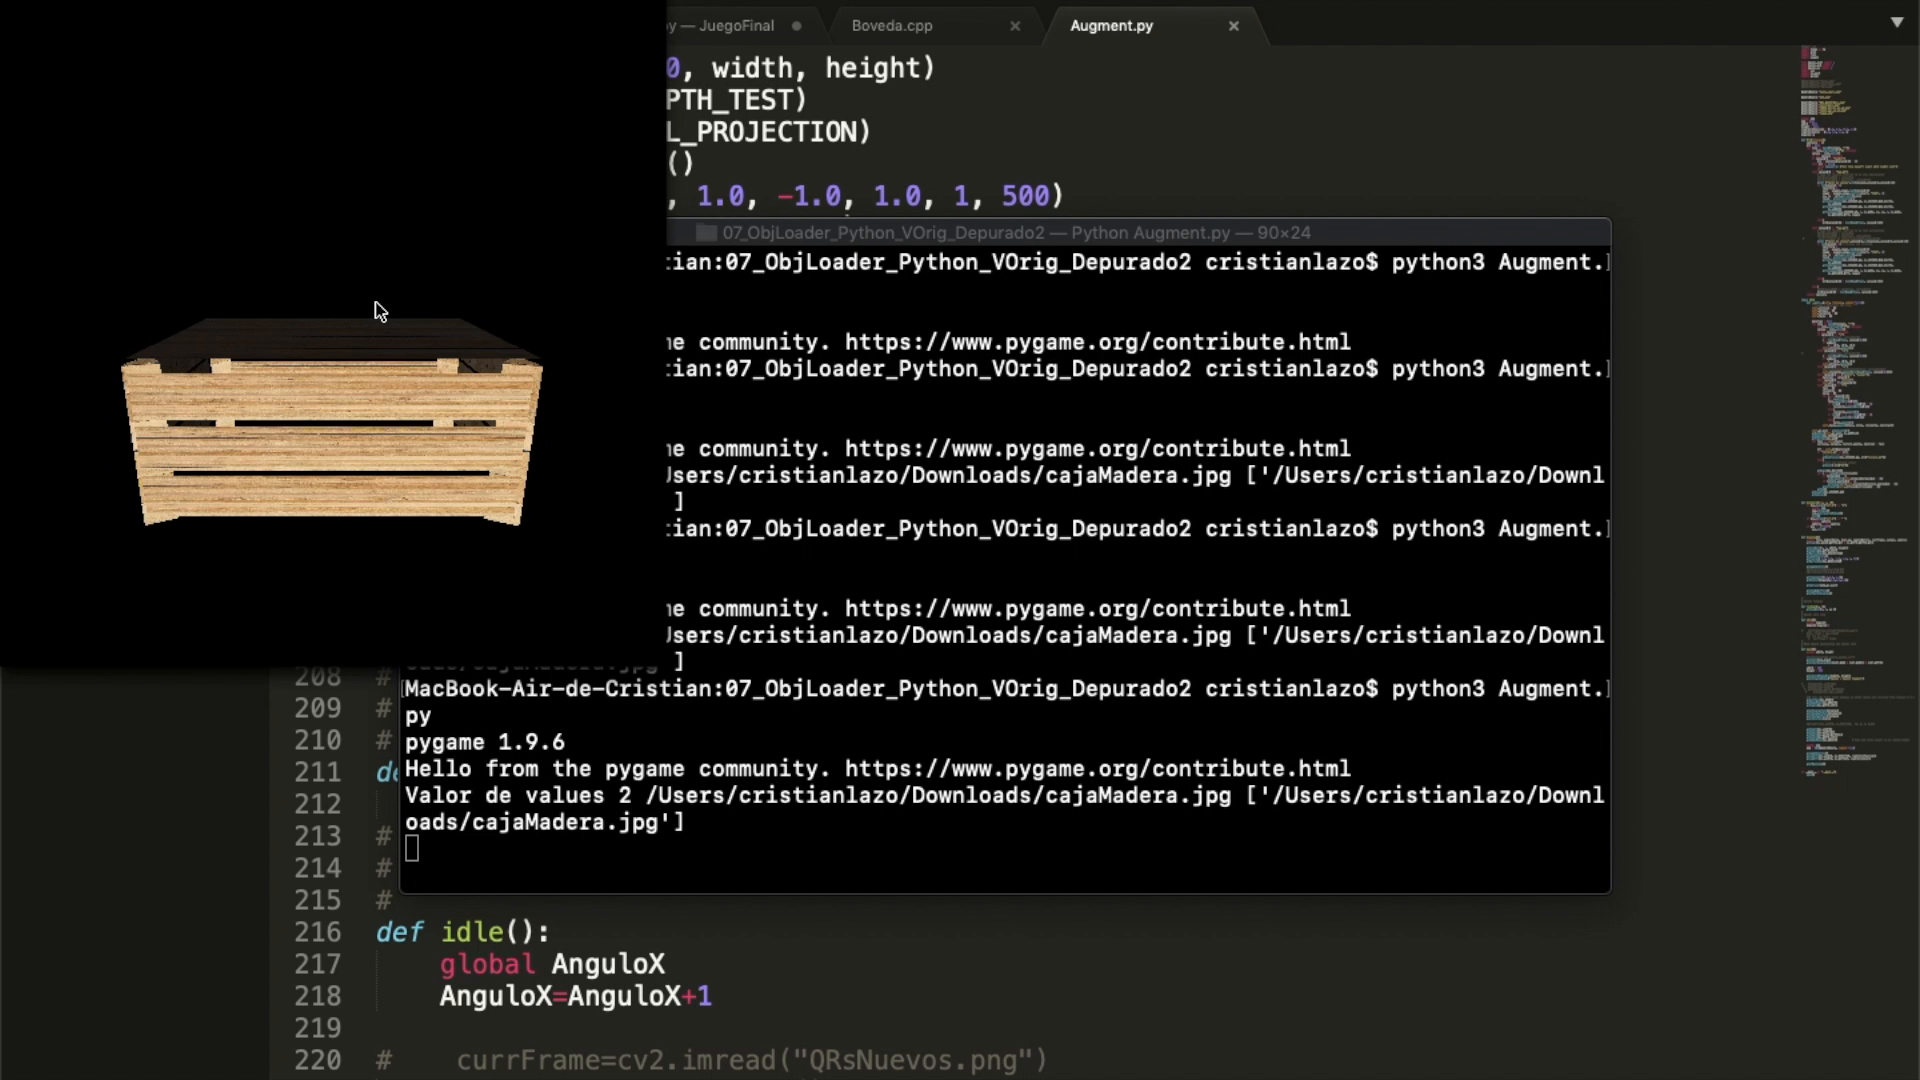
\includegraphics[width=0.75\linewidth]{Figs/VideoBlender10}\\
		        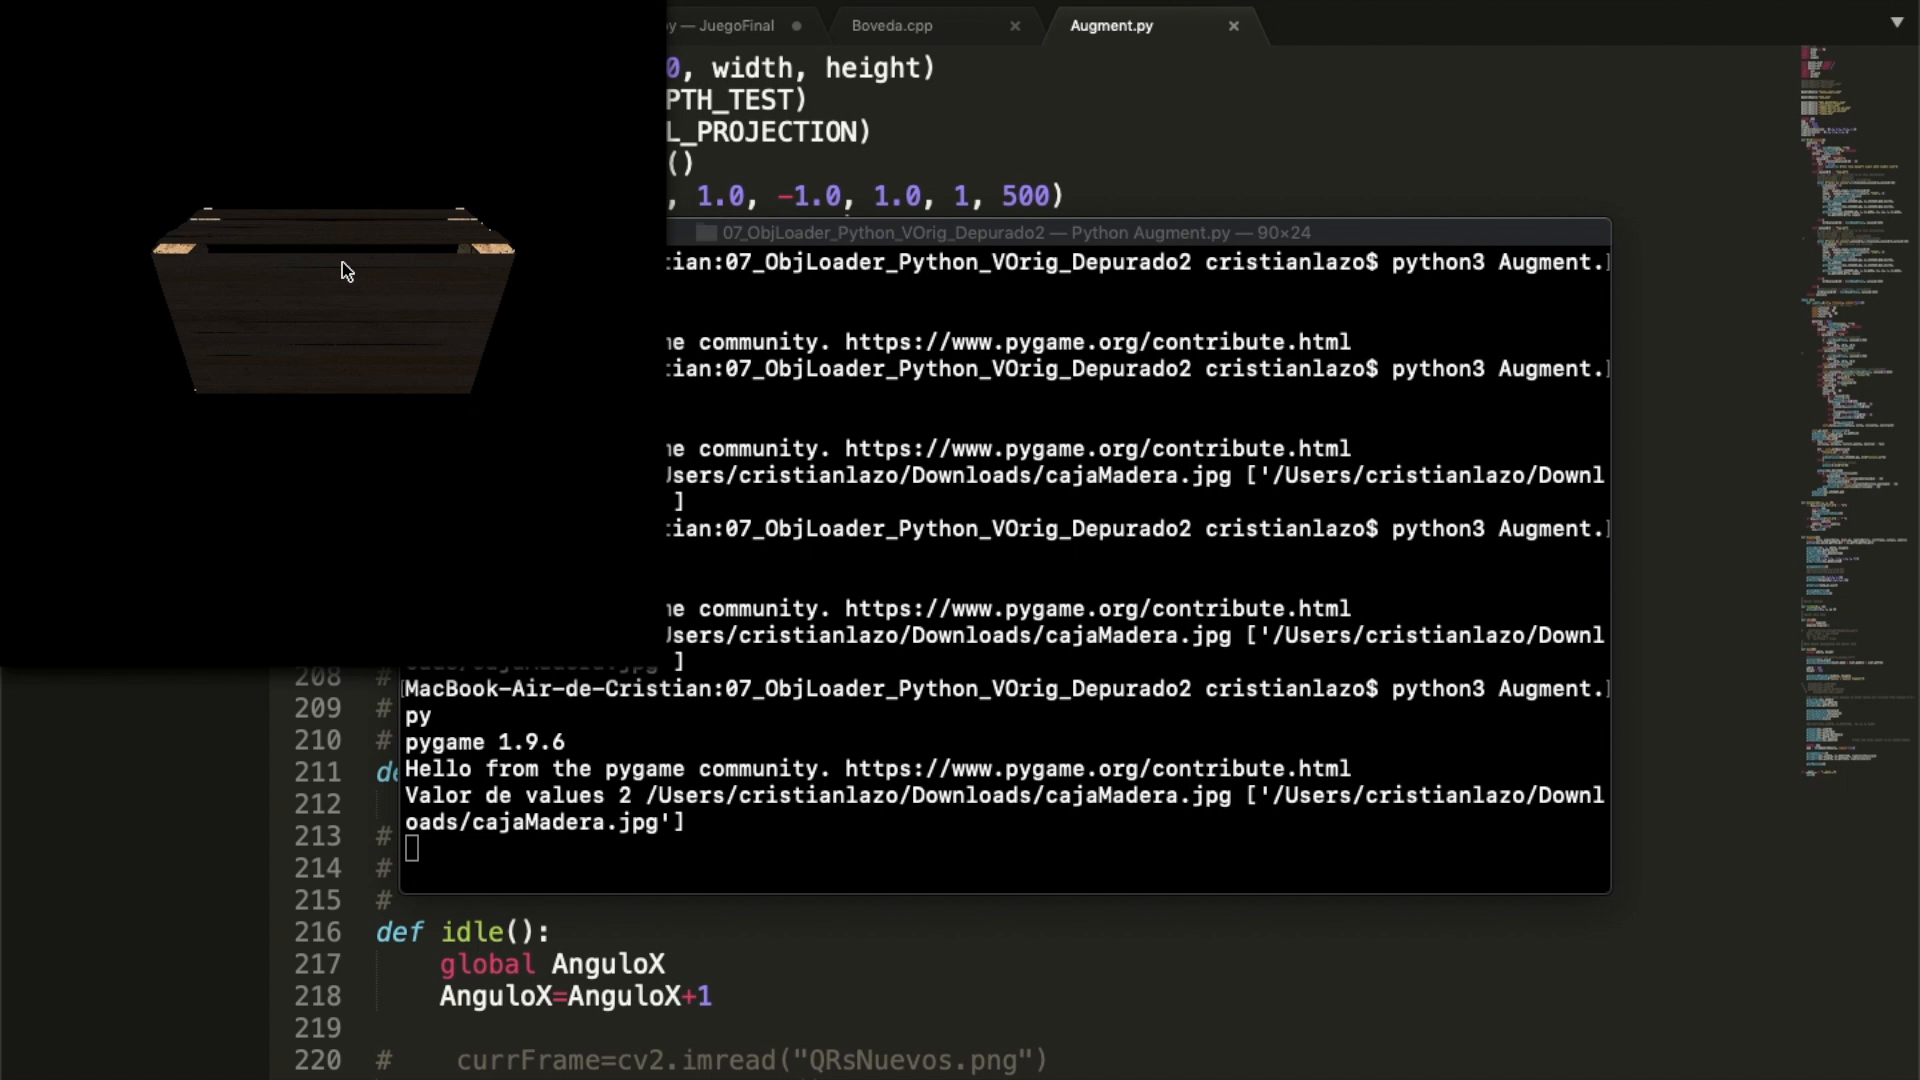
\includegraphics[width=0.75\linewidth]{Figs/VideoBlender11}\\
		        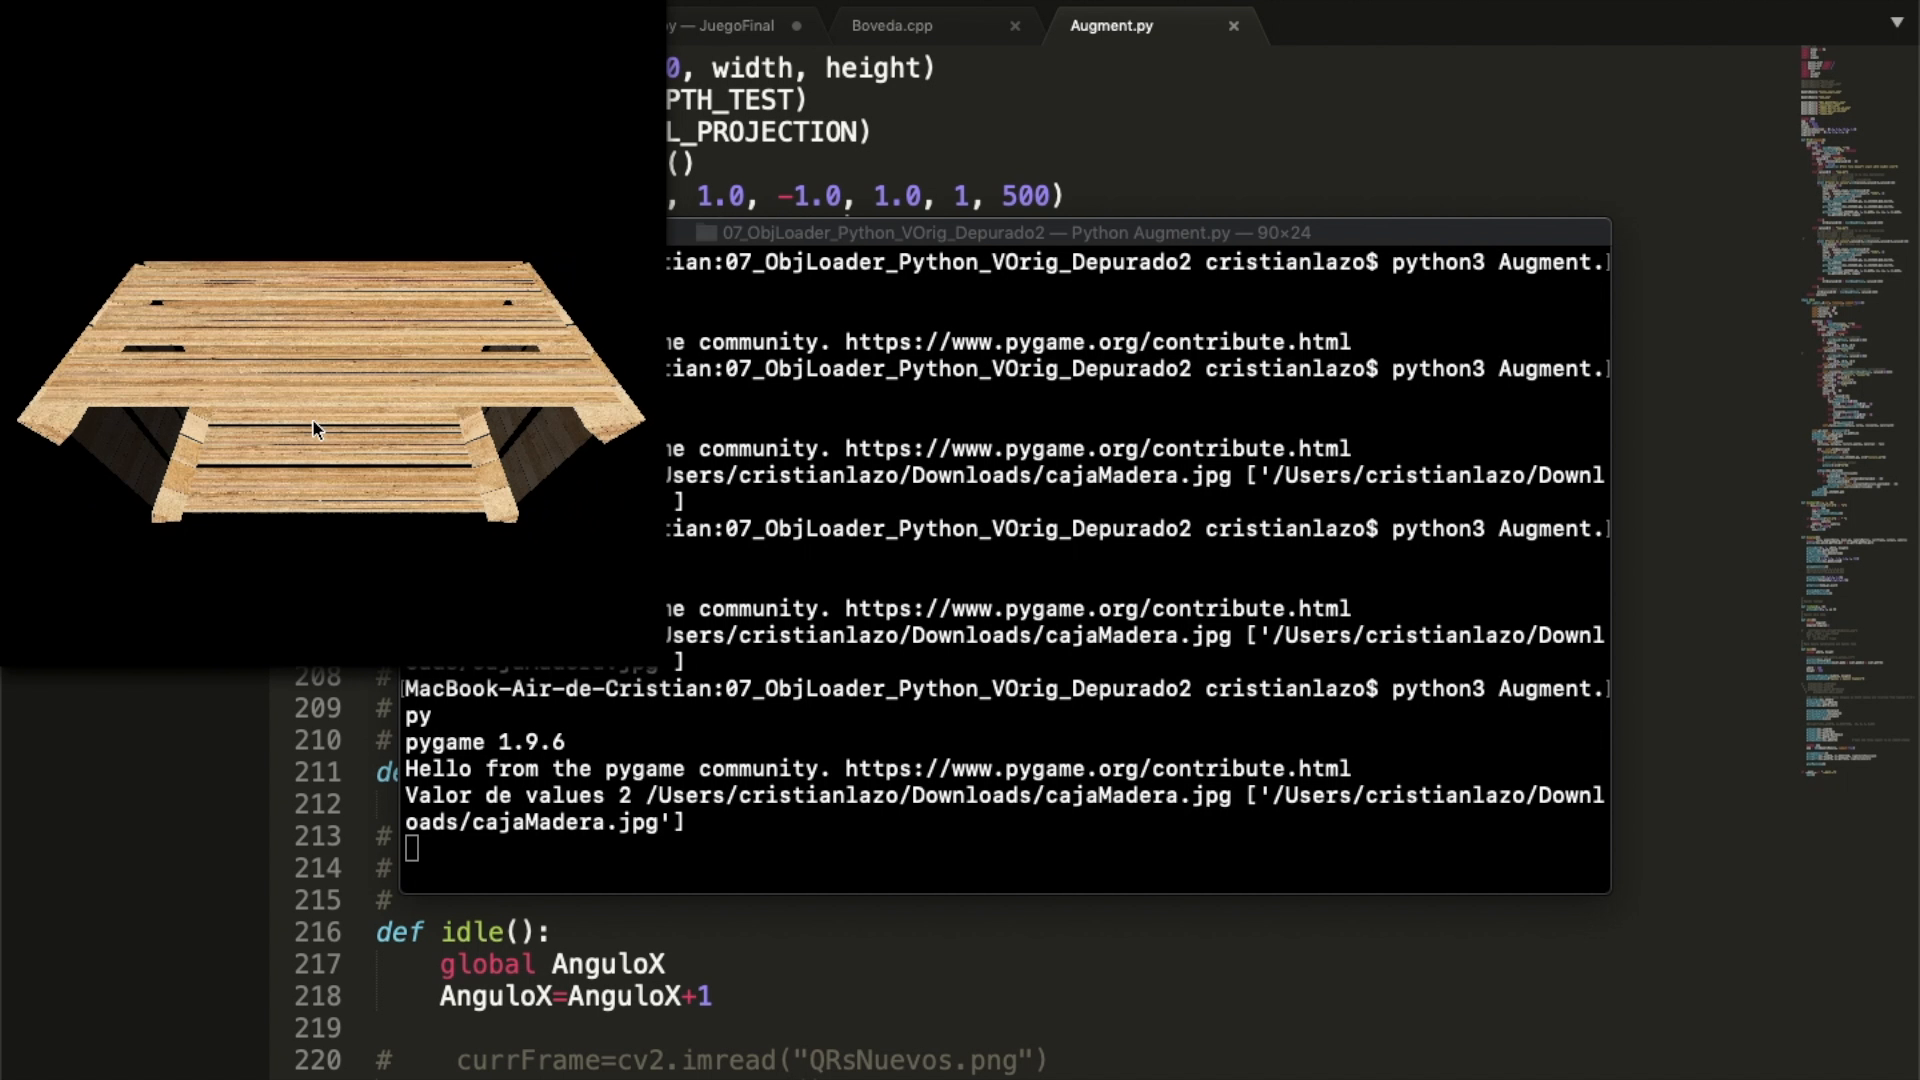
\includegraphics[width=0.75\linewidth]{Figs/VideoBlender12}\\
	    \end{tabular}
    \end{center}	
\end{column}

\end{columns}
%\end{block} 
\footnotetext[1]{\fullcite{\EntradaBibtex}}
\end{frame}


%



%\begin{frame}{\citetitle{MarcoNuno_CongArbEsp_2020_09_01} \footnotemark (1)}

\renewcommand{\EntradaBibtex}{MarcoNuno_CongArbEsp_2020_09_01}
\begin{frame}{\citetitle{\EntradaBibtex} \footnotemark[1] (1)}


\begin{block}{Detección de conductores autorizados \footnotemark } 
\begin{columns}
\begin{column}{1.0\textwidth}
Se propone un sistema montado en un teléfono inteligente que pueda:
	\begin{itemize}
\item Confirmar de manera continua la identidad de los ocupantes empleando la cámara frontal o posterior
\item Monitorear la ubicación del vehículo mediante el sensor GPS
\item Monitorear cuando el vehículo está en movimiento mediante los acelerómetros
\item Trabajar de manera independiente, conectado continuamente a la corriente y con conexión de datos propia para comunicación externa
	\end{itemize}
\end{column}
\end{columns}
\end{block} 
\footnotetext[1]{\fullcite{\EntradaBibtex}}
\end{frame}


\begin{frame}{\citetitle{\EntradaBibtex} (2)}
%\begin{block}{Detección de conductores autorizados (2)} 
\begin{columns}
\begin{column}{0.55\textwidth}
Fases de la ejecución:
	\begin{enumerate}
\item Enrolamiento: Los usuarios usan el automovil y sus rostros quedan guardados.
\item Prueba: Se reporta el ingreso de cualquier extraño.
	\end{enumerate}
Limitaciones:
	\begin{itemize}
\item Solo piloto, copiloto y tal vez pasajero viajando en el centro de la parte posterior.
\item Iluminación diurna.
\item Camuflaje en fase temprana.
	\end{itemize}

\end{column}
\begin{column}{0.45\textwidth}
\begin{center}
     %%%%% this is a minipage, so \textwidth is already adjusted to the size of the column
     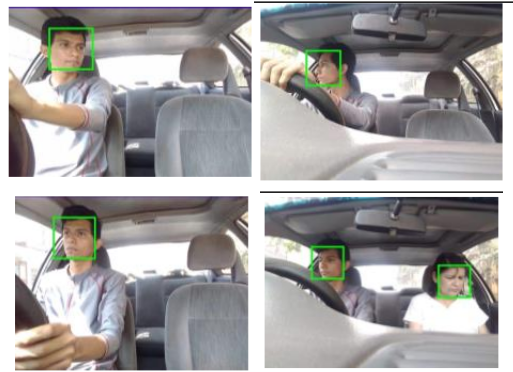
\includegraphics[width=0.99\textwidth]{Figs/ConductorAutorizado1}
     \end{center}
\end{column}

\end{columns}
%\end{block} 
\end{frame}



%
%\begin{frame}{\citetitle{MarcoNuno_Revista_2020_06_00} \footnotemark (1)}

\renewcommand{\EntradaBibtex}{MarcoNuno_Revista_2020_06_00}
\begin{frame}{\citetitle{\EntradaBibtex} \footnotemark[1] (1)}

\begin{block}{Sistema de Monitoreo de Aprendizaje Remoto } 

Con la reciente pandemia, se detectan problemas con el seguimiento del aprendizaje:

	\begin{itemize}
		\item No es posible determinar si el estudiante es quien realiza las tareas
		\item No hay certeza de que tanto tiempo el estudiante dedica a ciertas tareas
	\end{itemize}

Se propone una herramienta cuyos componentes son:
\begin{itemize}
\item Aplicación de Escritorio - El docente asigna tareas·
\item Aplicación en la NUBE - Almacena tareas y evidencias (fotos).
\item Aplicación de Móvil - Monitorea al estudiante emplenado la cámara frontal del teléfono inteligente, además le permite recopilar evidencias.
\end{itemize}
\end{block} 
\footnotetext[1]{\fullcite{\EntradaBibtex}}
\end{frame}

\begin{frame}{\citetitle{\EntradaBibtex}  (2)}


\begin{columns}
\begin{column}{0.65\textwidth}
\begin{block}{La aplicación de escritorio:} 
		\begin{itemize}
		\item Permite crear grupos, tareas, dar de alta alumnos
		\item Descargar evidencias
		\item Generar una gráfica de tiempo de atención
		\end{itemize}
\end{block} 
\begin{block}{La aplicación móvil:} 
		\begin{itemize}
		\item Recibe las tareas y las muestra al alumno
		\item Monitorea al estudiante a lo largo del desarrollo de sus tareas
		\end{itemize}
\end{block} 
\end{column}
\begin{column}{0.35\textwidth}  
    \begin{center}
     %%%%% this is a minipage, so \textwidth is already adjusted to the size of the column
     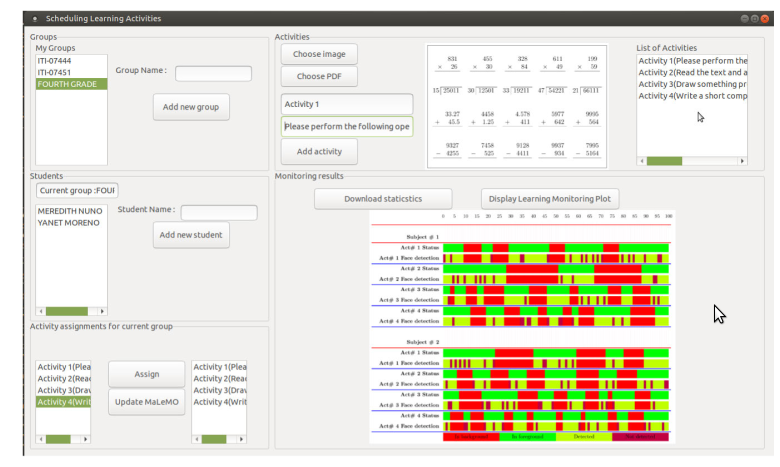
\includegraphics[width=0.95\textwidth]{Figs/LearningMonitoring1}
     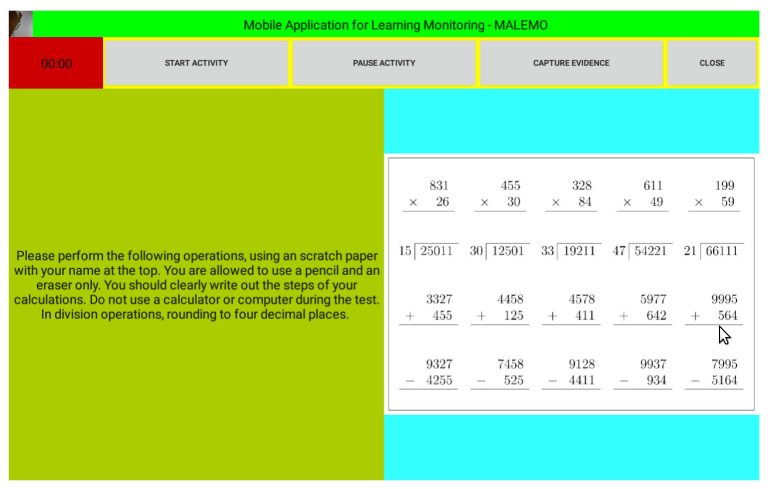
\includegraphics[width=0.95\textwidth]{Figs/LearningMonitoring2}
     \end{center}
\end{column}
\end{columns}


\end{frame}

%\begin{frame}{\citetitle{MarcoNuno_Revista_2020_06_00} (3)}
\begin{frame}{\citetitle{\EntradaBibtex}  (3)}

\begin{columns}
\begin{column}{0.5\textwidth}
\begin{block}{Pasos ejecutados por la App: } 
		\begin{itemize}
		\item Detecta la cara del estudiante y estima hacia donde esta mirando (la pantalla, el área de trabajo o el exterior)
		\item Detecta cuando el estudiante cierra la aplicación y lleva la cuenta del tiempo que la aplicación de monitoreo permanece inactiva. 
		\end{itemize}
\end{block} 
	\begin{center}
		 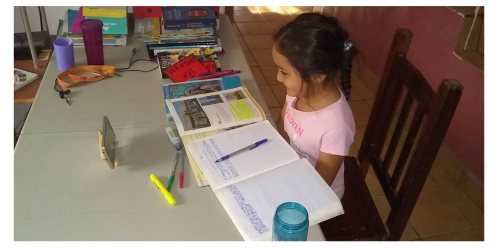
\includegraphics[width=0.50\textwidth]{Figs/LearningMonitoring3}
	\end{center}
\end{column}
\begin{column}{0.5\textwidth}  
    \begin{center}
     %%%%% this is a minipage, so \textwidth is already adjusted to the size of the column
     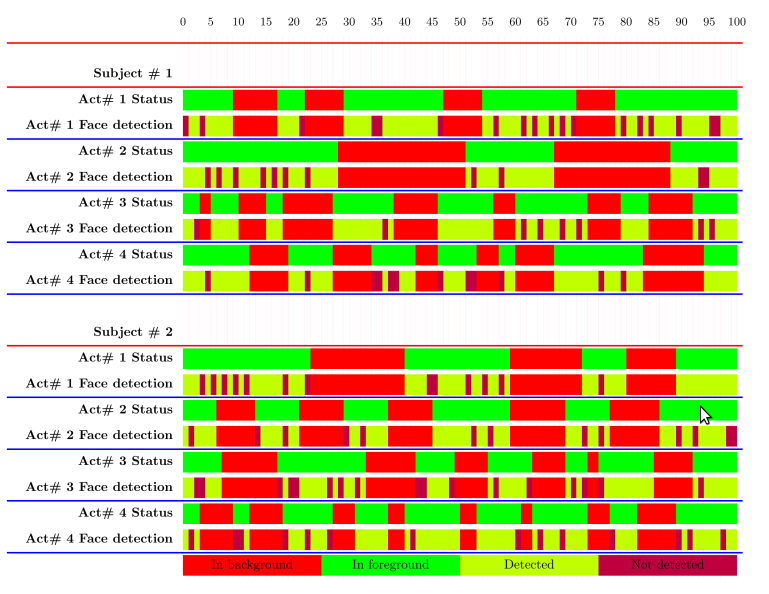
\includegraphics[width=0.99\textwidth]{Figs/LearningMonitoring4}
     \end{center}
\end{column}
\end{columns}

%\end{block} 
\end{frame}



%\renewcommand{\EntradaBibtex}{JaguarAplicacionMovil_2020}
\begin{frame}{\citetitle{\EntradaBibtex} \footnotemark[1] (1)}


%\begin{frame}{Desarrollos Tecnológicos}
\begin{block}{-} 
\begin{columns}
\begin{column}{0.48\textwidth}
		\begin{itemize}
		\item Detección de Codigos QR
		\item Modelado de la mascota en 3D mediante el Software Blender
		\item Sobreposición del modelo 3D dependiendo de la posición del código QR
		\end{itemize}
	\end{column}
	\begin{column}{0.52\textwidth}  
	    \begin{center}
	    	 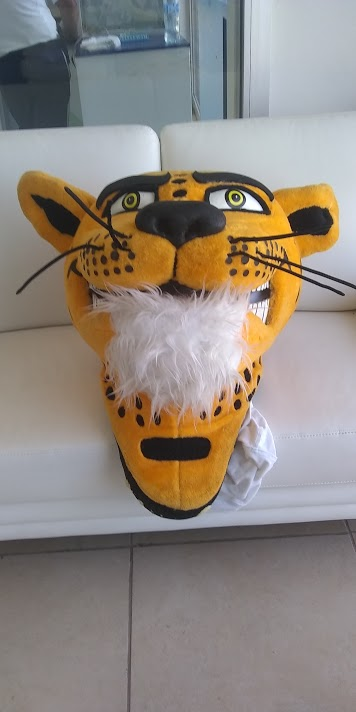
\includegraphics[width=0.25\textwidth]{Figs/JaguarFisico01}
	    	 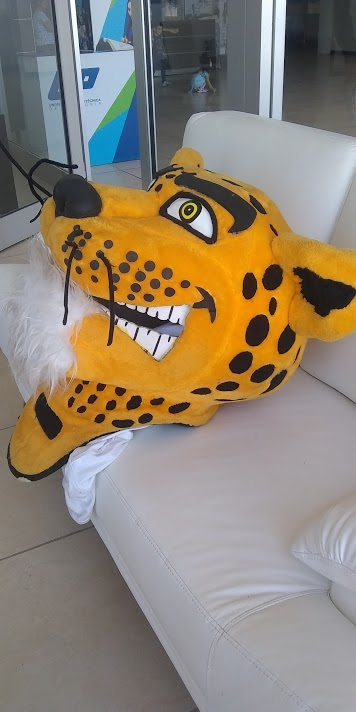
\includegraphics[width=0.25\textwidth]{Figs/JaguarFisico02}\\
    	 \end{center}
	\end{column}
	\end{columns}
	\end{block} 
	%\footnotetext{\fullcite{JaguarAplicacionMovil_2020}}
\footnotetext[1]{\fullcite{\EntradaBibtex}}
%\footnotetext{Andrés García González, Cristian Aléxis Lazo García, Damaris Mendoza Vázquez.  \textbf{Modelo 3D del Jaguar de la UPV sobre un código QR}. Universidad Politécnica de Victoria,  Informe técnico proyecto de asignatura ``Graficación por Computadora Aavanzada'', 2020. Sin Publicar.}
%\\setcounter{footnote}{0}
\end{frame}


\begin{frame}{\citetitle{\EntradaBibtex} (2)}
\begin{block}{-} 
\begin{columns}
	\begin{column}{0.98\textwidth}
	    \begin{center}
	    	 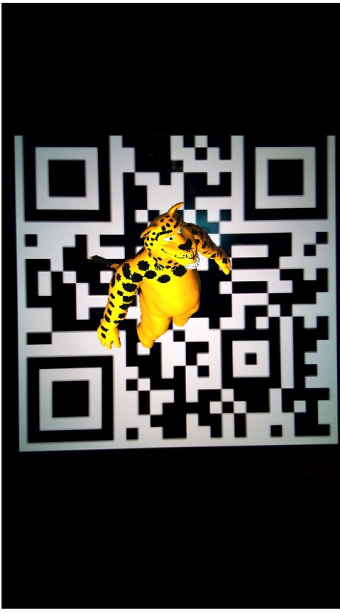
\includegraphics[width=0.24\textwidth]{Figs/JaguarVirtual01}
	    	 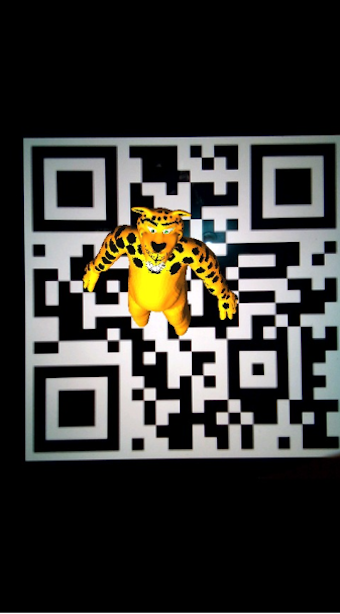
\includegraphics[width=0.24\textwidth]{Figs/JaguarVirtual02}
	    	 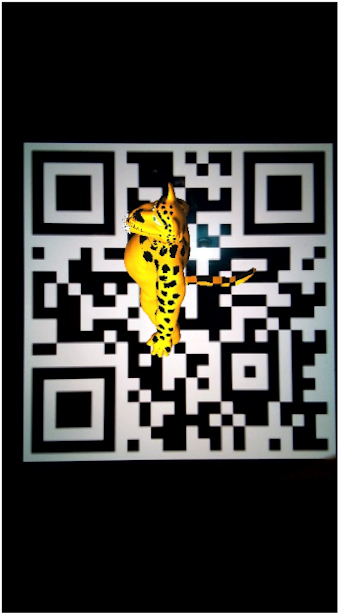
\includegraphics[width=0.24\textwidth]{Figs/JaguarVirtual03}
	    	 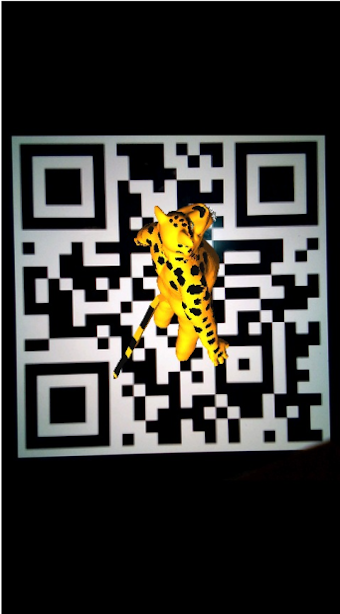
\includegraphics[width=0.24\textwidth]{Figs/JaguarVirtual04}
    	 \end{center}
	\end{column}
	\end{columns}
	\end{block} 
\end{frame}


%
\renewcommand{\EntradaBibtex}{MarcoNuno_Revista_2020_04_00}
\begin{frame}{\citetitle{\EntradaBibtex} \footnotemark[1] (1)}



%\begin{frame}{Proyectos de Investigación}

\begin{columns}
\begin{column}{0.70\textwidth}
Propuesta:
		\begin{itemize}
		\item Un \textit{Cariograma} es una representación ordenada de los cromosomas.  
		\item Un \textit{Citogenetista} es una experto que diagnotisca enfermedades genéticas a partir de Cariograma.		
		\item Un sistema que auxilie al Citogenetista a crear el Cariograma de forma automática.
		\item Se requieren técnicas de visión por computadora y aprendizaje automáticos.
		\end{itemize}
\end{column}
\begin{column}{0.30\textwidth}  
    \begin{center}
     %%%%% this is a minipage, so \textwidth is already adjusted to the size of the column
     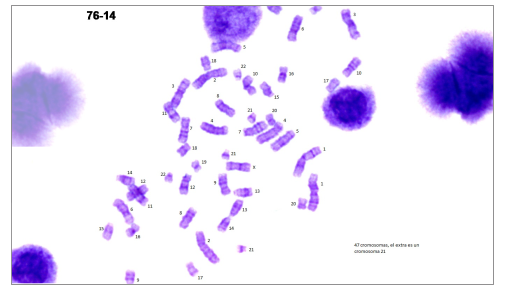
\includegraphics[width=0.98\textwidth]{Figs/Karyogram1}
     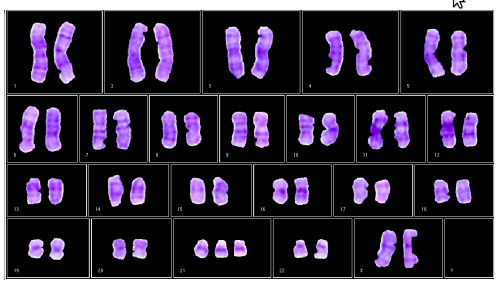
\includegraphics[width=0.98\textwidth]{Figs/Karyogram2}
     \end{center}
\end{column}
\end{columns}
\footnotetext[1]{\fullcite{\EntradaBibtex}}
\end{frame}


\begin{frame}{\citetitle{\EntradaBibtex} (2)}
\begin{columns}
\begin{column}{0.6\textwidth}
Pasos a aplicar:
		\begin{enumerate}
		\item Segmentación de los cromosomas individuales 
		\item Extracción de características
		\item Clasificación por tamaño
		\item Clasificación por tipo dentro de cada tamaño
		\item Integración
		\item Construcción del Cariograma
		\end{enumerate}
    \begin{center}
     %%%%% this is a minipage, so \textwidth is already adjusted to the size of the column
     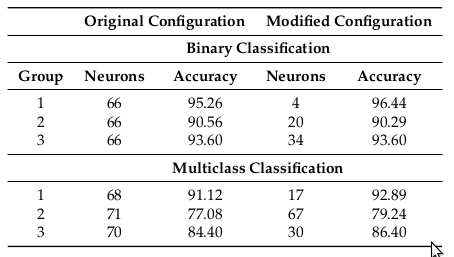
\includegraphics[width=0.5\textwidth]{Figs/Karyogram4}
     \end{center}


\end{column}
\begin{column}{0.4\textwidth}  
    \begin{center}
     %%%%% this is a minipage, so \textwidth is already adjusted to the size of the column
     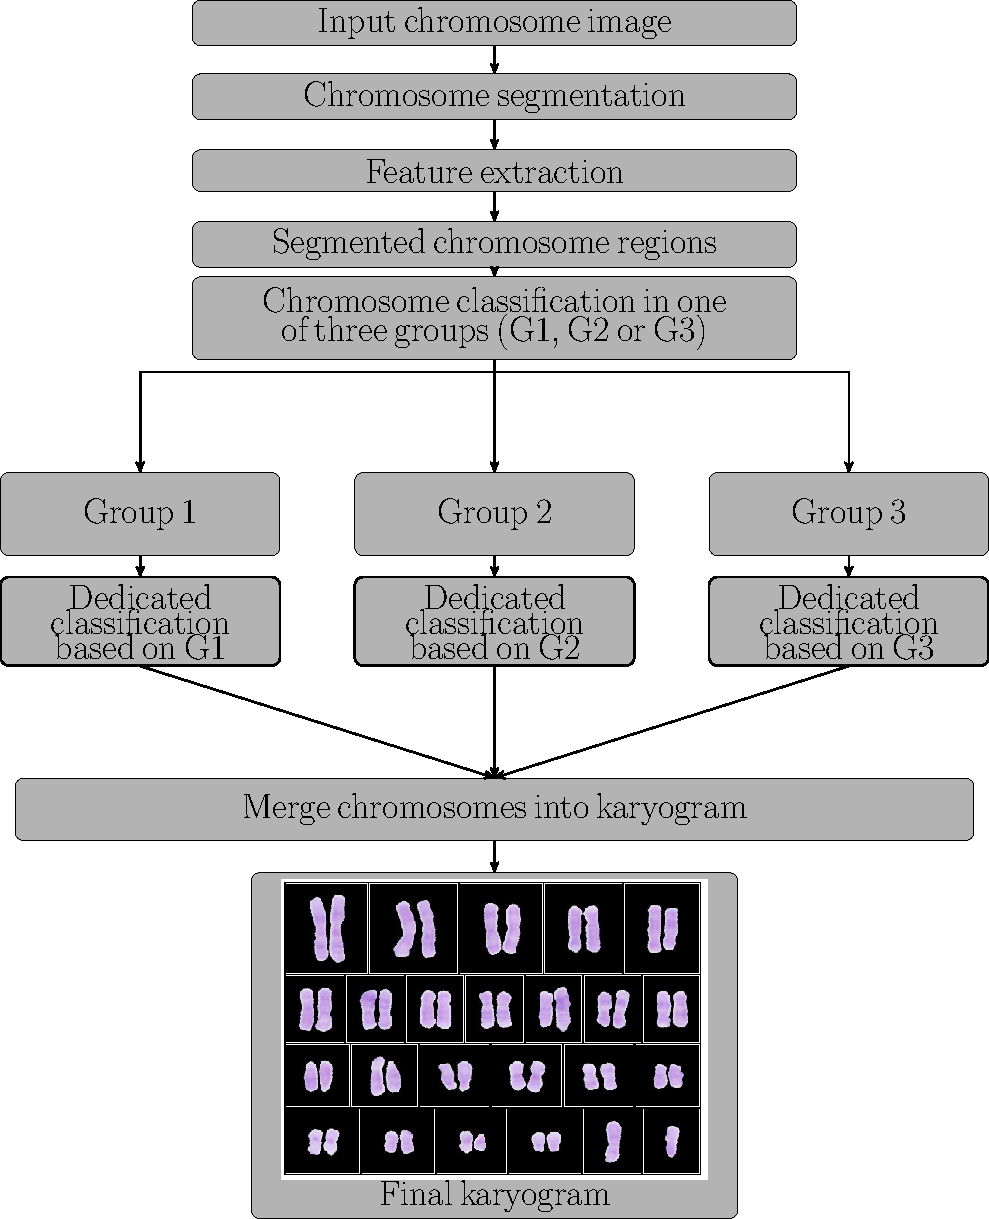
\includegraphics[width=0.7\textwidth]{Figs/Karyogram5}
     \end{center}
\end{column}
\end{columns}
\end{frame}







%

\renewcommand{\EntradaBibtex}{MarcoNuno_CongArbEsp_2019_09_01}
\begin{frame}{\citetitle{\EntradaBibtex} \footnotemark[1] (1)}

%\begin{frame}{\citetitle{MarcoNuno_CongArbEsp_2019_09_01} \footnotemark (1)}
\begin{columns}
\begin{column}{0.6\textwidth}
Los componentes de la báscula inteligente son:
	\begin{itemize}
\item Báscula digital
\item Sensor ultrasónico
\item Cámara
\item Pantalla touch
\item Operada por comandos por voz
\item Controlada por una computadora embebida con conexión a internet (Raspberry-Pi)
	\end{itemize}
\end{column}
\begin{column}{0.4\textwidth}
\begin{center}
     %%%%% this is a minipage, so \textwidth is already adjusted to the size of the column
     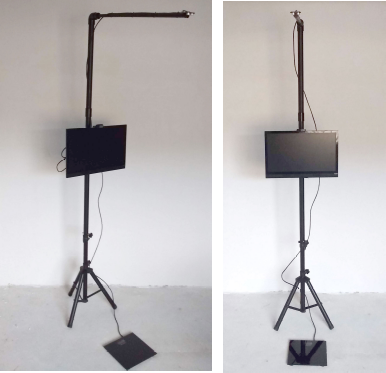
\includegraphics[width=0.99\textwidth]{Figs/Bascula1}
     \end{center}
\end{column}

\end{columns}
\footnotetext[1]{\fullcite{\EntradaBibtex}}
\end{frame}

\begin{frame}{\citetitle{\EntradaBibtex} (2)}
\begin{columns}
\begin{column}{0.35\textwidth}
La interfaz mostrada:
	\begin{itemize}
\item Estima los parámetros obtenidos
\item Estima el Indice de Masa Corporal (IMC)
\item Propone un régimen alimenticio (se recomienda consultar a un especialista)
	\end{itemize}
\end{column}
\begin{column}{0.65\textwidth}
\begin{center}
     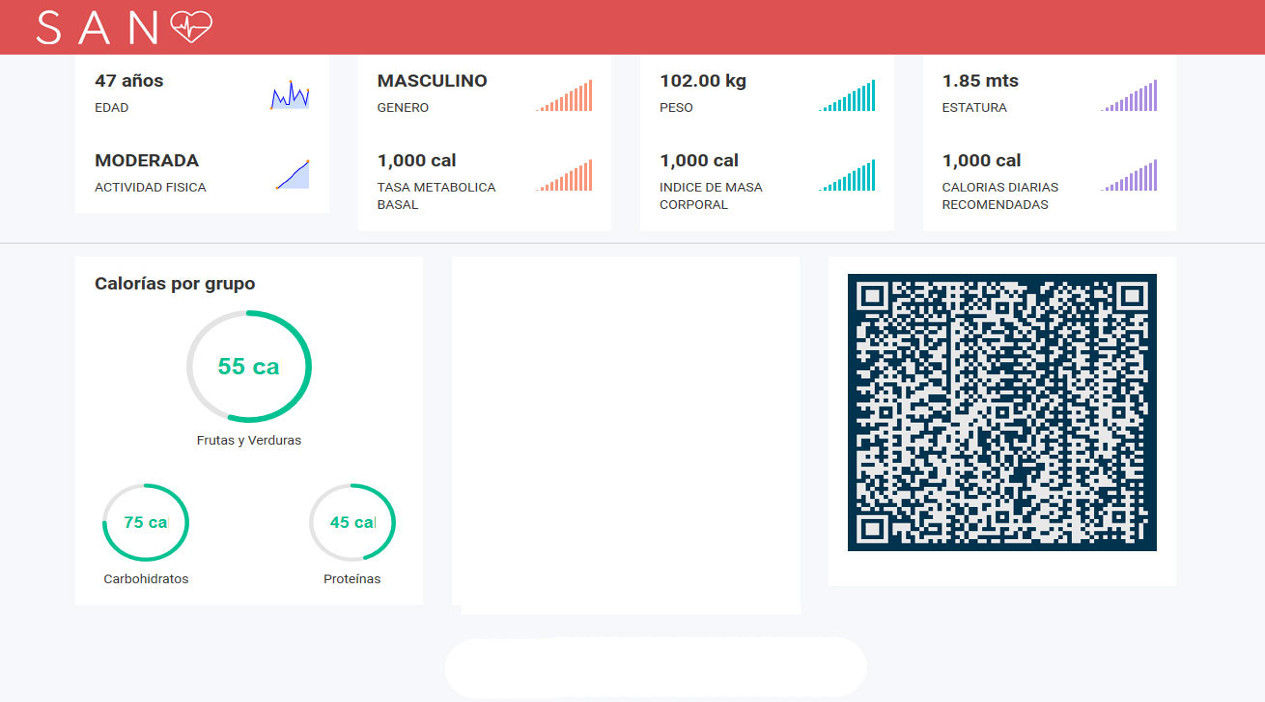
\includegraphics[width=0.99\textwidth]{Figs/Bascula2}
     \end{center}
\end{column}

\end{columns}
\end{frame}




%\renewcommand{\EntradaBibtex}{MarcoNuno_Revista_2020_10_00}
\begin{frame}{\citetitle{\EntradaBibtex} \footnotemark[1] (1)}





\begin{columns}
\begin{column}{0.5\textwidth}
	\begin{itemize}
\item Es necesario herramientas para educar a pacientes con Diabetes para manejar su enfermedad.
\item Se propone una aplicación móvil que permita generar una simulación del comportamiento de la glucosa en un organismo con Diabetes a partir de modelos:
	\begin{itemize}
		\item Dosificación de insulina
		\item Ejercicio
		\item Ingesta de alimentos
	\end{itemize}
	\end{itemize}
\end{column}
\begin{column}{0.5\textwidth}
\begin{center}
     %%%%% this is a minipage, so \textwidth is already adjusted to the size of the column
     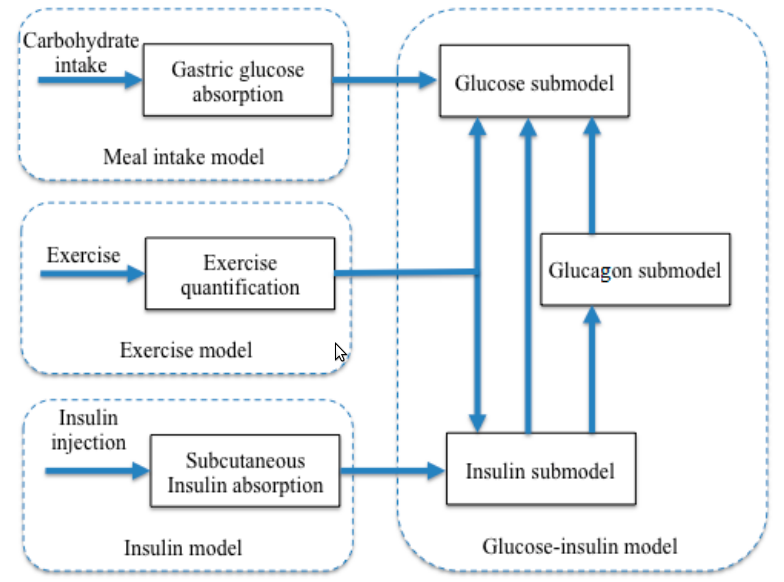
\includegraphics[width=0.99\textwidth]{Figs/Diabetes1}
     \end{center}
\end{column}
\end{columns}
\footnotetext[1]{\fullcite{\EntradaBibtex}}
\end{frame}

\begin{frame}{\citetitle{\EntradaBibtex} (2)}
\begin{columns}
\begin{column}{0.65\textwidth}
Pantallas de la aplicación:
	\begin{enumerate}
\item Pantalla inicial
\item Configuración de ingesta de alimentos
\item Configuración de dosificación de insulina
\item Configuración de configuración de rutina de ejercicio
\item Inicio de simulación
	\end{enumerate}
\end{column}
\begin{column}{0.40\textwidth}
\begin{center}
     %%%%% this is a minipage, so \textwidth is already adjusted to the size of the column
     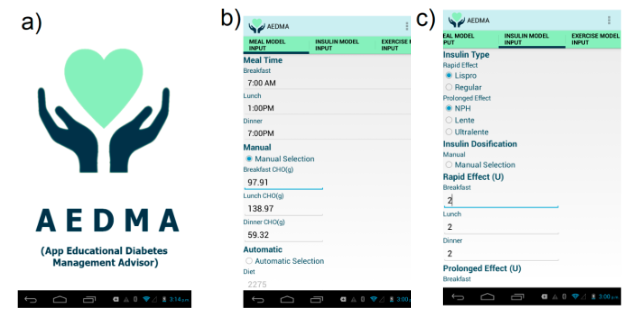
\includegraphics[width=0.99\textwidth]{Figs/Diabetes3}
     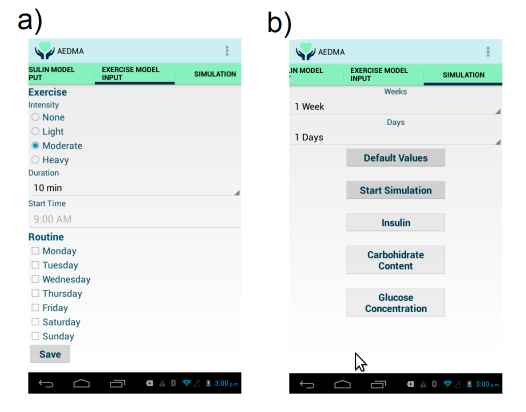
\includegraphics[width=0.66\textwidth]{Figs/Diabetes4}
     \end{center}
\end{column}
\end{columns}
\end{frame}

\begin{frame}{\citetitle{\EntradaBibtex} (3)}
\begin{columns}
\begin{column}{0.65\textwidth}
La aplicación genera una gráfica de comportamiento de la glucosa a lo largo del tiempo de simulación. Se muestran las gráficas para cuatro casos:
	\begin{itemize}
\item Pacientes controlados en cuanto a los niveles de glucosa (a y b)
\item Pacientes fuera de control debido a la falta de ejercicio y al exceso de carbohidratos (c y d)
	\end{itemize}
\end{column}
\begin{column}{0.35\textwidth}
\begin{center}
     %%%%% this is a minipage, so \textwidth is already adjusted to the size of the column
     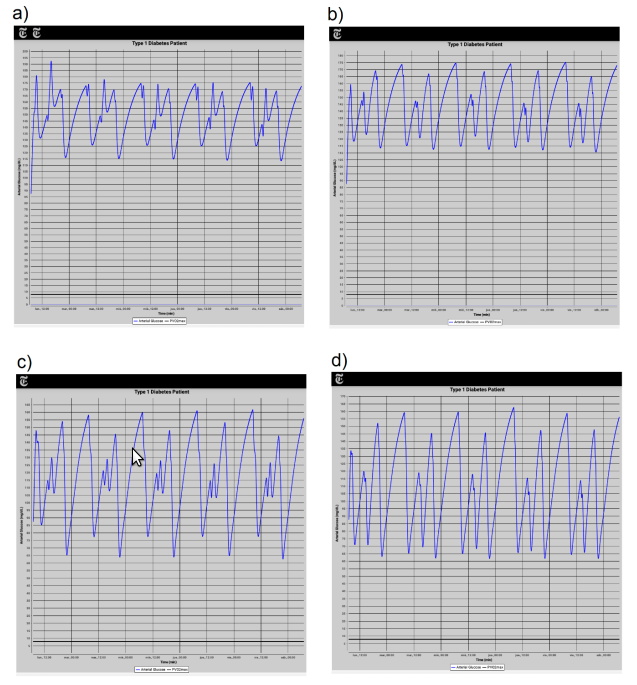
\includegraphics[width=0.99\textwidth]{Figs/Diabetes5}
     \end{center}
\end{column}
\end{columns}
\end{frame}




%
\renewcommand{\EntradaBibtex}{RealidadAumentada_PrimerPrototipo_2019}
\begin{frame}{\citetitle{\EntradaBibtex} \footnotemark[1] (1)}

%\begin{frame}{Sistema de Realidad Aumentada \footnotemark}
%\begin{block}{Sistema de Realidad Aumentada \footnotemark} 
\begin{columns}
\begin{column}{0.48\textwidth}
		\begin{itemize}
		\item Detección de Codigos QR
		\item Decodificación del texto codificado en el codigo QR
		\item Sobreposición del modelo 3D dependiendo de la posición del código QR
		\end{itemize}
	\end{column}
	\begin{column}{0.52\textwidth}  
	    \begin{center}
	    	 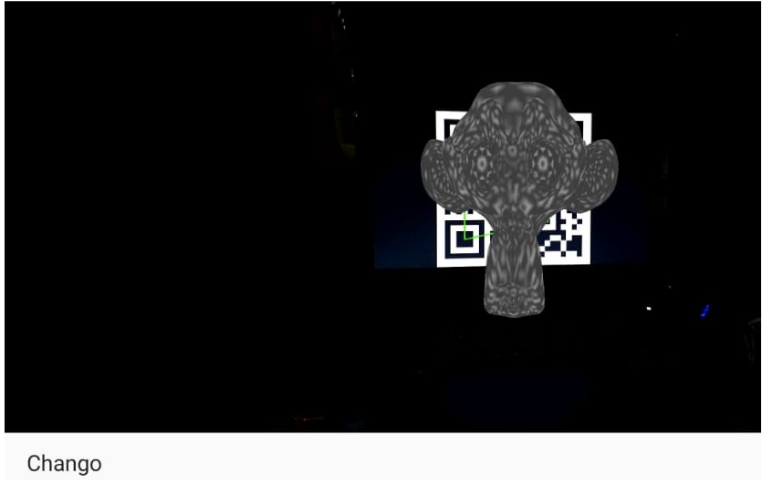
\includegraphics[width=0.95\textwidth]{Figs/SistemaAR1}
    	 \end{center}
	\end{column}
	\end{columns}
%	\end{block} 
\footnotetext[1]{\fullcite{\EntradaBibtex}}
%\footnotetext{Cárdenas Castillo Jesús Alfredo, Molina Pastrana Ana Karen, Ramos Lucio Eluis Carlo, Rodríguez Terán Linda Margarita y Vázquez Luna César Jovany.  \textbf{Visión por Computadora para Realidad Aumentada}. Universidad Politécnica de Victoria,  Informe técnico proyecto de asignatura ``Cómputo en Dispositivos Móviles'', 2019. Sin Publicar.}
%\\setcounter{footnote}{0}
\end{frame}

%Cárdenas Castillo Jesús Alfredo, Molina Pastrana Ana Karen, Ramos Lucio Eluis Carlo, Rodrı́guez Terán Linda Margarita, Vázquez Luna Cesar Jovany.
% \textbf{Visión por Computadora para Realidad Aumentada}. Universidad Politécnica de Victoria,  Informe técnico proyecto de asignatura ``Cómputo en Dispositivos Móviles'', 2019. Sin Publicar.

\begin{frame}{\citetitle{\EntradaBibtex} (2)}
%\begin{block}{Sistema de Realidad Aumentada (2)} 
\begin{columns}
\begin{column}{0.5\textwidth}
    \begin{center}
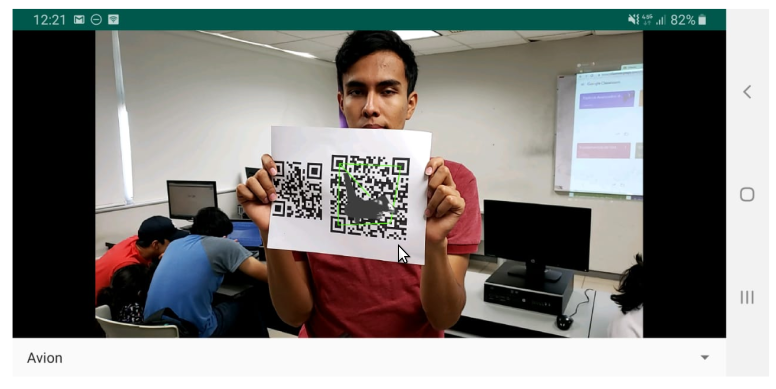
\includegraphics[width=0.98\textwidth]{Figs/SistemaAR2}\\
     \end{center}

\end{column}
\begin{column}{0.5\textwidth}  
    \begin{center}
\begin{itemize}
\end{itemize}

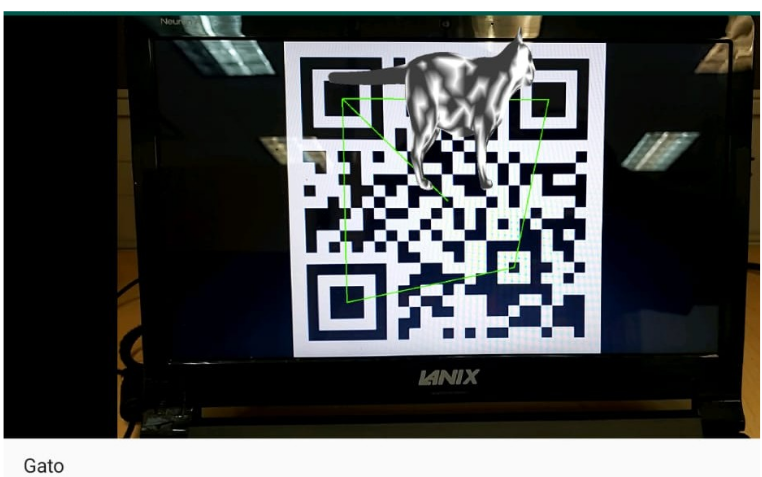
\includegraphics[width=0.98\textwidth]{Figs/SistemaAR3}\\
     \end{center}
\end{column}
\end{columns}



%\end{block} 
\end{frame}


%\renewcommand{\EntradaBibtex}{8994792}
%\begin{frame}{\citetitle{\EntradaBibtex} \footnotemark[1] (1)}



\frame
{
\frametitle{\citetitle{\EntradaBibtex} \footnotemark[1] (1)}

\begin{columns}
\column {0.9\textwidth} 
\begin{itemize}
\item Según la Organización para la Agricultura y la Alimentación (FAO), México es uno de los cinco principales productores de cítricos del mundo. 
\item Los productores de cítricos requieren máquinas clasificadoras capaces de
clasificar frutas según determinadas características (tamaño y color). 
\item La segmentación de imágenes es la primera etapa en una proceso de clasificación. 
\end{itemize}
 \column {0.1\textwidth} 
 \begin{center}
    %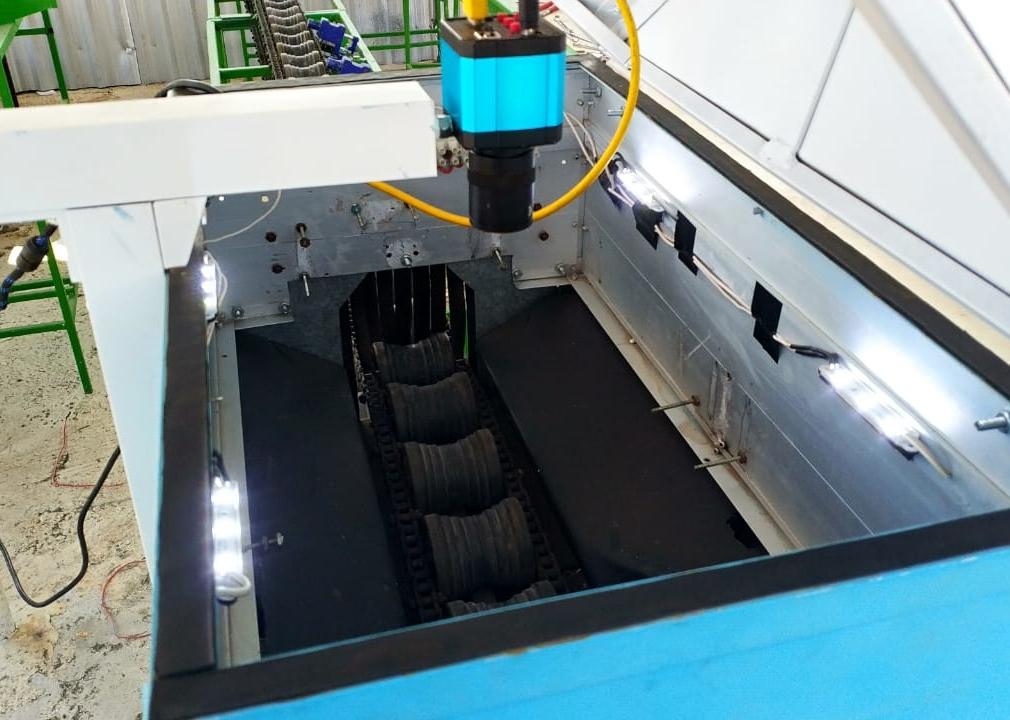
\includegraphics[width=0.9\textwidth]{Figs/2019_Naranjas_cabina}\\
    %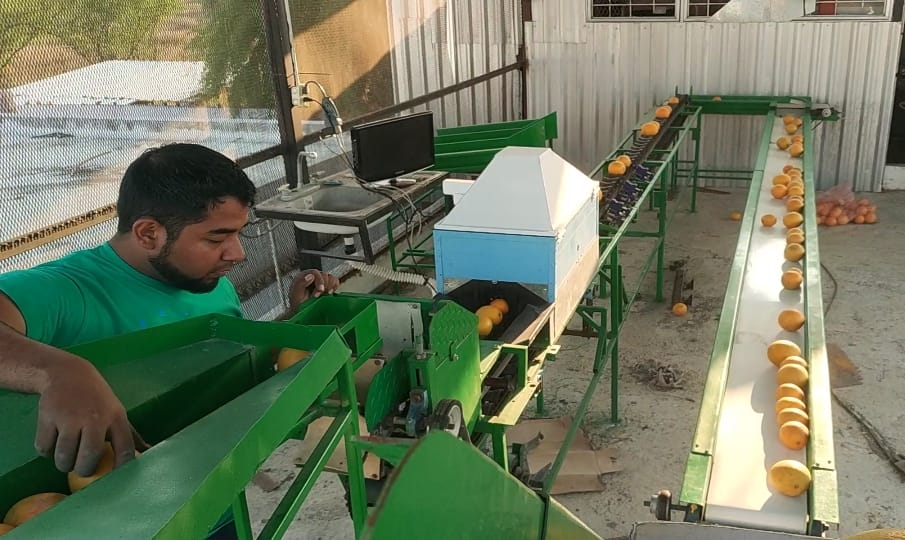
\includegraphics[width=0.9\textwidth]{Figs/2019_Naranjas_Maq}
 \end{center}
\end{columns}

\footnotetext[1]{\fullcite{\EntradaBibtex}}

}

\frame
{
\frametitle{\citetitle{\EntradaBibtex} (2)}
\begin{columns}
 \column {0.5\textwidth} 
 \begin{itemize}
        \item En una primer etapa, se capturaron videos de naranjas pasando a través de la máquina
        \item A partir de esos videos, se propuso un algoritmo para segmentar las naranjas de acuerdo con el color de clasificación deseado
        \item A partir de las naranjas segmentadas, se propuso un modelo  
        \item Ese modelo fue puesto en operación.
 \end{itemize} 
%\begin{center} 
%    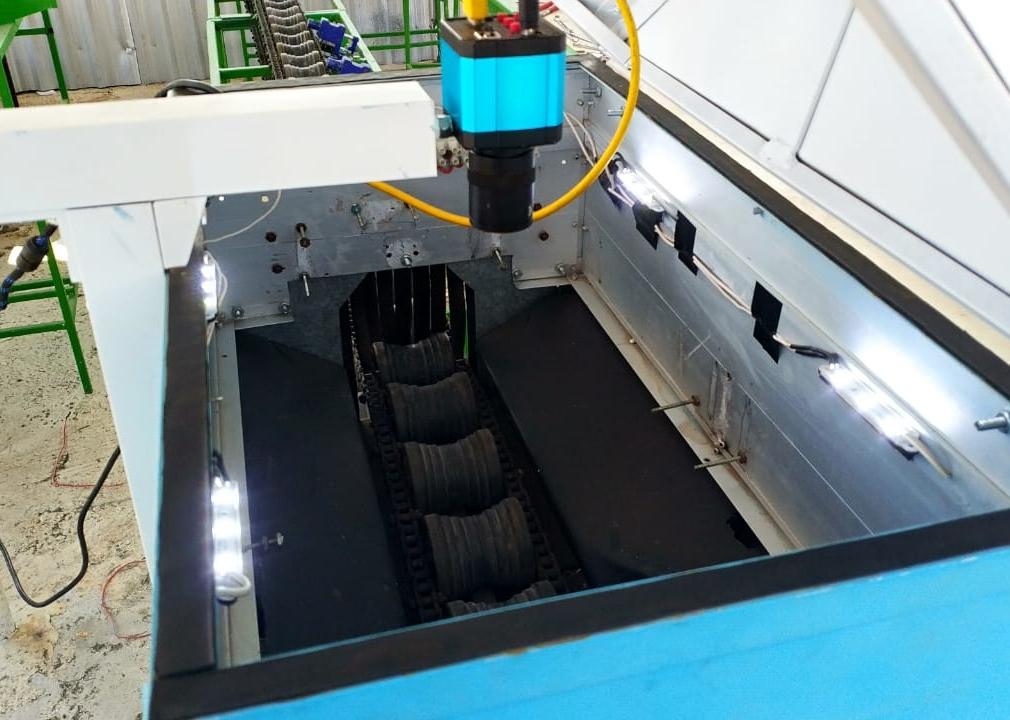
\includegraphics[width=0.7\textwidth]{Figs/2019_Naranjas_cabina}

%\end{center}     
 \column {0.5\textwidth} 
 \begin{center}
    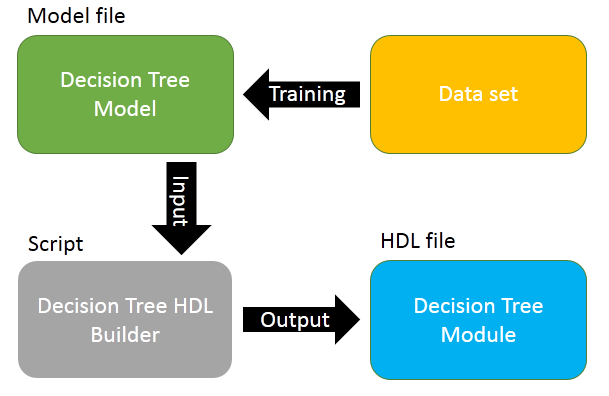
\includegraphics[width=0.7\textwidth]{Figs/2019_Naranjas_weka_overview1}\\
    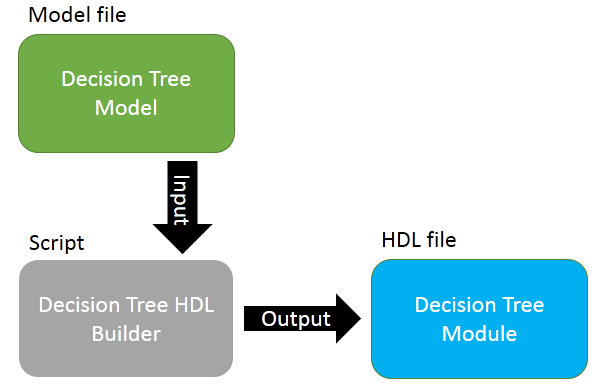
\includegraphics[width=0.7\textwidth]{Figs/2019_Naranjas_weka_overview2}
   \end{center}
\end{columns}


}

\frame
{
\frametitle{\citetitle{\EntradaBibtex} (3)}
\begin{columns}
 \column {0.5\textwidth} 
    \begin{itemize}
        \item Se utilizó una tarjeta Industrial Video Processing Kit (Avnet).
        \item Incluye entrada de video HDMI.
        \item El rendimiento máximo del sistema propuesto es de una tonelada de fruta en 18 minutos.
    \end{itemize}         
 \column {0.5\textwidth} 
 \begin{center}
    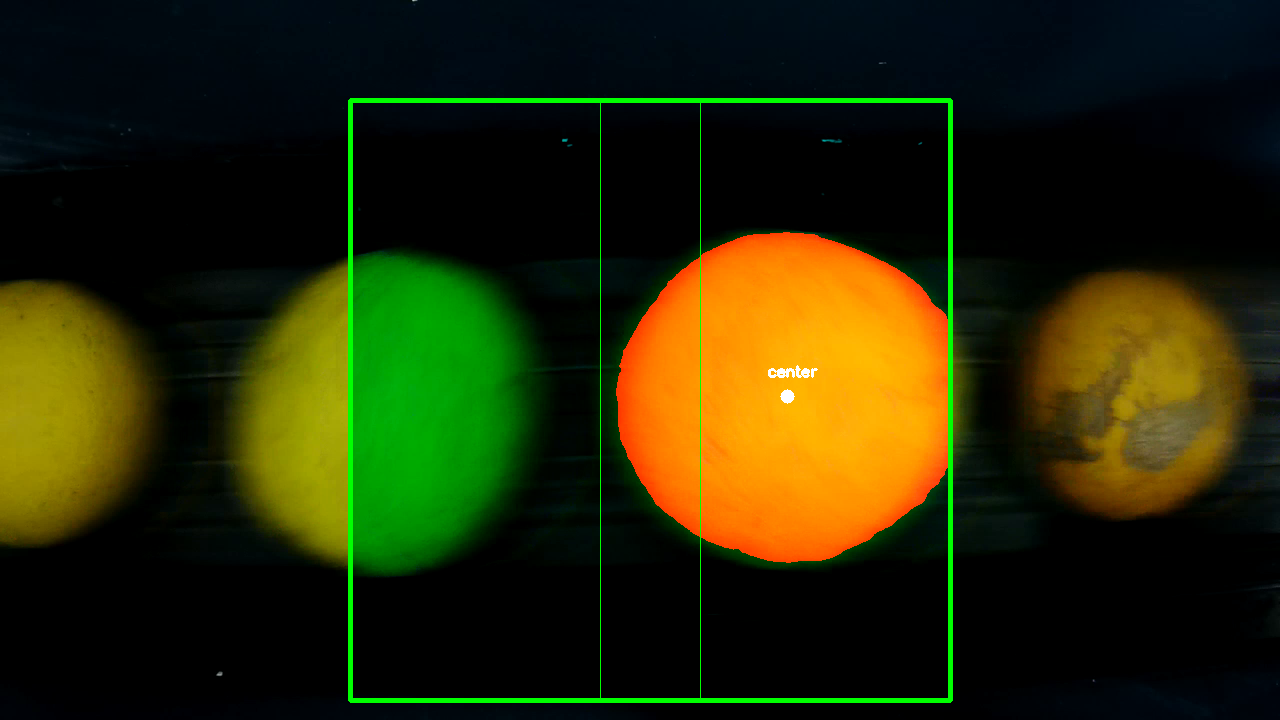
\includegraphics[width=0.7\textwidth]{Figs/2019_Naranjas_Segmentation1}\\
    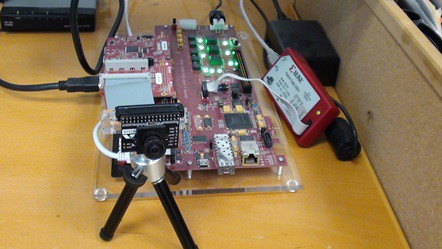
\includegraphics[width=0.7\textwidth]{Figs/2019_Naranjas_Industrial_Video_Processing_Kit}
   \end{center}
\end{columns}
}

%\renewcommand{\EntradaBibtex}{MarcoNuno_Revista_2018_07_00}
\begin{frame}{\citetitle{\EntradaBibtex} \footnotemark[1] (1)}



%\begin{frame}{\citetitle{MarcoNuno_Revista_2018_07_00} \footnotemark (1)}
%\begin{block}{Sistema de Posicionamiento Interior \footnotemark (1)} 
\begin{columns}
\begin{column}{0.5\textwidth}
		\begin{itemize}
		\item Determinar la ubicación de personas/objetos móviles en interiores es un problema abierto
		\item Se propuso un sistema basado en ML, para procesar las intensidades de señal de los puntos de acceso y de esta forma poder conocer la ubicación de manera precisa
		\end{itemize}
\end{column}
\begin{column}{0.3\textwidth}  
    \begin{center}
     %%%%% this is a minipage, so \textwidth is already adjusted to the size of the column
     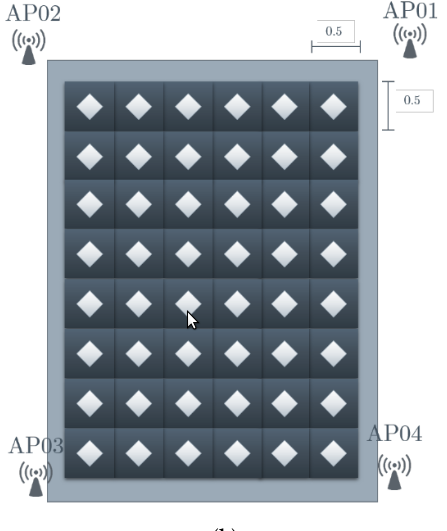
\includegraphics[width=0.85\textwidth]{Figs/IndoorPositionSystem2}
     \end{center}

\end{column}

\begin{column}{0.2\textwidth}  
    \begin{center}
     %%%%% this is a minipage, so \textwidth is already adjusted to the size of the column
     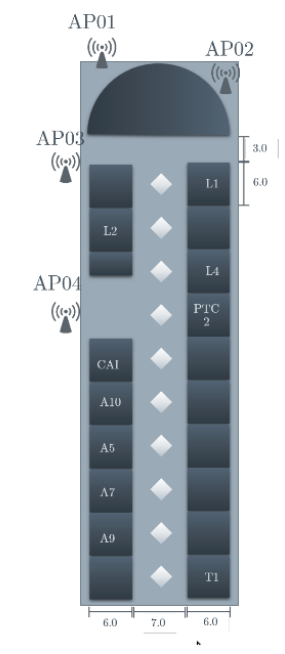
\includegraphics[width=0.8\textwidth]{Figs/IndoorPositionSystem1}
     \end{center}
\end{column}
\end{columns}
%\end{block} 
\footnotetext[1]{\fullcite{\EntradaBibtex}}
\end{frame}

\begin{frame}{\citetitle{\EntradaBibtex} (2)}
%\begin{block}{Sistema de Posicionamiento Interior (2)} 
\begin{columns}
\begin{column}{0.5\textwidth}
  \begin{center}
     %%%%% this is a minipage, so \textwidth is already adjusted to the size of the column
     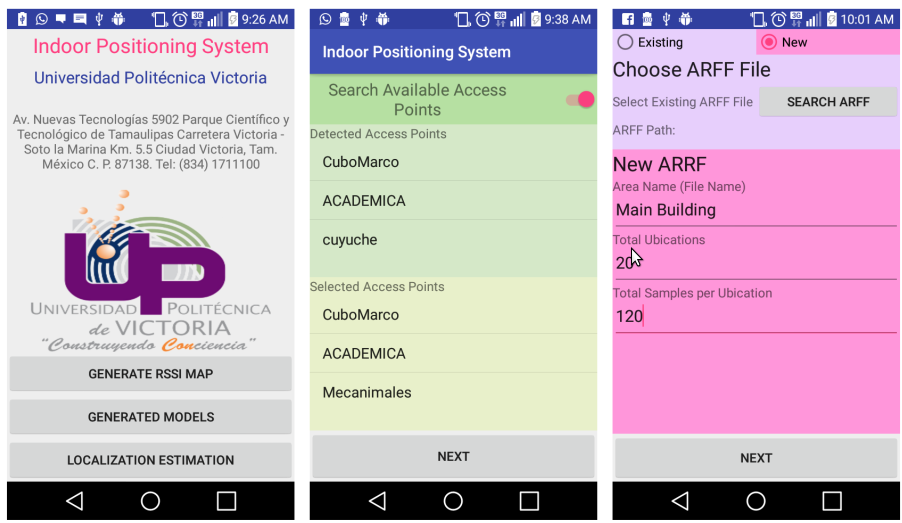
\includegraphics[width=0.95\textwidth]{Figs/IndoorPositionSystem3}
     %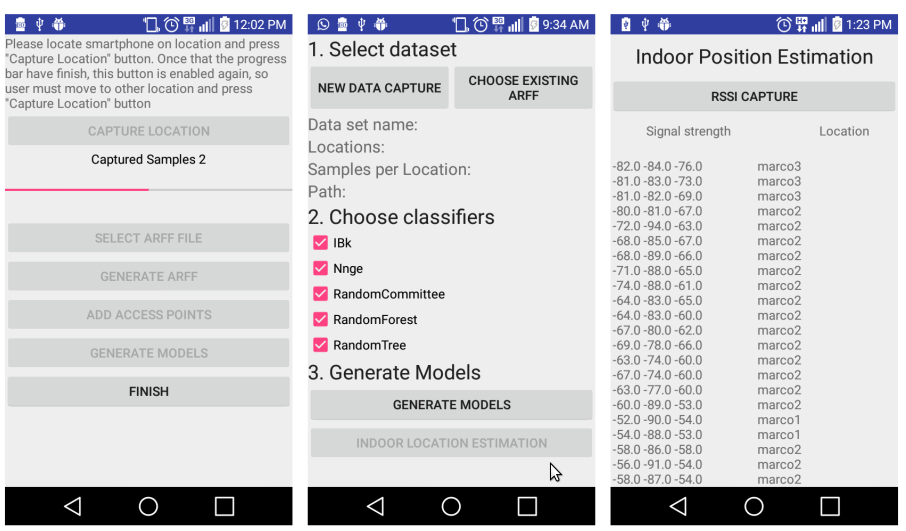
\includegraphics[width=0.5\textwidth]{Figs/IndoorPositionSystem4}
     \end{center}

\end{column}
\begin{column}{0.5\textwidth}
  \begin{center}
     %%%%% this is a minipage, so \textwidth is already adjusted to the size of the column
     %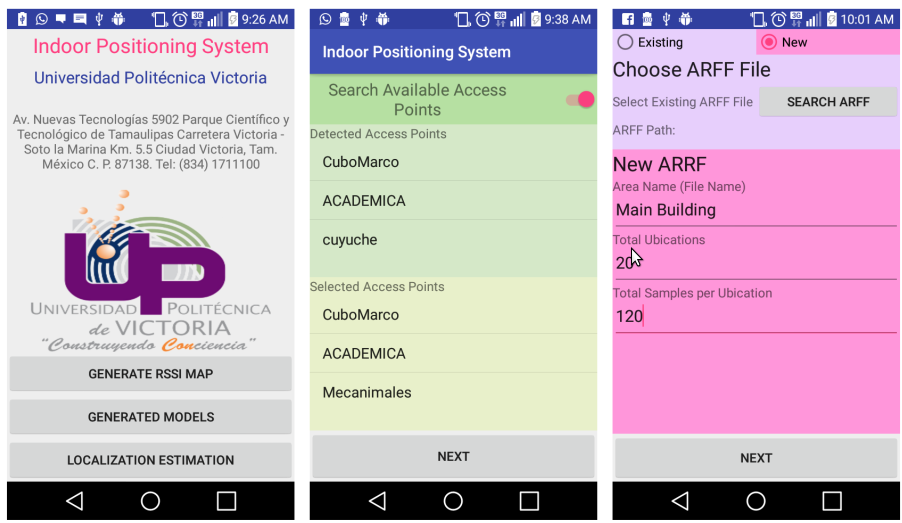
\includegraphics[width=0.5\textwidth]{Figs/IndoorPositionSystem3}
     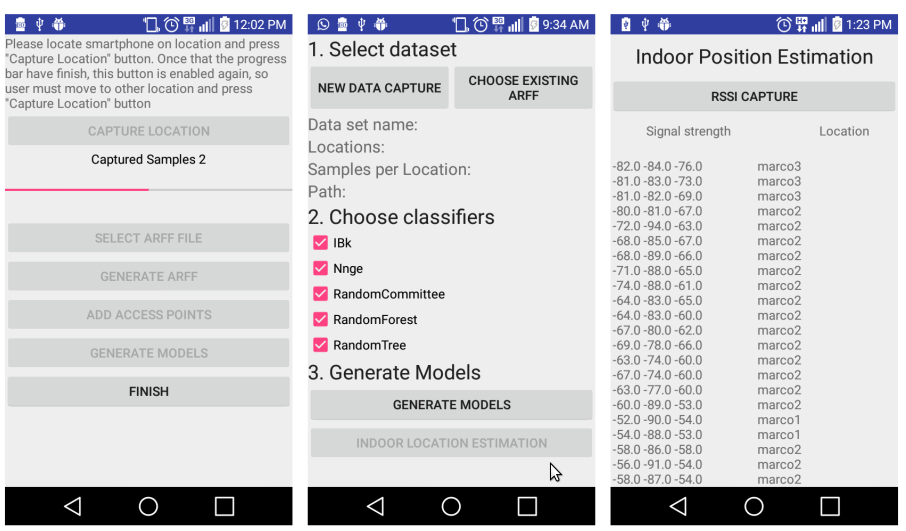
\includegraphics[width=0.95\textwidth]{Figs/IndoorPositionSystem4}
     \end{center}

\end{column}

\end{columns}



%\end{block} 
\end{frame}





%\renewcommand{\EntradaBibtex}{MarcoNuno_CongArbIng_2015_02_00}
\begin{frame}{\citetitle{\EntradaBibtex} \footnotemark[1] (1)}


%\subsection{Aprendizaje automático}
%\begin{frame}{\citetitle{MarcoNuno_CongArbIng_2015_02_00} \footnotemark (1) }
\begin{columns}
\begin{column}{0.4\textwidth}
		Componentes:
		\begin{itemize}
		\item Captura de datos del acelerómetro del teléfono
		\item Procesar los datos empleando algoritmos de ML previamente entrenados, para determinar el tipo de actividad llevada a cabo por el usuario
		\end{itemize}
\end{column}
\begin{column}{0.6\textwidth}  
    \begin{center}
     %%%%% this is a minipage, so \textwidth is already adjusted to the size of the column
     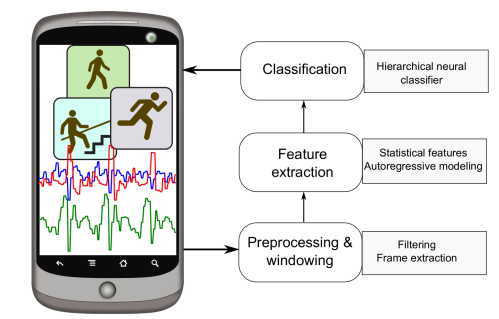
\includegraphics[width=0.8\textwidth]{Figs/DeteccionActividad1}
     \end{center}
\end{column}
\end{columns}
\footnotetext[1]{\fullcite{\EntradaBibtex}}
\end{frame}


\begin{frame}{\citetitle{\EntradaBibtex} (2)}
\begin{columns}
\begin{column}{0.40\textwidth}
		Componentes:
		\begin{itemize}
		\item Se empleo una red neuronal jerárquica
		\item Se midió el desempeño de la bateria y los tiempos de los principales pasos
		\end{itemize}
\begin{center}
     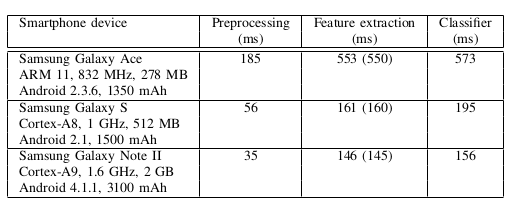
\includegraphics[width=0.7\textwidth]{Figs/DeteccionActividad3}
     
     \end{center}
\end{column}
\begin{column}{0.29\textwidth}  
    \begin{center}
     %%%%% this is a minipage, so \textwidth is already adjusted to the size of the column
     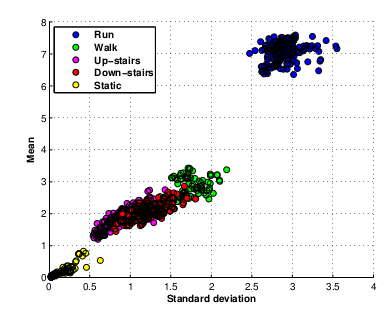
\includegraphics[width=0.97\textwidth]{Figs/DeteccionActividad2}
	%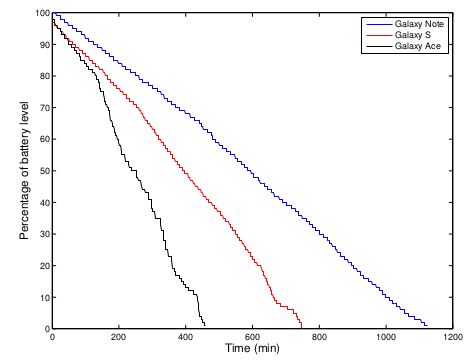
\includegraphics[width=0.7\textwidth]{Figs/DeteccionActividad4}

     \end{center}
\end{column}
\begin{column}{0.29\textwidth}  
    \begin{center}
     %%%%% this is a minipage, so \textwidth is already adjusted to the size of the column
     %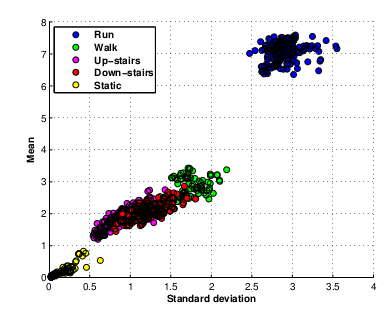
\includegraphics[width=0.7\textwidth]{Figs/DeteccionActividad2}
	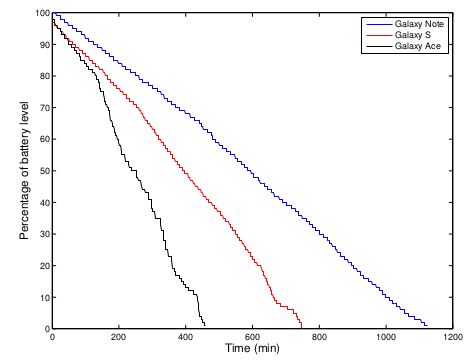
\includegraphics[width=0.97\textwidth]{Figs/DeteccionActividad4}

     \end{center}

\end{column}
\end{columns}
\end{frame}




%\renewcommand{\EntradaBibtex}{MarcoNuno_CongArbIng_2014_07_00}
\begin{frame}{\citetitle{\EntradaBibtex} \footnotemark[1] (1)}



%\section{Proyectos de Investigación}
%\subsection{Visión por Computadora}
%\begin{frame}{\citetitle{MarcoNuno_CongArbIng_2014_07_00}}
\begin{block}{} 
\begin{columns}
\begin{column}{0.4\textwidth}
		\begin{itemize}
		\item Detección y conteo de autómoviles 
		\item Videos capturados desde pueden peatonales
		\item  Detectar regiones de movimiento 
		\end{itemize}
\end{column}
\begin{column}{0.6\textwidth}  
    \begin{center}
     %%%%% this is a minipage, so \textwidth is already adjusted to the size of the column
     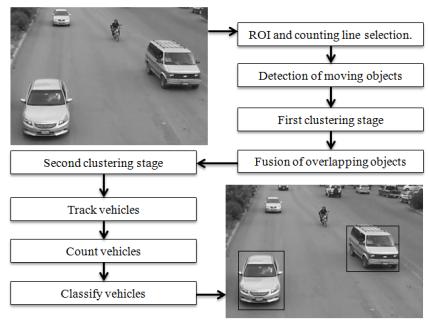
\includegraphics[width=0.70\textwidth]{Figs/TrafficFlow}
     \end{center}
\end{column}
\end{columns}
\end{block} 
%\footnotetext{Raul Humberto Peña-González and Marco Aurelio Nuño-Maganda. \textbf{Computer vision based real-time vehicle tracking and classification system}. In 2014 IEEE 57th International Midwest Symposium on Circuits and Systems (MWSCAS 2014), pages 679–682, Agosto 2014. http://doi.org/10.1109/MWSCAS.2014.6908506ISBN: 978-1-4799-4132-2}
%\footnotetext[1]{\fullcite{MarcoNuno_CongArbIng_2014_07_00}}
\footnotetext[1]{\fullcite{\EntradaBibtex}}
\setcounter{footnote}{0}


\end{frame}

%\begin{frame}{Proyectos de Investigación}
\begin{frame}{\citetitle{\EntradaBibtex} (2)}
\begin{block}{Seguimiento y Clasificación de Vehículos (2)} 
\begin{columns}
\begin{column}{0.4\textwidth}
		\begin{itemize}
		\item Se capturaron videos de diferentes ubicaciones
		\item Se estimó la densidad de flujo de trafico y por tipo de vehiculo
		\item Idea original: detectar conductores usando telefono celular al manejar
		\end{itemize}
\end{column}
\begin{column}{0.6\textwidth}  
    \begin{center}
     %%%%% this is a minipage, so \textwidth is already adjusted to the size of the column
     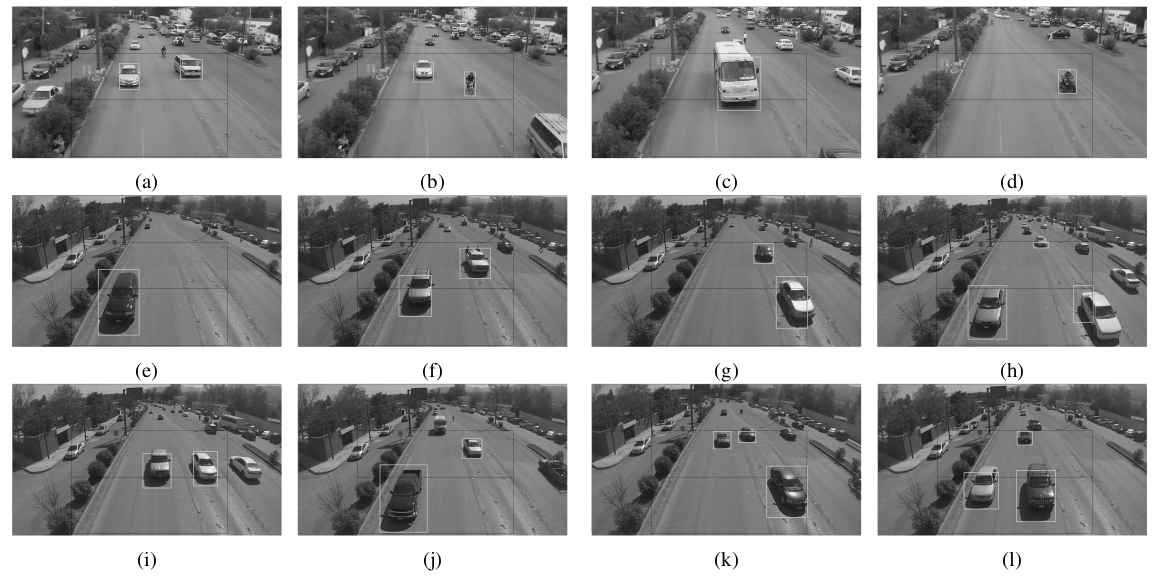
\includegraphics[width=0.8\textwidth]{Figs/TrafficFlow2}
     \end{center}
\end{column}
\end{columns}
\end{block} 
\setcounter{footnote}{0}
\end{frame}






%\renewcommand{\EntradaBibtex}{MarcoNuno_Revista_2014_10_00}
%\begin{frame}{\citetitle{\EntradaBibtex} \footnotemark[1] (1)}


\frame
{
\frametitle{\citetitle{\EntradaBibtex} \footnotemark[1] (1)}
\begin{columns}
\column {0.5\textwidth} 
\begin{itemize}
\item La binarización de imágenes es el proceso que convierte el nivel de grises
para distinguir objetos de regiones del fondo.
\item El umbral adaptativo local ofrece una resultados adecuados pero tiene un alto costo computacional. 
\item Se presenta una implementación de hardware reconfigurable para acelerar el algoritmo de Bernsen.
\end{itemize}
 \column {0.5\textwidth} 
    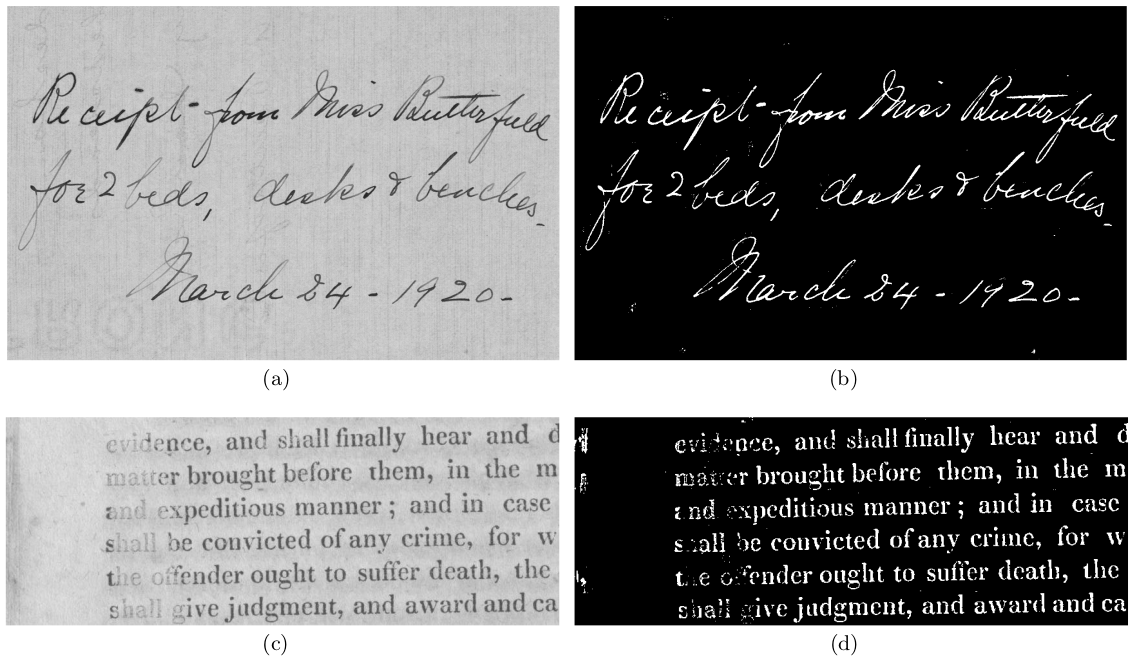
\includegraphics[width=0.9\textwidth]{Figs/2014_Arq_Umbralizacion02}
\end{columns}

\footnotetext[1]{\fullcite{\EntradaBibtex}}
}

\frame
{
\frametitle{\citetitle{\EntradaBibtex}  (2)}
\begin{columns}
\column {0.4\textwidth}
\begin{itemize}
\item El algoritmo de Bernsen requiere dos módulos HGW trabajando en paralelo (max y min filtros).
\item Se emplean memorias BlockRAM (embebida dentro del FPGAs). 
\item La unidad de control genera las direcciones de la memoria externa tanto para leer y almacenar los datos de la memoria de entrada y salida, en función del tamaño de la imagen y del núcleo.
\end{itemize}
\column {0.6\textwidth}
\begin{center}
    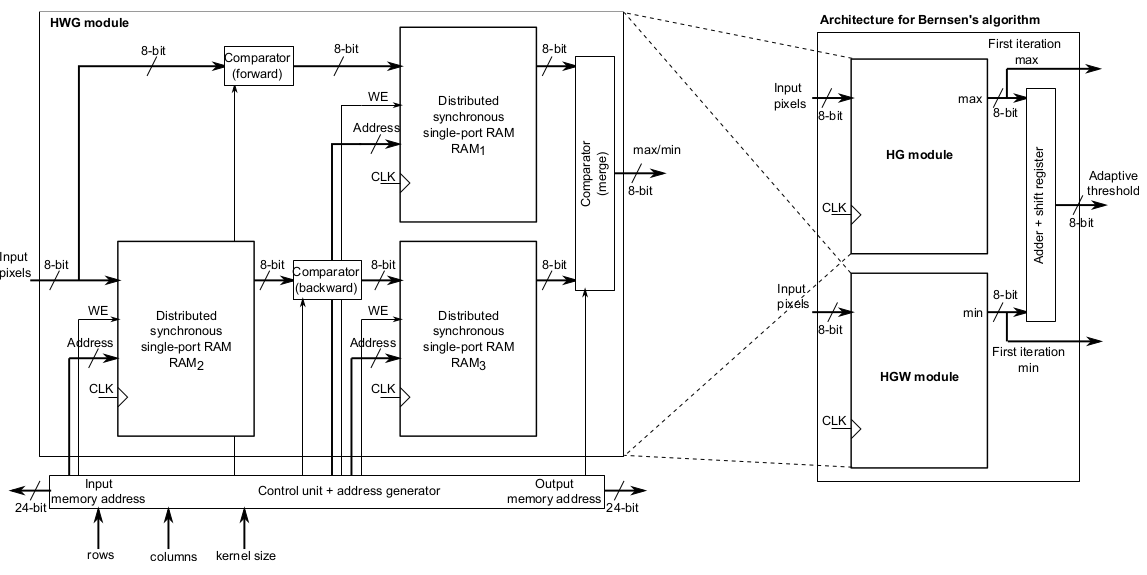
\includegraphics[width=0.99\textwidth]{Figs/2014_Arq_Umbralizacion01}
\end{center}    
\end{columns}
}


\frame
{
\frametitle{\citetitle{\EntradaBibtex}  (3)}
\begin{columns}
\column {0.4\textwidth}
Se implemento un Pipeline de 3 etapas:
\begin{itemize}
\item La primera etapa procesa ventanas de tamaño $k$ a partir de los pixeles de entrada. 
\item La segunda etapa comienza a operar después de $k$ ciclos de reloj.
\item La tercera etapa fusiona una vez que la segunda etapa completa el cálculo de $k/2$ muestras de salida.
\end{itemize}

\column {0.6\textwidth}
\begin{center}
    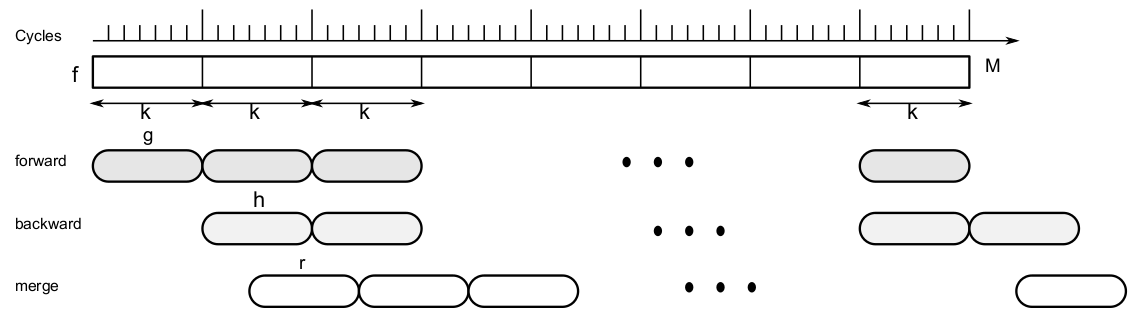
\includegraphics[width=0.99\textwidth]{Figs/2014_Arq_Umbralizacion05}
\end{center}      
\end{columns}

}



\frame
{
\frametitle{\citetitle{\EntradaBibtex} (4)}
\begin{columns}
\column {0.4\textwidth} 
\begin{itemize}
\item FPGAs Atlys y VHDL.

\item Se comparan diferentes tamaños de ventana para una imagen de resolución 2160 $\times$ 1440.
\item Se compararon diferentes tamaños de imagen obteniendo una resolución de video de 30 FPS.
\end{itemize}

 \column {0.3\textwidth} 
    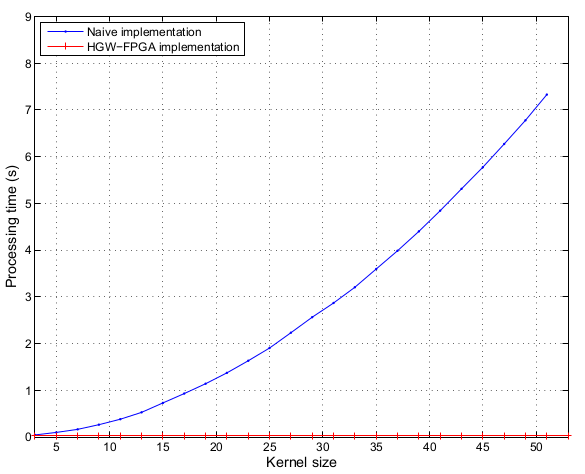
\includegraphics[width=0.9\textwidth]{Figs/2014_Arq_Umbralizacion03}\\
    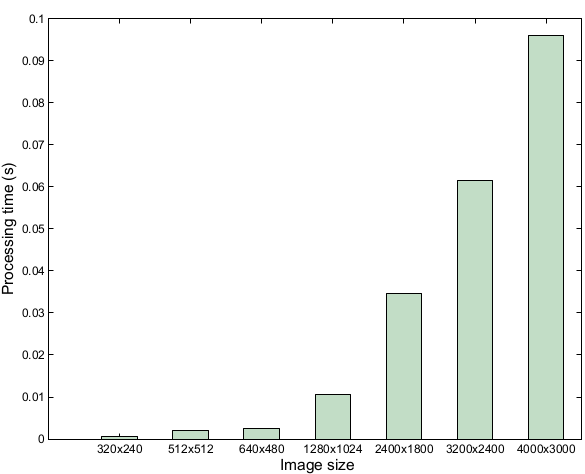
\includegraphics[width=0.9\textwidth]{Figs/2014_Arq_Umbralizacion04}
 \column {0.3\textwidth} 
    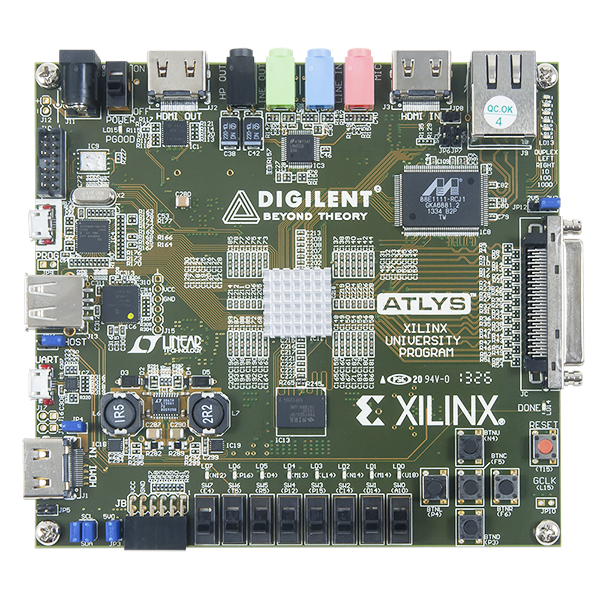
\includegraphics[width=0.9\textwidth]{Figs/atlys-2}\\

\end{columns}

}


%\renewcommand{\EntradaBibtex}{MarcoNuno_CongArbEsp_2014_09_02}
\begin{frame}{\citetitle{\EntradaBibtex} \footnotemark[1] (1)}

%\begin{frame}{\citetitle{MarcoNuno_CongArbEsp_2014_09_02}$^*$  (1)}
\begin{columns}
\begin{column}{0.6\textwidth}
	\begin{itemize}
		\item El estudiante había trabajado en CAPUFE
        \item Tener un mecanismo que evitara que los vehiculos pagaran menos peaje debido a errores de registro
		\item Contar de manera automática el número de ejes de los vehículos
	\end{itemize}
\end{column}
\begin{column}{0.4\textwidth}  
\begin{center}
     \begin{tabular}{c}
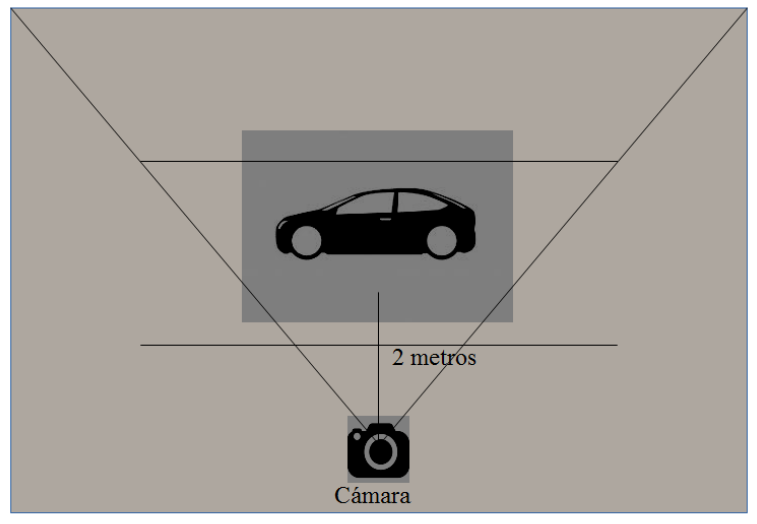
\includegraphics[width=0.68\textwidth]{2014_Llantas/figs/LuisRodolfo1}\\
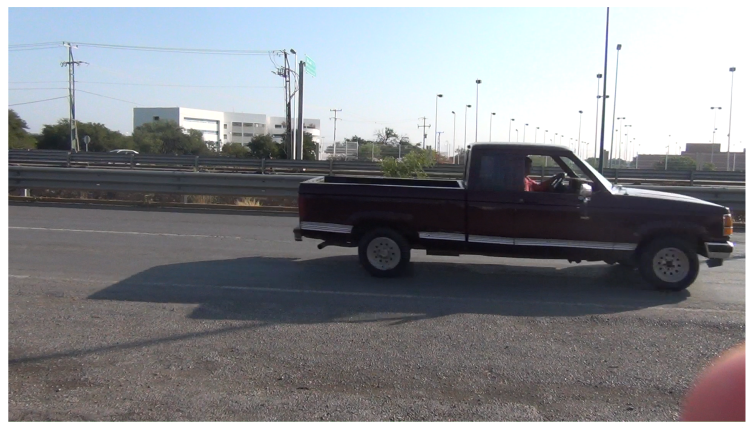
\includegraphics[width=0.68\textwidth]{2014_Llantas/figs/LuisRodolfo2}\\         
      \end{tabular}
\end{center}
\end{column} 
\end{columns} 
\footnotetext[1]{\fullcite{\EntradaBibtex}}
\end{frame}


\begin{frame}{\citetitle{\EntradaBibtex}  (2)}
	\begin{itemize}
        \item Detectar el vehiculo
        \item Acotar las zonas de interes
        \item Aplicar filtrado a los frames individuales
        \item Detectar contornos para reducir la región de búsqueda de las regiones circulares
        \item Aplicar detección de circulos y generar como resultado el número de ejes
	\end{itemize}
\begin{center}
 \begin{tabular}{cccc}
    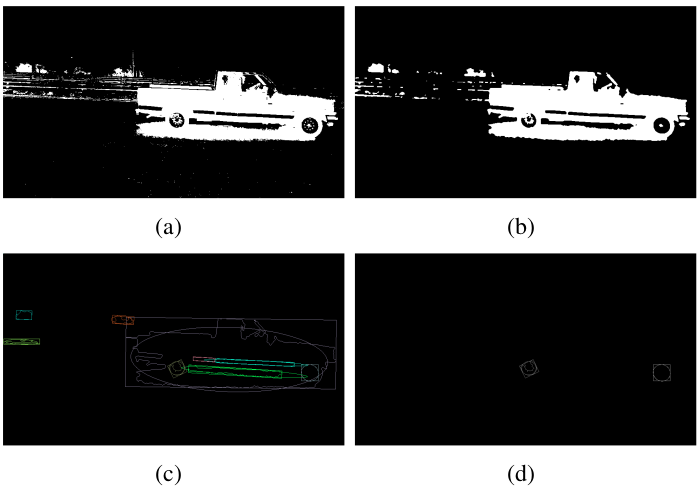
\includegraphics[width=5cm]{2014_Llantas/figs/LuisRodolfo5}
    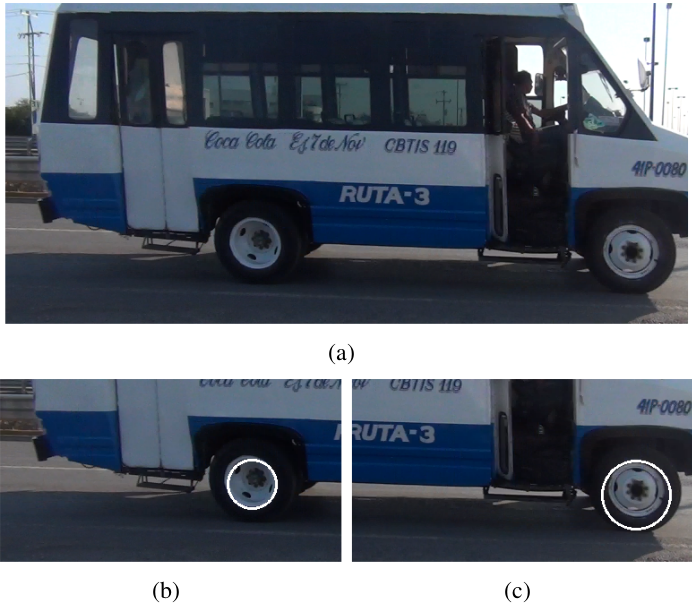
\includegraphics[width=4cm]{2014_Llantas/figs/LuisRodolfo3}
    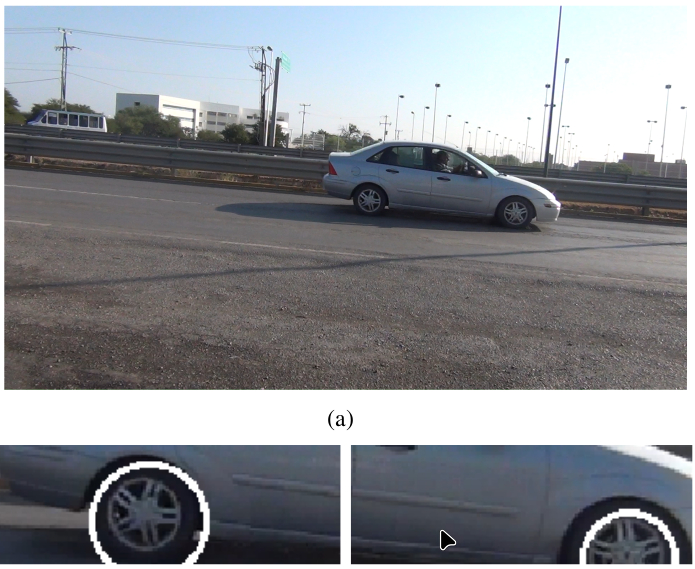
\includegraphics[width=4cm]{2014_Llantas/figs/LuisRodolfo4}
  \end{tabular}
\end{center}

\end{frame}







%\renewcommand{\EntradaBibtex}{MarcoNuno_CongArbIng_2014_12_00X}
\begin{frame}{\citetitle{\EntradaBibtex} \footnotemark[1] (1)}



%\begin{frame}{\citetitle{MarcoNuno_CongArbIng_2014_12_00X}  \footnotemark (1)}
\begin{columns}
\begin{column}{0.4\textwidth}
		Componentes:
		\begin{itemize}
		\item Una cama para libros abiertos
		\item Un mecanismo para cambiar de página a través de uns servomotores
		\item Un sistema de iluminación 		
		\end{itemize}
\end{column}
\begin{column}{0.6\textwidth}  
    \begin{center}
     %%%%% this is a minipage, so \textwidth is already adjusted to the size of the column
     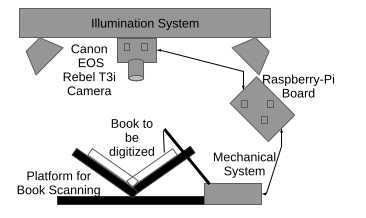
\includegraphics[width=0.8\textwidth]{Figs/BookScanner1}
     \end{center}
\end{column}
\end{columns}

\footnotetext[1]{\fullcite{\EntradaBibtex}}
\end{frame}


\begin{frame}{\citetitle{\EntradaBibtex} (2)}
%\begin{block}{Prototipo para Digitalizar Libros (2)} 
\begin{columns}
\begin{column}{0.6\textwidth}
		\begin{itemize}
		\item Una cámara de alta definición para capturar fotografías de ambas páginas
		\item Una computadora Embebida con la cámara conectada para procesar la imágen e integrar el libro digitalizado en formato PDF.
		\item Nucleo: Un sistema de visión para detectar automáticamente los límites de las páginas y cortas para generar el documento
		\end{itemize}
\end{column}
\begin{column}{0.4\textwidth}  
    \begin{center}
     %%%%% this is a minipage, so \textwidth is already adjusted to the size of the column
     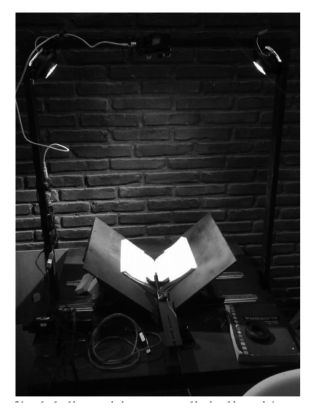
\includegraphics[width=0.8\textwidth]{Figs/BookScanner2}
     \end{center}
\end{column}
\end{columns}
%\end{block} 
\end{frame}


\begin{frame}{\citetitle{\EntradaBibtex} (3)}
%\begin{block}{} 
\begin{columns}
\begin{column}{0.5\textwidth}
%   some text here some text here some text here some text here some text here
     \begin{center}
     %%%%% this is a minipage, so \textwidth is already adjusted to the size of the column
     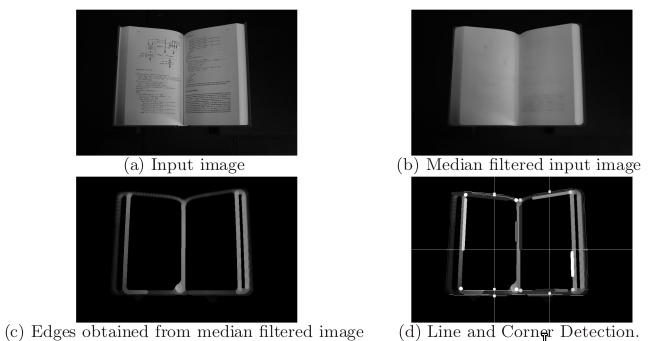
\includegraphics[width=0.88\textwidth]{Figs/BookScanner3}
     \end{center}

\end{column}
\begin{column}{0.5\textwidth}  
    \begin{center}
     %%%%% this is a minipage, so \textwidth is already adjusted to the size of the column
     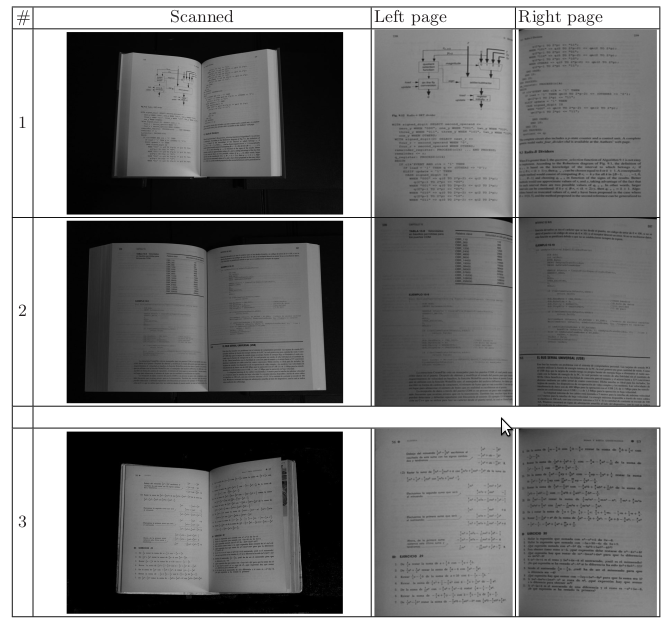
\includegraphics[width=0.88\textwidth]{Figs/BookScanner4}
     \end{center}
\end{column}
\end{columns}
%\end{block} 
\end{frame}



%\renewcommand{\EntradaBibtex}{MarcoNuno_CongArbEsp_2013_11_01}
\begin{frame}{\citetitle{\EntradaBibtex} \footnotemark[1] (1)}

%\begin{frame}{\citetitle{MarcoNuno_CongArbEsp_2013_11_01} \footnotemark (1)}
%\begin{block}{Prototipo de un entorno virtual para un robot de servicio\footnotemark } 
\begin{columns}
\begin{column}{0.52\textwidth}
    \begin{center}

\begin{itemize}
\item Prototipo SerBot I
\item Modelo 3D del Robot
\item Modelo 3D del entorno
\item Plataforma: PC de escritorio
\end{itemize}
     \end{center}

\end{column}
\begin{column}{0.48\textwidth}  
    \begin{center}
\begin{itemize}
\end{itemize}
     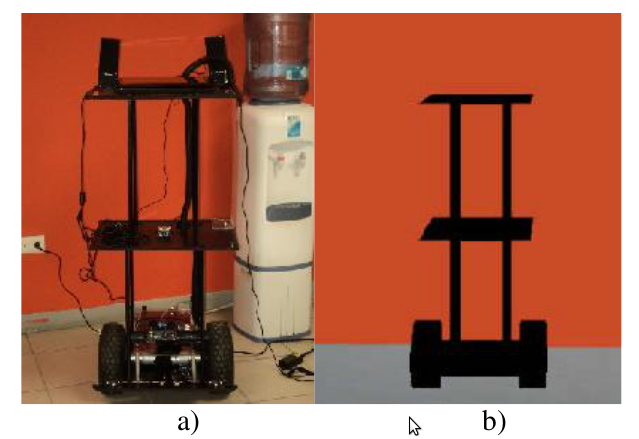
\includegraphics[width=0.9\textwidth]{Figs/SerbotI_A}\\
     \end{center}
\end{column}
\end{columns}


%\end{block} 
\footnotetext[1]{\fullcite{\EntradaBibtex}}
%\\setcounter{footnote}{0}
\end{frame}



\begin{frame}{\citetitle{\EntradaBibtex}  (2)}
%\begin{block}{Prototipo de un entorno virtual para un robot de servicio (2)} 
\begin{columns}
\begin{column}{0.60\textwidth}
    \begin{center}

\begin{itemize}
\item A partir de los planos de los edificios y de las fotografías, se construyó un prototipo del entorno
\item El plano permitía determinar en donde esta ubicadas paredes y puertas
\end{itemize}
     \end{center}

\end{column}
\begin{column}{0.38\textwidth}  
    \begin{center}
\begin{itemize}
\end{itemize}
     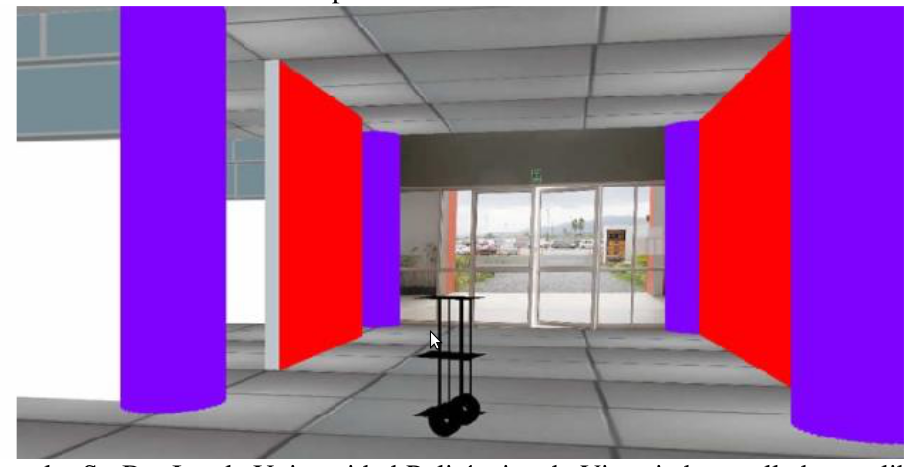
\includegraphics[width=0.9\textwidth]{Figs/SerbotI_B}\\
     \end{center}
\end{column}
\end{columns}
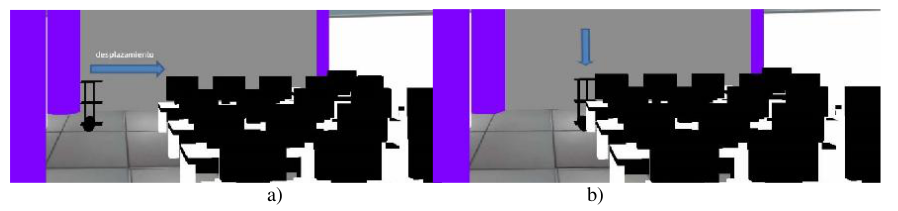
\includegraphics[width=0.8\textwidth]{Figs/SerbotI_C}\\


%\end{block} 
\end{frame}


\begin{frame}{\citetitle{\EntradaBibtex}  (3)}
%\begin{block}{Prototipo de un entorno virtual para un robot de servicio (2)} 
\begin{columns}
\begin{column}{0.48\textwidth}
    \begin{center}

\begin{itemize}
\item Se implementaron controles para movimiento del Robot y del cambio de Vista
\item En robot podía avanzar hacia adelante (moviendo las ruedas en la misma dirección) pero girar moviendo una rueda y dejando la otra quieta
\end{itemize}
     \end{center}

\end{column}
\begin{column}{0.52\textwidth}  
    \begin{center}
\begin{itemize}
\end{itemize}
     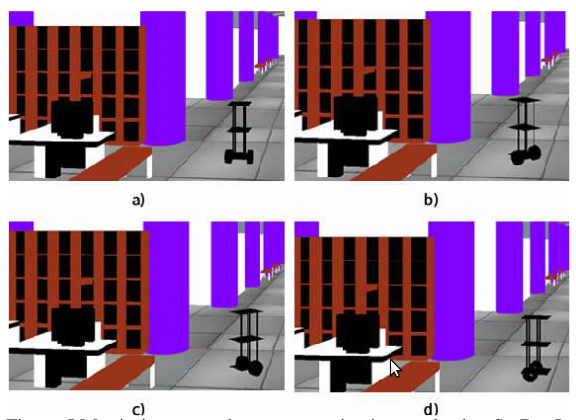
\includegraphics[width=0.9\textwidth]{Figs/SerbotI_D}\\
     \end{center}
\end{column}
\end{columns}
%\end{block} 
\end{frame}

%% SCRIPT
% The next project in this presentation is named "A Novel Strategy for Image Segmentation of Latent Fingerprints~}." 
% The results of this project were published on a confence paper in 2012. 
% Slide 1




% Slide 2


% Slide 3

% Conclusion

%\renewcommand{\Titulo}{A Novel Strategy for Image Segmentation of Latent Fingerprints~}

\renewcommand{\EntradaBibtex}{MarcoNuno_CongArbIng_2012_02_00}
\begin{frame}{\citetitle{\EntradaBibtex} \footnotemark[1] (1)}


%\begin{frame}{\citetitle{MarcoNuno_CongArbIng_2012_02_00} \footnotemark (1)}

\note[item]{\scriptsize  A Fingerprint is an impression or mark made on a surface by a person's fingertip, especially as used for identifying individuals from the unique pattern of whorls and lines.}
\note[item]{\scriptsize  The main stages of AFIS involves:  1. Capture of the fingerprint image. 2. Image processing 3. Feature extraction  4. Matching 5. Storing}
%\note[item]{\scriptsize  The adequate processing of the fingerprint image is a relevant task for the recognition process. If the image is not processed correctly, false characteristics could be obtained in the feature extraction phase or important information could be discarded, increasing the probability that the identification of the individual and the system fails.}
\note[item]{\scriptsize  In this project a new strategy for segmentation of latent fingerprints is proposed, based on the use of gradients and the detection of regions in the image. Our algorithm is able to detect the area of interest in the fingerprint eliminating spots, shadows, noise, etc., and adapting itself to the different conditions in the image.}

	\begin{itemize}
\item Automatic Fingerprint Identification Systems (AFIS) are very important due to their security applications.
\item The main stages of AFIS involves several image processing operators. 
\item The adequate processing of the fingerprint image is important 

	\end{itemize}
	    \begin{center}
    \begin{tabular}{c}
        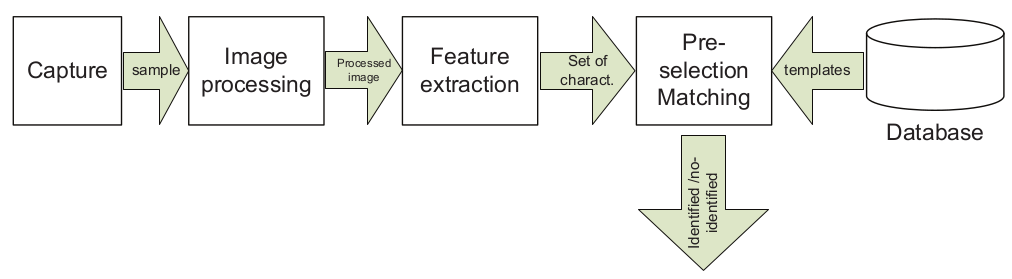
\includegraphics[width=0.75\linewidth]{Figs/Fingerprint1}\\
    \end{tabular}
    	    \end{center}

\footnotetext[1]{\fullcite{\EntradaBibtex}}
\end{frame}

\begin{frame}{\citetitle{\EntradaBibtex} (2)}
Estrategia propuesta:
\begin{columns}
		\begin{column}{0.48\textwidth}

		    \begin{enumerate} \small
		        \item Compute gradient and gradient magnitude.
                \item Normalize the pixel values to the range [0 255].
                \item Binarize the normalized image.
                \item Apply a mean filter to the binarized image            
            \end{enumerate}  
        \end{column}          
		\begin{column}{0.48\textwidth}
		    \begin{enumerate} \small
				\setcounter{enumi}{4}
    \item Binarize the image obtained
                \item Find the label matrix.
                \item Find the label with the high number of instances.
                \item Detect the largest region of interest.			
            \end{enumerate}  

        \end{column}
\end{columns}


\note[item]{\scriptsize  The gradient is a tool widely used for detecting edges in
an image. 
}

%\note[item]{\scriptsize This normalization is performed executing the following steps: ii) Find the minimum intensity value. ii) Subtract the minimum intensity value to each pixel in the image. iii) Find the maximum intensity value in the image and divide 255 by it. iv) Multiply each intensity value by the result obtained in the previous step.}

\note[item]{\scriptsize Binarize the normalized image using as threshold the
mean value of the gradient magnitude image.}

%\note[item]{\scriptsize A new median value is computed from the binarized image, which will be used as threshold for future binarization}

\note[item]{\scriptsize  The labeling algorithm allows to identify zones in the input image formed by interconnected pixels in a binary image that belongs to the foreground (object of interest).}

%\note[item]{\scriptsize Excluding labels that belongs to the background.}

%\note[item]{\scriptsize Send to the background the rest of the detected regions.}

		
\begin{center}
     \begin{tabular}{c}
         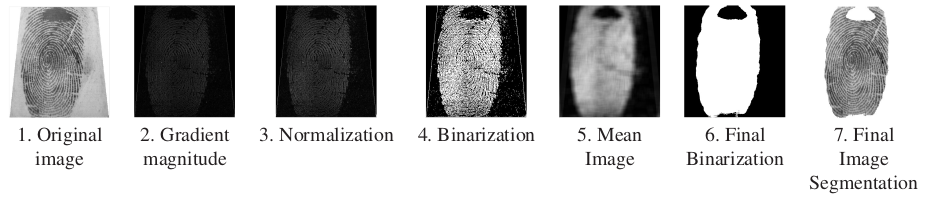
\includegraphics[width=0.95\linewidth]{Figs/Fingerprint2}\\
          \end{tabular}
\end{center}


\end{frame}

\begin{frame}{\citetitle{MarcoNuno_CongArbIng_2012_02_00} (2)}

\note[item]{\scriptsize  In this slide we show the different stages of the segmentation strategy proposed in this work. }

\note[item]{\scriptsize The resolution of images used in this work is 328 × 364 pixels .}

%Resultados
\begin{columns}
		\begin{column}{0.48\textwidth}
		We compared the proposed method against the most representative segmentation algorithms
		\begin{itemize}
		\item Our method achieves the better results, producing as result of
segmentation a single region and discarding no relevant information in the latent fingerprint.
    \item Images that have high contrast between the peaks and valleys that remark the borders in the image performs better.
				\end{itemize}
        \end{column}
				\begin{column}{0.48\textwidth}
				
\begin{center}
     \begin{tabular}{c}
              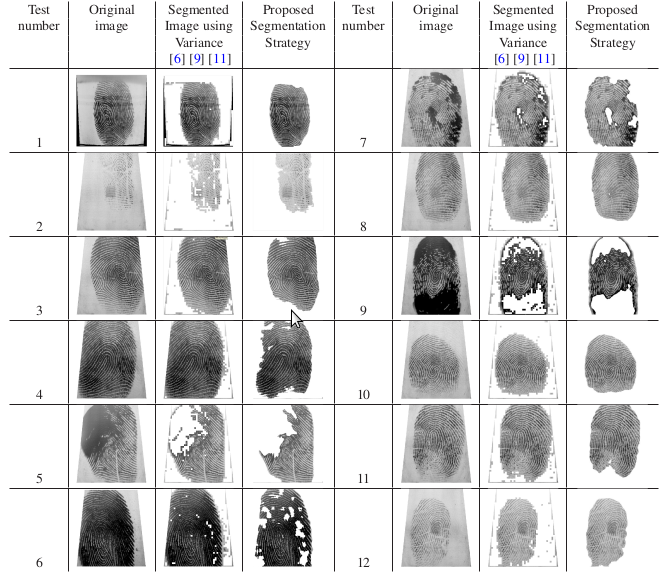
\includegraphics[width=0.85\textwidth]{Figs/Fingerprint3}
          \end{tabular}
\end{center}
				\end{column}
								\end{columns}

\end{frame}








%% SCRIPT
% The next project in my presentation is named "Physician software interface for an intelligent glucose monitor."

%\renewcommand{\Titulo}{Physician software interface for an intelligent glucose monitor~}

%\begin{frame}{\citetitle{MarcoNuno_CongArbIng_2012_01_00}\footnotemark (1)}

\renewcommand{\EntradaBibtex}{MarcoNuno_CongArbIng_2012_01_00}
\begin{frame}{\citetitle{\EntradaBibtex} \footnotemark[1] (1)}

% Slide 1
\note[item]{\scriptsize Los pacientes con diabetes tipo 1 o 2 requieren checar varias veces al día sus niveles de glucosa } 
\note[item]{\scriptsize Se requiere de un dispositivo que recomiende dosis de insulina bsado en los parametros fisiológicos del paciente y de los carbohidratos consumidos }
\note[item]{\scriptsize Se desarrolló una plataforma We developed a medical surveillance platform with two components}
\note[item]{\scriptsize The first component is an Intelligent Glucose Monitor (IGM)
with the hardware layer and electronics needed to interact with glucose-sensing strips}
\note[item]{\scriptsize The second one is a Physician software interface (PSI) to configure and extract information from an Intelligent Glucose Monitor (IGM). }

	\begin{itemize}
\item Los pacientes con diabetes tipo 1 o 2 requieren checar varias veces al día sus niveles de glucosa 
\item La mayoría de los dispositivos comerciales almacenan el historia de lecturas de glucosa en el dispositivo.
\item Se desarrollo un monitor de glucosa inteligente (IGM).
\item El médico puede obtener los datos del dispositivo a través de una aplicación de esritorio (PSI).
\item Herramientas:
	\begin{itemize}
		\item C++ para el IGM.
		\item Java para el PSI.
	\end{itemize}
	\end{itemize}
\footnotetext[1]{\fullcite{\EntradaBibtex}}
\end{frame}

%\begin{frame}{\citetitle{MarcoNuno_CongArbIng_2012_01_00} (2)}
\begin{frame}{\citetitle{\EntradaBibtex} (2)}


\begin{columns}
		\begin{column}{0.48\textwidth}
		    Componentes
		    \begin{itemize}
		        \item Microcontrolador.
                \item LCD Display.
                \item Sensor de Glucosa.
                \item Real time clock.
                \item Interfaz USB .
                \item Interfaz para obtenr datos de las tiras de sensado de glucosa.
            \end{itemize}
            Un menú permite al usuuario interactuar con el IGM. 
		\end{column}
		
				\begin{column}{0.48\textwidth}
\begin{center}
     \begin{tabular}{c}
         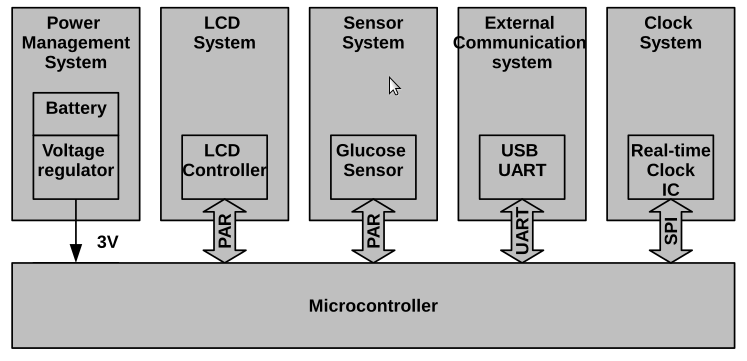
\includegraphics[width=0.85\linewidth]{Figs/IntelligentGlucometer1}\\
         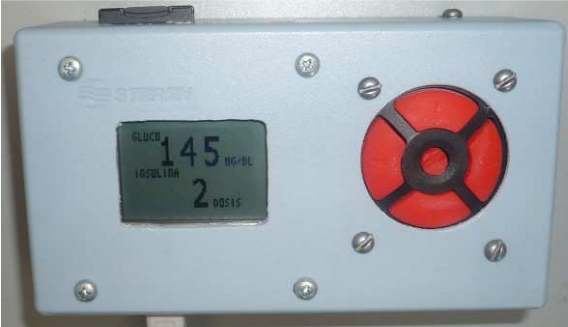
\includegraphics[width=0.75\linewidth]{Figs/IntelligentGlucometer3}\\
          \end{tabular}
\end{center}
		\end{column}
				\end{columns}

\end{frame}



%\begin{frame}{\citetitle{MarcoNuno_CongArbIng_2012_01_00} (3)}
\begin{frame}{\citetitle{\EntradaBibtex} (3)}
\begin{columns}
		\begin{column}{0.48\textwidth}
		La interfaz de médico permite las siguientes acciones:
		\begin{itemize}
		\item Obtener y almacenar los datos de las lecturas de glucosa del IGM, y generar informes.
		\item Configurar el perfil médico del paciente, en base a esto, el IGM recomienda las dosis de insulina		
        \end{itemize}
				\end{column}
				\begin{column}{0.48\textwidth}
\begin{center}
     \begin{tabular}{c}
         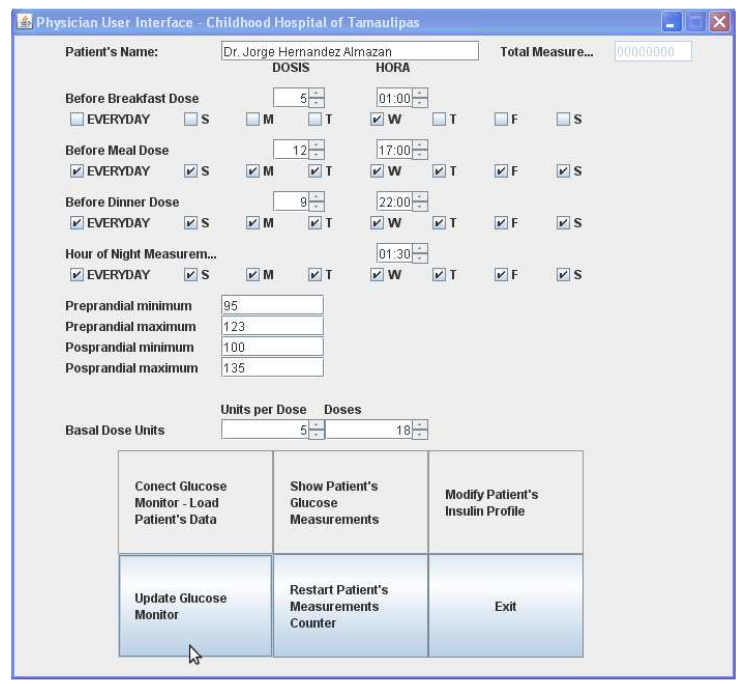
\includegraphics[width=0.86\textwidth]{Figs/IntelligentGlucometer4}
          \end{tabular}
\end{center}
		\end{column}
				\end{columns}
\end{frame}



%
\renewcommand{\EntradaBibtex}{MarcoNuno_Revista_2011_06_00}
%\begin{frame}{\citetitle{\EntradaBibtex} \footnotemark[1] (1)}

\frame
{
\frametitle{\citetitle{\EntradaBibtex} \footnotemark[1] (1)}
%\AtNextCite{\defcounter{maxnames}{99}}\fullcite{\Cita} 

\begin{itemize}
\item Las proteínas y los péptidos son componentes fundamentales de las células que llevan a cabo una importante función biológica.

\item La identificación de péptidos antibacterianos catiónicos selectivos (SCAP), que pueden utilizarse en el tratamiento de diferentes enfermedades.

\item El cálculo de las propiedades fisicoquímicas es considerado un problema informático de alto rendimiento.

\item Se implementaron una arquitectura hardware que evalua cuatro propiedades fisicoquímicas útiles en la identificación de secuencias de péptidos con potencial actividad antibacteriana selectiva.
\end{itemize}

\footnotetext[1]{\fullcite{\EntradaBibtex}}
}

\frame{
\frametitle{\citetitle{\EntradaBibtex} (2)}
\begin{columns}
    \column {0.5\textwidth}
    \begin{itemize}
    \item Se propone una arquitectura hardware con 4 bloques básicos, cada bloque realiza cada uno de los 4 fisicoquímicos cálculos de propiedades.
    \item Hydrophobicity Hardware Module (HHM).
% La hidrofobicidad es la propiedad física de una molécula que aparentemente es repelida por una masa de agua.    
    \item Mean Net Charge Hardware Module (MNCHM).
% A protein's net charge depends on the number of charged amino acids it contains and the pH of its environment    
    \item Isoelectric Point Charge Hardware Module (IPCHM).
%The isoelectric point (pI) is the point at which the net charge on a molecule is zero.     
    \item Helical Hydrophobic Moment Hardware Module (HHMHM).
% The helical hydrophobic moment: a measure of the amphiphilicity of a helix.
% Amphiphilicity: Molecules having both water loving and repelling property.    
\end{itemize}
    
    \column {0.5\textwidth} 
    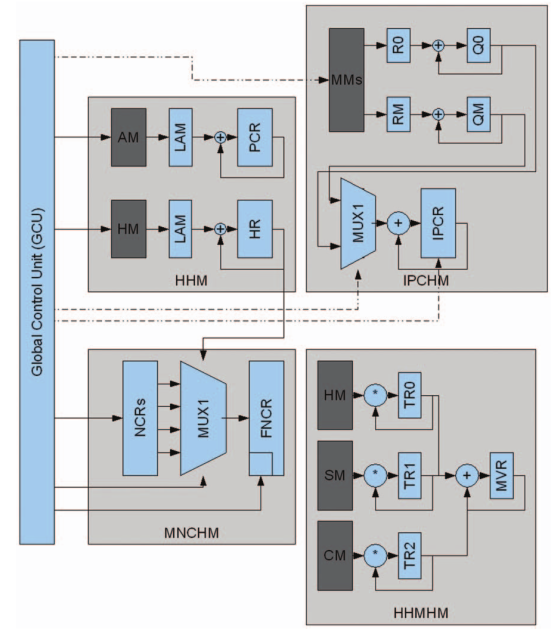
\includegraphics[width=0.9\textwidth]{Figs/2021_Peptidos01}
\end{columns}     
}

\frame{
\frametitle{\citetitle{\EntradaBibtex} (3)}
\begin{columns}
    \column {0.5\textwidth}


\begin{itemize}
\item Cada secuencia de péptidos estaba representada por un punto fijo número y generado por la placa FPGA, eliminando así el sobrecarga debido a la comunicación de datos CPU-FPGA.

\item Los péptidos usados en este estudio estan formados por cadenas de 9 aminoácidos (20 posibles aminoacidos diferentes, 5 bits para su codificación), implicando 45 bits para cada péptido. 

\item Para generar todas las secuencias de péptidos generadas y evaluadas en la tarjeta FPGA se utilizó un contador binario.

	   
\end{itemize}
    
    
    \column {0.5\textwidth} 
\begin{itemize}    
    \item La implementación tiene la misma precisión que la versión de software del mismo.
    \item Individualmente, cada uno de los 4 cálculos de propiedades fisicoquímicas se aceleraron de 17 a 195 veces con la implementación FPGA propuesta.
\end{itemize}
   \begin{center} 
    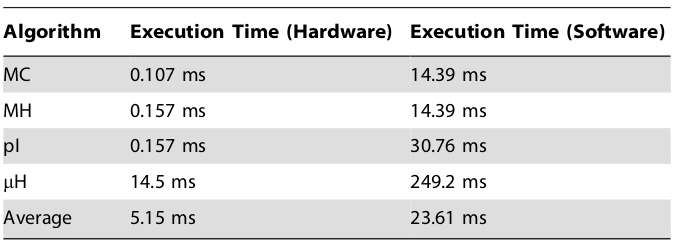
\includegraphics[width=0.9\textwidth]{Figs/2021_Peptidos02}
    \end{center} 
\end{columns}     
}

%
\renewcommand{\EntradaBibtex}{MarcoNuno_CongArbIng_2009_06_00}
%\begin{frame}{\citetitle{\EntradaBibtex} \footnotemark[1] (1)}



\frame
{
\frametitle{\citetitle{\EntradaBibtex} \footnotemark[1] (1)}
\begin{columns}
    \column {0.75\textwidth}
\begin{itemize}    
\item Las Redes Neuronales Pulsantes (SNN) son tema de investigación relevante debido a la plausibilidad biológica mostrada por estos modelos. 
\item Un estudio comparativa acerca de implementaciones en FPGA de clásicos y pulsantes arrojó que estos últimos son menos voraces respecto al uso de hardware en compración con los modelos de segunda generación.
\item Dependiendo del umbral de la neurona, cuando el potencial neuronal alcanza es alcanzado la neurona emite un pico de salida. 
\end{itemize}    
    \column {0.25\textwidth} 
    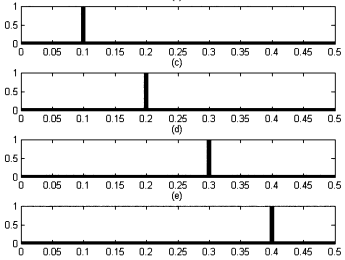
\includegraphics[width=0.9\textwidth]{Figs/2009_BackPropagationFF05}\\
    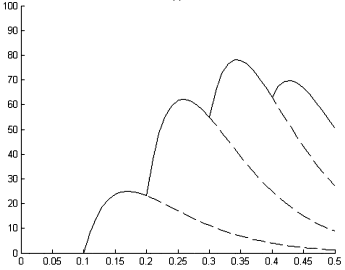
\includegraphics[width=0.9\textwidth]{Figs/2009_BackPropagationFF06}
\end{columns}
\footnotetext[1]{\fullcite{\EntradaBibtex}}
}

\frame
{
\frametitle{\citetitle{\EntradaBibtex} (2)}
\begin{columns}
    \column {0.5\textwidth}
\begin{itemize}
   \item Procesador Neural (NP) implementa las operaciones de cada neurona.
   \item Los NPs se agrupan en un módulo mas complejo, denominado Procesador de Capa de Redes Pulsantes (SNLP), que permite que cada neurona comparta una memoria donde se almacena los pesos y los retados de entrada.
   \item Los SNLP pueden instanciarse para tantas capas como sea necesario. 
   \item Existe una interfaz hacia la memoria externa y una unidad de control.
    \end{itemize}     
    \column {0.5\textwidth} 
    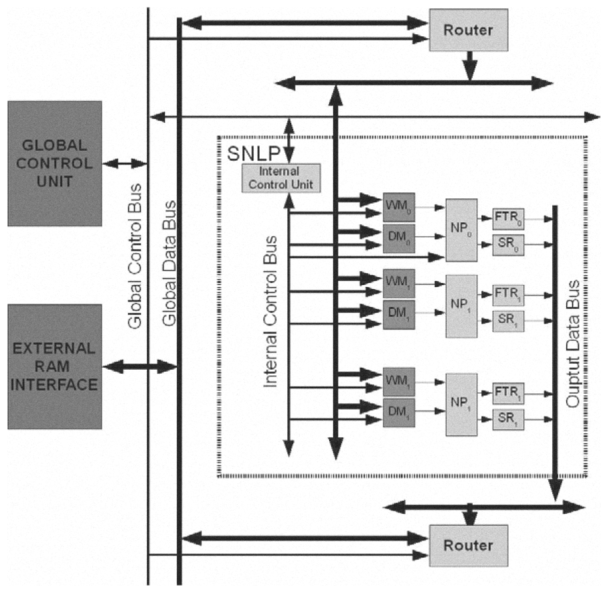
\includegraphics[width=0.9\textwidth]{Figs/2009_BackPropagationFF02}
\end{columns}
}


\frame
{
\frametitle{\citetitle{\EntradaBibtex} (3)}
\begin{columns}
    \column {0.5\textwidth}
   \begin{itemize}
   \item Un módulo de aprendizaje (LM) se encarga de hacer el ajuste de los pesos dependiendo de la tarea específica que debe ser aprendida.
   \item Un enrutador se encarga de sincronizar la transmisión de los datos entre los módulos dependiendo de la etapa de procesamiento.
   \item Existe un pipeline de $N$ etapas dependiendo del número de SNLPs que se incorporen al sistema.
    \end{itemize} 
    \column {0.5\textwidth} 
    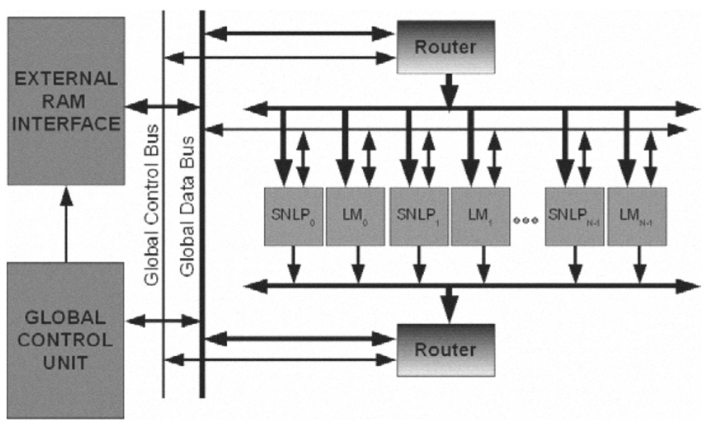
\includegraphics[width=0.9\textwidth]{Figs/2009_BackPropagationFF01}
\end{columns}
}




\frame
{
\frametitle{\citetitle{\EntradaBibtex} (4)}
\begin{columns}
    \column {0.65\textwidth}

\begin{itemize}
\item Se probó con un conjunto de datos de 128 filas por 4 columnas generado aleatoriamente. 
\item Se obtuvó el tiempo de ejecución para diferentes topologías utilizando 2 SNLP con varios NPs (4, 8 y 16). 
\item Las topologías probadas contienen 3 capas de neuronas, y el número de neuronas por capa varía desde 64 neuronas por capa oculta y de salida hasta 256 neuronas por capa oculta y de salida.
\item Se compara el tiempo de ejecución en SW vs el tiempo de ejecución en Hardware para diferentes configuraciones. 
\end{itemize} 

    \column {0.35\textwidth} 
        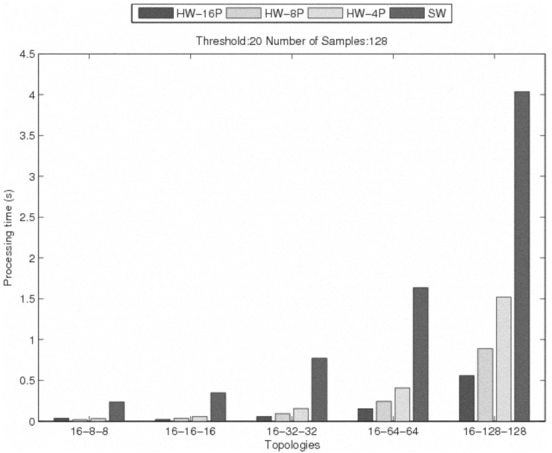
\includegraphics[width=0.9\textwidth]{Figs/2009_BackPropagationFF03}\\
        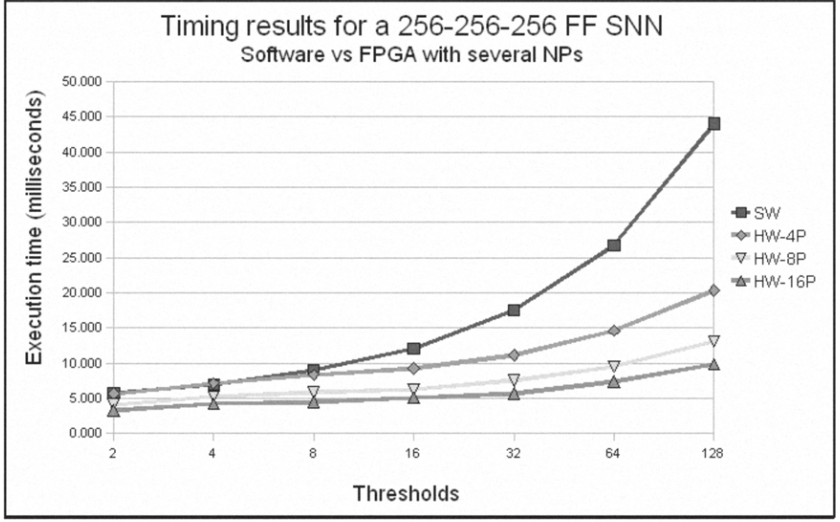
\includegraphics[width=0.9\textwidth]{Figs/2009_BackPropagationFF04}
\end{columns}
}


%
\renewcommand{\EntradaBibtex}{MarcoNuno_CongArbIng_2005_09_00}
%\begin{frame}{\citetitle{\EntradaBibtex} \footnotemark[1] (

\frame
{
\frametitle{\citetitle{\EntradaBibtex} \footnotemark[1] (1)}
\begin{columns}
    \column {0.5\textwidth}
\begin{itemize}    
\item Existe una variedad de técnicas de interpolación que pueden
ser utilizado para funciones tales como ampliar o reducir la
tamaño de una imagen. 
\item Los tres algoritmos muy utilizados son: vecino más cercano,
bilineal y bicúbica.
\end{itemize}
    \column {0.5\textwidth} 
    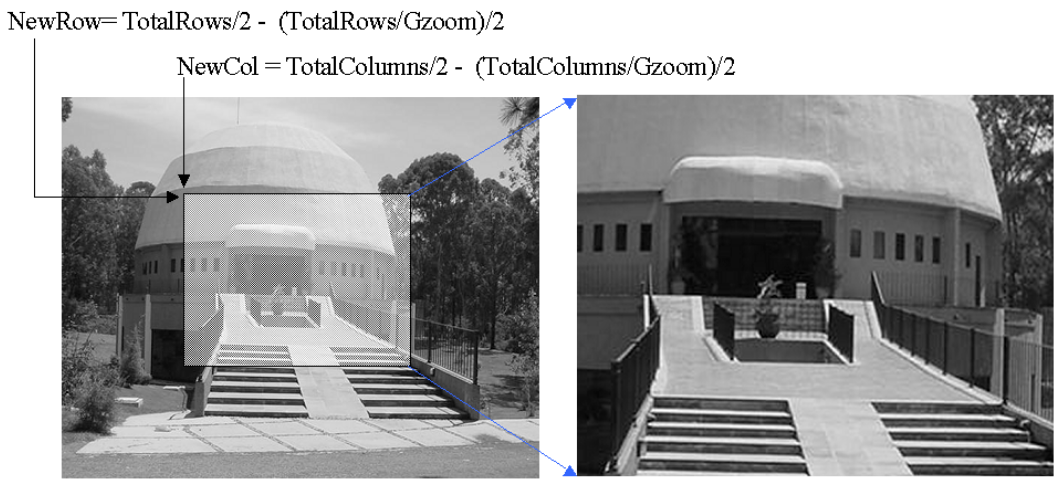
\includegraphics[width=0.9\textwidth]{Figs/BicubicInterpolation02}
\end{columns}     

\footnotetext[1]{\fullcite{\EntradaBibtex}}
}

\frame{
\frametitle{\citetitle{\EntradaBibtex} (2)}
\begin{columns}
    \column {0.5\textwidth}
    \begin{itemize}    
\item Un conjunto de procesadores de zoom (ZP) realizan el
operaciones entre los píxeles de la imagen de entrada y los coeficientes de interpolación, generando como salida el pixel de la  imagen resultante.
\item La interpolación bicúbica requiere una vecindad de 16
píxeles, 16 operaciones de punto flotante y hay similitud
con procesado de ventana.
\item En la implementación actual, se utiliza un Pipeline de $N$ etapas para acelerar el procesamiento de la interpolación.
\end{itemize}

    
    \column {0.5\textwidth} 
    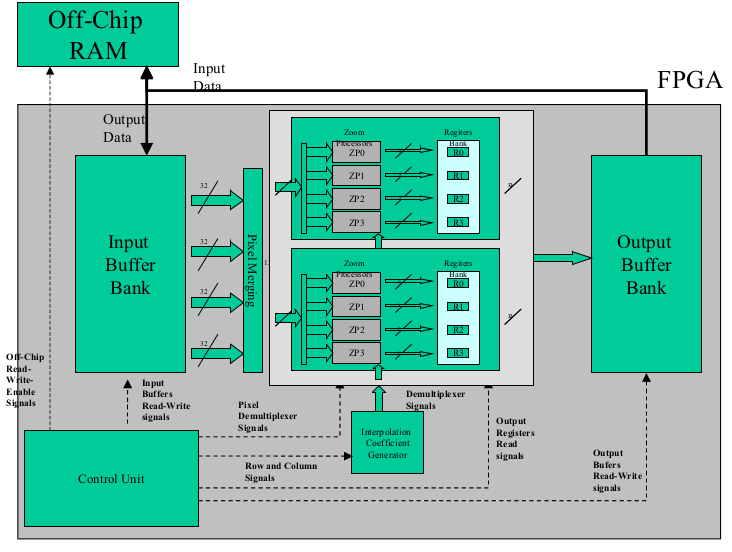
\includegraphics[width=0.9\textwidth]{Figs/BicubicInterpolation01}
\end{columns}     
}

\frame{
\frametitle{\citetitle{\EntradaBibtex} (3)}
\begin{columns}
    \column {0.5\textwidth}
    \begin{itemize} 
\item Se comparó el trabajo propuesto con otros trabajos existentes en la literatura
\item El trabajo propuesto procesa una imágen en 3.5 ms, mientras que el más cercano requería de 11 ms.
\item La implementación de la interpolación del lado de la PC requirió de 50ms para completarse.
\end{itemize}
    \column {0.5\textwidth} 
    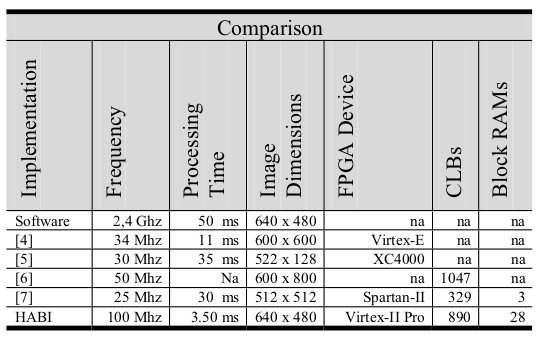
\includegraphics[width=0.9\textwidth]{Figs/BicubicInterpolation03}
\end{columns}     
}

%\renewcommand{\EntradaBibtex}{MarcoNuno_CongArbIng_2003_12_00}
%\begin{frame}{\citetitle{\EntradaBibtex} \footnotemark[1] (


\frame
{
\frametitle{\citetitle{\EntradaBibtex} \footnotemark[1] (1)}
\begin{columns}
  \column {0.5\textwidth}  
En ese artículo se reportan dos arquitecturas hardware:
\begin{itemize}
\item Estimación de la pirámide de imágenes
\item Calcular la correlación entre dos imágenes
\end{itemize}
Tres aplicaciones:
\begin{itemize}
\item Seguimiento.
\item Estabilización.
\item Generación de mosaicos.
\end{itemize}
  \column {0.5\textwidth}  
  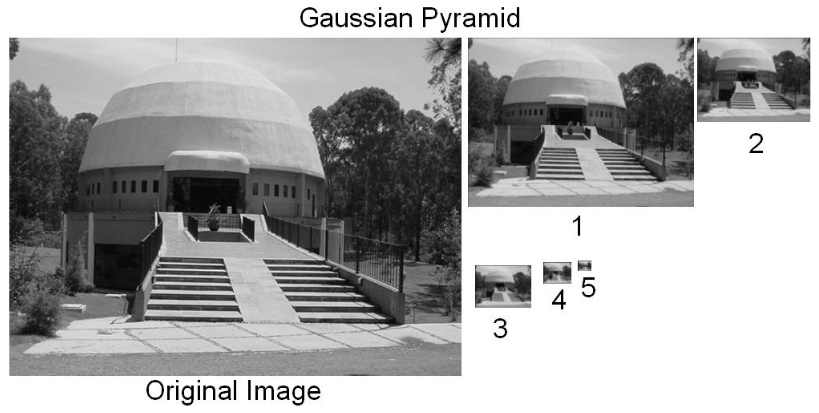
\includegraphics[width=0.9\textwidth]{Figs/Piramide}
  \end{columns}
\footnotetext[1]{\fullcite{\EntradaBibtex}}
}

\frame{
\frametitle{\citetitle{\EntradaBibtex} (2)}
\begin{columns}
    \column {0.5\textwidth}
    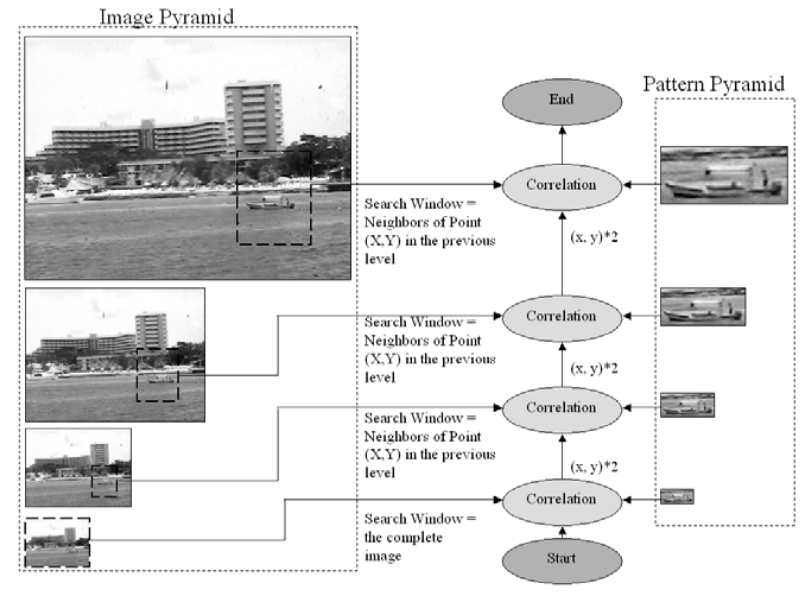
\includegraphics[width=0.9\textwidth]{Figs/Piramide_Correlacion}
    \column {0.5\textwidth}    
        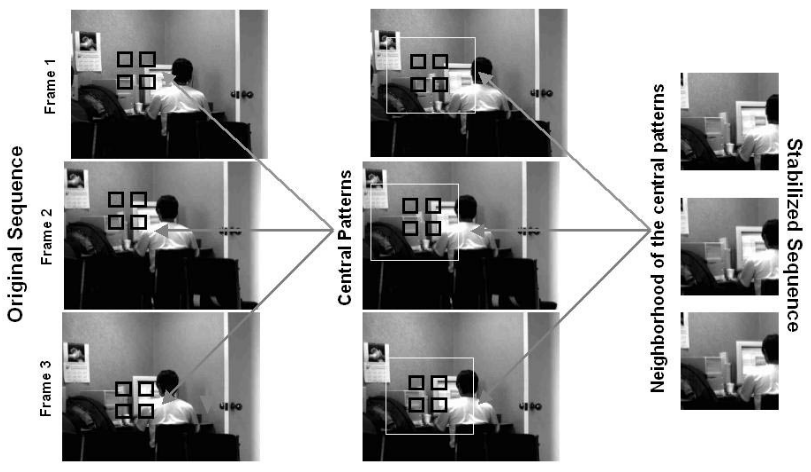
\includegraphics[width=0.8\textwidth]{Figs/Piramide_Estabilizacion}\\
        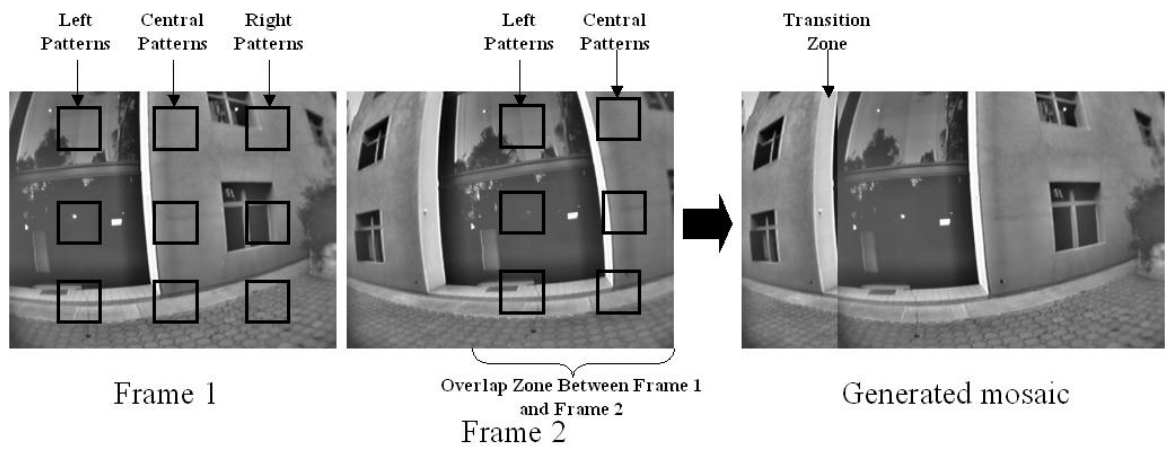
\includegraphics[width=0.98\textwidth]{Figs/Piramide_Mosaicos}
      
\end{columns}    
}

\frame{
\frametitle{\citetitle{\EntradaBibtex} (3)}
    \begin{columns}
        \column {0.5\textwidth}
            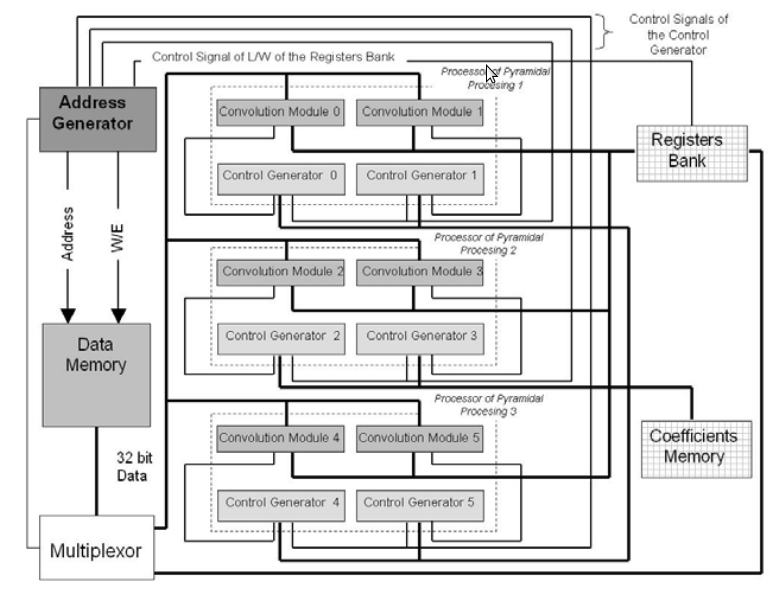
\includegraphics[width=0.8\textwidth]{Figs/Piramide_Arquitectura1}
        \column {0.5\textwidth}    
            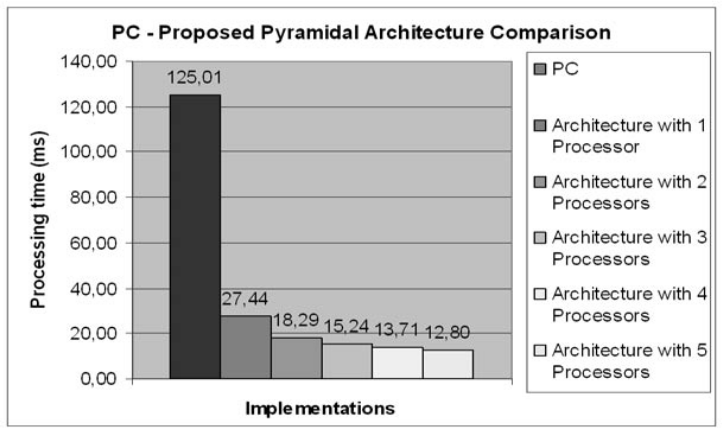
\includegraphics[width=0.9\textwidth]{Figs/Piramide_GraficaComparacion}
    \end{columns}    
}


%\renewcommand{\EntradaBibtex}{MarcoNunoTesisLicenciatura_2002}
%\begin{frame}{\citetitle{\EntradaBibtex} \footnotemark[1] (

\frame
{
\frametitle{\citetitle{\EntradaBibtex} \footnotemark[1] (1)}
\begin{columns}
    \column {0.4\textwidth}
\begin{itemize}    
\item Proyecto de asignatura de maestría: Implementación de la Pirámide en la tarjeta RC100 de Celoxica. 
\item Entrada: Video en RCA, Salida a monitor VGA.
\end{itemize}
    \column {0.3\textwidth}
\begin{center}
    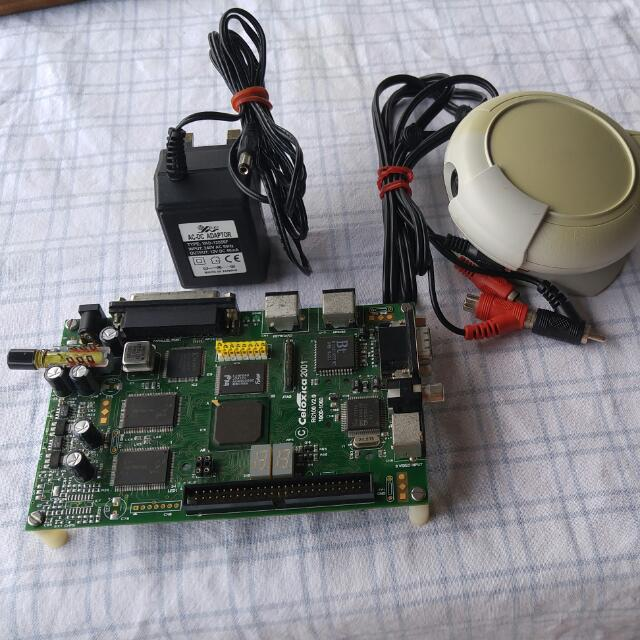
\includegraphics[width=0.9\textwidth]{Figs/celoxica_2001_rc100}
\end{center}    

    \column {0.3\textwidth} 
    \begin{center}
    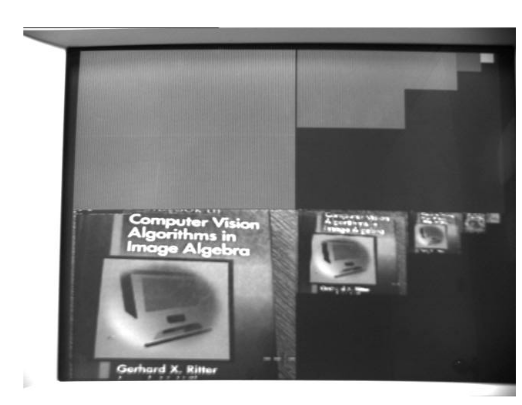
\includegraphics[width=0.9\textwidth]{Figs/2002_PiramideMonitor_RC100}\\
        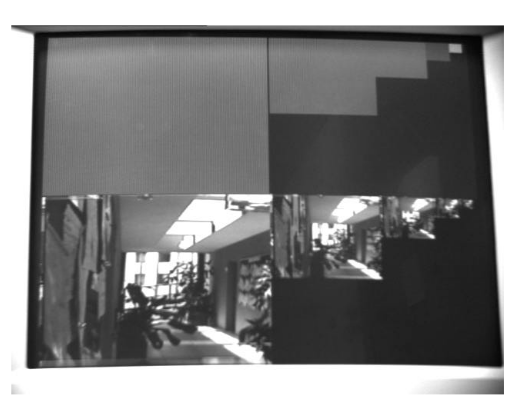
\includegraphics[width=0.9\textwidth]{Figs/2002_PiramideMonitor_RC100_2}
            \end{center}
\end{columns}     

\footnotetext[1]{\fullcite{\EntradaBibtex}}
}

\frame{
\frametitle{Arquitectura Propuesta}
\begin{columns}
    \column {0.5\textwidth}
 \begin{itemize} 
\item Procesamiento de video en tiempo real.
\item Procesamiento simultaneo (doble búffer): Un proceso almacenaba un frame de memoria, mientras que otro procesaba el frame previamente almacenado.
\item Lenguaje: Handel-C (RIP).
\item DK1 Design Suite.
\item FPGA: Spartan-II.
\item Tarjeta: RC-100 de Celoxica.
    
\end{itemize}
    
    \column {0.5\textwidth} 
    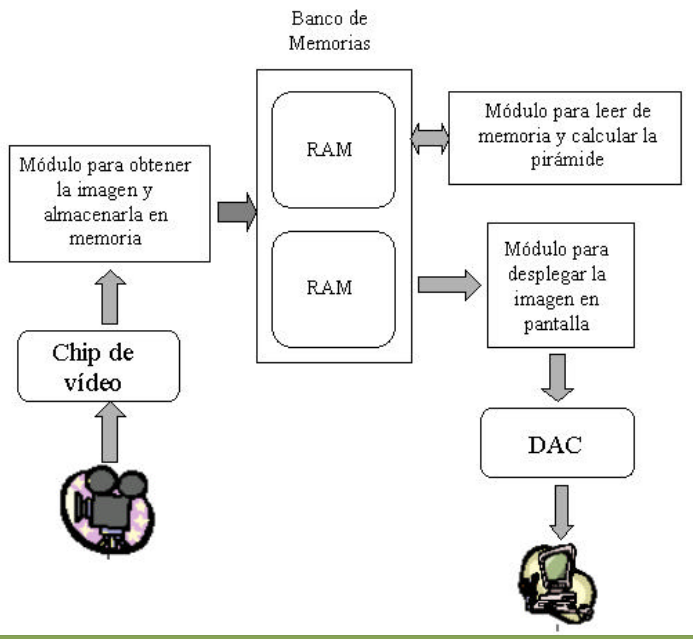
\includegraphics[width=0.9\textwidth]{Figs/2002_PiramideMonitor_RC100_Arquitectura_3}
\end{columns}     
}



%
\renewcommand{\EntradaBibtex}{MarcoNuno_Revista_2025_09_02}

\begin{frame}{\citetitle{\EntradaBibtex}$^*$ (1)}
\begin{block}{Motivación} 
Es necesario automatizar el proceso de evaluación a nivel estatal de estudiantes de nivel medio superior
\end{block} 

\begin{itemize}
\item Se tuvo acceso a un repositorio de 6000 imágenes de digitalizaciones de examenes
\item Detectar los reactivos asignados de manera exacta (con el mínimo de errores) y generar un Excel con dicha información
\item Problemas: Variación en la iluminación, errores en el escaneo, forma de rellenar el circulo por parte de los estudiantes, etc.
\item Estos reactivos alimentan a otro sistema para obtener el resultado de la evaluación
\end{itemize}

\footfullcite*{\EntradaBibtex}
\end{frame}


\begin{frame}{\citetitle{\EntradaBibtex} (2)}
\begin{columns}

% Column 1
\column{.75\linewidth}
\begin{itemize}
\item Detectar rectangulos contenedores. Identificador (Superior) y Respuestas (Inferior)
\item Para los IDs:
\begin{itemize}
\item Se analiza por filas para obtener el ID
\item Opciones para cada fila del ID: 0-9, en blanco (X) o múltiple (M)
\item 4607 para el exámen mostrado
\end{itemize}
\item Para las respuestas:
\begin{itemize}
\item Deliminar una rejilla en donde se infieren están los aciertos.
\item Opciones para el acierto: A/B/C/D, en blanco (X) o múltiple (M)
\end{itemize}
\end{itemize}
\column{.25\linewidth}
	\begin{center}
	%\begin{tabular}{cc}
		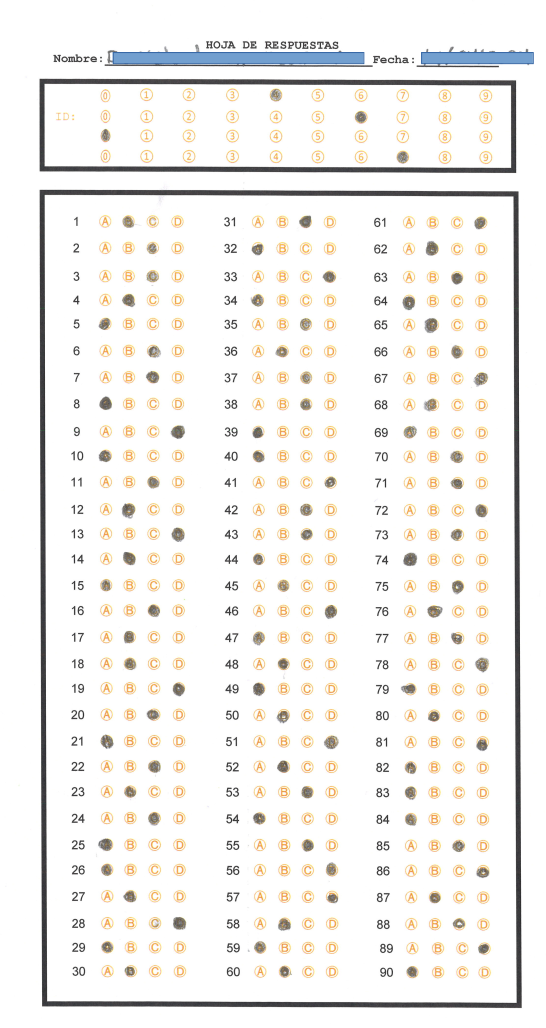
\includegraphics[width=0.90\linewidth]{2025_ProyectoCalificadorExamenes/figs/ExamenES1.png}
		%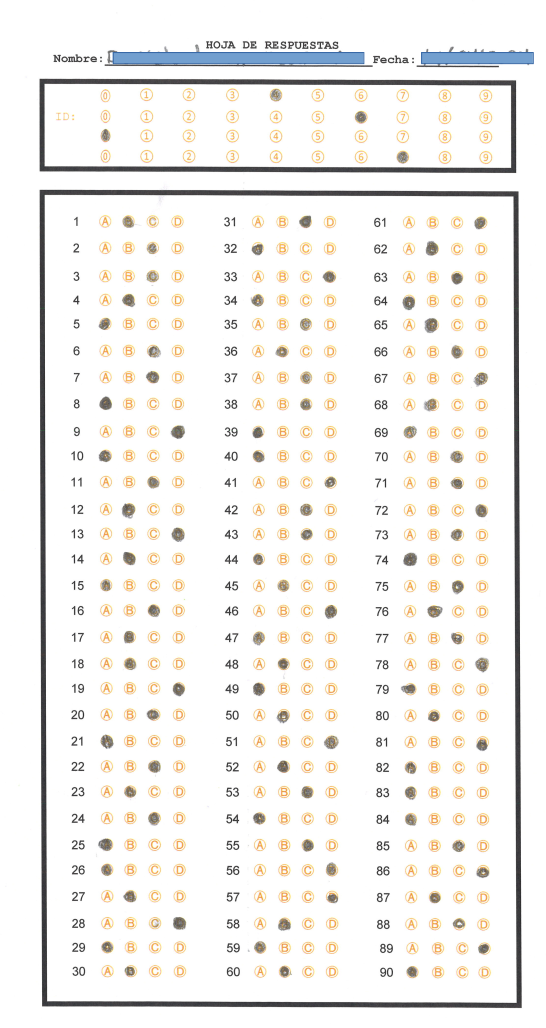
\includegraphics[width=0.20\linewidth]{2025_ProyectoCalificadorExamenes/figs/ExamenES1.png} \\
	%\end{tabular}
\end{center}

\end{columns}

\end{frame}


\begin{frame}{\citetitle{\EntradaBibtex} (3)}
Problemas Detectados
\begin{center}
	\begin{tabular}{ccc}
		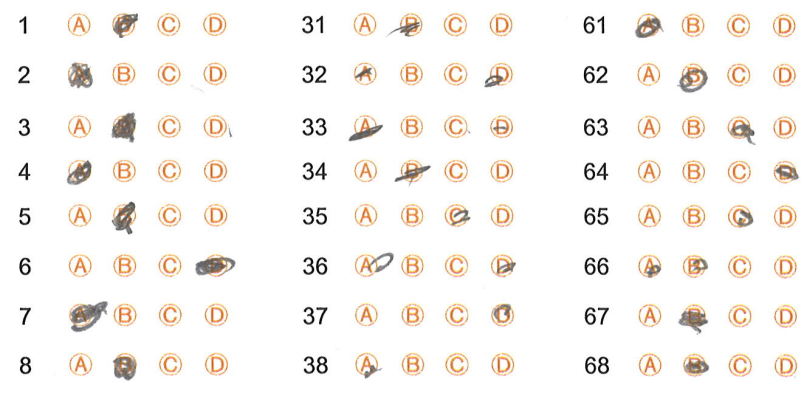
\includegraphics[width=0.35\linewidth]{2025_ProyectoCalificadorExamenes/figs/CasoFlojera.png}&
		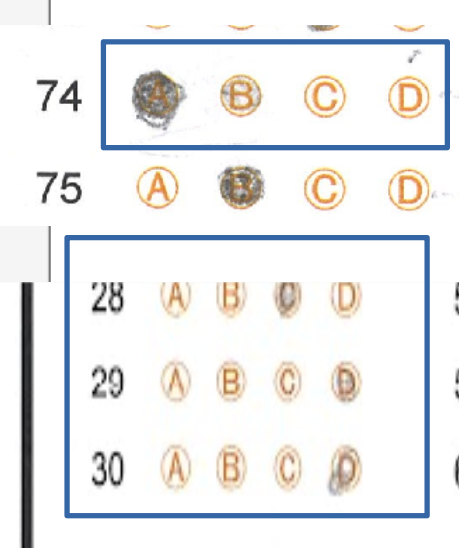
\includegraphics[width=0.10\linewidth]{2025_ProyectoCalificadorExamenes/figs/CasosBorrosos.png} &
		\includegraphics[width=0.15\linewidth]{2025_ProyectoCalificadorExamenes/figs/RespuestaMultiple.png} \\
		Circulos no completos & Borrado de respuesta & Respuesta Multiple \\ 

	\end{tabular}
\end{center}
Estado:
\begin{itemize}
\item Se está evaluando la precisión del sistema (Se estima por arriba del 95\%)
\item Se generó una interfaz para seleccionar carpetas de examenes. Organizados por centro de institucion y semestre (2do, 4to y 6to) y se genera el archivo de Excel con las respuestas
\end{itemize}



\end{frame}


%\renewcommand{\EntradaBibtex}{MarcoNuno_Revista_2025_10_28}

%\begin{frame}{\citetitle{MarcoNuno_ReporteTecnico2022}  \footnotemark{} (1)}
%\begin{frame}{\citetitle{MarcoNuno_ReporteTecnico2022}  \footnote{\fullcite{MarcoNuno_ReporteTecnico2022}} (1)}
\begin{frame}{\citetitle{\EntradaBibtex} \footnotemark[1] (1)}
%\begin{frame}{}
%\footfullcite*{MarcoNuno_ReporteTecnico2022}
\begin{columns}
\begin{column}{0.6\textwidth}
	\begin{itemize}  %del cuerpo académico Acuicultura Sustentable (UTMTB-CA-1)
        \item Proyecto desarrollado  en colaboración con investigadores de la Universidad Tecnológica del Mar de Tamaulipas Bicentenario (UTMarT)
		\item Desarrollar una herramienta para automatizar el conteo de microalgas, específicamente de las especies \textit{Isochrysis galbana} e \textit{Chaetoceros muelleri}
        \item Herramientas Software a utilizar: Python (PC), OpenCV, y Android Studio
        \item Herramientas Hardwware a utilizar: Teléfono inteligente (para captura imágenes), adaptador teléfono-microscopio
	\end{itemize}
\end{column}
\begin{column}{0.4\textwidth}  
\begin{center}
     \begin{tabular}{cc}
         \includegraphics[width=0.68\textwidth]{2025_ConteoMicroAlgas/figs/MicroAlgas01}\\         
      \end{tabular}
\end{center}
\end{column} 
\end{columns} 


%\footnotetext[1]{\fullcite{MarcoNuno_ReporteTecnico2022}}
%\setcounter{footnote}{0}
%\footnotetext{\fullcite{MarcoNuno_ReporteTecnico2022}}
%\footfullcite{MarcoNuno_ReporteTecnico2022}
\footnotetext[1]{\fullcite{\EntradaBibtex}}
\end{frame}


\begin{frame}{\citetitle{\EntradaBibtex} (2)}
\begin{columns}
\begin{column}{0.6\textwidth}
Problemas Encontrados:
\begin{itemize}
        \item Rotación de la rejilla de referencia
        \item Nivel de acercamiento es variable
		\item Imágenes con ruido, distancia de captura variable, regionres con desenfoque 
        \item Problemas de contraste (complica encontrar las lineas)
        \item Cuando hay muchas algas, hay grupos de algas que suelen formar lineas falsas
	\end{itemize}
\end{column}
\begin{column}{0.4\textwidth}  
\begin{center}
     \begin{tabular}{cc}
         \includegraphics[width=0.38\textwidth]{2025_ConteoMicroAlgas/figs/CuadranteA}&
         \includegraphics[width=0.38\textwidth]{2025_ConteoMicroAlgas/figs/CuadranteB}\\
         \includegraphics[width=0.38\textwidth]{2025_ConteoMicroAlgas/figs/CuadranteC}&
         \includegraphics[width=0.38\textwidth]{2025_ConteoMicroAlgas/figs/CuadranteD}\\
          \end{tabular}
\end{center}
\end{column} 
\end{columns} 
\end{frame}


\begin{frame}{\citetitle{\EntradaBibtex} (3)}
\begin{columns}
\begin{column}{0.50\textwidth}
Fases del algoritmo en desarrollo:
\begin{itemize}
		\item Binalizar las imágenes y aplicar un algoritmo de detección de bordes
        \item Encontrar las líneas mediante los algoritmos de Hough Standard y Probabilístico
        \item Analizar las líneas encontradas para determinar aquellas que deben descartarse 
        \item Efectuar un enmascarado de regiones para aislar solo la rejilla delimitadora
        \item Llevar a cabo el conteo de las algas a partir de los contornos de la imágen de bordes
	\end{itemize}
\end{column}
\begin{column}{0.50\textwidth}  
\begin{center}
     \begin{tabular}{ccc}
         \includegraphics[width=0.31\textwidth]{2025_ConteoMicroAlgas/figs/MicroAlgas01}&
         \includegraphics[width=0.31\textwidth]{2025_ConteoMicroAlgas/figs/02_Canny}&
         \includegraphics[width=0.31\textwidth]{2025_ConteoMicroAlgas/figs/03_LineasEstandar}\\
         \includegraphics[width=0.31\textwidth]{2025_ConteoMicroAlgas/figs/04_LineasProbabilistico}&
         \includegraphics[width=0.31\textwidth]{2025_ConteoMicroAlgas/figs/05_Delimitacion}&
         \includegraphics[width=0.31\textwidth]{2025_ConteoMicroAlgas/figs/07_ResultadoConteo}\\

          \end{tabular}
\end{center}
\end{column} 
\end{columns} 
\end{frame}



\begin{frame}{\citetitle{\EntradaBibtex} (4)}

\begin{itemize}
\item Hay un avance significativo con respecto al prototipo versión PC (cerca de completarse)
\begin{itemize} 
\item Se requieren más imágenes, que incluyan el conteo realizado de manera manual para contrastarlo con nuestros algoritmos
\item Posiblemente se deban afinar los algoritmos que se tienen desarrollados
\end{itemize}
\item Con respecto a la fase en el teléfono inteligente, se lleva un avance del 20\%, a reserva de la incorporación de un estudiante de estancia o estadía
\item Los resultados apuntan que es posible publicar los resultados en una Revista Indexada por el JCR
\end{itemize}
\end{frame}





\renewcommand{\EntradaBibtex}{MarcoNuno_Revista_2026_02_01}

\begin{frame}{\citetitle{\EntradaBibtex}$^*$ (1)}
\begin{block}{Problema y objetivo} 
Desarrollar una plataforma robótica educativa accesible para desarrollar y evaluar el Pensamiento Computacional.
\end{block} 

La educación STEM/STEAM busca desarrollar competencias como:
\begin{itemize}
\item Programación y resolución de problemas.
\item Pensamiento computacional (CT) y trabajo colaborativo.
\end{itemize}
Sin embargo, muchas plataformas de robótica y simulación:
\begin{itemize}
  \item Tienen un costo elevado.
  \item  Requieren computadoras con mayores recursos.
  \item  Funcionan únicamente de manera virtual o física.
\end{itemize}


\footfullcite*{\EntradaBibtex}
\end{frame}


\begin{frame}{\citetitle{\EntradaBibtex} (2)}
\begin{block}{Arquitectura: Integración hardware + software + simulación} 
\begin{center}
\includegraphics[width=0.6\linewidth]{2026_Mobile2D-3D-RoboticSim/figs/1-s2.0-S235271102500439X-gr1_lrg.jpg}
\end{center}

\end{block} 
\end{frame}


\begin{frame}{\citetitle{\EntradaBibtex} (3)}
\begin{columns}
\begin{column}{0.40\textwidth}
Simulador 2D

\begin{itemize}
		\item  Entorno basado en una cuadrícula 10 × 10.
		\item  El usuario define comandos de movimiento.
		\item  Permite colocar obstáculos.
		\item  Simula la evasión de obstáculos.
		\item  Puede funcionar con o sin robot físico.
	\end{itemize}
\end{column}
\begin{column}{0.60\textwidth}  
\begin{center}
\includegraphics[width=0.98\textwidth]{2026_Mobile2D-3D-RoboticSim/figs/1-s2.0-S235271102500439X-gr4_lrg.jpg}
\end{center}
\end{column} 
\end{columns} 
\end{frame}


\begin{frame}{\citetitle{\EntradaBibtex} (4)}
\begin{columns}
\begin{column}{0.40\textwidth}
Simulador 3D
\begin{itemize}
\item Modelo tridimensional del robot.
\item Visualización de trayectorias.
\item Modos manual y automático.
\item Conversión de rutas 2D a trayectorias 3D.
\item Sincronización con el robot físico.
	\end{itemize}
\end{column}
\begin{column}{0.60\textwidth}  
\begin{center}
\includegraphics[width=0.98\textwidth]{2026_Mobile2D-3D-RoboticSim/figs/1-s2.0-S235271102500439X-gr5_lrg.jpg}
\end{center}
\end{column} 
\end{columns} 
\end{frame}

\begin{frame}{\citetitle{\EntradaBibtex} (5)}
\begin{block}{Conclusiones} 
Una plataforma híbrida para STEM/STEAM cuyas principales aportaciones son:
\begin{itemize}
\item Plataforma robótica de bajo costo.
\item Integración de robot físico + simulación 2D + simulación 3D.
\item Uso desde dispositivos móviles.
\item Posibilidad de trabajar incluso cuando el robot físico no está disponible.
\item Sincronización entre el mundo virtual y el físico.
\item Aplicación potencial para desarrollar y evaluar pensamiento computacional.
\end{itemize}
Trabajo futuro:
\begin{itemize}
\item Incorporar sensores adicionales.
\item Mejorar la percepción del entorno.
\item Transmitir video en tiempo real desde el robot.
\end{itemize}
\end{block}
\end{frame}

\renewcommand{\EntradaBibtex}{2026_RecorridoUPV_mas_Jaguar}

\begin{frame}{\citetitle{\EntradaBibtex}$^*$ (1)}
\begin{block}{Problema y objetivo} 
El proyecto evoluciona un simulador de recorridos virtuales del campus de la Universidad Politécnica de Victoria para iOS (anteriormente solo para dispositivos Android).
\end{block} 

Esta tercera iteración busca resolver dos limitaciones:
\begin{itemize}
\item El campus era un espacio sin personajes o vida simulada.
\item El recorrido solamente podía experimentarse en primera persona.Programación y resolución de problemas.
\end{itemize}
Se incorporan:
\begin{itemize}
  \item NPC (Non-Player Character) jaguar autónomo que recorre el campus.
  \item Cámara en tercera persona para visualizar al jugador.
\end{itemize}
\footfullcite*{\EntradaBibtex}
\end{frame}

\begin{frame}{\citetitle{\EntradaBibtex} (2)}
\begin{block}{Arquitectura y componentes} 

Componentes de la arquitectura:
\begin{itemize}
\item UPVScene: controlador principal de la escena.
\item ConstructorEdificio: geometría y sistema de colisiones.
\item Campus y Ambiente: elementos del mundo exterior.
\item Módulos adicionales:
\begin{itemize}
\item Jaguar. Modelo 3D, pelaje procedural y avatar animado
\item JaguarNPC.	Navegación autónoma
\item UPVScene.	Cámara en tercera persona y coordinación
\item ContentView.	Controles y posición del NPC en minimapa
\end{itemize}
\end{itemize}

\end{block} 

\end{frame}



%\renewcommand{\EntradaBibtex}{pr14010164}

\begin{frame}{\citetitle{\EntradaBibtex} \footnotemark[1] (1)}
Problemática: 
\begin{itemize}
    \item Las máquinas industriales de clasificación de fruta utilizan tecnología que lleva muchos años en funcionamiento.
    \item Los algoritmos de clasificación son cerrados y no es posible agregar adecuaciones. 

\end{itemize}
\footnotetext[1]{\fullcite{\EntradaBibtex}}
\end{frame}

\begin{frame}{\citetitle{\EntradaBibtex} (2)}
Propuesta de solución: 
\begin{itemize}
    \item Se desarrolló  un sistema de visión por computadora para clasificar limones por tamaño en tiempo real, integrado directamente en una máquina clasificadora de nivel industrial.
    \item Se evaluaron modelos de aprendizaje automático combinados con análisis de imágenes para estimar las dimensiones (diámetro/tamaño) de los cítricos de forma automática.
    \item Se incorporó un algoritmo de gestión de colas para coordinar el procesamiento de imágenes con el desplazamiento físico de las frutas en la cinta transportadora, garantizando la sincronización precisa entre la detección y los desviadores mecánicos (ejectors).
\end{itemize}

\end{frame}

\begin{frame}{\citetitle{\EntradaBibtex} (3)}
\begin{columns}
\begin{column}{0.45\textwidth}
Materiales:
\begin{itemize}
    \item Una computadora embebida (SBC - Raspberry Pi 4 model B+) 
    \item Una cámara industrial USB 3.0 (HT-SUA134GC-T1V Huateng)
    \item Un microcontrolador Arduino Mega 2560.
    \item Anillo de iluminación led.
    \item Driver para solenoides.                 
\end{itemize}
\end{column}
\begin{column}{0.25\textwidth}
\begin{center}
\includegraphics[width=0.90\linewidth]{2026_Citricos/figs/BandaTransportadoraA.png}    
\end{center}   
\end{column}
\begin{column}{0.25\textwidth}
\begin{center}
\includegraphics[width=0.90\linewidth]{2026_Citricos/figs/Prototype.jpg}    
\end{center}   
\end{column}

\end{columns}
\end{frame}


\begin{frame}{\citetitle{\EntradaBibtex} (4)}
\begin{center}
\includegraphics[width=0.50\linewidth]{2026_Citricos/figs/SortingMachine.png}    
\end{center}    
\end{frame}



\begin{frame}{\citetitle{\EntradaBibtex} (5)}
\begin{center}
\includegraphics[width=0.92\linewidth]{2026_Citricos/figs/ImageProcessingPipeline_processes-14-00164-g006.png}    
\end{center}    
\end{frame}

\begin{frame}{\citetitle{\EntradaBibtex} (6)}
\begin{columns}
\begin{column}{0.75\textwidth}
Medición del tamaño de los limones: \\
\begin{itemize}
    \item Se utiliza un calibrador mecánico para medir el tamaño de los limones según los estándares de la industria citrícola. 
    \item El dispositivo cuenta con mordazas ajustables que miden el diámetro del eje menor del limón, y que determina el código de tamaño de la fruta (``cantidad''), que indica cuántos limones caben en una caja estándar de 40 libras. Estos tamaños son (75, 95, 115, 140, 165, y 200). 
\end{itemize}
Problema: \\
\begin{itemize}
    \item Los rangos de medición disponibles se superponen, lo que puede generar errores de clasificación, y que esto suele estar sujeto a la interpretación del usuario.
\end{itemize}

\end{column}
\begin{column}{0.25\textwidth}
\begin{center}
\includegraphics[width=0.95\textwidth]{2026_Citricos/figs/califer.jpg}  
\tiny{\url{https://qasupplies.com/citrus-produce-calipers/}}
\end{center}    
\end{column}
\end{columns}
\end{frame}



\begin{frame}{\citetitle{\EntradaBibtex} (7)}
\begin{columns}
\begin{column}{0.45\textwidth}
Validación del modelo en campo: \\
\begin{itemize}
    \item Se utilizó una muestra de limones independiente al dataset utilizado para entrenar el modelo
    \item Se clasificaron 1,558 limones distribuidos en las siguients clases: 175 (95), 241 (115), 308 (140), 390 (165) y 444 (200). 
    \item Se alcanzó una exactitud del 78\%.
\end{itemize}

\end{column}
\begin{column}{0.45\textwidth}
\begin{center}
\includegraphics[width=0.90\linewidth]{2026_Citricos/figs/ConfusionMatrix_processes-14-00164-g013.png}    
\end{center}   
\end{column}

\end{columns}
 
\end{frame}


%\renewcommand{\EntradaBibtex}{virtualworlds5040053}

\begin{frame}{\citetitle{\EntradaBibtex} \footnotemark[1] (1)}
Visualización de materiales híbridos multifuncionales
\begin{itemize}
\item Los materiales híbridos pueden integrar múltiples fases activas dentro de una misma estructura.
\item Su comportamiento depende de la interacción entre diferentes componentes.
\item Los diagramas 2D tradicionales dificultan comprender:
\begin{itemize}
  \item La distribución espacial de los componentes.
  \item La relación entre estructura y función.
  \item Los mecanismos de interacción.
\end{itemize}
\item Se propone utilizar visualización 3D interactiva y realidad aumentada (RA) para mejorar la comunicación científica, la cual permite explorar la estructura de un material complejo de una manera más intuitiva.
\end{itemize}
%La visualización inmersiva permite explorar la estructura de un material complejo de una manera más intuitiva que una representación estática.
\footnotetext[1]{\fullcite{\EntradaBibtex}}
\end{frame}

\begin{frame}{\citetitle{\EntradaBibtex} (2)}

Multifunctional Hybrid Material (MHM-App)

La aplicación representa una esfera multifuncional formada por:
\begin{itemize}
\item TiO$_2$: fase fotocatalítica.
\item Fe$_3$O$_4$ (magnetita): fase magnética.
\item Carbón activado: material adsorbente.
\item Clinoptilolita con hipoclorito: agente de liberación/control.
\item CuO: componente con función antimicrobiana.
\item Alginato de sodio: matriz encapsulante formada mediante gelación iónica.
\item Quitosano reticulado: recubrimiento externo.
\end{itemize}
La aplicación permite observar simultáneamente la estructura global y los diferentes materiales que la constituyen.
\end{frame}



\begin{frame}{\citetitle{\EntradaBibtex} (3)}

Aplicación móvil de visualización 3D + RA, proporciona dos modos complementarios:

\begin{columns}

% Column 1
\column{.4\linewidth}

\item Modo Realidad Aumentada
\begin{itemize}
\item Detecta una superficie horizontal.
\item Utiliza raycasting para colocar la esfera.
\item Permite observar el material integrado en el entorno real.
\end{itemize}

\column{.6\linewidth}
\begin{center}
\includegraphics[width=0.20\linewidth]{2026_Augmented_Reality_Multifunctional_Hybrid_Materials/figs/hscm1_en.PNG}
\includegraphics[width=0.20\linewidth]{2026_Augmented_Reality_Multifunctional_Hybrid_Materials/figs/hscm2_en.PNG}
\includegraphics[width=0.20\linewidth]{2026_Augmented_Reality_Multifunctional_Hybrid_Materials/figs/hscm4_en.PNG}
\includegraphics[width=0.20\linewidth]{2026_Augmented_Reality_Multifunctional_Hybrid_Materials/figs/hscm7_en.PNG}                                
\end{center}   
\end{columns}
\end{frame}


\begin{frame}{\citetitle{\EntradaBibtex} (4)}
\begin{columns}
% Column 1
\column{.4\linewidth}
Modo no-RA / entorno virtual
\begin{itemize}
\item La misma geometría 3D se presenta en una escena virtual.
\item Cámara con perspectiva fija.
\item Iluminación explícita para facilitar la inspección.
\end{itemize}
\column{.6\linewidth}
\begin{center}
\includegraphics[width=0.20\linewidth]{2026_Augmented_Reality_Multifunctional_Hybrid_Materials/figs/hscm11_en.PNG}
\includegraphics[width=0.20\linewidth]{2026_Augmented_Reality_Multifunctional_Hybrid_Materials/figs/hscm12_en.PNG}
\includegraphics[width=0.20\linewidth]{2026_Augmented_Reality_Multifunctional_Hybrid_Materials/figs/hscm13_en.PNG}
\includegraphics[width=0.20\linewidth]{2026_Augmented_Reality_Multifunctional_Hybrid_Materials/figs/hscm14_en_new.PNG}                                
\end{center}   
\end{columns}
\end{frame}


\begin{frame}{\citetitle{\EntradaBibtex} (5)}
Contribución principal
\begin{itemize}
\item Integración de RA + visualización 3D interactiva en una aplicación móvil.
\item Representación de la coexistencia espacial de múltiples fases dentro de un material híbrido.
\end{itemize}

Aplicaciones potenciales
\begin{itemize}
\item Educación: enseñanza de materiales y procesos químicos.
\item Comunicación científica: explicación de estructuras complejas.
\item Colaboración interdisciplinaria: interacción entre especialistas.
\item Ciencia de materiales: exploración de estructuras multifuncionales.
\end{itemize}
MHM-App demuestra el potencial de la RA y la visualización 3D móvil como herramientas para comprender, comunicar y explorar materiales multifuncionales complejos.
\end{frame}



\end{document}

